\documentclass[lettersize,onecolumn,journal]{IEEEtran}
%DIF LATEXDIFF DIFFERENCE FILE
%DIF DEL ieee_v1.tex   Sun Jan 16 22:34:55 2022
%DIF ADD ieee_v2.tex   Sun Jan 16 22:34:55 2022
\usepackage{amsmath,amsfonts}
%DIF 3d3
%DIF < %\usepackage{algorithmic}
%DIF -------
\usepackage{algorithm}
\usepackage{array}
\usepackage[caption=false,font=normalsize,labelfont=sf,textfont=sf]{subfig}
\usepackage{textcomp}
\usepackage{stfloats}
\usepackage{url}
\usepackage{verbatim}
\usepackage{graphicx}
\usepackage{cite}
\hyphenation{op-tical net-works semi-conduc-tor IEEE-Xplore}
% updated with editorial comments 8/9/2021

\usepackage{algpseudocode}
\usepackage{amsmath}
\usepackage{graphicx}
\usepackage{enumerate}
\usepackage[authoryear]{natbib}
\usepackage{url}
\usepackage{enumitem}


\usepackage{amsmath,amssymb,amsthm,bm,mathtools}
\usepackage{algorithm}
\usepackage{dsfont,multirow,hyperref,setspace,enumerate}
\hypersetup{colorlinks,linkcolor=black,citecolor=black,urlcolor={black}}
\usepackage{lscape}
\usepackage{afterpage}
\usepackage{hyperref}

\usepackage{microtype}
\usepackage{wrapfig}
\allowdisplaybreaks
\usepackage{algorithm}
\usepackage{algpseudocode}

\usepackage{tabularx,booktabs}
\newcolumntype{Y}{>{\centering\arraybackslash}X}




\theoremstyle{definition}
\newtheorem{thm}{Theorem}
\newtheorem{lem}{Lemma}
\newtheorem{prop}{Proposition}[section]
\newtheorem{pro}{Property}
\newtheorem{cor}{Corollary}

\theoremstyle{definition}
\newtheorem{assumption}{Assumption}
\newtheorem{defn}{Definition}
\newtheorem{example}{Example}
\newtheorem{rmk}{Remark}
\newtheorem{condition}{Condition}
\newtheorem{conjecture}{Conjecture}
\newtheorem{property}{Property}
\newtheorem{hypothesis}{Hypothesis}

\newtheorem{innercustomgeneric}{\customgenericname}
\providecommand{\customgenericname}{}
\newcommand{\newcustomtheorem}[2]{%
  \newenvironment{#1}[1]
  {%
   \renewcommand\customgenericname{#2}%
   \renewcommand\theinnercustomgeneric{##1}%
   \innercustomgeneric
  }
  {\endinnercustomgeneric}
}


\newcustomtheorem{customexample}{Example}

%DIF 77d76
%DIF < %\usepackage{appendix}
%DIF -------
\usepackage{fullpage} 
\usepackage{microtype}
\usepackage{wrapfig}
\mathtoolsset{showonlyrefs}

\newcommand{\of}[1]{\left(#1\right)}
\newcommand{\off}[1]{\left[#1\right]}
\newcommand{\offf}[1]{\left\{#1\right\}}
\newcommand{\aabs}[1]{\left|#1\right|}
\newcommand{\ang}[1]{\left\langle#1\right\rangle}


%DIF 90d88
%DIF < \newcommand{\distgap}{D_{\ell_2}}
%DIF -------
\newcommand{\Mat}{\text{Mat}}


\def\ci{\perp\!\!\!\perp}


\usepackage{booktabs}
\newcommand\doubleRule{\toprule\toprule}
\allowdisplaybreaks

\newcommand*{\KeepStyleUnderBrace}[1]{%f
  \mathop{%
    \mathchoice
    {\underbrace{\displaystyle#1}}%
    {\underbrace{\textstyle#1}}%
    {\underbrace{\scriptstyle#1}}%
    {\underbrace{\scriptscriptstyle#1}}%
  }\limits
}



\input macros.tex
\newcommand*{\Scale}[2][4]{\scalebox{#1}{$#2$}}%
\setlength\parindent{0pt}
\usepackage[parfill]{parskip}
\usepackage{algorithm}
\usepackage{algpseudocode}
\usepackage{amsmath}


\DeclarePairedDelimiter{\ceil}{\lceil}{\rceil}
\DeclarePairedDelimiter{\floor}{\lfloor}{\rfloor}

\algnewcommand\algorithmicinput{\textbf{Input:}}
\algnewcommand\algorithmicoutput{\textbf{Output:}}
\algnewcommand\INPUT{\item[\algorithmicinput]}
\algnewcommand\OUTPUT{\item[\algorithmicoutput]}

\newcommand\Algphase[1]{%
\vspace*{-.7\baselineskip}\Statex\hspace*{\dimexpr-\algorithmicindent-2pt\relax}\rule{\columnwidth}{0.4pt}%
\Statex\hspace*{-\algorithmicindent}\textbf{#1}%
\vspace*{-.7\baselineskip}\Statex\hspace*{\dimexpr-\algorithmicindent-2pt\relax}\rule{\columnwidth}{0.4pt}%
}
\usepackage{caption}
\def\fixme#1#2{\textbf{\color{red}[FIXME (#1): #2]}}
%DIF PREAMBLE EXTENSION ADDED BY LATEXDIFF
%DIF UNDERLINE PREAMBLE %DIF PREAMBLE
\RequirePackage[normalem]{ulem} %DIF PREAMBLE
\RequirePackage{color}\definecolor{RED}{rgb}{1,0,0}\definecolor{BLUE}{rgb}{0,0,1} %DIF PREAMBLE
\providecommand{\DIFaddtex}[1]{{\protect\color{blue}\uwave{#1}}} %DIF PREAMBLE
\providecommand{\DIFdeltex}[1]{{\protect\color{red}\sout{#1}}}                      %DIF PREAMBLE
%DIF SAFE PREAMBLE %DIF PREAMBLE
\providecommand{\DIFaddbegin}{} %DIF PREAMBLE
\providecommand{\DIFaddend}{} %DIF PREAMBLE
\providecommand{\DIFdelbegin}{} %DIF PREAMBLE
\providecommand{\DIFdelend}{} %DIF PREAMBLE
\providecommand{\DIFmodbegin}{} %DIF PREAMBLE
\providecommand{\DIFmodend}{} %DIF PREAMBLE
%DIF FLOATSAFE PREAMBLE %DIF PREAMBLE
\providecommand{\DIFaddFL}[1]{\DIFadd{#1}} %DIF PREAMBLE
\providecommand{\DIFdelFL}[1]{\DIFdel{#1}} %DIF PREAMBLE
\providecommand{\DIFaddbeginFL}{} %DIF PREAMBLE
\providecommand{\DIFaddendFL}{} %DIF PREAMBLE
\providecommand{\DIFdelbeginFL}{} %DIF PREAMBLE
\providecommand{\DIFdelendFL}{} %DIF PREAMBLE
%DIF HYPERREF PREAMBLE %DIF PREAMBLE
\providecommand{\DIFadd}[1]{\texorpdfstring{\DIFaddtex{#1}}{#1}} %DIF PREAMBLE
\providecommand{\DIFdel}[1]{\texorpdfstring{\DIFdeltex{#1}}{}} %DIF PREAMBLE
\newcommand{\DIFscaledelfig}{0.5}
%DIF HIGHLIGHTGRAPHICS PREAMBLE %DIF PREAMBLE
\RequirePackage{settobox} %DIF PREAMBLE
\RequirePackage{letltxmacro} %DIF PREAMBLE
\newsavebox{\DIFdelgraphicsbox} %DIF PREAMBLE
\newlength{\DIFdelgraphicswidth} %DIF PREAMBLE
\newlength{\DIFdelgraphicsheight} %DIF PREAMBLE
% store original definition of \includegraphics %DIF PREAMBLE
\LetLtxMacro{\DIFOincludegraphics}{\includegraphics} %DIF PREAMBLE
\newcommand{\DIFaddincludegraphics}[2][]{{\color{blue}\fbox{\DIFOincludegraphics[#1]{#2}}}} %DIF PREAMBLE
\newcommand{\DIFdelincludegraphics}[2][]{% %DIF PREAMBLE
\sbox{\DIFdelgraphicsbox}{\DIFOincludegraphics[#1]{#2}}% %DIF PREAMBLE
\settoboxwidth{\DIFdelgraphicswidth}{\DIFdelgraphicsbox} %DIF PREAMBLE
\settoboxtotalheight{\DIFdelgraphicsheight}{\DIFdelgraphicsbox} %DIF PREAMBLE
\scalebox{\DIFscaledelfig}{% %DIF PREAMBLE
\parbox[b]{\DIFdelgraphicswidth}{\usebox{\DIFdelgraphicsbox}\\[-\baselineskip] \rule{\DIFdelgraphicswidth}{0em}}\llap{\resizebox{\DIFdelgraphicswidth}{\DIFdelgraphicsheight}{% %DIF PREAMBLE
\setlength{\unitlength}{\DIFdelgraphicswidth}% %DIF PREAMBLE
\begin{picture}(1,1)% %DIF PREAMBLE
\thicklines\linethickness{2pt} %DIF PREAMBLE
{\color[rgb]{1,0,0}\put(0,0){\framebox(1,1){}}}% %DIF PREAMBLE
{\color[rgb]{1,0,0}\put(0,0){\line( 1,1){1}}}% %DIF PREAMBLE
{\color[rgb]{1,0,0}\put(0,1){\line(1,-1){1}}}% %DIF PREAMBLE
\end{picture}% %DIF PREAMBLE
}\hspace*{3pt}}} %DIF PREAMBLE
} %DIF PREAMBLE
\LetLtxMacro{\DIFOaddbegin}{\DIFaddbegin} %DIF PREAMBLE
\LetLtxMacro{\DIFOaddend}{\DIFaddend} %DIF PREAMBLE
\LetLtxMacro{\DIFOdelbegin}{\DIFdelbegin} %DIF PREAMBLE
\LetLtxMacro{\DIFOdelend}{\DIFdelend} %DIF PREAMBLE
\DeclareRobustCommand{\DIFaddbegin}{\DIFOaddbegin \let\includegraphics\DIFaddincludegraphics} %DIF PREAMBLE
\DeclareRobustCommand{\DIFaddend}{\DIFOaddend \let\includegraphics\DIFOincludegraphics} %DIF PREAMBLE
\DeclareRobustCommand{\DIFdelbegin}{\DIFOdelbegin \let\includegraphics\DIFdelincludegraphics} %DIF PREAMBLE
\DeclareRobustCommand{\DIFdelend}{\DIFOaddend \let\includegraphics\DIFOincludegraphics} %DIF PREAMBLE
\LetLtxMacro{\DIFOaddbeginFL}{\DIFaddbeginFL} %DIF PREAMBLE
\LetLtxMacro{\DIFOaddendFL}{\DIFaddendFL} %DIF PREAMBLE
\LetLtxMacro{\DIFOdelbeginFL}{\DIFdelbeginFL} %DIF PREAMBLE
\LetLtxMacro{\DIFOdelendFL}{\DIFdelendFL} %DIF PREAMBLE
\DeclareRobustCommand{\DIFaddbeginFL}{\DIFOaddbeginFL \let\includegraphics\DIFaddincludegraphics} %DIF PREAMBLE
\DeclareRobustCommand{\DIFaddendFL}{\DIFOaddendFL \let\includegraphics\DIFOincludegraphics} %DIF PREAMBLE
\DeclareRobustCommand{\DIFdelbeginFL}{\DIFOdelbeginFL \let\includegraphics\DIFdelincludegraphics} %DIF PREAMBLE
\DeclareRobustCommand{\DIFdelendFL}{\DIFOaddendFL \let\includegraphics\DIFOincludegraphics} %DIF PREAMBLE
%DIF LISTINGS PREAMBLE %DIF PREAMBLE
\RequirePackage{listings} %DIF PREAMBLE
\RequirePackage{color} %DIF PREAMBLE
\lstdefinelanguage{DIFcode}{ %DIF PREAMBLE
%DIF DIFCODE_UNDERLINE %DIF PREAMBLE
  moredelim=[il][\color{red}\sout]{\%DIF\ <\ }, %DIF PREAMBLE
  moredelim=[il][\color{blue}\uwave]{\%DIF\ >\ } %DIF PREAMBLE
} %DIF PREAMBLE
\lstdefinestyle{DIFverbatimstyle}{ %DIF PREAMBLE
	language=DIFcode, %DIF PREAMBLE
	basicstyle=\ttfamily, %DIF PREAMBLE
	columns=fullflexible, %DIF PREAMBLE
	keepspaces=true %DIF PREAMBLE
} %DIF PREAMBLE
\lstnewenvironment{DIFverbatim}{\lstset{style=DIFverbatimstyle}}{} %DIF PREAMBLE
\lstnewenvironment{DIFverbatim*}{\lstset{style=DIFverbatimstyle,showspaces=true}}{} %DIF PREAMBLE
%DIF END PREAMBLE EXTENSION ADDED BY LATEXDIFF

\begin{document}

\title{Multiway Spherical Clustering via \\ Degree-Corrected Tensor Block Models}

\author{ Jiaxin Hu and Miaoyan Wang\DIFaddbegin \\
\DIFadd{University of Wisconsin - Madison
}\DIFaddend %IEEE Publication Technology,~\IEEEmembership{Staff,~IEEE,}
        % <-this % stops a space
%\thanks{This paper was produced by the IEEE Publication Technology Group. They are in Piscataway, NJ.}% <-this % stops a space
%\thanks{Manuscript received April 19, 2021; revised August 16, 2021.}
}

% The paper headers
%\markboth{Journal of \LaTeX\ Class Files,~Vol.~14, No.~8, August~2021}%
%{Shell \MakeLowercase{\textit{et al.}}: A Sample Article Using IEEEtran.cls for IEEE Journals}

%\IEEEpubid{0000--0000/00\$00.00~\copyright~2021 IEEE}
% Remember, if you use this you must call \IEEEpubidadjcol in the second
% column for its text to clear the IEEEpubid mark.

\maketitle

\begin{abstract}
We consider the problem of multiway clustering in the presence of unknown degree heterogeneity. Such data problems arise commonly in applications such as recommendation system, neuroimaging, community detection, and hypergraph partitions in social networks. The allowance of degree heterogeneity provides great flexibility in clustering models, but the extra complexity poses significant challenges in both statistics and computation. Here, we develop a degree-corrected tensor block model with estimation accuracy guarantees. We present the phase transition of clustering performance based on the notion of angle separability, and we characterize three signal-to-noise regimes corresponding to different statistical-computational behaviors. In particular, we demonstrate that an intrinsic statistical-to-computational gap emerges only for tensors of order three or greater. Further, we develop an efficient polynomial-time algorithm that provably achieves exact clustering under mild signal conditions. The efficacy of our procedure is demonstrated through two data applications, one on human brain connectome project, and another on Peru Legislation network \DIFdelbegin \DIFdel{datasets}\DIFdelend \DIFaddbegin \DIFadd{dataset}\DIFaddend . 
\end{abstract}

\begin{IEEEkeywords}
tensor clustering, degree correction, statistical-computational efficiency, human brain connectome networks
\end{IEEEkeywords}




%DIF <  {
%DIF <  \color{red}
\DIFdelbegin %DIFDELCMD < 

%DIFDELCMD < %%%
%DIF <  \textbf{Other conference paper to journal}
%DIF <  \begin{enumerate}
%DIF <      \item Garvesh. Add more discussion about Theorem 5 and empirical simulations.
%DIF <      %\item Eric Chi. Add one more remakr; One more section about the numerical issue; More comparison with other methods; add more future discussion.
%DIF <      \item Anru. Add application in introduction; more remarks for algorithm and theorems; One more section about the application to a specific model; more experiments and discussions.
    %DIFDELCMD < 

%DIFDELCMD < %%%
%DIF <      \item Christina. Almost re-write the paper. 
%DIF <  \end{enumerate}
%DIF <  }
%DIFDELCMD < 

%DIFDELCMD < %%%
%DIF <  {
%DIF <  \color{blue}
%DIFDELCMD < 

%DIFDELCMD < %%%
%DIF <  \subsection{Our contribution.} 
%DIF <  \begin{itemize}
%DIF <      \item We propose a generalized dTBM.
%DIF <      \item Phase transition.
%DIF <      \item We propose a multiway spherical clustering algorithm.
%DIF <  \end{itemize}
%DIFDELCMD < 

%DIFDELCMD < %%%
%DIF <  \subsection{Related work.} We emphasize the comparisons that set our work apart from earlier literature from two perspectives -- models and algorithms. 
%DIFDELCMD < 

%DIFDELCMD < %%%
%DIF <  From the model perspective, our proposed model is related, but also distinct to following lines of works.
%DIF <  \begin{itemize}
%DIFDELCMD < 

%DIFDELCMD < %%%
%DIF <      %\item \textit{Tensor block model.} 
    %DIFDELCMD < 

%DIFDELCMD < %%%
%DIF <      \item \textit{Degree-corrected block model.} 
    %DIFDELCMD < 

%DIFDELCMD <     
%DIFDELCMD <     
%DIFDELCMD < %%%
%DIF <      \item \textit{Degree-corrected block model for hypergraphs.}
    %DIFDELCMD < 

%DIFDELCMD < %%%
%DIF <      \item \textit{Other higher-order clustering models.}
%DIF <  \end{itemize}
%DIFDELCMD < 

%DIFDELCMD < %%%
%DIF <  From the algorithm perspective, our work is inspired by two key algorithmic techniques.
%DIFDELCMD < 

%DIFDELCMD < %%%
%DIF <  \begin{itemize}
%DIF <      \item \textit{Spherical clustering.}
    %DIFDELCMD < 

%DIFDELCMD < %%%
%DIF <      \item \textit{Global-to-local strategy.}
%DIF <  \end{itemize}
%DIFDELCMD < 

%DIFDELCMD < %%%
%DIF <  \subsection{Binary multiway spherical clustering.}
%DIFDELCMD < 

%DIFDELCMD < %%%
%DIF <  \paragraph{Algorithm extension}
%DIFDELCMD < 

%DIFDELCMD < %%%
%DIF <  \paragraph{Theoretical guarantee}
%DIFDELCMD < 

%DIFDELCMD < %%%
%DIF <  }
%DIFDELCMD < 

%DIFDELCMD < %%%
\DIFdelend \section{Introduction}\label{sec:intro}
\DIFdelbegin %DIFDELCMD < 

%DIFDELCMD < %%%
%DIF < \fixme{Jiaxin}{Change the wording: \emph{individual/block effects} $\rightarrow$ \emph{individual/block parameters}, \emph{degree heretogeneity} $\rightarrow$ \emph{non-equal degrees}.}
%DIFDELCMD < 

%DIFDELCMD < %%%
\DIFdelend \IEEEPARstart{M}{ultiway} arrays have been widely collected in various fields including social networks \citep{anandkumar2014tensor}, neuroscience \citep{wang2017bayesian}, and computer science \citep{koniusz2016sparse}. Tensors effectively represent the multiway data and serve as the foundation in higher-order data analysis. One data example is from multi-tissue multi-individual gene expression study~\citep{wang2019three,hore2016tensor}, where the data tensor consists of expression measurements indexed by (gene, individual, tissue) triplets. Another example is \emph{hypergraph} network~\citep{ghoshdastidar2017uniform,ghoshdastidar2017consistency,ahn2019community,ke2019community} in social science. A $K$-uniform hypergraph can be naturally represented as an order-$K$ tensor, where each entry indicates the presence of $K$-way hyperedge among nodes (a.k.a.\ entities). In both examples, identifying the similarity among tensor entities is important for scientific discovery. 


%DIF < To overcome the high-dimensionality, low-rankness is one of the popular structures utilized in tensor data analysis. Specifically, for an order-$K$ tensor $
%DIF < \tY$ with low-rank, we have the following decomposition:
%DIF < \begin{equation}\label{eq:low_rank}
 %DIF <    \tY = \tS \times_1 \mM_1 \cdots \times_K \mM_K, 
%DIF < \end{equation}
%DIF < where $\tS$ is the low-dimensional core tensor, $\mM_1, ..., \mM_K$ refer to the factor matrices, and $\times_k$ denotes the tensor-to-matrix product. 
\DIFdelbegin %DIFDELCMD < 

%DIFDELCMD < %%%
\DIFdel{This paper studies }\DIFdelend \DIFaddbegin \DIFadd{We study }\DIFaddend the problem of multiway clustering based on a data tensor. The goal of multiway clustering is to identify a checkerboard structure from a noisy data tensor. Figure~\ref{fig:intro} illustrates the noisy tensor and the underlying \DIFaddbegin \DIFadd{checkerboard }\DIFaddend structures discovered by multiway clustering methods. \DIFdelbegin \DIFdel{The checkerboard structure serves as a meta tool to many popular structures including the low-rankness~\mbox{%DIFAUXCMD
\citep{young2018universality}}\hspace{0pt}%DIFAUXCMD
, latent space models~\mbox{%DIFAUXCMD
\citep{wang2018learning}}\hspace{0pt}%DIFAUXCMD
, and isotonic models~\mbox{%DIFAUXCMD
\citep{pananjady2020isotonic}}\hspace{0pt}%DIFAUXCMD
. }\DIFdelend In the hypergraph example, the multiway clustering aims to identify the underlying block partition of nodes based on their higher-order connectivities; therefore, we also refer to the clustering as \emph{higher-order clustering}. The most common model for higher-order clustering is called \emph{tensor block model} (TBM)~\citep{wang2019multiway}, which extends the usual matrix stochastic block model~\citep{abbe2017community} to tensors. %DIF < The analysis tools developed for matrices,
The matrix analysis tools, however, are sub-optimal for higher-order clustering. Developing tensor tools for solving block models has received increased interest recently~\citep{ wang2019multiway,chi2020provable,han2020exact}. 


Classical tensor block model suffers from drawbacks to model real world data in spite of the popularity. The key underlying assumption of block model is that all nodes in the same community are exchangeable; i.e., the nodes have no individual effects apart from the block effects. However, the exchangeability assumption is often non-realistic. Each node may contribute to the data variation by its own multiplicative effect. Such degree heterogeneity appears commonly in social networks. \DIFdelbegin %DIFDELCMD < {\color{blue} %%%
\DIFdel{Ignoring the individual }\DIFdelend \DIFaddbegin \DIFadd{Ignoring the degree }\DIFaddend heterogeneity may seriously mislead the clustering results. \DIFdelbegin %DIFDELCMD < } %%%
\DIFdelend For example, regular block model fails to model \DIFdelbegin %DIFDELCMD < {\color{blue} %%%
\DIFdelend the member affiliation in \DIFdelbegin %DIFDELCMD < } %%%
\DIFdelend the Karate Club network~\citep{bickel2009nonparametric} without addressing %DIF < accounting for 
degree heterogeneity. 
%DIF < \fixme{Jiaxin}{Non-degree model ignoring the individual heterogeneity may seriously mislead the clustering results. Karate Club data analysis shows that clustering without heterogeneity tends to assign membership based on the degree of communication (two clusters for leaders and non-leaders) rather than the affiliation (two clusters for people from different clubs). }

The \emph{degree-corrected tensor block model} (dTBM) has been proposed recently to account for the degree heterogeneity~\citep{ke2019community}. The dTBM combines a higher-order checkerboard structure with degree parameter $\mtheta=(\mtheta(1),\ldots,\mtheta(p))^T$ to allow heterogeneity among $p$ nodes.  Figure~\ref{fig:intro} compares the underlying structures of TBM and dTBM with the same number of communities. The dTBM allows varying values within the same community, thereby allowing a richer structure. \DIFdelbegin %DIFDELCMD < {\color{blue} %%%
\DIFdelend To solve dTBM, we project clustering objects to a unit sphere and \DIFdelbegin \DIFdel{consider the angle similarity; detailed algorithms }\DIFdelend \DIFaddbegin \DIFadd{perform iterative clustering based on angle similarity. We refer to the algorithm as the }\textit{\DIFadd{spherical}} \DIFadd{clustering; detailed procedures }\DIFaddend are in Section~\ref{sec:alg}. \DIFdelbegin \DIFdel{On one hand, the }\textit{\DIFdel{spherical}} %DIFAUXCMD
\DIFdelend \DIFaddbegin \DIFadd{The spherical }\DIFaddend clustering avoids the estimation of nuisance degree heterogeneity. \DIFdelbegin \DIFdel{On the other hand, the }\DIFdelend \DIFaddbegin \DIFadd{The }\DIFaddend usage of angle similarity brings new challenges to the \DIFdelbegin \DIFdel{derivations of }\DIFdelend theoretical results, and \DIFdelbegin \DIFdel{the polar coordinates based techniques are equipped in the proof. 
}%DIFDELCMD < }
%DIFDELCMD < %%%
\DIFdelend \DIFaddbegin \DIFadd{we develop new polar-coordinate based techniques in the proofs. 
}\DIFaddend 

%DIF <  {
%DIF <  \color{red}
%DIF <  We use the idea of \emph{spherical clustering} in initialization and iteration. Using angle-based similarity avoids the estimation of $\mtheta$.  
%DIF <  }
\DIFdelbegin %DIFDELCMD < 

%DIFDELCMD < %%%
\DIFdelend \begin{figure*}[t]
    \centering
    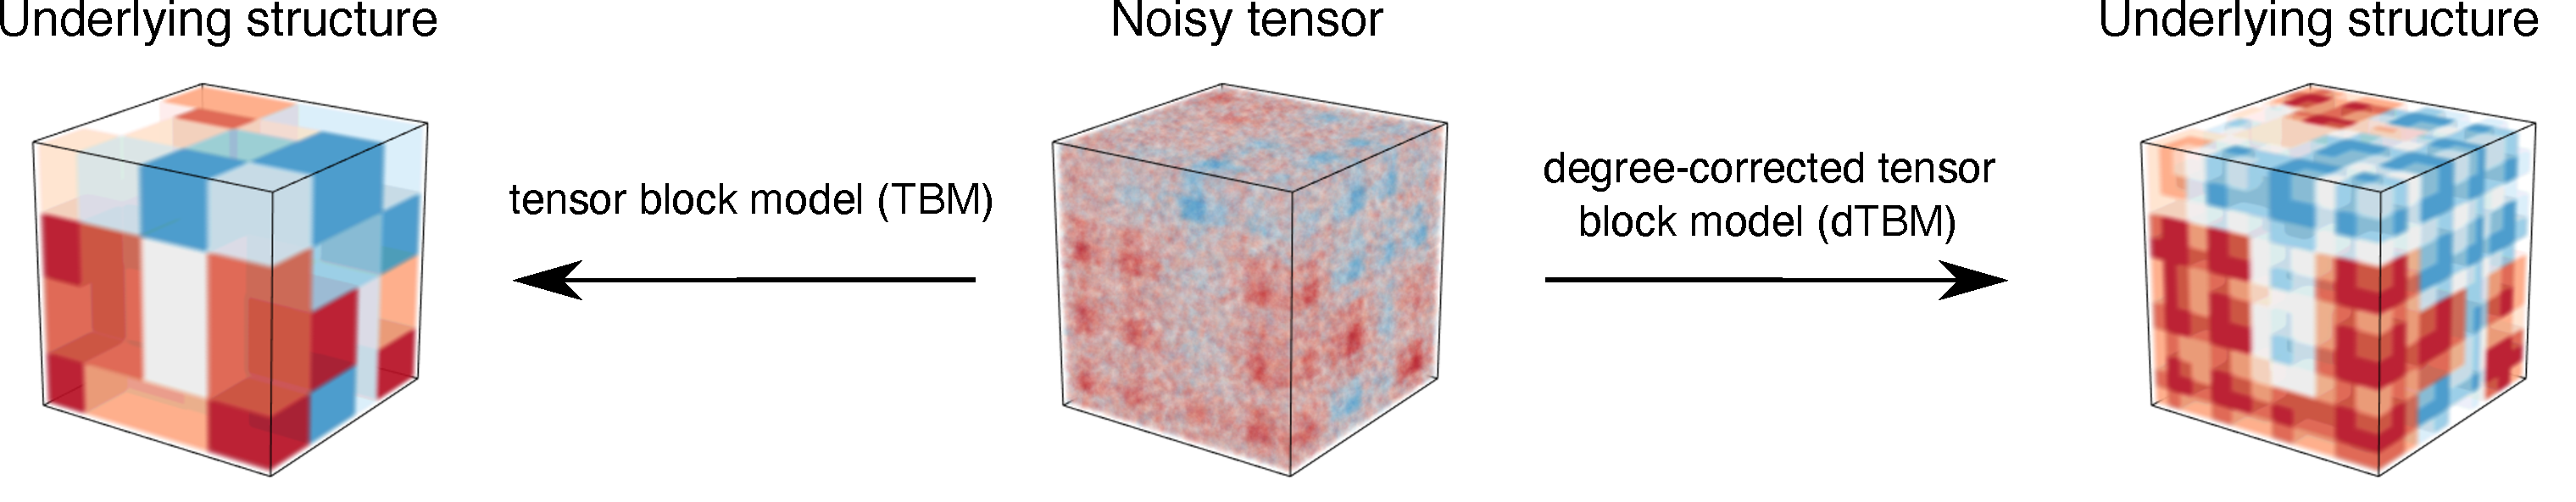
\includegraphics[width = .9\textwidth]{intro2_arxiv.pdf}
    \caption{Examples for order-3 tensor block model (TBM) with and without degree correction. Both TBM and dTBM have four communities on each mode, while dTBM allows a richer structure with degree heterogeneity.
    %DIF < \fixme{Miaoyan}{Use horizontal figure} 
    }
    \label{fig:intro}
\end{figure*}

{\bf Our contributions.} The primary goal of this paper is to provide both statistical and computational guarantees for dTBM. Our main contributions are summarized below.
\begin{itemize}[leftmargin=*]

 \item We develop a general dTBM and establish the identifiability for the uniqueness of clustering using the notion of angle \DIFdelbegin \DIFdel{seperability}\DIFdelend \DIFaddbegin \DIFadd{separability}\DIFaddend .

\item  We present the phase transition of clustering performance with respect to three different statistical and computational behaviors.  We characterize, for the first time, the critical signal-to-noise (SNR) thresholds in dTBMs, revealing the intrinsic distinctions among (vector) one-dimensional clustering, (matrix) biclustering, and (tensor) higher-order clustering. Specific SNR thresholds and algorithm \DIFdelbegin \DIFdel{behaviours }\DIFdelend \DIFaddbegin \DIFadd{behaviors }\DIFaddend are depicted in  Figure~\ref{fig:phase_axis}. 

 \item We provide an angle-based algorithm that achieves exact clustering \emph{in polynomial time} under mild conditions. Simulation and data studies demonstrate the outperformance of our algorithm compared with existing higher-order clustering algorithms. 
\end{itemize}
The last two contributions, to our best knowledge, are new to the literature of dTBMs. 
%DIF < Table~\ref{tab:comp} highlights the improvement of our methods over previous results. Our algorithm addresses higher-order tensor data with degree heterogeneity, allows either binary or continuous entries, and achieves exponentially fast rate in misclustering error. 



\begin{figure*}[t]
    \centering
    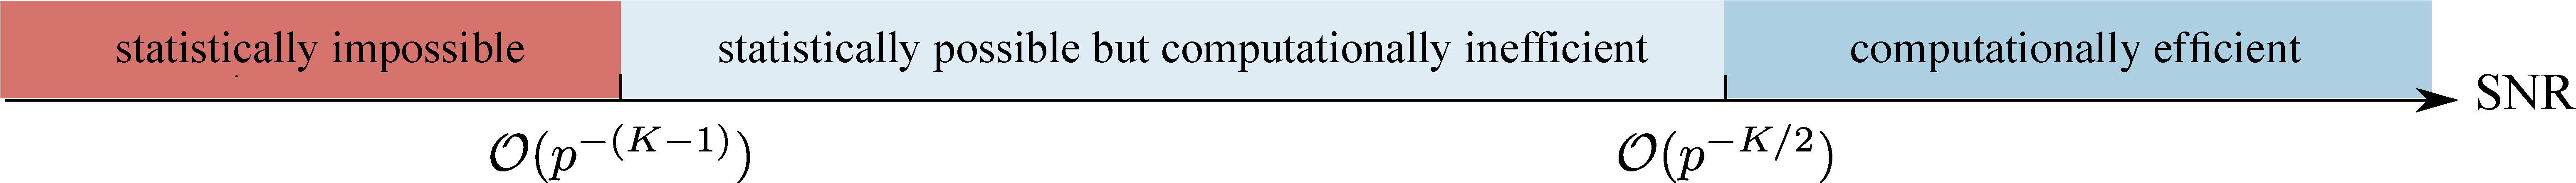
\includegraphics[width = 17cm]{phase.pdf}
    \caption{SNR thresholds for statistical and computational limits in order-$K$ dTBM with dimension $(p,...,p)$ and $K \geq 2$. The SNR gap between statistical possibility and computational efficiency  exists only for tensors with $K \geq 3$. }
    \label{fig:phase_axis}
\end{figure*}




{\bf Related work.} 
\DIFdelbegin %DIFDELCMD < {\color{blue}
%DIFDELCMD < %%%
\DIFdelend Our work is closely related to \DIFdelbegin \DIFdel{, }\DIFdelend but also distinct from several lines of existing research. \DIFaddbegin \DIFadd{Table~\ref{tab:comp} summarizes the most relevant models. 
}

\DIFaddend \begin{itemize}
    \item \textit{Block model for clustering.} Block models such as stochastic block model (SBM) and degree-corrected SBM \DIFdelbegin \DIFdel{has }\DIFdelend \DIFaddbegin \DIFadd{have }\DIFaddend been widely used for matrix clustering problems. The theoretical properties and algorithm performance for \DIFaddbegin \DIFadd{matrix }\DIFaddend block models have been well-studied\DIFaddbegin \DIFadd{~\mbox{%DIFAUXCMD
\citep{gao2018community}}\hspace{0pt}%DIFAUXCMD
}\DIFaddend ; see the review paper~\citep{abbe2017community} and the references therein. However, The tensor counterparts are relatively less understood. 
    \DIFdelbegin \DIFdel{Table~\ref{tab:comp} summarizes the most relevant models. Specifically,
    }%DIFDELCMD < \begin{itemize}
%DIFDELCMD <         %%%
\DIFdelend \DIFaddbegin 

    \DIFaddend \item  \DIFdelbegin \DIFdel{the }\DIFdelend \DIFaddbegin \textit{\DIFadd{Tensor block model.}} \DIFadd{The }\DIFaddend tensor block model (TBM, \DIFdelbegin \DIFdel{\mbox{%DIFAUXCMD
\cite{wang2019multiway, han2020exact}}\hspace{0pt}%DIFAUXCMD
) , }\DIFdelend \DIFaddbegin \DIFadd{\mbox{%DIFAUXCMD
\cite{wang2019multiway, han2020exact, ghoshdastidar2017consistency}}\hspace{0pt}%DIFAUXCMD
) is }\DIFaddend a higher-order extension of SBM, \DIFaddbegin \DIFadd{but it }\DIFaddend fails to allow degree heterogeneity. The Cartesian coordinates based analysis in \cite{han2020exact} is \DIFdelbegin \DIFdel{also }\DIFdelend non-applicable to handle the extra \DIFdelbegin \DIFdel{flexibility brought from }\DIFdelend \DIFaddbegin \DIFadd{complexity brought by degree }\DIFaddend heterogeneity. In contrast, our model addresses the degree heterogeneity, and \DIFdelbegin \DIFdel{the polar coordinates based tools are adapted }\DIFdelend \DIFaddbegin \DIFadd{we develop polar-coordinate based tools }\DIFaddend for the theoretical analysis\DIFdelbegin \DIFdel{;
        }\DIFdelend \DIFaddbegin \DIFadd{.
    }

    \DIFaddend \item \DIFdelbegin \DIFdel{the }\DIFdelend \DIFaddbegin \textit{\DIFadd{Degree-corrected block model.}} \DIFadd{The }\DIFaddend hypergraph degree-corrected block model (hDCBM) proposed by \cite{ke2019community, yuan2018testing} accounts for degree heterogeneity. \DIFdelbegin \DIFdel{Whereas}\DIFdelend \DIFaddbegin \DIFadd{However}\DIFaddend , the hDCBM is designed only for binary observations, and the proposed spectral algorithm in \cite{ke2019community} achieves \DIFdelbegin \DIFdel{a }\DIFdelend sub-optimal \DIFdelbegin \DIFdel{clustering accuracy }\DIFdelend \DIFaddbegin \DIFadd{polynomial clustering rate }\DIFaddend in higher-order scenarios. In constrast, our model allows discrete and continuous entries, and achieves \DIFdelbegin \DIFdel{exponentially }\DIFdelend \DIFaddbegin \emph{\DIFadd{exponentially}} \DIFaddend fast rate in clustering tasks. More importantly, to our best knowledge, we are the first to provide the statistical and computational limits analyses for the degree-corrected block model in tensor clustering. \DIFdelbegin %DIFDELCMD < \end{itemize}
%DIFDELCMD <     %%%
\DIFdelend \DIFaddbegin \DIFadd{See Fig~\ref{fig:phase_axis} for overview of our results. 
    }\DIFaddend 

    \item \textit{Global-to-local algorithm strategy.} Our methods generalize the recent global-to-local strategy for matrix learning~\citep{gao2018community,chi2019nonconvex,yun2016optimal} to tensors~\citep{han2020exact,ahn2018hypergraph,kim2018stochastic}. Despite the conceptual similarity, we address several fundamental challenges associated with this non-convex, non-continuous problem. We show the insufficiency of the conventional tensor HOSVD~\DIFdelbegin \DIFdel{\mbox{%DIFAUXCMD
\citep{kolda2009tensor}}\hspace{0pt}%DIFAUXCMD
}\DIFdelend \DIFaddbegin \DIFadd{\mbox{%DIFAUXCMD
\citep{de2000multilinear}}\hspace{0pt}%DIFAUXCMD
}\DIFaddend , and we develop a weighted higher-order initialization that relaxes the \DIFdelbegin \DIFdel{eigen-gap }\DIFdelend \DIFaddbegin \DIFadd{singular-value gap }\DIFaddend separation condition. Furthermore, our local iteration leverages the angle-based clustering in order to avoid explicit estimation of degree heterogeneity. Our bounds reveal the interesting interplay between the computational and statistical errors. We show that our final estimate \DIFdelbegin \DIFdel{provably }\DIFdelend \DIFaddbegin \emph{\DIFadd{provably}} \DIFaddend achieves the exact clustering within only polynomial-time complexity. 

\end{itemize}
\DIFdelbegin %DIFDELCMD < }
%DIFDELCMD < %%%
\DIFdelend 



%DIF < We emphasize the comparisons that set our work apart from earlier literature from two perspectives---models and algorithms. From the model perspective, our work extends the previous degree-corrected model from matrices to tensors. There is a huge literature on degree-corrected matrix models; see the review paper~\citep{abbe2017community} and the references therein. The tensor counterparts, however, are relatively less understood. Table~\ref{tab:comp} summarizes  the most relevant models for higher-order clustering. Earlier tensor methods either fail to allow degree heterogeneity~\citep{chien2018community,han2020exact,zhang2021exact,ghoshdastidar2017uniform,kim2018stochastic}, or suffer from sub-optimal misclustering rates~\citep{ke2019community,ghoshdastidar2017consistency,chi2020provable}. In contrast, our method addresses the degree heterogeneity, allows discrete and continuous entries, and achieves exponentially fast rate in clustering tasks.  
\DIFdelbegin %DIFDELCMD < 

%DIFDELCMD < %%%
%DIF < From the algorithm perspective, our methods generalize the recent global-to-local strategy for matrix learning~\citep{gao2018community,chi2019nonconvex,yun2016optimal} to tensors~\citep{han2020exact,ahn2018hypergraph,kim2018stochastic}. Despite the conceptual similarity, we address several fundamental challenges associated with this non-convex, non-continuous problem. We show the insufficiency of the conventional tensor HOSVD~\citep{kolda2009tensor}, and we develop a weighted higher-order initialization that relaxes the eigen-gap separation condition. Furthermore, our local iteration leverages the angle-based clustering in order to avoid explicit estimation of degree heterogeneity. Our bounds reveal the interesting interplay between the computational and statistical errors. We show that our final estimate provably achieves the exact clustering within only polynomial-time complexity. 
%DIFDELCMD < 

%DIFDELCMD < %%%
%DIF <  {
%DIF <  \color{red}
%DIFDELCMD < 

%DIFDELCMD < %%%
%DIF <  Our work is closely related to, but also distinct from several lines of existing research:
%DIF <  \begin{enumerate}
%DIFDELCMD < 

%DIFDELCMD < %%%
%DIF <  \item \textbf{Degree-corrected model.}
%DIF <      \begin{itemize}
%DIF <          \item Matrix. (1) Previous work, survey paper (2) Unique technical challenges in Tensor (3) matrix does not show statistical-computational gap;
%DIF <          \item Tensor. (Comparison with Ke) (1) Ke does not provide the SNR limits (2) Ke's algorithm is sub-optimal (3) Ke focuses on Binary data. 
%DIF <      \end{itemize}
%DIFDELCMD < 

%DIFDELCMD < %%%
%DIF <      \item \textbf{Higher-order clustering.} (1) Previous work fails to account the heterogeneity, which is not realistic; (2) The extension of theoretical results highly challenging.  Extra nuisance parameter makes it more difficult to establish the statistical and computational limits. 
    %DIFDELCMD < 

%DIFDELCMD < %%%
%DIF <      \item \textbf{Spherical clustering.} 
    %DIFDELCMD < 

%DIFDELCMD < %%%
%DIF <      \item \textbf{Global-to-local algorithm.} (1) Matrix global-to-local algorithm (2) Tensor global-to-local algorithm is used for non-degree algorithm. Extra nuisance parameter makes it necessary to consider angle-based similarity; angle-based clustering makes the Cartesian coordinates based analysis non-applicable for our setting. 
%DIF <  \end{enumerate}
%DIFDELCMD < 

%DIFDELCMD < %%%
%DIF <  }
%DIFDELCMD < 

%DIFDELCMD < %%%
\DIFdelend \begin{table*}[t]
\DIFdelbeginFL %DIFDELCMD < \resizebox{\textwidth}{!}{%
%DIFDELCMD < \color{blue}
%DIFDELCMD <     \begin{tabular}{c|ccccc}
%DIFDELCMD < \hline
%DIFDELCMD <     & \cite{gao2018community}&  \cite{han2020exact}&  \cite{ghoshdastidar2017consistency} &\cite{ke2019community} & \textbf{Ours}\\
%DIFDELCMD <     \hline
%DIFDELCMD <         {\small Allow tensors}& $\times$ & $\surd$ & $\surd$ &$\surd$ & $\surd$  \\
%DIFDELCMD <         {\small Allow heterogeneity} &  $\surd$ & $\times$ & $\surd$ &$\surd$ & $\surd$ \\
%DIFDELCMD <         %Assortative assumption&  $\surd$ & $\times$ & $\times$ & $\times$\\
%DIFDELCMD <        %{\small Allow various data} & $\times$ & $\surd$ & $\times$ & $\surd$  &$\surd$\\
%DIFDELCMD <         {\small Eigen free clustering} &  $\surd$ & $\surd$ & $\times$ & $\times$ &$\surd$ \\
%DIFDELCMD <         %{\small Misclustering rate (for order 2$^*$)}& $\exp(-p)$ & $\exp(-p)$ & $p^{-1}$ & $p^{-1}$& $\exp(-p)$\\
%DIFDELCMD <         {\small Misclustering rate (for order $K^*$)}& - & $\exp(-p^{K/2})$ & $p^{-1}$& $p^{-2}$ &  $\exp(-p^{K/2})$\\
%DIFDELCMD <         \hline
%DIFDELCMD <     \end{tabular}
%DIFDELCMD <     }
%DIFDELCMD <     %%%
\DIFdelendFL \DIFaddbeginFL \resizebox{\textwidth}{!}{%
    \begin{tabular}{c|ccccc}
\hline
    & \cite{gao2018community}&  \cite{han2020exact}&  \cite{ghoshdastidar2017consistency} &\cite{ke2019community} & \textbf{Ours}\\
    \hline
      Allow tensors of arbitrary order & $\times$ & $\surd$ & $\surd$ &$\surd$ & $\surd$  \\
        Allow degree heterogeneity &  $\surd$ & $\times$ & $\surd$ &$\surd$ & $\surd$ \\
        Singular-value gap-free clustering &  $\surd$ & $\surd$ & $\times$ & $\times$ &$\surd$ \\
        Misclustering rate (for order $K^*$)& - & $\exp(-p^{K/2})$ & $p^{-1}$& $p^{-2}$ &  $\exp(-p^{K/2})$\\
        \hline
    \end{tabular}
    }
    \DIFaddendFL \caption{Comparison between previous methods with our method. $^*$We list the result for order-K tensors with $K \geq 3$ and general number of communities $r = \tO(1)$. %DIF <  Our results allow general tensors of arbitrary order $K$; See Theorem~\ref{thm:refinement}.
    }\label{tab:comp}
\end{table*}

{\bf Notation.} We use lower-case letters (e.g., $a,b$) for scalars, lower-case boldface letters (e.g., $\ma,\mtheta$) for vectors, upper-case boldface letters (e.g., $\mX,\mY$) for matrices, and calligraphy letters (e.g., $\tX,\tY$) for tensors of order three or greater. We use \DIFaddbegin \DIFadd{$\mone_p$ to denote a vector of length $p$ with all entries to be 1. We use }\DIFaddend $|\cdot|$ for the cardinality of a set and $\ind\{\cdot\}$ for the indicator function. For an integer $p\in\mathbb{N}_{+}$, we use the shorthand $[p]= \offf{1,2,...,p}$. For a length-$p$ vector $\ma$, we use $a(i)\in\mathbb{R}$ to denote the $i$-th entry of $\ma$, and use $\ma_{I}$ to denote the sub-vector by restricting the indices in the set $I\subset [p]$.  We use  $\onorm{\ma}=\sqrt{\sum_{i}a^2(i)}$ to denote the $\ell_2$-norm, $\onorm{\ma}_1=\sum_i |a_i|$ to denote the $\ell_1$ norm of $\ma$. For two vector $\ma, \mb$ of the same dimension, we denote the angle between $\ma, \mb$ by 
\begin{equation}
    \cos \of{\ma, \mb} = \frac{\ang{ \ma, \mb}}{ \onorm{\ma} \onorm{\mb} },
\end{equation}
where $\ang{\ma,\mb}$ is the inner product of two vectors and $\cos \of{\ma, \mb} \in [-1,1]$. We make the convention that $\cos \of{\ma, \mb} = \cos \of{\ma^T, \mb^T}$. 

\DIFdelbegin \DIFdel{For a matrix $\mY$, we use $\mY_{i:}$ to  denote the $i$-th row of the matrix. }\DIFdelend Let $\tY  \in \bbR^{p_1 \times \cdots \times p_K}$ be an order-$K$ $(p_1,...,p_K)$-dimensional tensor. We use $\tY(i_1,\ldots,i_K)$ to denote the $(i_1,\ldots,i_K)$-th entry of $\tY$. The multilinear multiplication of a tensor $\tS\in \bbR^{r_1\times \cdots \times r_K}$ by matrices $\mM_k \in\mathbb{R}^{p_k\times r_k}$ results in an order-$d$ $(p_1,\ldots,p_K)$-dimensional tensor $\tX$, denoted
\[
\tX=\tS \times_1 \mM_1 \times \cdots \times_K \mM_K,
\]
where the entries of $\tX$ are defined by
\DIFdelbegin %DIFDELCMD < \begin{align}
%DIFDELCMD <     &\tX(i_1,\ldots, i_K)\\
%DIFDELCMD <     &=\sum_{(j_1,\ldots,j_K)}\tS(j_1,\ldots,j_K)\mM_1(i_1,j_1)\cdots \mM_K(i_K,j_K).
%DIFDELCMD < \end{align}%%%
\DIFdelend \DIFaddbegin \begin{align}
    &\tX(i_1,\ldots, i_K)=\sum_{(j_1,\ldots,j_K)}\tS(j_1,\ldots,j_K)\mM_1(i_1,j_1)\cdots \mM_K(i_K,j_K).
\end{align}\DIFaddend  
\DIFaddbegin \DIFadd{For a matrix $\mY$, we use $\mY_{i:}$ (respectively, $\mY_{:i}$) to denote the $i$-th row (respectively, $i$-th column) of the matrix. Similarly, for an order-3 tensor, we use $\tY_{::i}$ to denote the $i$-th matrix slide of the tensor. }\DIFaddend We use $\text{Ave}(\cdot)$ to denote the operation of taking averages across elements and $\text{Mat}_k(\cdot)$ to denote the unfolding operation that reshapes the tensor along mode $k$ into a matrix. For a symmetric tensor $\tY\in\mathbb{R}^{p\times \cdots \times p}$, we omit the subscript and use $\text{Mat}(\tY)\in\mathbb{R}^{p\times p^{K-1}}$ to denote the unfolding. For two sequences $\{a_p\}, \{b_p\}$, we denote $a_p\lesssim b_p$ \DIFaddbegin \DIFadd{or $a_p=\tO(b_p)$ if $\lim_{p\to\infty}a_p /b_p\leq c$ for some constant $c\geq 0$, $a_p=o(b_p)$ }\DIFaddend if \DIFdelbegin \DIFdel{$\lim_{p\to\infty} a_p/b_p \leq c$ }\DIFdelend \DIFaddbegin \DIFadd{$\lim_{p\to\infty}a_p/b_p =0$, }\DIFaddend and $a_p = \Omega(b_p)$ if \DIFdelbegin \DIFdel{$c b_p \leq a_p \leq C b_p$, for some constants $c, C\geq 0$}\DIFdelend \DIFaddbegin \DIFadd{both $b_p \lesssim a_p$ and $a_p\lesssim b_p$}\DIFaddend . Throughout the paper, we use the terms ``community'' and ``clusters'' exchangeably. 
%DIF < \fixme{Miaoyan}{\color{red} need to define $\cos(\ma,\mb)$. Be careful with signs.}


{\DIFdelbegin %DIFDELCMD < \color{blue}
%DIFDELCMD < 

%DIFDELCMD < {%%%
\DIFdelend \bf Organization.} The rest of this paper is organized as follows. Section~\ref{sec:model} introduces the degree-corrected tensor block model (dTBM) with three motivating examples and presents the identifiability of dTBM under the angle gap condition. We show the phase transition and the existence of statistical-computational gaps for the higher-order dTBM in Section~\ref{sec:limits}. In Section~\ref{sec:alg}, we provide a polynomial-time two-stage algorithm with misclustering rate guarantees. Numerical studies including the \DIFdelbegin \DIFdel{simulations to assess the theoretical results}\DIFdelend \DIFaddbegin \DIFadd{simulation}\DIFaddend , comparison with other methods, and \DIFdelbegin \DIFdel{real data analysis on human brain connectome data and Peru legislation data are in Section~\ref{sec:simulation}. Last, we conclude our paper }\DIFdelend \DIFaddbegin \DIFadd{two real dataset analyses are in Sections~\ref{sec:simulation}-\ref{sec:real}. The main technical ideas we develop for addressing main theorems are provided }\DIFaddend in Section~\DIFdelbegin \DIFdel{\ref{sec:con}. }\DIFdelend \DIFaddbegin \DIFadd{\ref{sec:mainproof}. Detailed proofs and extra theoretical results are provided in Appendix.
}\DIFaddend 


\DIFdelbegin %DIFDELCMD < }
%DIFDELCMD < 

%DIFDELCMD < %%%
\DIFdelend \section{Model formulation \DIFaddbegin \DIFadd{and motivations}\DIFaddend }\label{sec:model}

\subsection{Degree-corrected tensor block model}

Suppose we have an order-$K$ data tensor $\tY \in \bbR^{p \times \cdots \times p}$. For ease of notation, we focus on symmetric tensors in this section; \DIFdelbegin \DIFdel{our framework easily extends }\DIFdelend \DIFaddbegin \DIFadd{the extension }\DIFaddend to general asymmetric tensors \DIFaddbegin \DIFadd{is provided in Section~\ref{subsec:exten}}\DIFaddend . Assume there exist $r \geq 2$  disjoint communities among the $p$ nodes. We represent the community assignment by a function $z \colon [p]\mapsto[r]$, where $z(i) = a$ for $i$-th node that belongs to the $a$-th community. Then, $z^{-1}(a)=\{i\in[p]\colon z(i)=a\}$ denotes the set of nodes that belong to the $a$-th community, and $|z^{-1}(a)|$ denotes the number of nodes in the $a$-th community. %DIF < , and we let $p_a = \sum_{i \in [p]}\ind \offf{ z_i= a}$ denote the size of $a$-th community. 
Let $\mtheta=(\theta(1),\ldots,\theta(p))^T$ denote the degree heterogeneity for $p$ nodes. We consider the order-$K$ dTBM~\citep{ghoshdastidar2017consistency,ke2019community},
\begin{equation}\label{eq:model_margin}
    \tY(i_1,\ldots,i_K) = \tS(z(i_1),\ldots,z(i_K)) \prod_{k = 1}^K\theta_{i_k} + \tE(i_1,\ldots,i_K), 
\end{equation}
\normalsize
where $\tS \in \bbR^{r \times \cdots \times r}$ is an order-$K$ tensor collecting the block means among communities, and $\tE\in\mathbb{R}^{p\times \cdots \times p}$ is a noise tensor consisting of independent \DIFdelbegin \DIFdel{mean-zero }\DIFdelend \DIFaddbegin \DIFadd{zero-mean }\DIFaddend sub-Gaussian entries with variance bounded by $\sigma^2$. The unknown parameters are $z$, $S$, and $\mtheta$. The dTBM can be equivalently written in a compact form of tensor-matrix product:
\DIFdelbegin %DIFDELCMD < \begin{equation}\label{eq:model_tensor}
%DIFDELCMD <  \mathbb{E}\tY = \tS \times_1 \mTheta \mM \times_2 \cdots \times_K  \mTheta \mM,
%DIFDELCMD < \end{equation}%%%
\DIFdelend \DIFaddbegin \begin{equation}\label{eq:model_tensor}
\bbE\tY = \tS \times_1 \mTheta \mM \times_2 \cdots \times_K  \mTheta \mM,
\end{equation}\DIFaddend 
where $\mTheta = \text{diag}(\theta(1),...,\theta(p)) \in \bbR^{p \times p}$ is a diagonal matrix, $\mM \in \offf{0,1}^{p \times r}$ is the membership matrix associated with community assignment $z$ such that $\mM(i,j)=\ind\{z(i)=j\}$. By definition, each row of $\mM$ has one copy of 1's and 0's elsewhere. Note that the discrete nature of $\mM$ renders our model~\eqref{eq:model_tensor} more challenging than Tucker decomposition. %DIF < The Tucker rank of the signal tensor $\bbE \tY$ is bounded by, but not necessarily equal to, $(r,...,r)$~\citep{wang2019multiway}. 
We call a tensor $\tY$ an $r$-block tensor with degree $\mtheta$ %DIF < with the core tensor $\tS$ 
if $\tY$ admits dTBM~\eqref{eq:model_tensor}. \DIFdelbegin \DIFdel{Here, we give two special cases of dTBM. }\DIFdelend \DIFaddbegin \DIFadd{The goal of clustering is to estimate $z$ from a single noisy tensor $\tY$. We are particularly interested in the high-dimensional regime where $p$ grows whereas $r=\tO(1)$. 
}\DIFaddend 


\DIFdelbegin %DIFDELCMD < {
%DIFDELCMD < \color{blue}
%DIFDELCMD < 

%DIFDELCMD < %%%
\DIFdelend \subsection{Motivating \DIFdelbegin \DIFdel{Examples.}\DIFdelend \DIFaddbegin \DIFadd{examples}\DIFaddend } Here, we provide \DIFdelbegin \DIFdel{three }\DIFdelend \DIFaddbegin \DIFadd{four }\DIFaddend applications to illustrate the practical necessity of dTBM.

\vspace{0.2cm}
\paragraph{Tensor block model} Consider the model~\eqref{eq:model_tensor}. Let $\theta(i)=1$ for all $ i \in [p]$. The model~\eqref{eq:model_tensor} reduces to the tensor block model, which is widely used in previous clustering algorithms~\citep{wang2019multiway,chi2020provable,han2020exact}. The theoretical results in TBM serve as benchmarks for dTBM.  

\vspace{0.2cm}

\paragraph{Community detection in hypergraphs} Hypergraph network is a powerful tool to \DIFdelbegin \DIFdel{collect }\DIFdelend \DIFaddbegin \DIFadd{represent }\DIFaddend the complex entity relations with higher-order interactions~\citep{ke2019community}. A typical undirected hypergraph is denoted as $H = (V,E)$, where $V = [p]$ is the set of nodes and $E$ is the set of undirected hyperedges. Each hyperedge in $E$ is a subset of $V$, and we call the hyperedge an order-$K$ edge if the corresponding subset involves $K$ nodes. We call $H$ a $K$-uniform hypergraph if $E$ only contains order-$K$ edges. 

\DIFdelbegin \DIFdel{Similar with the adjacency matrix, it }\DIFdelend \DIFaddbegin \DIFadd{It }\DIFaddend is natural to represent the $K$-uniform hypergraph \DIFdelbegin \DIFdel{by }\DIFdelend \DIFaddbegin \DIFadd{using }\DIFaddend a binary order-$K$ adjacency tensor. Let $\tY \in \{0,1\}^{p \times \cdots \times p}$ denote the adjacency tensor, where the entries encode the presence or absence of \DIFdelbegin \DIFdel{hyperdeges }\DIFdelend \DIFaddbegin \DIFadd{order-$K$ edges }\DIFaddend among $p$ nodes. Specifically, \DIFdelbegin %DIFDELCMD < \begin{equation}
%DIFDELCMD <     \tY(i_1,...,i_K) =  \begin{cases}
%DIFDELCMD <     1  & \text{if }  (i_1,...,i_K) \in E\\
%DIFDELCMD <     0 & \text{if }  (i_1,...,i_K) \notin E
%DIFDELCMD <     \end{cases},
%DIFDELCMD < \end{equation}
%DIFDELCMD < %%%
\DIFdelend for all $(i_1,\ldots,i_K) \in [p]^K$\DIFdelbegin \DIFdel{. 
}\DIFdelend \DIFaddbegin \DIFadd{, we have
}\begin{equation}
    \tY(i_1,...,i_K) =  \begin{cases}
    1  & \text{if }  (i_1,...,i_K) \in E,\\
    0 & \text{if }  (i_1,...,i_K) \notin E.
    \end{cases}
\end{equation}
\DIFaddend 


Assume there exist $r$ disjoint communities among $p$ nodes\DIFdelbegin \DIFdel{. The }\DIFdelend \DIFaddbegin \DIFadd{, and the connection probabilities depend on the community assignments and node effects. 
Then, the }\DIFaddend equation~\eqref{eq:model_tensor} models \DIFdelbegin \DIFdel{$\mathbb{E}\tY$ }\DIFdelend \DIFaddbegin \DIFadd{$\bbE \tY$ }\DIFaddend with unknown degree heterogeneity $\mtheta$ and \DIFdelbegin \DIFdel{subgaussianity }\DIFdelend \DIFaddbegin \DIFadd{sub-Gaussianity }\DIFaddend parameter $\sigma^2 = 1/4$.  

\vspace{0.2cm}
\paragraph{Multi-layer weighted network} 
Multi-layer weighted network data consists of multiple networks \DIFdelbegin \DIFdel{with }\DIFdelend \DIFaddbegin \DIFadd{over }\DIFaddend the same set of nodes. One representative example is the brain \DIFdelbegin \DIFdel{structural }\DIFdelend connectome data~\citep{zhang2019tensor}. The multi-layer weighted network $\tY$ has dimension of $p \times p \times L$, where $p$ denotes the number of brain regions \DIFdelbegin \DIFdel{in }\DIFdelend \DIFaddbegin \DIFadd{of }\DIFaddend interest, and $L$ denotes the number of \DIFdelbegin \DIFdel{layer}\DIFdelend \DIFaddbegin \DIFadd{layers (networks)}\DIFaddend . Each of the $L$ networks describes one aspect of the brain \DIFdelbegin \DIFdel{connections, and the }\DIFdelend \DIFaddbegin \DIFadd{connectivity, such as functional connectivity or structural connectivity. The resulting }\DIFaddend tensor $\tY$ \DIFdelbegin \DIFdel{include a mixture slices with continuous, binary, and count entries}\DIFdelend \DIFaddbegin \DIFadd{consists of a mixture of slices with various data types}\DIFaddend . 


%DIF <  We use $G = (V, \{E_l\}_{l=1}^L)$ denote a $L$-layer undirected multi-layer network, where $E_l$ is the set of edges in the network of the $l$-th layer. Let $\mY_l \in \{0,1\}^{p\times p}$ denote the adjacency matrix for the $L$-th layer with nodes $V$ and edges $E_l$. Then, the multi-layer network is represented by an order-3 binary tensor $\tY \in \{0,1\}^{p \times p \times L}$, where 
%DIF <  \begin{equation}
%DIF <      \tY(i_1,i_2,l) = \mY_l(i_1,i_2),
%DIF <  \end{equation}
%DIF <  for all $(i_1,i_2) \in [p]^2$ and $l \in [L]$.
\DIFdelbegin %DIFDELCMD < 

%DIFDELCMD < %%%
\DIFdelend Assume there exist $r$ disjoint communities among $p$ nodes and $r_l$ disjoint communities among the $L$ layers. The multi-layer network community detection is modeled by the generalized asymmetric dTBM model~\eqref{eq:model_tensor}
\DIFdelbegin %DIFDELCMD < \begin{equation}
%DIFDELCMD <     \bbE[\tY] = \tS \times_1 \mTheta \mM \times_2 \mTheta \mM \times_3 \mTheta_l \mM_l, 
%DIFDELCMD < \end{equation}%%%
\DIFdelend \DIFaddbegin \begin{equation}
    \bbE \tY = \tS \times_1 \mTheta \mM \times_2 \mTheta \mM \times_3 \mTheta_l \mM_l, 
\end{equation}\DIFaddend 
where $(\mtheta \in \bbR^p, \mM \in \{0,1\}^{p \times r})$ and $ (\mtheta_l \in \bbR^L, \mM_l \in \{0,1\}^{L \times r_l})$ are the degree heterogeneity and membership matrices corresponding to the community structure for $p$ nodes and $L$ layers, respectively. 
\vspace{0.2cm}

\paragraph{Gaussian higher-order clustering} Datasets in various fields such as medical image, genetics, and computer science are formulated as Gaussian tensors. One typical example is the multi-tissue gene expression dataset, which records the different gene expression in different individuals and different tissues. The dataset, denoted as $\tY \in \bbR^{p \times n \times t}$, consists of the expression data for $p$ genes of $n$ individuals in $t$ tissues. 

Assume there exist $r_1, r_2, r_3$ disjoint clusters for $p$ genes, $n$ individuals, and $t$ tissues, respectively. We apply the generalized asymmetric dTBM model~\eqref{eq:model_tensor} 
\DIFdelbegin %DIFDELCMD < \begin{equation}
%DIFDELCMD <     \bbE[\tY] = \tS \times_1 \mTheta_1 \mM_1 \times_2 \mTheta_2 \mM_2 \times_3 \mTheta_3 \mM_3, 
%DIFDELCMD < \end{equation}%%%
\DIFdelend \DIFaddbegin \begin{equation}
    \bbE\tY = \tS \times_1 \mTheta_1 \mM_1 \times_2 \mTheta_2 \mM_2 \times_3 \mTheta_3 \mM_3, 
\end{equation}\DIFaddend 
where $\{(\mtheta_k, \mM_k)\}_{k=1}^3$ \DIFdelbegin \DIFdel{refers to }\DIFdelend \DIFaddbegin \DIFadd{represents }\DIFaddend the heterogeneity and membership for genes, individuals, and tissues. \DIFaddbegin \\
\DIFaddend 


\DIFdelbegin %DIFDELCMD < }
%DIFDELCMD < %%%
%DIF <  \begin{example}[Gaussian TBM]
%DIF <  Let $\theta(i)= 1$ for all $i \in [p]$ and $\tE$ be a noise tensor with i.i.d.\ $N(0,\sigma^2)$ entries. Our dTBM reduces to a non-degree Gaussian TBM, which is widely used in previous clustering algorithms~\citep{wang2019multiway,chi2020provable,han2020exact}. The theoretical results in TBM serve as benchmarks for dTBM. 
%DIF <  \end{example}
%DIFDELCMD < 

%DIFDELCMD < %%%
%DIF <  \begin{example}[Binary dTBM]
%DIF <  Consider a $K$-uniform hypergraph $H = (V,E)$, where $V = [p]$ collects the nodes with $r$ disjoint communities and $E$ collects all the $K$-way hyperedges. Let $\tY \in \{0,1\}^{p \times \cdots \times p}$ denote the adjacency tensor, where the entries encode the presence or absence of hyperdeges among $p$ nodes. Specifically, let $\tY(i_1,...,i_K) = 1$ if  $(i_1,...,i_K) \in E$, otherwise, $\tY(i_1,...,i_K) = 0$, for all $(i_1,\ldots,i_K) \in [p]^K$. The equation~\eqref{eq:model_tensor} models $\mathbb{E}\tY$ with unknown degree heterogeneity and subgaussianity parameter $\sigma^2 = 1/4$. 
%DIF <  \end{example}
%DIFDELCMD < 

%DIFDELCMD < %%%
\DIFdelend \begin{rmk}[Comparison with non-degree models]
Our dTBM uses fewer block parameters than TBM. \DIFdelbegin \DIFdel{Let the subscripts ``deg" and ``non" denote quantities in the models with and without degrees, respectively. Then, every $r_{\text{non}}$}\DIFdelend \DIFaddbegin \DIFadd{In particular, every non-degree $r_1$}\DIFaddend -block tensor can be represented by a \DIFdelbegin \DIFdel{degree-corrected $r_{\text{deg}}$}\DIFdelend \DIFaddbegin \emph{\DIFadd{degree-corrected}} \DIFadd{$r_2$}\DIFaddend -block tensor with \DIFdelbegin \DIFdel{$r_{\text{deg}}\leq r_{\text{non}}$}\DIFdelend \DIFaddbegin \DIFadd{$r_2\leq r_1$}\DIFaddend . In particular, there exist tensors with \DIFdelbegin \DIFdel{$r_{\text{non}}=p$ but $r_{\text{deg}}=1$}\DIFdelend \DIFaddbegin \DIFadd{$r_1=p$ but $r_2=1$}\DIFaddend , so the reduction in \DIFdelbegin \DIFdel{$r$ }\DIFdelend \DIFaddbegin \DIFadd{model complexity }\DIFaddend can be dramatic from $p$ to 1. This fact highlights the benefits of introducing degree heterogeneity in higher-order clustering tasks.
\end{rmk}


%DIF <  In addition, the following example highlights the benefits of degree correction in clustering tasks. 
%DIF <  \begin{example}[Comparison to non-degree models]\label{ex:benefit}
%DIF <  Every $r_{\text{non}}$-block tensor can be represented by degree-corrected $r_{\text{deg}}$-block tensor with $r_{\text{deg}}\leq r_{\text{non}}$. In particular, there exist tensors with $r_{\text{non}}=p$ but $r_{\text{deg}}=1$.
%DIF <  \end{example}
%DIF <  %In principle, every $(p,\ldots,p)$-dimensional tensor can be represented by a $p$-block tensor.
%DIF <  The above example shows that our dTBM uses fewer block parameters than TBM, and the reduction in $r$ can be dramatic from $p$ to 1. This fact shows the advantages of introducing degree heterogeneity in high-dimensional clustering.
\DIFdelbegin %DIFDELCMD < 

%DIFDELCMD < %%%
\DIFdelend \subsection{Identifiability under angle gap condition}
The goal of clustering is to estimate the partition function $z$ from model~\eqref{eq:model_tensor}. \DIFaddbegin \DIFadd{For ease of notation, we focus on symmetric tensors; the extension to non-symmetric tensors are similar. }\DIFaddend We use $\tP$ to denote the following parameter space for $(z,\tS,\mtheta)$,
\begin{align}\label{eq:family}
\tP=\bigg\{(z,\tS,\mtheta)\colon  \ \mtheta\in\mathbb{R}^p_{+},\ 
{c_1p\over r}\leq |z^{-1}(a)|\leq {c_2 p\over r}, c_3\leq \onormSize{}{\text{Mat}(\tS)_{a:}}\leq c_4, \onorm{\mtheta_{z^{-1}(a)}}_1=|z^{-1}(a)|, a\in[r]\bigg\},
\end{align}
\normalsize
where $c_i>0$'s are universal constants. %DIF < We briefly describe the rationale of the constraints in~\eqref{eq:family}. 
\DIFaddbegin \DIFadd{We briefly describe the rationale of the constraints in~}\eqref{eq:family}\DIFadd{. 
}\DIFaddend First, the entrywise positivity constraint on  $\mtheta\in\mathbb{R}^p_{+}$ is imposed to avoid sign ambiguity between entries in $\mtheta_{z^{-1}(a)}$ and $\tS$\DIFdelbegin %DIFDELCMD < {\color{blue} %%%
\DIFdel{and thereof allow }\DIFdelend \DIFaddbegin \DIFadd{. This constraint allows }\DIFaddend the trigonometric $\cos$ to describe the angle similarity in the \DIFdelbegin \DIFdel{following }\DIFdelend Assumption~\ref{assmp:min_gap} \DIFaddbegin \DIFadd{below }\DIFaddend and Sub-algorithm~\hyperref[alg:main]{2} in Section~\ref{sec:alg}\DIFdelbegin %DIFDELCMD < }%%%
\DIFdel{. This }\DIFdelend \DIFaddbegin \DIFadd{. Note that the positivity }\DIFaddend constraint can be achieved without sacrificing model flexibility, by using a slightly larger dimension of $\tS$ in the factorization~\eqref{eq:model_tensor}; see Example~\ref{ex:positive} \DIFaddbegin \DIFadd{below}\DIFaddend . Second, %DIF < the quantity $|z^{-1}(a)|$ denotes the number of nodes in $a$-th community. T
\DIFdelbegin \DIFdel{the }\DIFdelend \DIFaddbegin \DIFadd{recall that the quantity $|z^{-1}(a)|$ denotes the number of nodes in $a$-th community. The }\DIFaddend constants $c_1, c_2$ in the $|z^{-1}(a)|$ bound assume the roughly balanced size across $r$ communities. Third, the constants $c_3, c_4 $ in the magnitude of $\text{Mat}(\tS)_{a:}$ requires no purely zero slide in $\tS$, so the core tensor $\tS$ is not trivially reduced to \DIFaddbegin \DIFadd{a }\DIFaddend lower rank. Lastly, the $\ell_1$ normalization $\onormSize{}{\mtheta_{z^{-1}(a)}}_1=|z^{-1}(a)|$ is imposed to avoid the scalar ambiguity between $\mtheta_{z^{-1}(a)}$ and $\tS$. This constraint, again, incurs no restriction to model flexibility but makes our presentation cleaner. 

\begin{example}[Positivity of degree parameters]~\label{ex:positive}
Here we provide an example to show the positivity constraints on $\mtheta$ incurs no loss on the model flexibility. 
\DIFdelbegin %DIFDELCMD < {\color{blue}
%DIFDELCMD < %%%
\DIFdel{We consider a }\DIFdelend \DIFaddbegin \DIFadd{Consider an }\DIFaddend order-3 dTBM with core tensor $\tS = 1$ and degree $\mtheta = (1,1,-1, -1)^T$. We have the mean tensor 
\begin{equation}
    \tX = \tS \times_1 \mTheta \mM \times_2 \mTheta \mM \times_3 \mTheta \mM,
\end{equation}
where $\mTheta = \text{diag}(\mtheta)$ and $\mM = (1,1,1,1)^T$. Note that $\tX \in \bbR^{4 \times 4 \times 4}$ is a 1-block tensor with \DIFdelbegin \DIFdel{mixed-signed }\DIFdelend \DIFaddbegin \emph{\DIFadd{mixed-signed}} \DIFaddend degree $\mtheta$, and the mode-3 slices of $\tX$ are
\begin{equation}
    \tX_{::1} = \tX_{::2} = - \tX_{::3} = -\tX_{::4}  = \begin{bmatrix}
    1 & 1& -1& -1 \\
    1 & 1& -1& -1 \\
    -1& -1&1 & 1\\
     -1& -1&1 & 1
    \end{bmatrix}.
\end{equation}
Now, instead of original decomposition, we encode \DIFdelbegin \DIFdel{$\tS$ }\DIFdelend \DIFaddbegin \DIFadd{$\tX$ }\DIFaddend as a 2-block tensor with \DIFdelbegin \DIFdel{positive-signed degree}\DIFdelend \DIFaddbegin \emph{\DIFadd{positive-signed}} \DIFadd{degree. Specifically, we write
}\DIFaddend \begin{equation}
     \tX = \tS' \times_1 \mTheta' \mM' \times_2 \mTheta' \mM'  \times_3 \mTheta' \mM' , 
\end{equation}
where \DIFaddbegin \DIFadd{$\mTheta' = \text{diag}(\mtheta') = \text{diag}(1,1, 1, 1)$, the core tensor }\DIFaddend $\tS' \in \bbR^{2 \times 2 \times 2}$ \DIFdelbegin \DIFdel{have }\DIFdelend \DIFaddbegin \DIFadd{has }\DIFaddend mode-3 slices\DIFdelbegin %DIFDELCMD < \begin{equation}
%DIFDELCMD <     \tS'_{::1} = -\tS'_{::2} = \begin{bmatrix}
%DIFDELCMD <     1 & -1 \\
%DIFDELCMD <     -1 & 1
%DIFDELCMD <     \end{bmatrix}, \quad \mM' = \begin{bmatrix}
%DIFDELCMD <     \mI_2 & {\bf 0}\\
%DIFDELCMD <     {\bf 0} &  \mI_2
%DIFDELCMD <     \end{bmatrix},
%DIFDELCMD < \end{equation}
%DIFDELCMD < %%%
\DIFdel{and $\mTheta' = \text{diag}(\mtheta') = \text{diag}(1,1, 1, 1)$. }\DIFdelend \DIFaddbegin \DIFadd{, and the membership matrix $\mM'\in\{0,1\}^{2\times 4}$ defines the clustering $z'\colon[4]\to[2]$,
}\begin{equation}
    \tS'_{::1} = -\tS'_{::2} = \begin{bmatrix}
    1 & -1 \\
    -1 & 1
    \end{bmatrix}, \quad \mM' = \begin{bmatrix}
   1& 1 & 0 & 0\\
    0 &0 &  1& 1 
    \end{bmatrix}.
\end{equation}
 \DIFaddend The triplet $(z',\tS', \mtheta')$ lies in our parameter space~\eqref{eq:family}. In general, we can always reparameterize a block-$r$ tensor with mixed-signed degree using a block-$2r$ tensor with positive-signed degree. Since we \DIFdelbegin \DIFdel{assumes }\DIFdelend \DIFaddbegin \DIFadd{assume }\DIFaddend $r=\tO(1)$ throughout the paper, the splitting does not affect the error rates of our interest.\DIFdelbegin %DIFDELCMD < }
%DIFDELCMD < 

%DIFDELCMD < %%%
%DIF <  Without loss of generality, we consider the order-2 (i.e., matrix) block models. Consider a $4$-by-$4$ matrix with core matrix $\mS = 1$ and degree $\mtheta=(1,1,-1,-1)^T$. We have the mean matrix 
%DIF <  \begin{equation}
%DIF <      \mX = \mS \times_1 \mTheta \mM \times_2 \mTheta\mM = \begin{bmatrix}
%DIF <  1 & 1 & -1& -1\\
%DIF <  1 & 1 & -1& -1\\
%DIF <  -1 & -1 & 1& 1\\
%DIF <  -1 & -1 & 1& 1
%DIF <  \end{bmatrix},
%DIF <  \end{equation}
%DIF <  $ \text{with}\quad \mTheta=\text{diag}(\mtheta)$. Note that $\mX$ is a 1-block matrix with mixed-signed degree $\mtheta$. 
%DIF <  Now, instead of original decomposition, we encode $\mX$ as a $2$-block matrix with positive-signed degree,
%DIF <  \begin{equation}
%DIF <  \mX= \mS' \times_1 \mTheta' \mM \times_2 \mTheta' \mM,\quad \text{with}\quad   \mS' = \begin{bmatrix} 1 & -1 \\
%DIF <      -1 & 1
%DIF <      \end{bmatrix}
%DIF <  \end{equation}
%DIF < and $ \mTheta'=\text{diag}(\mtheta')=\text{diag}(1, 1, 1, 1)^T$, where the triplet $(z',\mS', \mtheta')$ lies in our parameter space~\eqref{eq:family}. In general, we can always reparameterize a block-$r$ tensor with mixed-signed degree using a block-$2r$ tensor with positive-signed degree. Since we assumes $r=\tO(1)$ throughout the paper, the splitting does not affect the error rates of our interest.
\DIFdelend \end{example}

We \DIFdelbegin \DIFdel{first provide the identifiablity }\DIFdelend \DIFaddbegin \DIFadd{now provide the identifiability }\DIFaddend conditions for our model before estimation procedures. When $r=1$, the decomposition~\eqref{eq:model_tensor} is always unique (up to cluster label permutation) in $\tP$, because dTBM is equivalent to the rank-1 tensor family under this case. When $r\geq 2$, the Tucker rank of signal tensor \DIFdelbegin \DIFdel{$\mathbb{E}\tY$ }\DIFdelend \DIFaddbegin \DIFadd{$\bbE\tY$ }\DIFaddend in~\eqref{eq:model_tensor} is bounded by, but not necessarily equal to, the number of blocks $r$~\citep{wang2019multiway}. Therefore, one can not apply the classical identifiability conditions for low-rank tensors to dTBM. Here, we introduce a key separation condition on the core tensor. 

\begin{assumption}[Angle gap] \label{assmp:min_gap}Let $\mS = \text{Mat}(\tS)$. Assume the minimal gap between normalized rows of $\mS$ is bounded away from zero\DIFdelbegin \DIFdel{, }\DIFdelend \DIFaddbegin \DIFadd{; }\DIFaddend i.e.,
\DIFdelbegin %DIFDELCMD < \begin{equation}\label{eq:minimal_gap}
%DIFDELCMD <     \Delta_{\min} := \min_{a \neq b \in [r]} \onorm{\frac{\mS_{a:}}{\onormSize{}{ \mS_{a:}}} - \frac{\mS_{b:}}{\onormSize{}{ \mS_{b:}}} }>0, \quad \text{for} \quad r \geq 2,
%DIFDELCMD < \end{equation}%%%
\DIFdelend \DIFaddbegin \begin{equation}\label{eq:minimal_gap}
    \Delta_{\min} := \min_{a \neq b \in [r]} \onorm{\frac{\mS_{a:}}{\onormSize{}{ \mS_{a:}}} - \frac{\mS_{b:}}{\onormSize{}{ \mS_{b:}}} }>0, \quad \text{for} \quad r \geq 2.
\end{equation}\DIFaddend 
\DIFdelbegin \DIFdel{and set }\DIFdelend \DIFaddbegin \end{assumption}
\DIFadd{We make }\DIFaddend the convention $\Delta_{\min} = 1$ for $r = 1$. Equivalently, \DIFaddbegin \eqref{eq:minimal_gap} \DIFadd{says that }\DIFaddend none of the two rows in $\mS$ are parallel\DIFdelbegin \DIFdel{, }\DIFdelend \DIFaddbegin \DIFadd{; }\DIFaddend i.e., \DIFdelbegin \DIFdel{when $r \geq 2$, $ \max_{a \neq b\in [r]}\cos \of{\mS_{a:},\  \mS_{b:}}  = 1-\Delta^2_{\min}/2<1$. }%DIFDELCMD < \end{assumption}
%DIFDELCMD < %%%
\DIFdelend \DIFaddbegin \DIFadd{$\max_{a \neq b\in [r]}\cos \of{\mS_{a:},\  \mS_{b:}}  = 1-\Delta^2_{\min}/2<1$. }\DIFaddend The quantity $\Delta_{\min}$ characterizes the non-redundancy among clusters measured by angle separation. The \DIFaddbegin \DIFadd{denominators involved in }\DIFaddend definition~\eqref{eq:minimal_gap} \DIFdelbegin \DIFdel{is }\DIFdelend \DIFaddbegin \DIFadd{are }\DIFaddend well posed because of the lower bound on $\onorm{\mS_{a:}}$ in~\eqref{eq:family}. 
\DIFdelbegin \DIFdel{The following theorem shows that the }\DIFdelend \DIFaddbegin 

\DIFadd{Our first main result is the following theorem showing the sufficiency and necessarily of the }\DIFaddend angle gap separation \DIFdelbegin \DIFdel{is sufficient and necessary for }\DIFdelend \DIFaddbegin \DIFadd{condition for the }\DIFaddend parameter identifiability under dTBM. 

\DIFdelbegin %DIFDELCMD < \begin{thm}[Identifiability]%%%
\DIFdelend \DIFaddbegin \begin{thm}[Model identifiability]\DIFaddend \label{thm:unique} Consider the dTBM with $r\geq 2$. The parameterization~\eqref{eq:model_tensor} is unique in $\tP$ up to cluster label permutations, if and only if Assumption~\ref{assmp:min_gap} holds.
\end{thm}

The identifiability guarantee for the dTBM is more appealing than classical Tucker model. In the Tucker model, the factor matrix $\mM$ is identifiable only up to orthogonal rotations. In contrast, our model does not suffer from rotational invariance. As we will show in Section~\ref{sec:alg}, each column of the membership matrix $\mM$ can be precisely recovered under our algorithm. This property benefits the interpretation of dTBM in practice. 

\section{Statistical-computational \DIFdelbegin \DIFdel{gaps }\DIFdelend \DIFaddbegin \DIFadd{limits }\DIFaddend for higher-order tensors}\label{sec:limits}

In this section, we study the statistical and computational limits of dTBM. We \DIFdelbegin \DIFdel{reserve the term higher-order tensors for tensors of order $K\geq 3$. We }\DIFdelend propose signal-to-noise ratio~(SNR),
\begin{align}\label{eq:gamma}
  \text{SNR}:= \Delta^2_{\min}/\sigma^2 = p^{\gamma}, 
\end{align}
with varying $\gamma \in \bbR$ that quantifies different regimes of interest. We call $\gamma$ the \emph{signal exponent}. Intuitively, a larger SNR, or equivalently a larger $\gamma$, benefits the clustering in the presence of noise. With quantification~\eqref{eq:gamma}, we consider the following parameter space,
\begin{equation}\label{eq:gammafamily}
    \tP(\gamma) = \tP\cap\{\tS \text{ satisfies SNR condition~\eqref{eq:gamma} with $\gamma$} \}.
\end{equation}
Note that $1$-block dTBM does not belong to the space $\tP(\gamma)$ when $\gamma < 0$ by Assumption~\ref{assmp:min_gap}. Our goal is to characterize the clustering accuracy with respect to $\gamma$\DIFdelbegin \DIFdel{when $r \geq 2$}\DIFdelend . Let $\hat z$ and $z$ be \DIFaddbegin \DIFadd{the }\DIFaddend estimated and true clustering functions in the family~\eqref{eq:family}. Define the misclustering error by
\[
\ell(\hat z, z)={1\over p}\min_{\pi \in \Pi}\sum_{i\in[p]}\ind\{\hat z(i)\neq \pi \circ z(i)\},
\]
where $\pi: [r] \mapsto [r]$ is a permutation of cluster labels, $\circ$ denotes the composition operation, and $\Pi$ denotes the collection of all possible permutations. The infinitum over all permutations accounts for the ambiguity in cluster label permutation. 

In Sections~\ref{sec:statlimit} and \ref{sec:complimit}, we provide the lower bounds of $\ell (\hat z, z)$ for general Gaussian dTBMs\DIFaddbegin \DIFadd{~}\eqref{eq:model_margin} \DIFaddend without symmetric assumptions. For general (asymmetric) \DIFaddbegin \DIFadd{Gaussian }\DIFaddend dTBMs, we \DIFaddbegin \DIFadd{assume Gaussian noise $\tE(i_1,\ldots,i_K)\stackrel{\text{i.i.d.}}{\sim} N(0,\sigma^2)$, and we }\DIFaddend extend the parameter space~\eqref{eq:family} to allow $K$ clustering functions $(z_k)_{k\in[K]}$, one for each mode. For notational simplicity, we still use $z$ and $\tP(\gamma)$ for this general (asymmetric) model. All lower bounds should be interpreted as the worst-case results across $K$ modes. 


%DIF < For technical simplicity, we will present our main theory with a focus on Gaussian tensors. Our algorithm and comparison extend to general sub-Gaussian models with little modification. 
\DIFdelbegin %DIFDELCMD < 

%DIFDELCMD < %%%
\DIFdelend \subsection{Statistical critical values}\label{sec:statlimit}
\DIFdelbegin \DIFdel{Our first main result is to show }\DIFdelend \DIFaddbegin \DIFadd{The statistical limit means the minimal SNR required for solving dTBMs with }\emph{\DIFadd{unlimited computational cost.}} \DIFadd{Our following result shows }\DIFaddend the minimax lower bound of SNR for exact recovery in dTBM. 
%DIF < We call a dTBM general if no symmetric assumption is imposed to the signal tensor. 
\DIFaddbegin 

\DIFaddend \begin{thm}[Statistical lower bound]\label{thm:stats} Consider general Gaussian dTBMs under the parameter space $\tP(\gamma)$ with $K\geq 1$. Assume $r \lesssim p^{1/3}$. If the signal exponent satisfies $\gamma < -(K-1)$, then, every estimator $\hat z_{\text{stat}}$ obeys
\begin{equation}
    \sup_{(z, \tS, \mtheta) \in \tP(\gamma)} \bbE \left[ p\ell(\hat z_{\text{stat}}, z) \right]\geq 1.
\end{equation}
\end{thm}
Theorem~\ref{thm:stats} demonstrates the impossibility of exact recovery of the assignment when $\gamma < -(K-1)$ in the high-dimensional regime $p\to \infty$ for fixed $r$. The proof is information-theoretical, and therefore the results apply to all statistical estimators, including but not limited to, maximum likelihood estimation (MLE)~\citep{wang2019multiway} and trace maximization~\citep{ghoshdastidar2017uniform}. \DIFdelbegin \DIFdel{Our derived }\DIFdelend \DIFaddbegin \DIFadd{As we will show in Section~\ref{sec:alg}, the }\DIFaddend SNR threshold $-(K-1)$ is also a minimax upper bound, because MLE achieves exact recovery when $\gamma > -(K-1)$. Hence, the boundary $\gamma_{\text{stat}} \coloneqq -(K-1)$ is the critical value for statistical performance of dTBM. 


\subsection{Computational critical values}\label{sec:complimit}
\DIFaddbegin \DIFadd{In this section, we derive the computational limits of dTBMs. The computational limit means the minimal SNR required for exactly recovery with }\emph{\DIFadd{polynomial-time}} \DIFadd{computational cost. }\DIFaddend An important ingredient to establish the computational limits is the \emph{hypergraphic planted clique (HPC) conjecture} \citep{zhang2018tensor, brennan2020reducibility}. The HPC conjecture indicates the impossibility of fully recovering the planted cliques with polynomial-time algorithm when the clique size is less than the number of vertices in the hypergraph. %DIF < \fixme{Miaoyan}{Is this condition used in our Theorem 3?}. 
The formal statement of HPC detection \DIFdelbegin \DIFdel{and conjecture can be found }\DIFdelend \DIFaddbegin \DIFadd{conjecture is provided }\DIFaddend in Definition~\ref{def:HPC} and Conjecture~\ref{hypo:HPC} as \DIFdelbegin \DIFdel{following}\DIFdelend \DIFaddbegin \DIFadd{follows}\DIFaddend .  


\begin{defn}[Hypergraphic planted clique (HPC) detection]~\label{def:HPC} Consider an order-$K$ hypergraph $H = (V,E)$ where $V = [p]$ collects vertices and $E$ collects all the \DIFaddbegin \DIFadd{order-}\DIFaddend $K$ \DIFdelbegin \DIFdel{-way }\DIFdelend edges. Let $\tH_k(p, 1/2)$ denote the Erd\H{o}s-R\'{e}nyi $K$-hypergraph where the edge $(i_1,\ldots, i_K)$ belongs to $E$ with probability $1/2$. Further, we let $\tH_K(p, 1/2, \kappa)$ denote the hyhpergraph with planted cliques of size $\kappa$. Specifically, we generate a hypergraph from $\tH_k(p, 1/2)$, pick $\kappa$ vertices uniformly from $[p]$, denoted $K$, and then connect all the hyperedges with vertices in $K$. Note that the clique size $\kappa$ can be a function of $p$, denoted $\kappa_p$. \DIFdelbegin %DIFDELCMD < 

%DIFDELCMD < %%%
\DIFdelend The order-$K$ HPC detection aims to identify whether there exists a planted clique hidden in \DIFdelbegin \DIFdel{a }\DIFdelend \DIFaddbegin \DIFadd{an }\DIFaddend Erd\H{o}s-R\'{e}nyi $K$-hypergraph. \DIFdelbegin \DIFdel{We formulate HPC detection }\DIFdelend \DIFaddbegin \DIFadd{The HPC detection is formulated }\DIFaddend as the following hypothesis testing problem
\begin{equation}
    H_0:\ H \sim \tH_K(p,1/2) \quad \text{versus} \quad H_1: \ H \sim \tH_K(p,1/2, \kappa_p).
\end{equation}
\end{defn}

\DIFdelbegin %DIFDELCMD < \begin{conjecture}[Hypergraphic planted clique (HPC) conjecture]%%%
\DIFdelend \DIFaddbegin \begin{conjecture}[HPC conjecture]\DIFaddend \label{hypo:HPC} Consider the HPC detection problem in Definition~\ref{def:HPC}. Suppose the sequence $\{\kappa_p\}$ such that $\limsup_{p \rightarrow \infty} \log \kappa_p/ \log \sqrt{p} \leq (1 - \tau)$. Then, for \DIFdelbegin \DIFdel{any sequence of polynomial-times }\DIFdelend \DIFaddbegin \DIFadd{every sequence of polynomial-time }\DIFaddend test $\{ \varphi_p\}: H \mapsto \{0,1\}$ we have 
\begin{equation}
    \liminf_{p \rightarrow \infty} \bbP_{H_0} \of{ \varphi_p(H) =1 } +  \bbP_{H_1} \of{ \varphi_p(H) =0} \geq \frac{1}{2}.
\end{equation}
\end{conjecture}

Under the HPC conjecture, we establish the SNR lower bound that is necessary for any \emph{polynomial-time} estimator to achieve exact clustering.

\begin{thm}[Computational lower bound]\label{thm:comp} Consider general Gaussian dTBMs under the parameter space $\tP(\gamma)$ with $K\geq 2$. Assume HPC conjecture holds. If the signal exponent $\gamma < -K/2$, then, every \emph{polynomial-time estimator} $\hat z_{\text{comp}}$ obeys
\begin{align}
   \liminf_{p\to \infty}\sup_{(z, \tS, \mtheta) \in \tP(\gamma)}  \bbE \left[ p\ell(\hat z_{\text{comp}}, z) \right]\geq 1.
\end{align}
\end{thm}
Theorem~\ref{thm:comp} indicates the impossibility of exact recovery by polynomial-time algorithms when $\gamma < -K/2$.  Therefore, $\gamma_{\text{comp}}:=-K/2$ is the critical value for computational performance of dTBM.  In Section~\ref{sec:alg}, we will show the condition $\gamma> -K/2$ suffices for our proposed polynomial-time estimator. Thus, $\gamma_{\text{comp}}:=-K/2$ is the critical value for computational performance of dTBM.  

\begin{rmk}[Statistical-computational gaps]
Now, we have established the phase transition of exact clustering under order-$K$ dTBM \DIFaddbegin \DIFadd{by }\DIFaddend combing Theorems~\ref{thm:stats} and \ref{thm:comp}. Figure~\ref{fig:phase_axis} summarizes our results of critical SNRs when $K \geq 2$. \DIFaddbegin \DIFadd{In the weak SNR region $\gamma < -(K-1)$, no statistical estimator succeeds in degree-corrected higher-order clustering. In the strong SNR region $\gamma  > -K/2$, our proposed algorithm precisely recovers the clustering in polynomial time. In the moderate SNR regime, $-(K-1)\leq \gamma \leq -K/2$, the degree-corrected clustering problem is statistically easy but computationally hard. }\DIFaddend Particularly, dTBM reduces to matrix degree-corrected model when $K =2$, and the statistical and computational bounds show the same critical value. When $K =1$, dTBM reduces to the degree-corrected sub-Gaussian mixture model (GMM) with model
\begin{equation}
    \mY = \mTheta \mM \mS + \mE,
\end{equation}
where $\mY \in \bbR^{p \times d}$ collects $n$ data points in $\bbR^d$, $\mS \in \bbR^{r \times d}$ collects the $d$-dimensional centroids for $r$ clusters, and $\mTheta \in \bbR^{p \times p}, \mM \in \{0,1\}^{p \times r}, \mE \in \bbR^{p \times d}$ have the same meaning as in dTBM. \cite{lu2016statistical} implies \DIFdelbegin \DIFdel{polynomial-times }\DIFdelend \DIFaddbegin \DIFadd{that polynomial-time }\DIFaddend algorithms are able to achieve the statistical minimax lower bound in GMM. Therefore, we conclude that the statistical-to-computational gap emerges only for higher-order tensors with $K \geq 3$. The result reveals the intrinsic distinctions among (vector) one-dimensional clustering, (matrix) biclustering, and (tensor) higher-order clustering. 
\end{rmk}


%DIF < \fixme{Miaoyan}{What happens when $K=1$??} \textcolor{blue}{In our context, when $K=1$ the core tensor $\tS$ reduces to a vector and thus $\Delta_{\min}^2 = 0$. \fixme{Miaoyan}{Not correct. When $K=1$, our model reduces to Gaussian mixture models $\tY=\tS\mM\mTheta$ with $\tS\in\mathbb{R}^{r\times p}$, unknown membership matrix is $\mM\times\{0,1\}^{p\times n}$, and data $\tY\in\mathbb{R}^{n\times p}$. The goal is to cluster $n$ vectors into $r$ clusters, all in dimension $\bbR^p$. Add a remark. citep earlier work about (lack of) stat-comp gap.} } \textcolor{red}{\cite{lu2016statistical} implies there does not exist a statistical-computational bound for non-degree corrected gaussian mixture model. can replace this reference if find a reference for degree-corrected cmm.}
\DIFdelbegin %DIFDELCMD < 

%DIFDELCMD < %%%
\DIFdelend \begin{rmk}[Comparison with non-degree models]
We compare our results to non-degree tensor models. %DIF < Our parameter space of interest consists of discrete structure (for $z$) and continuous structure (for $\tS$ and $\mtheta$). 
The allowance of degree heterogeneity $\mtheta$ makes the model more flexible, but it incurs extra statistical and computational complexity. Fortunately, we find that the extra complexity does not render the estimation of $z$ qualitatively harder; see the comparison of our phase transition with non-degree TBM~\citep{han2020exact}. 
%DIF < In next section, we will supplement the general theory by providing an efficient algorithm that achieves empirical accuracy in the presence of unknown degree heterogeneity.
\end{rmk}



%DIF < \subsection{Comparison with non-degree models}
\DIFdelbegin %DIFDELCMD < 

%DIFDELCMD < %%%
%DIF <  We have established the phase transition of exact clustering under dTBM. Figure~\ref{fig:phase_axis} summarizes our results about the critical SNRs. In the weak SNR region $\gamma < -(K-1)$, no statistical estimator succeeds in degree-corrected higher-order clustering. In the strong SNR region $\gamma  > -K/2$, our proposed algorithm precisely recovers the clustering in polynomial time. In the moderate SNR regime, $-(K-1)\leq \gamma \leq -K/2$, the degree-corrected clustering problem is statistically easy but computationally hard. 
%DIF <  We find that the statistical-to-computational gap emerges only for higher-order tensors with $K \geq 3$. The result reveals the intrinsic distinctions between  (matrix) biclustering and (tensor) higher-order clustering. 
%DIFDELCMD < 

%DIFDELCMD < %%%
%DIF <  We compare our results to non-degree tensor models. Our parameter space of interest consists of discrete structure (for $z$) and continuous structure (for $\tS$ and $\mtheta$). The allowance of degree heterogeneity $\mtheta$ makes the model more flexible, but it incurs extra statistical and computational complexity. Fortunately, we find that the extra complexity does not render the estimation of $z$ qualitatively harder; see the comparison of our phase transition with non-degree TBM~\citep{han2020exact}. In next section, we will supplement the general theory by providing an efficient algorithm that achieves empirical accuracy in the presence of unknown degree heterogeneity. 
%DIFDELCMD < 

%DIFDELCMD < %%%
\DIFdelend \section{Polynomial-time algorithm under mild SNR}\label{sec:alg}
\DIFdelbegin \DIFdel{We present a two-stage clustering algorithm }\DIFdelend \DIFaddbegin \DIFadd{In this section, we present an efficient polynomial-time clustering algorithm under mild SNR}\DIFaddend . The procedure takes a global-to-local approach. See Figure~\ref{fig:demo} for illustration. The global step finds the basin of attraction with polynomial miclustering error, whereas the local iterations improve the initial clustering to exact recovery. Both steps are critical to obtain a satisfactory algorithm output. \DIFdelbegin %DIFDELCMD < {\color{blue} %%%
\DIFdel{In this section}\DIFdelend \DIFaddbegin \DIFadd{In what follows}\DIFaddend , we first use the symmetric tensor as a working example to describe the algorithm procedures to gain insight. Our theoretical analysis focuses on the noisy tensor with i.i.d.\ sub-Gaussian noise such as Gaussian and uniform observations. The extensions for asymmetric tensor and Bernoulli observation and other practical issues are in \DIFdelbegin \DIFdel{subsection}\DIFdelend \DIFaddbegin \DIFadd{Section}\DIFaddend ~\ref{subsec:exten}.
\DIFdelbegin %DIFDELCMD < }
%DIFDELCMD < %%%
\DIFdelend 

\DIFdelbegin %DIFDELCMD < \begin{figure}[t]
%DIFDELCMD < %%%
\DIFdelendFL \DIFaddbeginFL \begin{figure}[ht!]
\DIFaddendFL \centering
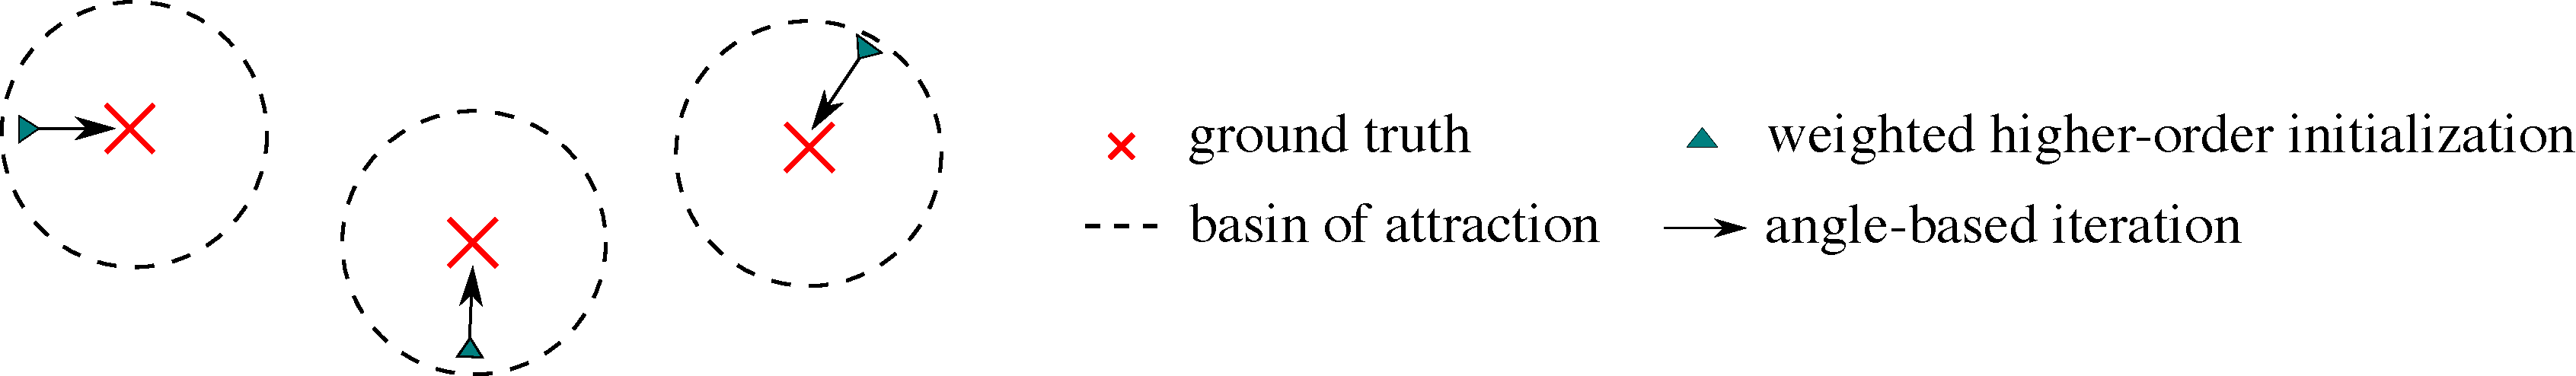
\includegraphics[width=\columnwidth]{alg_demo1.pdf}
\caption{Illustration of our global-to-local algorithm.}\label{fig:demo}
\end{figure}

\subsection{Weighted higher-order initialization}

We start with weighted higher-order clustering algorithm as initialization. \DIFdelbegin %DIFDELCMD < {\color{blue} %%%
\DIFdel{We take the }\DIFdelend \DIFaddbegin \DIFadd{We take an }\DIFaddend order-3 \DIFdelbegin \DIFdel{tensor in illustration for simplicity. }%DIFDELCMD < }  %%%
\DIFdelend \DIFaddbegin \DIFadd{symmetric tensor as illustration for insight. }\DIFaddend Consider noiseless case with $\tX = \bbE\tY$ and $\mX = \text{Mat}(\tX)$. 
By model~\eqref{eq:model_tensor}, for all $i \in [p]$, we have
\begin{equation}\label{eq:kmeans}
    \theta(i)^{-1} \mX_{i:} = \off{\text{Mat}( \tS \times_2 \mTheta \mM \times_3  \mTheta \mM )}_{z(i):}. 
\end{equation}
This implies that, all node $i$ belonging to $a$-th community (i.e., $z(i)=a$) share the same normalized mean vector $\theta(i)^{-1} \mX_{i:}$, and vice versa. Intuitively, one can apply $k$-means clustering to the vectors $\{ \theta(i)^{-1} \mX_{i:} \}_{i\in[p]}$, which leads to main idea of our Sub-algorithm~\hyperref[alg:main]{1}.  


Specifically, our initialization consists of denoising step and clustering step. The denoising step (lines 1-2 in Sub-algorithm~\hyperref[alg:main]{1}) estimates $\tX$ from $\tY$ by a double projection spectral method.  
\DIFdelbegin %DIFDELCMD < {\color{blue}
%DIFDELCMD < %%%
\DIFdelend The first projection performs HOSVD~\citep{de2000multilinear} via $\mU_{\text{pre}} = \text{SVD}_{r} \of{ \text{Mat}(\tY) }$, where $\text{SVD}_r(\cdot)$ returns the top-$r$ left singular vectors. The second projection performs HOSVD on the projected $\tY$ onto the \DIFdelbegin \DIFdel{multlilinear }\DIFdelend \DIFaddbegin \DIFadd{multilinear }\DIFaddend Kronecker space $\mU_{\text{pre}} \otimes  \mU_{\text{pre}}$; i.e.,
\DIFdelbegin %DIFDELCMD < \begin{equation}\label{eq:two-step_factor}
%DIFDELCMD <     \hat \mU = \text{SVD}_{r} \of{\text{Mat}\of{ \tY\times_1  \mU_{\text{pre}}^T \times_2  \mU_{\text{pre}}^T }}.
%DIFDELCMD < \end{equation}%%%
\DIFdelend \DIFaddbegin \begin{equation}\label{eq:two-step_factor}
    \hat \mU = \text{SVD}_{r} \of{\text{Mat}\of{ \tY\times_1  \mU_{\text{pre}} \mU_{\text{pre}}^T \times_2   \mU_{\text{pre}} \mU_{\text{pre}}^T }}.
\end{equation}\DIFaddend 
The final denoised tensor $\hat \tX$ is defined by
\begin{equation}\label{eq:two-step_est}
    \hat \tX = \tY \times_1 \hat \mU \hat 
\mU^T \times_2 \hat \mU \hat \mU^T \times_3 \hat \mU \hat \mU^T. 
\end{equation}
%DIF < Compared with conventional HOSVD, our double projection spectral method is shown to improve the estimation substantially for higher-order tensors~\citep{han2020exact}. 
The double projection improves usual matrix spectral methods in order to alleviate the noise \DIFdelbegin \DIFdel{tensor}\DIFdelend \DIFaddbegin \DIFadd{effects for $K\geq 3$~\mbox{%DIFAUXCMD
\citep{han2020exact}}\hspace{0pt}%DIFAUXCMD
}\DIFaddend .

\DIFdelbegin %DIFDELCMD < }
%DIFDELCMD < 

%DIFDELCMD < %%%
\DIFdelend The clustering step (lines 3-5 in Sub-algorithm~\hyperref[alg:main]{1}) performs the weighted $k$-means clustering. 
\DIFdelbegin %DIFDELCMD < {
%DIFDELCMD < \color{blue}
%DIFDELCMD < %%%
\DIFdelend We write $\hat \mX=\text{Mat}(\hat \tX)$, and normalize the rows into $\hat \mX^s_{i:}=\onormSize{}{\hat \mX_{i:}}^{-1}\hat \mX_{i:}$ as a surrogate of $\theta(i)^{-1} \mX_{i:}$. Then, a weighted $k$-means clustering is performed on the normalized rows with weights equal to $\onormSize{}{\hat \mX_{i:}}^2$. \DIFdelbegin %DIFDELCMD < }
%DIFDELCMD < %%%
\DIFdelend The choice of weights is to bound the $k$-means objective function by the Frobenius-norm accuracy of $\hat \tX$. Unlike existing clustering algorithm~\citep{ke2019community}, we apply the clustering on the unfolded tensor $\hat \mX$ rather than on the factors $\hat \mU$. This strategy relaxes the \DIFdelbegin \DIFdel{eigen-gap separation }\DIFdelend \DIFaddbegin \DIFadd{singular-value gap }\DIFaddend condition~\citep{gao2018community, han2020exact}.
\DIFdelbegin %DIFDELCMD < {
%DIFDELCMD < \color{blue}
%DIFDELCMD < %%%
\DIFdelend We assign degenerate rows with purely zero entries to an arbitrarily random cluster; these nodes are negligible in high-dimensions because of the lower bound on $\onormSize{}{\text{Mat}(\tS)_{a:}}$ in~\eqref{eq:family}. The final result gives the initial \DIFdelbegin \DIFdel{clustering }\DIFdelend \DIFaddbegin \DIFadd{cluster }\DIFaddend assignment $\hat z^{(0)}$. \DIFdelbegin %DIFDELCMD < }
%DIFDELCMD < %%%
\DIFdelend Full procedures are provided in Sub-algorithm~\hyperref[alg:main]{1}. 



\DIFdelbegin \DIFdel{We now establish the misclustering error rate of initialization. We call $\mtheta$ is balanced, if the relative extent of heterogeneity is comparable across clusters in that
}%DIFDELCMD < \begin{equation}\label{eq:degree}
%DIFDELCMD < {\min_{a\in[r]} \onormSize{}{\mtheta_{z^{-1}(a)}}=\left(1+o(1)\right)\max_{a\in[r]}\onormSize{}{\mtheta_{z^{-1}(a)}}}.
%DIFDELCMD < \end{equation}
%DIFDELCMD < %%%
\DIFdel{Note that, the assumption~}%DIFDELCMD < \eqref{eq:degree} %%%
\DIFdel{does not preclude degree heterogeneity. Indeed, within each of the clusters, the highest degree can be $\theta(i) = \Omega(p)$, whereas the lowest degree can be $\theta(i)=\tO(1)$. 
%DIF < instead, we assume the relative extent of heterogeneity is comparable across clusters.
}%DIFDELCMD < 

%DIFDELCMD < %%%
\DIFdelend \begin{algorithm}[h!]
\caption*{\bf Algorithm: Multiway spherical clustering for degree-corrected tensor block model }
\vspace{.15cm}
\begin{algorithmic}[1]
\Algphase{Sub-algorithm 1: Weighted higher-order initialization}
\INPUT Observation $\tY \in \bbR^{p\times \cdots \times p}$, number of \DIFdelbegin \DIFdel{cluster }\DIFdelend \DIFaddbegin \DIFadd{clusters }\DIFaddend $r$, relaxation factor $\eta > 1$ in $k$-means clustering.
\State Compute factor matrix $ \mU_{\text{pre}} = \text{SVD}_{r} (\text{Mat}(\tY))$ and the $(K-1)$-mode projection \DIFdelbegin \DIFdel{$
\tX_{\text{pre}} = \tY \times_1  \mU_{\text{pre}}^T \times_2 \cdots \times_{K-1} \mU_{\text{pre}}^T.$
}\DIFdelend \DIFaddbegin \DIFadd{$
\tX_{\text{pre}} = \tY \times_1   \mU_{\text{pre}} \mU_{\text{pre}}^T \times_2 \cdots \times_{K-1}  \mU_{\text{pre}} \mU_{\text{pre}}^T.$
}\DIFaddend \State Compute factor matrix $\hat \mU = \text{SVD}_{r}(\text{Mat}(\tX_{\text{pre}}))$ and denoised tensor
$\hat \tX = \tY \times_1 \hat \mU \hat \mU^T \times_2 \cdots \times_K \hat \mU \hat \mU^T.$
\State {Let $\hat \mX = \text{Mat}(\hat \tX)$ and $S_0=\{i \in [p]: \onormSize{}{\hat \mX_{i:}} = 0\}$. Set $\hat z(i)$ randomly in $[r]$ for $i \in S_0$.}
\State{For all $i\in S_0^c$, compute normalized rows
$\hat \mX_{i:}^s :=\onormSize{}{\hat \mX_{i:}}^{-1} \hat \mX_{i:}.$
}
\State {Solve the clustering $\hat z\colon [p]\to[r]$ and centroids $ (\hat \mx_j)_{j\in[r_k]}$ using weighted $k$-means, such that}
\begin{align}
    &\sum_{i \in S_0^c }  \onormSize{}{\hat \mX_{i:}}^2 \onormSize{}{\hat \mX_{i:}^s - \hat \mx_{\hat z(i)} }^2 
    \leq 
    \eta \min_{\substack{\bar \mx_j, j\in[r], \bar z(i),i\in S_0^{c}}} \sum_{i \in S^c } \onormSize{}{\hat \mX_{i:}}^2 \onormSize{}{ \hat \mX_{i:}^s -   \bar \mx_{\bar z(i)}}^2.
\end{align}
\OUTPUT Initial clustering $z^{(0)} \leftarrow \hat z$.

\Algphase{Sub-algorithm 2: Angle-based iteration}
%DIF < \caption{Angle-based iteration}\label{alg:refinement}
\INPUT Observation $\tY \in \bbR^{p \times \cdots \times p}$, initialization $z^{(0)} \colon [p]\to[r]$ from Sub-algorithm 1, iteration number $T$.
\For {$t = 0$ to $T-1$}
\State Update the block tensor $\tS^{(t)}$ via
$\tS^{(t)} (i_1,...,i_K)= \text{Ave} \{\tY(i_1,\ldots,i_K): z^{(t)}(i_k) = j_k, k \in [K]\}.$
\State Calculate reduced tensor $\tY^{\text{d}} \in \bbR^{p \times r \times \cdots \times r}$ via
\begin{align}
    &\tY^{\text{d}}(i,a_2,\ldots,a_K) 
    = 
\text{Ave}\{\tY(i,i_2,\ldots,i_K): z^{(t)}(i_k) = a_k, k \neq 1 \}.
\end{align}

\State Let $\mY^{\text{d}} = \text{Mat}(\tY^{\text{d}})$ and $J_0 = \{ i\in[p]: \onorm{\mY^{\text{d}}_{i:}} = 0\}$. Set $z^{(t+1)}(i)$ randomly in $[r]$ for $i \in J_0$.

\State Let $\mS^{(t)} = \text{Mat}(\tS^{(t)})$. For all $i \in J_0^c$ update the cluster assignment by
\begin{equation}
    z(i)^{(t+1)} = \argmax_{a \in [r]} \cos \left( \mY^{\text{d}}_{i:},\ \mS^{(t)}_{a:} \right).
\end{equation}

\EndFor

\OUTPUT Estimated clustering $z^{(T)}  \in [r]^{p}$.

\end{algorithmic}
\end{algorithm}

%DIF < \begin{figure*}[h]
 %DIF <    \centering
 %DIF <    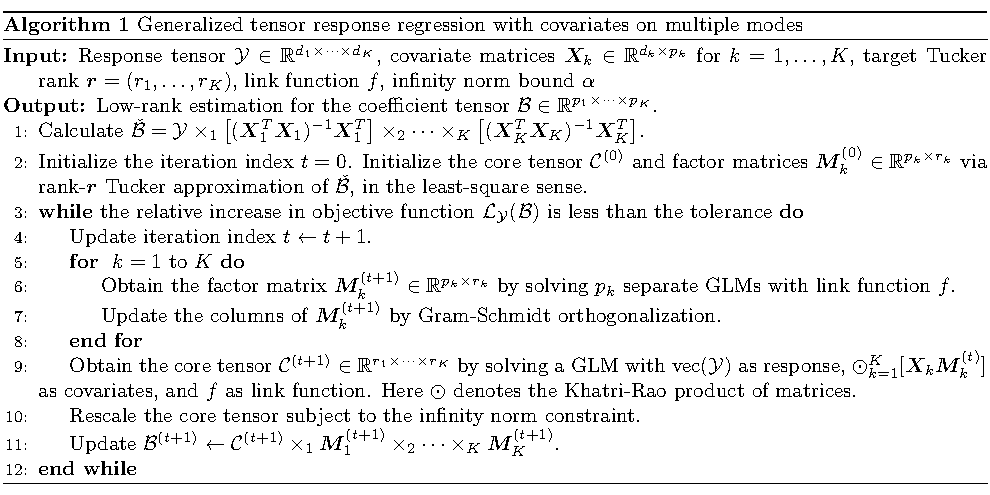
\includegraphics[width=1\textwidth]{algorithm.pdf}
 %DIF <    \label{alg:main}
    %DIF < \caption{\color{red}\fixme{Jiaxin}{Should be $\argmax_{a \in [r] } \cos \of{ \mY_{i:}^d , \mS_{a:}^{(t)}}$. $\sin$ can not handle the obtuse angles; e.g.\ $\sin \pi = \sin 0= 0$, where $\pi$ is not the desired angle.} \fixme{Miaoyan}{Agree. I corrected it.}}
%DIF < \end{figure*}
\DIFaddbegin \DIFadd{We now establish the misclustering error rate of initialization. We call $\mtheta$ is balanced, if the relative extent of heterogeneity is comparable across clusters in that
}\begin{equation}\label{eq:degree}
{\min_{a\in[r]} \onormSize{}{\mtheta_{z^{-1}(a)}}=\left(1+o(1)\right)\max_{a\in[r]}\onormSize{}{\mtheta_{z^{-1}(a)}}}.
\end{equation}
\DIFadd{Note that, the assumption~}\eqref{eq:degree} \DIFadd{does not preclude degree heterogeneity. Indeed, within each of the clusters, the highest degree can be $\theta(i) = \Omega(p)$, whereas the lowest degree can be $\theta(i)=\tO(1)$. 
}\DIFaddend 

\begin{thm}[Error for weighted higher-order initialization]\label{thm:initial} Consider the general \DIFdelbegin %DIFDELCMD < {\color{blue} %%%
\DIFdelend sub-Gaussian \DIFdelbegin %DIFDELCMD < } %%%
\DIFdel{dTBM }%DIFDELCMD < {\color{blue} %%%
\DIFdelend \DIFaddbegin \DIFadd{dTBM }\DIFaddend with i.i.d.\ noise \DIFdelbegin %DIFDELCMD < } %%%
\DIFdelend under the parameter space $\tP$ and Assumption~\ref{assmp:min_gap}. %DIF < With probability at least $1 -C \exp(-cp)$, we have
%DIF < \begin{equation}
%DIF < \min_{\pi \in \Pi}\sum_{i\in[p]}\theta^2_i\ind\{ z^{(0)}(i)\neq \pi \circ z(j)\} \lesssim {Mr^K\sigma^2\over \Delta^2_{\min}}p^{-{(K-2)/2}},
%DIF < \end{equation}
%DIF < where $M>1$ is the relation constant in weighted angle $k$-means. 
Assume $\mtheta$ is balanced and $\min_{i\in[p]}\theta(i) \geq c$ for some constant $c>0$. Let $ z^{(0)}$ denote the output of Sub-algorithm~\hyperref[alg:main]{1}. With probability going to 1, we have
\begin{equation}\label{eq:ini}
   \ell(z^{(0)}, z) \lesssim {r^K p^{-K/2}\over \text{SNR}}. 
\end{equation}
\end{thm}

\begin{rmk}[Comparison to previous results] For fixed SNR, our initialization error rate with $K=2$ agrees with the initialization error rate \DIFdelbegin \DIFdel{$\tO(p)$ }\DIFdelend \DIFaddbegin \DIFadd{$\tO(p^{-1})$ }\DIFaddend in matrix models~\citep{gao2018community}. Furthermore, in the special case of non-degree TBMs \DIFaddbegin \DIFadd{with $\theta_1=\cdots=\theta_p=1$}\DIFaddend , we achieve the same initial misclustering error $\tO(p^{-K/2})$ as in non-degree models~\citep{han2020exact}. Theorem~\ref{thm:initial} implies the advantage of our algorithm in achieving both accuracy and model flexibility. 
%DIF < The result demonstrates the advantage of our algorithm in achieving both accuracy and model flexibility. 
\end{rmk}



%DIF < Assume the number of clusters $r$ is fixed. To ensure the misclassification error $\text{MisClust}(z^{(0)},z)$ decays to 0 as the number of nodes $p \rightarrow \infty$, we need the signal level $\Delta_{\min}^2$ satisfying
%DIF < \begin{equation}
%DIF <     \Delta_{\min}^2/\sigma^2  \gtrsim p^{-K/2}.
%DIF < \end{equation}
%DIF < This implies that desired polynomial rate can be achieved with lower signal level as sample size increases. Moreover, to achieve exact clustering, we should ensure $\text{MisClust}(z^{(0)},z) < \frac{1}{p}$ and thus it requires $\Delta_{\min}^2 \gtrsim p^{2 - K/2}$, which is a fairly strong signal condition especially when $K$ is small. However, the following theorem indicates a weaker signal condition is enough to achieve exact clustering with proper refinement.
\DIFdelbegin %DIFDELCMD < 

%DIFDELCMD < %%%
\DIFdelend \begin{rmk}[Failure of conventional tensor HOSVD] If we use conventional HOSVD for tensor denoising; that is, we use $\mU_{\text{pre}}$ in place of $\hat \mU$ in line 2, then the misclustering rate becomes \DIFdelbegin \DIFdel{$\tO(p)$ }\DIFdelend \DIFaddbegin \DIFadd{$\tO(p^{-1})$ }\DIFaddend for all $K\geq 2$. This rate is substantially worse than our current rate~\eqref{eq:ini}.
\end{rmk}


\DIFdelbegin %DIFDELCMD < {
%DIFDELCMD < \color{blue}
%DIFDELCMD < 

%DIFDELCMD < \begin{rmk}[Eigen free clustering] %%%
\DIFdelend \DIFaddbegin \begin{rmk}[Singular-value gap-free clustering] \DIFaddend Note that our \DIFdelbegin \DIFdel{initialization works on }\DIFdelend \DIFaddbegin \DIFadd{clustering directly applies to }\DIFaddend the estimated mean tensor $\hat \tX$ \DIFdelbegin \DIFdel{directly }\DIFdelend rather than the leading tensor \DIFdelbegin \DIFdel{decomposition factors of $\tX$. On one hand,  clustering on $\hat \tX$ avoids the eigen-gap assumption in previous work~\mbox{%DIFAUXCMD
\cite{ke2019community}}\hspace{0pt}%DIFAUXCMD
. On the other hand,  vanilla spectral methods working on decomposition factors suffers }\DIFdelend \DIFaddbegin \DIFadd{factors $\hat \mU$. Applying clustering to the tensor factors suffers from }\DIFaddend the non-identifiability \DIFdelbegin \DIFdel{of the eigenspace with orthogonal transformation }\DIFdelend \DIFaddbegin \DIFadd{issue due to the infinitely many orthogonal rotations }\DIFaddend when the number of blocks $r \geq 3$ \DIFaddbegin \DIFadd{in the absence of singular-value gaps}\DIFaddend . 
Such ambiguity \DIFdelbegin \DIFdel{comes from the possible multiplicity of eigenvalue and causes }\DIFdelend \DIFaddbegin \DIFadd{causes the }\DIFaddend trouble for effective clustering~\citep{abbe2020entrywise}. In contrast, our \DIFdelbegin \DIFdel{eigen free strategy working on }\DIFdelend \DIFaddbegin \DIFadd{initialization algorithm applies the clustering to the overall mean tensor }\DIFaddend $\hat \tX$\DIFdelbegin \DIFdel{avoids such }\DIFdelend \DIFaddbegin \DIFadd{. This strategy avoids the }\DIFaddend non-identifiability issue regardless \DIFaddbegin \DIFadd{of }\DIFaddend the number of blocks \DIFaddbegin \DIFadd{and singular-value gaps}\DIFaddend .  
\end{rmk}


\DIFdelbegin %DIFDELCMD < }
%DIFDELCMD < 

%DIFDELCMD < %%%
\DIFdelend \subsection{Angle-based iteration}
%DIF < A polynomial-time local iteration refines the initial spectral clustering to achieve an exponential error rate in TBM~\citep{han2020exact}.  
\DIFaddbegin \DIFadd{Our Theorem~\ref{thm:initial} has shown the polynomially decaying error rate from our initialization. Now we improve the error rate to exponential decay using local iterations. }\DIFaddend We propose an angle-based local iteration to improve the outputs from Sub-algorithm~\hyperref[alg:main]{1}. 
To gain the intuition, consider an one-dimensional degree-corrected clustering problem with data vectors $\mx_i = \theta(i) \ms_{z(i)} + \mepsilon_i, i \in [p]$, where $\ms_i$'s are known cluster centroids, $\theta(i)$'s are unknown positive degrees, and $z\colon [p] \mapsto [r]$ is the \DIFdelbegin \DIFdel{clustering }\DIFdelend \DIFaddbegin \DIFadd{cluster }\DIFaddend assignment of interest. The angle-based $k$-means algorithm estimates the assignment $z$ by minimizing the angle between data vectors and centroids; i.e., 
 \begin{equation}\label{eq:angle_kmeans}
     z(i) = \argmax_{a \in [r]} \cos ( \mx_i,\ \ms_{a} ),\ \text{ for all }i \in [p].
 \end{equation}
The classical Euclidean-distance based clustering~\citep{han2020exact} fails to recover $z$ in the presence of degree heterogeneity, even under noiseless case. In contrast, the proposed angle-based $k$-means achieves accurate recovery without explicit estimation of $\mtheta$. 

Our Sub-algorithm~\hyperref[alg:main]{2} shares the same spirit as \DIFaddbegin \DIFadd{in }\DIFaddend angle-based $k$-means. \DIFdelbegin %DIFDELCMD < {\color{blue} %%%
\DIFdelend We still take the order-3 tensor for illustration. \DIFdelbegin %DIFDELCMD < } 
%DIFDELCMD < {
%DIFDELCMD < \color{blue}
%DIFDELCMD < %%%
\DIFdelend Specifically, Sub-algorithm~\hyperref[alg:main]{2} updates estimated core tensor and cluster assignment in each iteration. \DIFaddbegin \DIFadd{We use superscript $\cdot^{(t)}$ to denote the estimate from $t$-th iteration, where $t=1,\ldots.$ }\DIFaddend For core tensor, we consider the following update strategy  
 \[
 \tS^{(t)}(a_1,a_2,a_3)=\text{Ave}\{\tY(i_1,i_2,i_3)\colon z^{(t)}(i_k)=a_k, k\in[3]\}.
\]
Intuitively, $\tS^{(t)}$ becomes closer to the true core $\tS$ as $z^{(t)}$ is more precise. For cluster assignment, we first aggregate the slices of $\tY$ and obtain a reduced tensor $\tY^{\text{d}}\in \bbR^{p \times r \times r}$ with given $z^{(t)}$, where
\[
\tY^{\text{d}}(i,a_2,a_3)=\text{Ave}\{\tY(i,i_2,i_3)\colon z^{(t)}(i_k)=a_k, k \neq 1\}.
\]
\DIFdelbegin \DIFdel{The row $\text{Mat}(\tY^{\text{d}})_{i:}$ and $\text{Mat}(\tS^{(t)})_{a:}$ corresponds }\DIFdelend \DIFaddbegin \DIFadd{We use $\mY^d$ and $ \mS^{(t)}$ to denote the $\text{Mat}(\tY^{\text{d}})$ and $\text{Mat}(\tS^{(t)})$. The rows $\mY^d_{i:}$ and $\mS^{(t)}_{a:}$ correspond }\DIFaddend to the $\mx_i$ and $\ms_a$ \DIFdelbegin \DIFdel{s }\DIFdelend in the one-dimensional clustering~\eqref{eq:angle_kmeans}. Then, we obtain the updated assignment \DIFdelbegin \DIFdel{as
}%DIFDELCMD < \[z(i)^{(t+1)} = \argmin_{a \in [r]} \sin \of{ \mY^{\text{d}}_{i:}, \mS^{(t)}_{a:} }, \text{ for all } i \in [p], \]%%%
\DIFdelend \DIFaddbegin \DIFadd{by
}\[
z(i)^{(t+1)} = \argmax_{a \in [r]} \cos \of{ \mY^{\text{d}}_{i:}, \mS^{(t)}_{a:} },\ \text{ for all } i \in [p],
\]\DIFaddend 
\DIFdelbegin \DIFdel{where $z^{(t+1)}(i)$ is randomly assigned for degenerate rows. }%DIFDELCMD < }
%DIFDELCMD < %%%
%DIF < except that we use estimated centroids $\ms^{(t)}_a$ in place of $\ms_a$ based on estimated assignment in previous iterations. 
\DIFdelend \DIFaddbegin \DIFadd{provided that $\mS^{(t)}_{a:}$ is a non-zero vector. Otherwise, if $\mS^{(t)}_{a:}$ is a zero vector, then we make the convention to assign $z^{(t+1)}(i)$ randomly in $[p]$. }\DIFaddend Full procedures for our angle-based iteration are described in Sub-algorithm~\hyperref[alg:main]{2}. 

We \DIFdelbegin \DIFdel{then }\DIFdelend \DIFaddbegin \DIFadd{now }\DIFaddend establish the misclustering error rate of iterations \DIFdelbegin %DIFDELCMD < { \color{blue} %%%
\DIFdelend under the stability assumption.

\begin{defn}[Locally linear stability] \label{def:stable}
Define the $\varepsilon$-neighborhood of $z$ by $\tN(z,\epsilon)=\{\bar z\colon \ell(\bar z, z)\leq \epsilon\}$. \DIFaddbegin \DIFadd{Let $\bar z\colon[p]\to [r]$ be a clustering function. }\DIFaddend We define two \DIFdelbegin \DIFdel{cluster-size vectors for }\DIFdelend \DIFaddbegin \DIFadd{vectors associated with }\DIFaddend $\bar z$,
\begin{align}
    &\mp(\bar z)=(|\bar z^{-1}(1)|, \ldots,|\bar z^{-1}(r)|)^T, \quad \mp_{\mtheta}(\bar z)=(\onormSize{}{\mtheta_{\bar z^{-1}(1)}}_1,\ldots,\onormSize{}{\mtheta_{\bar z^{-1}(r)}}_1)^T.
\end{align}

We call the degree is $\varepsilon$-locally linearly stable if and only if 
\DIFdelbegin %DIFDELCMD < \begin{equation}
%DIFDELCMD <     \sin(\mp(\bar z),\ \mp_{\mtheta}(\bar z))\lesssim \varepsilon \Delta_{\min} ,\quad \text{for all } \bar z\in \tN(z, \varepsilon).
%DIFDELCMD < \end{equation}%%%
\DIFdelend \DIFaddbegin \begin{equation}\label{eq:local}
    \sin(\mp(\bar z),\ \mp_{\mtheta}(\bar z))\lesssim \varepsilon \Delta_{\min} ,\quad \text{for all } \bar z\in \tN(z, \varepsilon).
\end{equation}\DIFaddend 
\end{defn}
\DIFdelbegin %DIFDELCMD < }
%DIFDELCMD < %%%
\DIFdelend 

\DIFaddbegin \DIFadd{Roughly speaking, the vector $\mp(\bar z)$ represents the raw cluster sizes, and $\mp_{\theta}(\bar z)$ represents the relative cluster sizes weighted by degrees. 
}\DIFaddend The local stability holds trivially for $\varepsilon=0$ based on the construction of parameter space~\eqref{eq:family}. \DIFdelbegin %DIFDELCMD < {\color{blue} %%%
\DIFdel{The locally linear stability avoids the concentration of entities with extremely large or small heterogeneity, when a good estimated assignment with a small misclustering error $\epsilon$ is given.
 }%DIFDELCMD < }
%DIFDELCMD <  %%%
\DIFdelend \DIFaddbegin \DIFadd{The condition~}\eqref{eq:local} \DIFadd{controls the impact of node degree to the $\mp_{\theta}(\cdot)$ with respect to the misclassification rate $\varepsilon$ and angle gap.
 }\DIFaddend 

%DIF <   In Algorithm~\ref{alg:refinement}, the estimated core tensor and cluster assignments are updated in each iteration. For core tensor, notice that the estimator $\tilde S$ with
%DIF <    \[
%DIF <  \tilde \tS(a_1,a_2,a_3)=\text{Ave}\{\tY(i_1,i_2,i_3)\colon z(i_k)=a_k, k\in[3]\}
%DIF <  \]
%DIF <  is an unbiased estimator satisfying $\bbE[\tilde \tS_{a_1,...,a_K}] = \tS_{a_1,...,a_K}$ with true assignment $z$. This leads to a reasonable core tensor update strategy 
%DIF <   \[
%DIF <  \tS^{(t)}(a_1,a_2,a_3)=\text{Ave}\{\tY(i_1,i_2,i_3)\colon z^{(t)}(i_k)=a_k, k\in[3]\}.
%DIF <  \]
%DIF <  Intuitively, the estimate $\tS^{(t)}$ becomes better as $z^{(t)}$ getting more precise. 
\DIFdelbegin %DIFDELCMD < 

%DIFDELCMD < %%%
%DIF <  For cluster assignment, we reduce the higher-order problem to the one-dimensional clustering by matrization. Given $z^{(t)}$, we first aggregate the slices of $\tY$ and obtain a reduced tensor $\tY^{\text{d}}\in \bbR^{p \times r \times r}$, where
%DIF <  \[
%DIF <  \tY^{\text{d}}(i,a_2,a_3)=\text{Ave}\{\tY(i,i_2,i_3)\colon z^{(t)}(i_k)=a_k, k \neq 1\}.
%DIF <  \]
%DIF <  Let $\mY^{\text{d}} = \text{Mat}(\tY^{\text{d}})$ and $\mS^{(t)} = \text{Mat}(\tS^{(t)})$. Then, the row $\mY^{\text{d}}_{i:}$s and $\mS^{(t)}_{a:}$s serve as the data vectors $\mx_i$ and centroids $\ms_a$s in the one-dimensional clustering~\eqref{eq:angle_kmeans}. We obtain the updated assignment as
%DIF <  \begin{equation}
%DIF <      z(i)^{(t+1)} = \argmin_{a \in [r]} \sin \of{ \mY^{\text{d}}_{i:}, \mS^{(t)}_{a:} }, \text{ for all } i \in [p].
%DIF <  \end{equation}
%DIF <  In particular, $z^{(t+1)}(i)$ is randomly assigned for degenerate row with $\onorm{\mY^{\text{d}}_{i:}} = 0$. The refinement outputs the final cluster assignment after $T$ iterations denoted $z^{(T)}$. The full procedure for general order-$K$ tensor is described in Algorithm~\ref{alg:refinement}
%DIFDELCMD < 

%DIFDELCMD < %%%
\DIFdelend \begin{thm}[Error for angle-based iteration]\label{thm:refinement} Consider the setup as in Theorem~\ref{thm:initial}. Assume the local linear stability of degree holds in \DIFdelbegin \DIFdel{all neighborhoods }\DIFdelend \DIFaddbegin \DIFadd{the neighborhood }\DIFaddend $\tN(z,\epsilon)$ for \DIFdelbegin \DIFdel{any $\epsilon \leq \log^{-1}p$}\DIFdelend \DIFaddbegin \DIFadd{$\epsilon \geq \log^{-1}p$}\DIFaddend . Suppose 
$r=\tO(1)$ and $\text{SNR} \gtrsim  p^{-K/2}\log p$. Let $z^{(t)}$ denote the $t$-th iteration output in Sub-algorithm~\hyperref[alg:main]{2} with initialization $z^{(0)}$ from Sub-algorithm~\hyperref[alg:main]{1}. With probability going to 1, there exists a contraction parameter $\rho \in (0,1)$ such that 
\begin{align}\label{eq:final}
    \ell(z, \hat z^{(t+1)}) \lesssim &\ \KeepStyleUnderBrace{
   \text{SNR}^{-1}
    \exp\of{- \frac{p^{K-1}\text{SNR}}{r^{K-1}}}}_{\substack{\text{statistical error}} }+ \KeepStyleUnderBrace{ \rho^t \ell(z, z^{(0)}). }_{\substack{\text{computational error}}}
\end{align}
\end{thm}
\DIFdelbegin \DIFdel{The }\DIFdelend \DIFaddbegin \DIFadd{From the conclusion~}\eqref{eq:final}\DIFadd{, we find that the }\DIFaddend iteration error is decomposed into two parts: statistical error and computational error. The statistical error is unavoidable with noisy data regardless $t$, whereas the computational error decays in an exponential rate as the number of iterations $t \rightarrow \infty$. 

Theorem~\ref{thm:refinement} implies that, with probability going to 1, our estimate $z^{(T)}$ achieves exact recovery within polynomial iterations; more precisely,
\begin{equation}
     z^{(T)} = \pi \circ z, \quad \text{for all }T\gtrsim \log_{1/\rho} p,
\end{equation}
for some permutation $\pi \in \Pi$. \DIFdelbegin %DIFDELCMD < {
%DIFDELCMD < \color{blue} %%%
\DIFdel{We call our algorithm }\DIFdelend \DIFaddbegin \DIFadd{Therefore, our combined algorithm is }\DIFaddend \textit{computationally efficient} \DIFdelbegin \DIFdel{with }\DIFdelend \DIFaddbegin \DIFadd{as long as }\DIFaddend SNR $\gtrsim p^{-K/2} \log p$. Note that\DIFdelbegin \DIFdel{the }\DIFdelend \DIFaddbegin \DIFadd{, ignoring the logarithmic term, the }\DIFaddend minimal SNR requirement, \DIFdelbegin \DIFdel{$p^{-K/2 }\log p$}\DIFdelend \DIFaddbegin \DIFadd{$p^{-K/2}$}\DIFaddend , coincides with the computational lower bound in Theorem~\ref{thm:comp}\DIFdelbegin \DIFdel{ignoring the logarithmic term}\DIFdelend . Therefore, our algorithm is optimal regarding the signal \DIFdelbegin \DIFdel{demand }\DIFdelend \DIFaddbegin \DIFadd{requirement }\DIFaddend and lies in the \DIFdelbegin \DIFdel{most right ``computationally efficient" }\DIFdelend \DIFaddbegin \DIFadd{sharpest }\emph{\DIFadd{computationally efficient}} \DIFaddend regime in Figure~\ref{fig:phase_axis}.
\DIFdelbegin %DIFDELCMD < }
%DIFDELCMD < %%%
\DIFdelend 


\DIFdelbegin %DIFDELCMD < {
%DIFDELCMD < \color{blue}
%DIFDELCMD < %%%
\DIFdelend \subsection{\DIFdelbegin \DIFdel{Extension }\DIFdelend \DIFaddbegin \DIFadd{Extensions }\DIFaddend and practical \DIFdelbegin \DIFdel{issue}\DIFdelend \DIFaddbegin \DIFadd{issues}\DIFaddend }~\label{subsec:exten}
\DIFaddbegin \DIFadd{\hspace{-.3cm} }\DIFaddend {\bf Extension for Bernoulli observations.} The main difficulty to establish the statistical guarantee for Bernoulli observations lies in the initialization \DIFdelbegin \DIFdel{Sub-Algorithm}\DIFdelend \DIFaddbegin \DIFadd{Sub-algorithm}\DIFaddend ~\hyperref[alg:main]{1}. Theorem~\ref{thm:refinement} still holds for Bernoulli observations once the initialization accuracy satisfies the upper bound~\eqref{eq:ini} in Theorem~\ref{thm:initial}.

\DIFdelbegin \DIFdel{Specifically, the }\DIFdelend \DIFaddbegin \DIFadd{We now provide a high-level explanation for the technical difficulty when applying Theorem~\ref{thm:initial} to Bernoulli observations. The }\DIFaddend derivation of Theorem~\ref{thm:initial} relies on the upper bound of the estimation error for the mean tensor in Lemma~\ref{lem:two-step_esterror}\DIFdelbegin \DIFdel{, }\DIFdelend \DIFaddbegin \DIFadd{; }\DIFaddend i.e., with high probability
\begin{equation}\label{eq:prop1}
    \onormSize{}{\hat \tX - \tX}_F^2 \lesssim p^{K/2},
\end{equation}
where \DIFdelbegin \DIFdel{$\tX = \bbE[\tY]$ }\DIFdelend \DIFaddbegin \DIFadd{$\tX = \bbE\tY$ }\DIFaddend and $\hat \tX$ is defined in Step 2 of Sub-algorithm~\hyperref[alg:main]{1}. Unfortunately, the inequality~\eqref{eq:prop1} \DIFdelbegin \DIFdel{only holds }\DIFdelend \DIFaddbegin \DIFadd{holds only }\DIFaddend for i.i.d.\ sub-Gaussian observations while Bernoulli observations are \DIFaddbegin \DIFadd{generally }\DIFaddend not identically distributed.  

One possible remedy is to apply singular value decomposition to the \DIFdelbegin \DIFdel{unfolded Bernoulli observation }\DIFdelend \DIFaddbegin \emph{\DIFadd{square unfolding}}\DIFadd{~\mbox{%DIFAUXCMD
\citep{mu2014square} }\hspace{0pt}%DIFAUXCMD
of Bernoulli tensor }\DIFaddend $\tY$. Let the matrix $\mat_{sq} (\tY) \in \{0,1\}^{\floor{p^{K/2}} \times \ceil{p^{K/2}} }$ denote the \DIFdelbegin \DIFdel{square unfolded binary tensor. We have the estimate 
}%DIFDELCMD < \begin{equation}
%DIFDELCMD <     \hat \tX' = \argmin_{\text{rank}(\mat_{sq}(\tX)) \leq r^{\ceil{K/2}}} \onormSize{}{ \mat_{sq}(\tX)) -  \mat_{sq}(\tY)}_F^2.
%DIFDELCMD < \end{equation}%%%
\DIFdelend \DIFaddbegin \DIFadd{nearly square unfolded Bernoulli tensor. Define a new estimate 
}\begin{equation}\label{eq:matrixsvd}
    \hat \tX' = \argmin_{\text{rank}(\mat_{sq}(\tX)) \leq r^{\ceil{K/2}}} \onormSize{}{ \mat_{sq}(\tX) -  \mat_{sq}(\tY)}_F^2.
\end{equation}\DIFaddend 
\DIFaddbegin \DIFadd{The optimization~}\eqref{eq:matrixsvd} \DIFadd{is simply a matrix SVD problem. }\DIFaddend Following Lemma 7 in \cite{gao2018community}, with high probability, \DIFdelbegin \DIFdel{we have
}\DIFdelend \DIFaddbegin \DIFadd{the new estimate satisfies
}\DIFaddend \begin{equation}
    \onormSize{}{\hat \tX' - \tX}_F^2 \lesssim p^{\ceil{K/2}}.
\end{equation} 
Replacing the estimate $\hat \tX$ by $\hat \tX'$ \DIFaddbegin \DIFadd{in Theorem~\ref{thm:initial}}\DIFaddend , the high probability upper bound for Bernoulli initialization is
\begin{equation}\label{eq:ini_b}
    \ell(z^{(0)}, z) \lesssim \frac{r^K p^{- \floor{K/2} }}{\text{SNR}}. 
\end{equation}
The Bernoulli bound~\eqref{eq:ini_b} is relatively looser than Gaussian bound~\eqref{eq:ini}, especially when $K$ is small. \DIFdelbegin \DIFdel{A tighter Bernoulli bound will be achieved once a low-rank binary tensor estimation scheme with better accuracy is provided in the future }\DIFdelend \DIFaddbegin \DIFadd{Nevertheless, our bound~}\eqref{eq:ini_b} \DIFadd{is already tighter than the pervious work~\mbox{%DIFAUXCMD
\citep{ke2019community}}\hspace{0pt}%DIFAUXCMD
. The investigation of the gap between upper bound $p^{- \floor{K/2}}$ and the lower bound $p^{- K/2}$ for Bernoulli tensors will be left as future work}\DIFaddend . 


{\bf Extension for general dTBMs.} Our two-stage algorithm is able to be extended for the general (asymmetric) dTBMs. Specifically, in the \DIFdelbegin \DIFdel{Sub-Algorithm}\DIFdelend \DIFaddbegin \DIFadd{Sub-algorithm}\DIFaddend ~\hyperref[alg:main]{1}, we make the following changes: (1)
Replace the matrcization $\mat(\tY)$ by $\mat_k(\tY)$; (2) Repeat the Steps 1-5 with mode-specified number of \DIFdelbegin \DIFdel{cluster }\DIFdelend \DIFaddbegin \DIFadd{clusters }\DIFaddend $r_k$; (3) Obtain the collection initialization $ \{z^{(0)}_k\}_{k=1}^K$. In the \DIFdelbegin \DIFdel{Sub-Algorithm}\DIFdelend \DIFaddbegin \DIFadd{Sub-algorithm}\DIFaddend ~\hyperref[alg:main]{2}, we make the following changes: (1) Take the collection $\{z^{(0)}_k\}_{k=1}^K$ as input, and update the block tensor $\tS^{(t)}$ with the collection $\{ z_k^{(t)}\}_{k=1}^K$, $
        \tS^{(t)}(i_1,\ldots, i_K) =  \text{Ave} \{\tY(i_1,\ldots,i_K): z^{(t)}_k(i_k) = j_k, k \in [K]\}$;
(2) Calculate reduced tensor $\tY^{\text{d}}_k$ for each mode via
\begin{align}
    &\tY^{\text{d}}_k(a_1,\ldots,a_{k-1}, i ,a_{k+1},\ldots,a_K) 
    = \text{Ave}\{\tY(i_1,\ldots,i_{k-1},i,i_{k+1},\ldots,i_K): z^{(t)}(i_j) = a_j, j \neq k \}; 
\end{align}

(3) Repeat Step 8-10 with $\mat_k(\cdot), \tY_k^{\text{d}}$ for each $k \in [K]$ and obtain the collection $\{z^{(T)}_k\}_{k=1}^K$. 

Correspondingly, Theorems~\ref{thm:initial} and \ref{thm:refinement} still hold with $\ell(z^{(0)}_k, z_k)$ and $\ell(z^{(t+1)}_k, z_k)$  for all $k \in [K]$. \DIFaddbegin \DIFadd{The detailed model extension for general asymmetric dTBMS can be found in Appendix. 
}\DIFaddend 

{\bf Computational \DIFdelbegin \DIFdel{Complexity}\DIFdelend \DIFaddbegin \DIFadd{complexity}\DIFaddend .} Our two-stage algorithm has a \DIFdelbegin \DIFdel{polynomial computational cost }\DIFdelend \DIFaddbegin \DIFadd{computational cost polynomial in tensor dimension $p$}\DIFaddend . Specifically, the complexity of \DIFdelbegin \DIFdel{Sub-Algorithm}\DIFdelend \DIFaddbegin \DIFadd{Sub-algorithm}\DIFaddend ~\hyperref[alg:main]{1} is $\tO(K p^{K+1} + Krp^K)$, where the first term is contributed by the \DIFdelbegin \DIFdel{first step SVD }\DIFdelend \DIFaddbegin \DIFadd{double projection }\DIFaddend and the calculation of $\hat \tX$, and the second term comes from normalization and the $k$-means. The cost of each update in \DIFdelbegin \DIFdel{Sub-Algorithm}\DIFdelend \DIFaddbegin \DIFadd{Sub-algorithm}\DIFaddend ~\hyperref[alg:main]{2} is $\tO(p^K + pr^K)$, where $p^K$ comes from the calculation of $\tS^{(t)}$ and $\tY^{\text{d}}$\DIFaddbegin \DIFadd{, }\DIFaddend and $pr^K$ comes from the normalization of \DIFdelbegin \DIFdel{$\tY^{\text{d}}, \tS^{(t)}$ }\DIFdelend \DIFaddbegin \DIFadd{$\tY^{\text{d}}$, the calculation of $\tS^{(t)}$, }\DIFaddend and the cluster assignment update in Step 10.

%DIF < that comes from the addition operation and comparison in Step 7,8, and 10. Note that the number of iteration is a logarithmic function of $p$ to achieve exact clustering. We conclude that the two-stage algorithm leads to a polynomial complexity in total.
\DIFdelbegin %DIFDELCMD < 

%DIFDELCMD < %%%
\DIFdelend {\bf \DIFdelbegin \DIFdel{Parameter Selection}\DIFdelend \DIFaddbegin \DIFadd{Hyper-parameter selection}\DIFaddend .} \DIFdelbegin \DIFdel{Note that we assume the }\DIFdelend \DIFaddbegin \DIFadd{In our theoretical analysis, we have assumed the true }\DIFaddend number of clusters $r$ is given \DIFdelbegin \DIFdel{for the algorithm. }\DIFdelend \DIFaddbegin \DIFadd{to our algorithm. In practice, the number of clusters $r$ is often unknown, and we now propose a method to choose $r$ from data. }\DIFaddend We impose the Bayesian information criterion (BIC) and choose the \DIFdelbegin \DIFdel{number of cluster }\DIFdelend \DIFaddbegin \DIFadd{cluster number }\DIFaddend that minimizes BIC\DIFdelbegin \DIFdel{, }\DIFdelend \DIFaddbegin \DIFadd{; }\DIFaddend i.e., under \DIFaddbegin \DIFadd{the symmetric Gaussian }\DIFaddend dTBM~\eqref{eq:model_tensor},
\DIFdelbegin %DIFDELCMD < \begin{equation}
%DIFDELCMD <     \hat r = \argmin_{r \in \mathbb{Z}_+ } \of{ -p^K \tL_{\tY}(\hat z(r), \hat \tS(r), \hat \mtheta(r)) + p_e(r) K \log p},
%DIFDELCMD < \end{equation}%%%
\DIFdelend \DIFaddbegin \begin{align}\label{eq:BIC}
 \hat r &= \argmin_{r \in \mathbb{Z}_+ } \of{p^K \log(\onormSize{}{\hat \tX - \tY}_F^2)  + p_e(r) K \log p},\\
 \text{where}  \quad \hat \tX &= \hat \tS(r) \times_1 \hat \mTheta(r) \hat \mM(r) \times_2 \cdots \times_K \hat \mTheta(r) \hat \mM(r),
\end{align}\DIFaddend 
where the triplet \DIFdelbegin \DIFdel{$(\hat z(r), \hat \tS(r), \hat \mtheta(r))$ }\DIFdelend \DIFaddbegin \DIFadd{$(\hat z(r), \hat \mS(r),\hat \mtheta(r))$ }\DIFaddend are estimated parameters with \DIFdelbegin \DIFdel{given number of cluster }\DIFdelend \DIFaddbegin \DIFadd{cluster number }\DIFaddend $r$, \DIFdelbegin \DIFdel{$\tL_{\tY}$ denote the log-likelihood with observations $\tY$, and $p_e = r^K + p(\log r + 1) - r$ }\DIFdelend \DIFaddbegin \DIFadd{and $p_e (r)= r^K + p(\log r + 1) - r$ }\DIFaddend is the effective number of parameters. \DIFdelbegin \DIFdel{Particularly, we obtain the }\DIFdelend \DIFaddbegin \DIFadd{Note that we have added the argument $(r)$ to related quantities as functions of $r$. In particular, the }\DIFaddend estimate $\hat \mtheta(r)$ \DIFaddbegin \DIFadd{in~}\eqref{eq:BIC} \DIFadd{is obtained }\DIFaddend by first calculating the reduced tensor \DIFdelbegin \DIFdel{$\tY^{\text{d}}$ }\DIFdelend \DIFaddbegin \DIFadd{$\hat \tY^{\text{d}}$ }\DIFaddend with $\hat z(r)$\DIFaddbegin \DIFadd{, }\DIFaddend and then normalizing the row norms \DIFdelbegin \DIFdel{$\onormSize{}{\mY_{i:}^{\text{d}}}$ }\DIFdelend \DIFaddbegin \DIFadd{$\onormSize{}{\hat \mY_{i:}^{\text{d}}}$ }\DIFaddend to 1 in each cluster; i.e., 
\DIFdelbegin %DIFDELCMD < \begin{equation}
%DIFDELCMD <     \hat \theta(i,r) = \frac{\onormSize{}{\hat \mY^{\text{d}}(r)_{i:}}}{\sum_{j: \hat z(j,r) =  \hat z(i,r)} \onormSize{}{\hat \mY^{\text{d}}(r)_{j:}}},
%DIFDELCMD < \end{equation}%%%
\DIFdelend \DIFaddbegin \begin{equation}
 \hat \mtheta(r)=(\hat \theta(1,r),\ldots,\hat \theta(p,r))^T,\quad\text{where}\quad   \hat \theta(i,r) = \frac{\onormSize{}{\hat \mY^{\text{d}}(r)_{i:}}}{\sum_{j: \hat z(j,r) =  \hat z(i,r)} \onormSize{}{\hat \mY^{\text{d}}(r)_{j:}}},
\end{equation}\DIFaddend 
where $\hat \mY^{\text{d}}(r) = \mat(\hat \tY^{\text{d}}(r))$\DIFdelbegin \DIFdel{and 
}%DIFDELCMD < \begin{equation}
%DIFDELCMD <     \hat \tY^{\text{d}}(r)(i,a_2,\ldots,a_K) = 
%DIFDELCMD < \text{Ave}\{\tY(i,i_2,\ldots,i_K): \hat z(i_k, r) = a_k, k \neq 1 \}.
%DIFDELCMD < \end{equation}
%DIFDELCMD < 

%DIFDELCMD < %%%
\DIFdel{With Gaussian observation $\tY$, we have
}%DIFDELCMD < \begin{equation}
%DIFDELCMD <     \tL_{\tY} = - \log(\onormSize{}{\hat \tX - \tY}_F^2), \quad \hat \tX = \tS(r) \times_1 \hat \mTheta(r) \hat \mM(r) \times_2 \cdots \times_K \hat \mTheta(r) \hat \mM(r).
%DIFDELCMD < \end{equation}
%DIFDELCMD < %%%
\DIFdelend \DIFaddbegin \DIFadd{, $\hat \tY^{\text{d}}(r)(i,a_2,\ldots,a_K) =  \text{Ave}\{\tY(i,i_2,\ldots,i_K): \hat z(i_k, r) = a_k, k \neq 1 \}$, and $\hat z(i,r)$ denotes the community label for the $i$-th node with given cluster number $r$. }\DIFaddend We evaluate the performance of the BIC criterion in Section~\ref{subsec:num_theory}.


%DIF <  We here provide a simple rank selection criteria when $r$ is unknown. With a fixed $r$, calculate the estimated minimal gap
%DIF <  \begin{equation}
%DIF <      \hat \Delta_{\min}(r) = \min_{a \neq b \in [r]} \onorm{ \frac{\hat \mS_{a:}(r)}{\onormSize{}{\hat \mS_{a:}(r)}} - \frac{\hat \mS_{b:}(r)}{\onormSize{}{\hat \mS_{b:}(r)}} },
%DIF <  \end{equation}
%DIF <  where $\mS(r) = \mat(\hat \tS(r))$ and $\hat \tS(r)$ is the estimated signal tensor obtained by the same procedure in Step 7 of Sub-Algorithm~\hyperref[alg:main]{2} with the estimated assignment $\hat z(r)$. With a given upper bound for the number of clusters, denoted $R$, we choose $r$ that maximizes the estimated minimal gap, i.e.,
%DIF <  \begin{equation}
%DIF <      \hat r = \argmax_{r \in [R]} \hat \Delta_{\min}(r).
%DIF <  \end{equation}
\DIFdelbegin %DIFDELCMD < 

%DIFDELCMD < }
%DIFDELCMD < 

%DIFDELCMD < %%%
%DIF < We now discuss the conditions for which exact recovery occurs, i.e., $\ell(z, \hat z^{(t+1)})=0$ for some $t\geq T=\text{poly}(p)$. Based on Theorem~\ref{thm:refinement}, we need
%DIF < \[
%DIF < T\geq \log p +\log \ell(z, \hat z^{(0)})
%DIF < \]
%DIF < given initial assignment $z^{(0)}$ from Algorithm~\ref{alg:initial} and iteration number $T \geq 2 \log p$, with probability going to 1, the output of our Algorithm~\ref{alg:refinement} achieves exact recovery, i.e., for some permutation $\pi \in \Pi$,
%DIF < \begin{equation}
 %DIF <     z^{(T)} = \pi \circ z, \quad \text{for all }T\geq 2\log p.
%DIF < \end{equation}
%DIFDELCMD < 

%DIFDELCMD < %%%
%DIF < \begin{algorithm}[h]
%DIFDELCMD < 

%DIFDELCMD < %%%
%DIF < \caption{Angle-based iteration}\label{alg:refinement}
%DIF < \begin{algorithmic}[1]
%DIFDELCMD < 

%DIFDELCMD < %%%
%DIF < \INPUT Observation $\tY \in \bbR^{p \times \cdots \times p}$, initialization $z^{(0)} \colon [p]\to[r]$, iteration number $T$.
%DIF < \For {$t = 0$ to $T-1$}
%DIF < \State Update the block tensor $\tS^{(t)}$ via
%DIF < \begin{align}
%DIF <     &\tS^{(t)} (i_1,...,i_K)\\
 %DIF <    & \quad = \text{Ave} \{\tY(i_1,\ldots,i_K): z^{(t)}(i_k) = j_k, k \in [K]\}
%DIF < \end{align}
%DIF < \State Calculate reduced tensor $\tY^{\text{d}} \in \bbR^{p \times r \times \cdots \times r}$
%DIF < \begin{align}
%DIF <     &\tY^{\text{d}}(i,a_2,\ldots,a_%K) \\
%DIF <     &= 
%DIF < \text{Ave}\{\tY(i,i_2,\ldots,i_K): z^{(t)}(i_k) = a_k, k \neq 1 \}
%DIF < \end{align}
%DIFDELCMD < 

%DIFDELCMD < %%%
%DIF < \State Let $\mY^{\text{d}} = \text{Mat}(\tY^{\text{d}})$ and $J_0 = \{ i\in[p]: \onorm{\mY^{\text{d}}_{i:}} = 0\}$. Set $z^{(t+1)}(i)$ randomly in $[r]$ for $i \in J_0$.
%DIFDELCMD < 

%DIFDELCMD < %%%
%DIF < \State Let $\mS^{(t)} = \text{Mat}(\tS^{(t)})$. For all $i \in J_0^c$ update cluster assignment by
%DIF < \begin{equation}
%DIF <     z(i)^{(t+1)} = \argmin_{a \in [r]} \sin \of{ \mY^{\text{d}}_{i:}, \mS^{(t)}_{a:} }.
%DIF < \end{equation}
%DIFDELCMD < 

%DIFDELCMD < %%%
%DIF < \EndFor
%DIFDELCMD < 

%DIFDELCMD < %%%
%DIF < \OUTPUT Estimated clustering $z^{(T)}  \in [r]^{p}$.
%DIF < \end{algorithmic}
%DIF < \end{algorithm}
%DIFDELCMD < 

%DIFDELCMD < %%%
%DIF < We refer to the combination of Algorithms~\ref{alg:initial}+ \ref{alg:refinement} as provable dTBM algorithm. 
%DIFDELCMD < 

%DIFDELCMD < %%%
%DIF < \fixme{Miaoyan}{add discussion as in my JMLR binary tensor paper (stat-comp dominating terms)}
%DIFDELCMD < 

%DIFDELCMD < %%%
\DIFdelend \section{Numerical studies}\label{sec:simulation}

 We evaluate the performance of the weighted higher-order initialization and angle-based iteration in this section. We report average errors and standard deviations across 30 replications in each experiment. Clustering accuracy is assessed by clustering error rate (CER, i.e., one minus rand index). Note that CER between $(\hat z, z)$ is equivalent to misclustering error $\ell(\hat z, z)$ up to constant multiplications~\citep{meilua2012local}, and a lower CER indicates a better performance.

We generate order-3 tensors with \emph{assortative}~\citep{gao2018community} core tensors to control SNR; i.e., we set $\tS_{aaa} = s_1$ for $a \in [r]$ and others be $s_2$, where $s_1 > s_2 > 0$. Let $\alpha = s_1/s_2$. We set $\alpha$ close to 1 such that $1-\alpha=o(p)$. In particular, we have $\alpha = 1 + \Omega(p^{\gamma/2})$ %DIF < \fixme{Miaoyan}{My calculation shows $\text{SNR}=\Omega((1-\alpha)^2)\Rightarrow \alpha=1+\Omega(p^{\gamma/2})$. Double check.} 
  \DIFaddbegin \DIFadd{with $\gamma<0$ }\DIFaddend by Assumption~\ref{assmp:min_gap} and definition~\eqref{eq:gamma}. Hence, we easily adjust SNR via varying $\alpha$. %DIF < We also set $\onorm{\text{Mat}(\tS)_{a:}} = c$ for some $c>0$ to exclude the effect of signal magnitude. 
 Note that the assortative setting is proposed for simulations, and our algorithm is applicable for general tensors in practice. The cluster assignment $z$ is randomly generated with equal probability across  $r$ clusters for each mode. Without further explanation, we generate degree heterogeneity $\mtheta$ from absolute normal distribution \DIFdelbegin \DIFdel{as }\DIFdelend \DIFaddbegin \DIFadd{by }\DIFaddend $\theta(i) = |X_i| + 1 - 1/\sqrt{2\pi}$ with $|X_i| \stackrel{\text{i.i.d.}}\sim N(0,1), i \in [p]$ and normalize $\mtheta$ to satisfy \eqref{eq:family}. Also, we set $\sigma^2 = 1$ for Gaussian data without further specification. 

%DIF <   To control SNR, we generate ``assortative" core tensors for all experiments, as a higher-order analogy of the setting in \citep{gao2018community}; i.e.,
%DIF <  \begin{align} \tS_{ijk} = 
%DIF <      \begin{cases}
%DIF <      s_1 & \text{if } i = j = k,\\
%DIF <      s_2 & \text{if $i,j,k$ are not identical, }
%DIF <      \end{cases}
%DIF <  \end{align}
%DIF <  where $s_1 > s_2 > 0$. Let $\alpha = s_1/s_2$ be the ratio between diagonal and off-diagonal elements. We have $\alpha = 1 + \Omega(p^{\gamma})$ by Assumption~\ref{assmp:min_gap} and definition~\eqref{eq:gamma} with fixed $\sigma^2$. This helps us to easily adjust SNR via varying $\alpha$. We also set $\onorm{\text{Mat}(\tS)_{a:}} = c$ for some $c>0$ to exclude the effect of signal magnitude. The ``assortative" setting is proposed for convenience. In practice, our algorithm is applicable for general core tensor. 
\DIFdelbegin %DIFDELCMD < 

%DIFDELCMD < %%%
%DIF <  The cluster assignment $z$ is randomly generated with given integer $r$. Without specific explanation, we generate degree heterogeneity $\mtheta$ from absolute normal distribution as $\theta(i) = |X_i| + 1 - 1/\sqrt{2\pi}, i \in [p]$ with $|X_i| \sim_{i.i.d.} N(0,1)$ and normalize $\mtheta$ to satisfy \eqref{eq:family}. We generate the noisy tensor under Gaussian model with $\sigma^2 = 1$ and Bernoulli model with mean tensor  $\tS \times_1 \mTheta \mM \times_2 \mTheta \mM \times_3 \mTheta \mM$. We denote provable dTBM algorithm as \textbf{Ours} for simplicity.
%DIFDELCMD < 

%DIFDELCMD < %%%
\DIFdelend \subsection{Verification of theoretical results}\label{subsec:num_theory}

The first experiment verifies  statistical-computational gap described in Section~\ref{sec:limits}. Consider the Gaussian model with $p = \{80, 100\}$, $r = 5$. We vary $\gamma $ in $ [-1.2, -0.4]$ and $[-2.1, -1.4]$ for matrix ($K=2$) and tensor $(K = 3)$ clustering, respectively. Note that finding MLE under dTBM is computationally intractable. We approximate MLE using an oracle estimator\DIFdelbegin \DIFdel{; }\DIFdelend \DIFaddbegin \DIFadd{, }\DIFaddend i.e., the output of Sub-algorithm~\hyperref[alg:main]{2} initialized from true assignment. Figure~\ref{fig:phase}a shows that both our algorithm and oracle estimator start to decrease around the critical value $\gamma_{\text{stat}}  = \gamma_{\text{comp}}  = -1$ in matrix case. In contrast, Figure~\ref{fig:phase}b shows a significant gap in the phase transitions between the algorithm estimator and oracle estimator in tensor case. The oracle error rapidly decreases to 0 when $\gamma_{\text{stat}} = -2$, whereas the algorithm estimator tends to achieve exact clustering when $\gamma_{\text{comp}} = -1.5$. Figure~\ref{fig:phase} confirms the existence of the statistical-computational gap in our Theorems~\ref{thm:stats} and~\ref{thm:comp}. 


%DIF < \fixme{Miaoyan}{\color{red} add spacing between two figure panels}
\begin{figure}[htb]
    \centering
    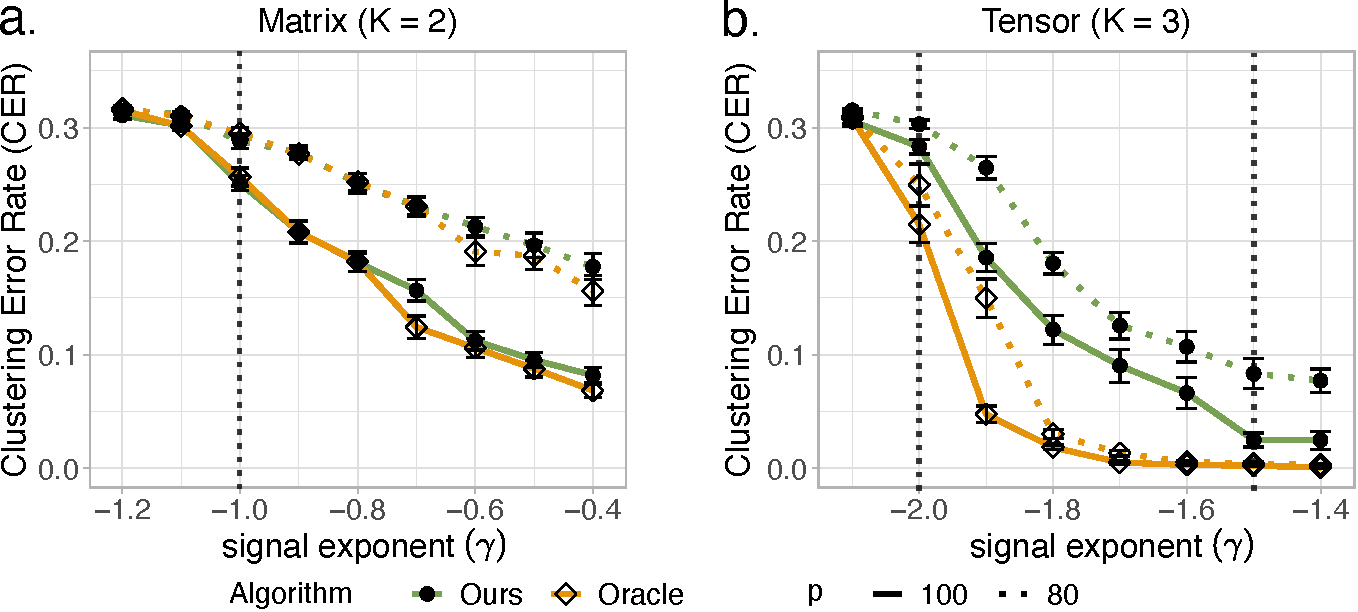
\includegraphics[width=.8\columnwidth]{phase_anno3.pdf}
    \caption{SNR phase transitions for clustering in dTBM with $p = \{80, 100\}, r = 5$ under (a) matrix case with $\gamma \in [-1.2, -0.4]$ and (b) tensor case with $ \gamma \in [-2.1, -1.4]$.
    }
    \label{fig:phase}
\end{figure}

The second experiment verifies the performance guarantees of two algorithms: (i) weighted higher-order initialization; (ii) combined algorithm of weighted higher-order initialization and angle-based iteration. We consider both the Gaussian and Bernoulli models with $p = \{80, 100\}$, $r = 5$, $\gamma \in [-2.1, -1.4]$. %DIF < We set $c = 0.5$ and $c = 0.25$ for Gaussian and Bernoulli cases, respectively. 
Figure~\ref{fig:ini_re} shows the substantial improvement of combined algorithm over initialization, especially under weak and intermediate signals. This phenomenon agrees with the error rates in Theorems~\ref{thm:initial} and \ref{thm:refinement} 
and confirms the necessity of the local iterations.

\begin{figure}[htp!]
    \centering
     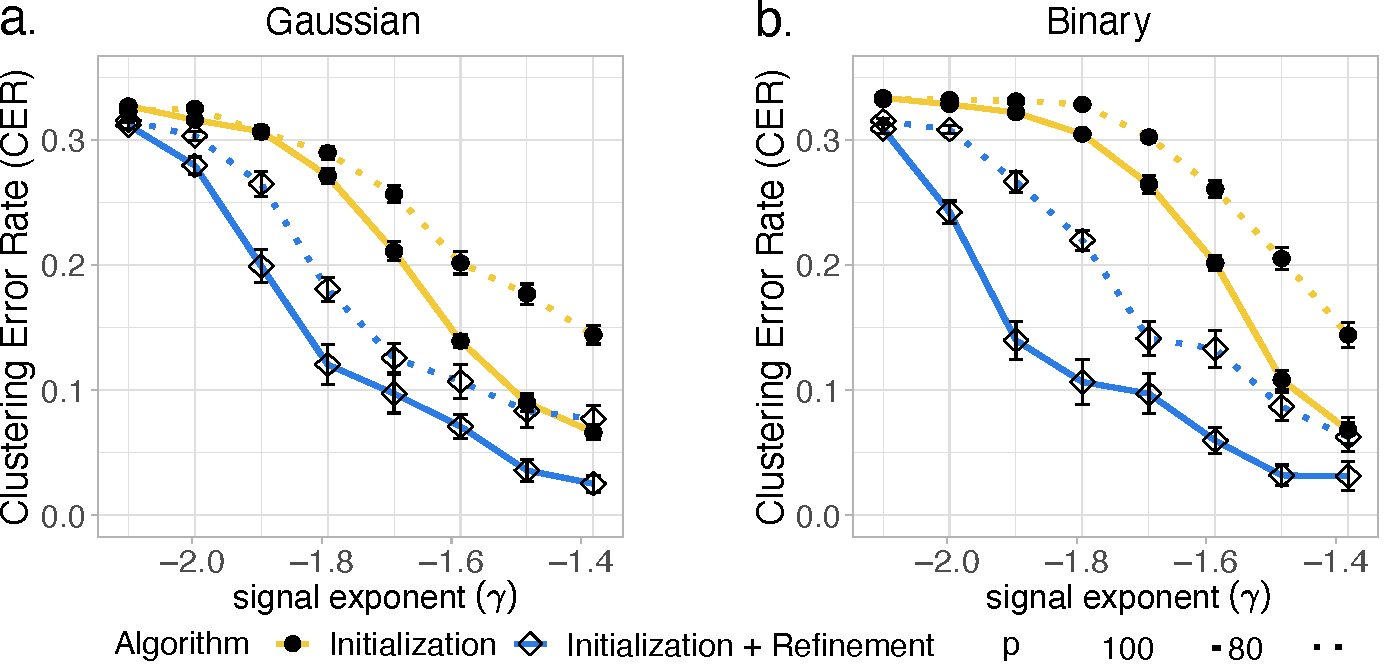
\includegraphics[width=.8\columnwidth]{ini_re_anno3.pdf}
    \caption{CER versus signal exponent $(\gamma)$ for initialization only and for combined algorithm. We set $p = \{80, 100\}, r = 5, \gamma \in [-2.1, -1.4]$ under (a) Gaussian models and (b) Bernoulli models. }
    \label{fig:ini_re}

\end{figure}


\DIFdelbegin %DIFDELCMD < {
%DIFDELCMD < \color{blue} 
%DIFDELCMD < 

%DIFDELCMD < %%%
%DIF <  \begin{table}[hbt]
%DIF <  \color{blue}
%DIF <      \centering
    %DIFDELCMD < 

%DIFDELCMD < %%%
%DIF <      \begin{tabularx}{\textwidth}{c *{12}{Y}}
%DIF <      \toprule
%DIF <      Settings & \multicolumn{3}{c}{$p = 50, \sigma^2 = 0.25$} & \multicolumn{3}{c}{$p = 50, \sigma^2 = 1$} & \multicolumn{3}{c}{$p = 80, \sigma^2 = 0.25$} & \multicolumn{3}{c}{$p = 80, \sigma^2 = 1$}\\
%DIF <      \cmidrule(lr){2-4} \cmidrule(l){5-7} \cmidrule(l){8-10} \cmidrule(l){11-13}
%DIF <           True number of clusters $r$ & 2&3 & 4 & 2 & 3 & 4 & 2 & 3 & 4 & 2 & 3 & 4  \\
%DIF <           \midrule
%DIF <           Estimated number of clusters $\hat r$ &  2 & 3 & 3.9(0.3)& 2 & 3  & 3.1(0.5) & 2  & 3  & 4  & 2  & 3 & 3.9(0.31)   \\
%DIF <       \bottomrule
%DIF <      \end{tabularx}
%DIF <      \caption{Estimated number of clusters given by BIC criterion under the small noise $(\sigma^2 = 0.25)$ and large noise $(\sigma^2 = 0.5)$ cases. Numbers in parentheses are standard deviations of $\hat r$ over 30 replications.}
%DIF <      \label{tab:select}
%DIF <  \end{table}
%DIFDELCMD < 

%DIFDELCMD < %%%
\DIFdelend \begin{table}[hbt]
\DIFdelbeginFL %DIFDELCMD < \color{blue}
%DIFDELCMD <     %%%
\DIFdelendFL \centering
    \DIFdelbeginFL %DIFDELCMD < 

%DIFDELCMD <     %%%
\DIFdelendFL \begin{tabularx}{\textwidth}{c *{8}{Y}}
    \toprule
    Settings & \multicolumn{2}{c}{$p = 50, \sigma^2 = 0.25$} & \multicolumn{2}{c}{$p = 50, \sigma^2 = 1$} & \multicolumn{2}{c}{$p = 80, \sigma^2 = 0.25$} & \multicolumn{2}{c}{$p = 80, \sigma^2 = 1$}\\
    \cmidrule(lr){2-3} \cmidrule(l){4-5} \cmidrule(l){6-7} \cmidrule(l){8-9}
         True number of clusters $r$ & 2 & 4 & 2  & 4 & 2  & 4 & 2 & 4  \\
         \midrule
         Estimated number of clusters $\hat r$ &  2(0)  & 3.9(0.25)& 2(0)    & 3.1(0.52) & 2(0)    & 4(0)   & 2(0)    & 3.9(0.31)   \\
     \bottomrule
    \end{tabularx}
    \caption{Estimated number of clusters given by BIC criterion under the \DIFdelbeginFL \DIFdelFL{small }\DIFdelendFL \DIFaddbeginFL \DIFaddFL{low }\DIFaddendFL noise $(\sigma^2 = 0.25)$ and \DIFdelbeginFL \DIFdelFL{large }\DIFdelendFL \DIFaddbeginFL \DIFaddFL{high }\DIFaddendFL noise $(\sigma^2 = 0.5)$ \DIFdelbeginFL \DIFdelFL{cases}\DIFdelendFL \DIFaddbeginFL \DIFaddFL{settings}\DIFaddendFL . Numbers in parentheses are standard deviations of $\hat r$ over 30 replications.}
    \label{tab:select}
\end{table}

The third experiment evaluates the empirical performance of the BIC criterion to select unknown number of \DIFdelbegin \DIFdel{cluster}\DIFdelend \DIFaddbegin \DIFadd{clusters}\DIFaddend . We generate the data from an order-3 Gaussian model with $p = \{50,80\}$, $r = \{2,4\}$\DIFdelbegin \DIFdel{and consider the noise }\DIFdelend \DIFaddbegin \DIFadd{, and noise level }\DIFaddend $\sigma^2 \in \{ 0.25,1\}$\DIFdelbegin \DIFdel{with $\alpha = 400$}\DIFdelend . Table~\ref{tab:select} \DIFdelbegin \DIFdel{implies }\DIFdelend \DIFaddbegin \DIFadd{shows }\DIFaddend that our BIC criterion \DIFdelbegin \DIFdel{exactly choose }\DIFdelend \DIFaddbegin \DIFadd{well chooses }\DIFaddend the true $r$ under \DIFdelbegin \DIFdel{all the settingswith small $r = 2$}\DIFdelend \DIFaddbegin \DIFadd{most settings}\DIFaddend .  Note that the BIC \DIFdelbegin \DIFdel{underestimates the large }\DIFdelend \DIFaddbegin \DIFadd{slightly underestimates the }\DIFaddend true number of clusters $(r = 4)$ with smaller \DIFdelbegin \DIFdel{SNR $(\sigma^2 = 1)$}\DIFdelend \DIFaddbegin \DIFadd{dimension and higher noise $(p = 50, \sigma=1)$}\DIFaddend , and the accuracy immediately increases with larger dimension $p = 80$. The improvement follows \DIFdelbegin \DIFdel{by }\DIFdelend \DIFaddbegin \DIFadd{from }\DIFaddend the fact that a larger dimension $p$ indicates a larger sample size in the \DIFaddbegin \DIFadd{tensor }\DIFaddend block model. Therefore, we conclude that BIC criterion is a reasonable way to tune the number of clusters.
\DIFdelbegin %DIFDELCMD < }
%DIFDELCMD < %%%
%DIF <  {
%DIF <  \color{red} 
%DIF <  More experiments:
%DIF <  \begin{enumerate}
%DIF <      \item Initialization impact to Angle-based iteration.(Figure 4 in Han)
%DIF <      \item Imbalanced cluster size.(Figure 9 in Han)
%DIF <      \item Non-degree comparison. 
%DIF <  \end{enumerate}
%DIF <  }
\DIFdelend 


\subsection{Comparison with other methods}\label{subsec:comp}


We compare our algorithm with following higher-order clustering methods:
\begin{itemize}[wide,topsep=-3pt,itemsep=0pt,parsep=1pt]
    \item \textbf{\small HOSVD}: HOSVD on data tensor and $k$-means on the rows of the factor matrix;
    \item \textbf{\small HOSVD+}: HOSVD on data tensor and $k$-means on the $\ell_2$-normalized rows of the factor matrix;
    \item \textbf{\small HLloyd}\DIFaddbegin \DIFadd{~\mbox{%DIFAUXCMD
\citep{han2020exact}}\hspace{0pt}%DIFAUXCMD
}\DIFaddend : High-order \DIFdelbegin \DIFdel{Lloyd algorithm and high-order spectral clustering ~\mbox{%DIFAUXCMD
\citep{han2020exact}}\hspace{0pt}%DIFAUXCMD
}\DIFdelend \DIFaddbegin \DIFadd{clustering algorithm developed for non-degree tensor block models}\DIFaddend ;
    \item \textbf{\small SCORE}\DIFaddbegin \DIFadd{~\mbox{%DIFAUXCMD
\citep{ke2019community}}\hspace{0pt}%DIFAUXCMD
}\DIFaddend : Tensor-SCORE for clustering \DIFdelbegin \DIFdel{~\mbox{%DIFAUXCMD
\citep{ke2019community}}\hspace{0pt}%DIFAUXCMD
;
    %DIF < \item \textbf{\small SCORE-}: Incomplete tensor-SCORE without regularized higher-order orthogonal iteration.
}\DIFdelend \DIFaddbegin \DIFadd{developed for binary tensors.
}\DIFaddend \end{itemize}


Among the four alternative algorithms, the \textbf{\small SCORE} is the closest method to ours. %DIF < , since \textbf{\small SCORE} also The incomplete version \textbf{\small SCORE-} skips the key step, regularized HOOI, in \textbf{\small SCORE}. We involve \textbf{\small SCORE-} to study the critical components of \textbf{\small SCORE}. 
We set the tuning parameters of \textbf{\small SCORE} as in previous literature \citep{ke2019community}. The methods \textbf{\small SCORE} and \textbf{\small HOSVD+} are designed for degree models, whereas \textbf{\small HOSVD} and \textbf{\small HLloyd} are designed for non-degree models. %DIF < which shares a similar idea of our spectral initialization but implements naive denoising and clustering steps.  We refer our algorithm as \textbf{\small dTBM}.
%DIF < , and the later one is expected to outperform than spectral methods under TBM. 
We conduct two experiments to assess the impacts of (i) signal strength and (ii) degree heterogeneity, based on Gaussian and Bernoulli models with $ p = 100, r = 5$. We refer to our algorithm as \textbf{\small dTBM} in the comparison. 
%DIF < Consider $ p = 100, r = 5, c = 0.5$ for both experiments. 

We investigate the effects of signal to clustering performance by varying $\gamma \in [-1.5, -1.1]$. Figure~\ref{fig:comp_gamma} shows the consistent outperformance of our method \textbf{\small dTBM} among all algorithms. The sub-optimality of \textbf{\small SCORE} and \textbf{\small HOSVD+} indicates the necessity of local iterations on the clustering. Furthermore,  Figure~\ref{fig:comp_gamma} shows the inadequacy of non-degree algorithms in the presence of mild degree heterogeneity. 
The experiment demonstrates the benefits of addressing heterogeneity in higher-order clustering tasks.   


\begin{figure}[h!]
    \centering
    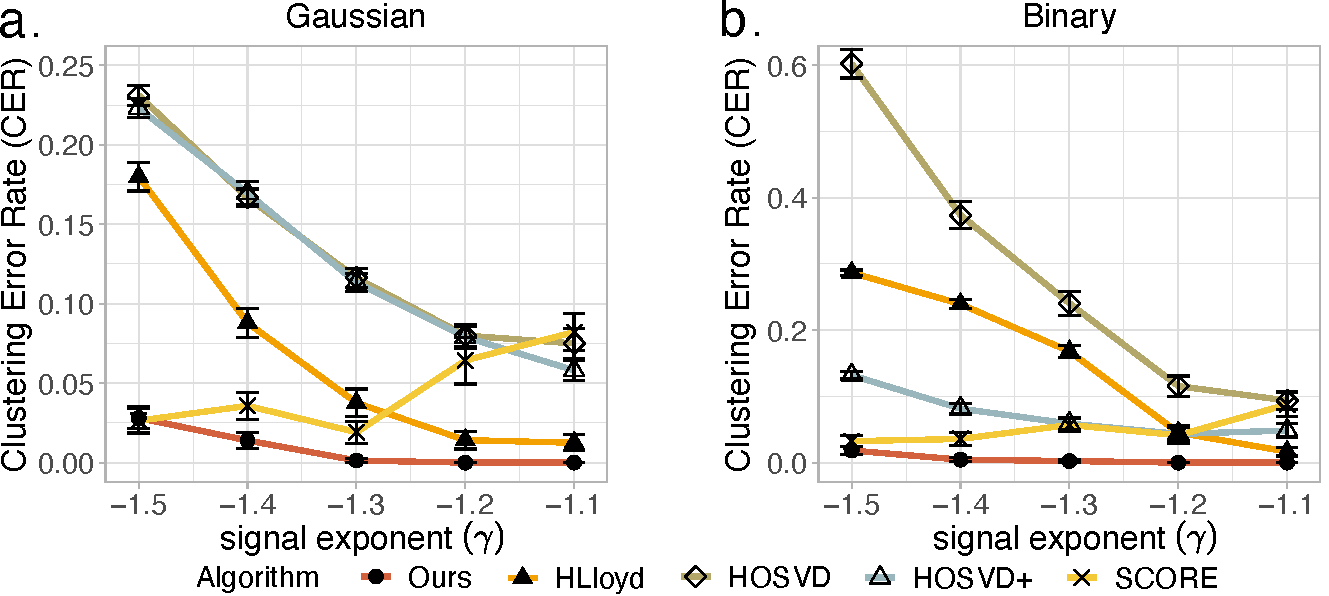
\includegraphics[width=.8\columnwidth]{comp_gamma_anno3.pdf}
    \caption{CER versus signal exponent (denoted $\gamma$) for different methods. We set $p = 100, r = 5, \gamma \in [-1.5, -1.1]$ under (a) Gaussian and (b) Bernoulli models.}
    \label{fig:comp_gamma}
\end{figure}


The only exception in Figure~\ref{fig:comp_gamma} is the slightly better performance of \textbf{\small HLloyd} over \textbf{\small HOSVD+} under Gaussian model. However, we find the advantage of \textbf{\small HLloyd} disappears with higher degree heterogeneity. We perform extra simulations to verify the impact of degree effects. We use the same setting as in the first experiment in the Section~\ref{subsec:comp}, except that we now generate the degree heterogeneity $\mtheta$ from Pareto distribution \DIFdelbegin \DIFdel{with shape parameter $a$ }\DIFdelend prior to normalization. \DIFdelbegin \DIFdel{We }\DIFdelend \DIFaddbegin \DIFadd{The density function of Pareto distribution is $f(x|a,b) = a b^a x^{-(a+1)} \ind\{ x \geq b \}$, where $a$ is called }\emph{\DIFadd{shape}} \DIFadd{parameter. We vary $a \in \{2,6\}$ and choose $b$ such that $\bbE X = a(a - 1)^{-1}b = 1$ for $X$ following Pareto$(a,b)$. Note that a smaller $a$ leads to a larger variance in $\mtheta$ and hence a larger degree heterogeneity. We }\DIFaddend consider the Gaussian model under low $(a = 6)$ and high $(a = 2)$ degree heterogeneity. Figure~\ref{fig:comp_gamma_theta} shows that the errors for non-degree algorithms (\textbf{\small HLloyd}, \textbf{\small HOSVD}) \DIFdelbegin \DIFdel{increases }\DIFdelend \DIFaddbegin \DIFadd{increase }\DIFaddend with degree heterogeneity. In addition, the advantage of \textbf{\small HLloyd} over \textbf{\small HOSVD+} disappears with higher degree heterogeneity. 



%DIF < Figure~\ref{fig:comp_gamma} implies all methods perform better with larger signal. Our \textbf{\small dTBM} and \textbf{\small SCORE} show the best accuracy as expected. The sub-optimality of \textbf{\small SCORE-} and \textbf{\small HOSVD ++} implies the necessity of local refinement for spectral clustering. A surprising observation is that \textbf{\small HLloyd} beats  \textbf{\small SCORE-} and \textbf{\small HOSVD ++} under Gaussian case, which indicates the robustness of \textbf{\small HLloyd} for mild heterogeneity.
\DIFdelbegin %DIFDELCMD < 

%DIFDELCMD < %%%
\DIFdelend \begin{figure}[h!]
    \centering
    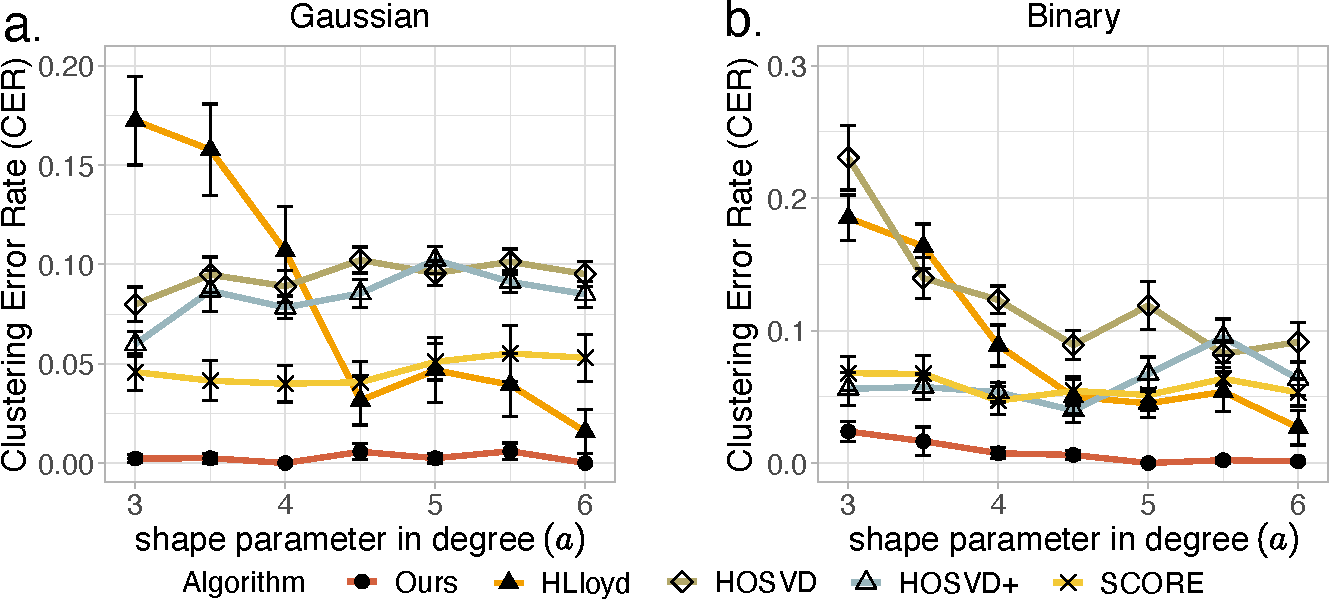
\includegraphics[width=.8\columnwidth]{comp_theta_anno3.pdf}
    \caption{CER versus shape parameter in degree (denoted $a\in[3,6]$) for different methods. We set $p = 100, r = 5, \gamma = -1.2$ under (a) Gaussian and (b) Bernoulli models.}
    \label{fig:comp_theta}
\end{figure}



\begin{figure}[htp!]
    \centering
    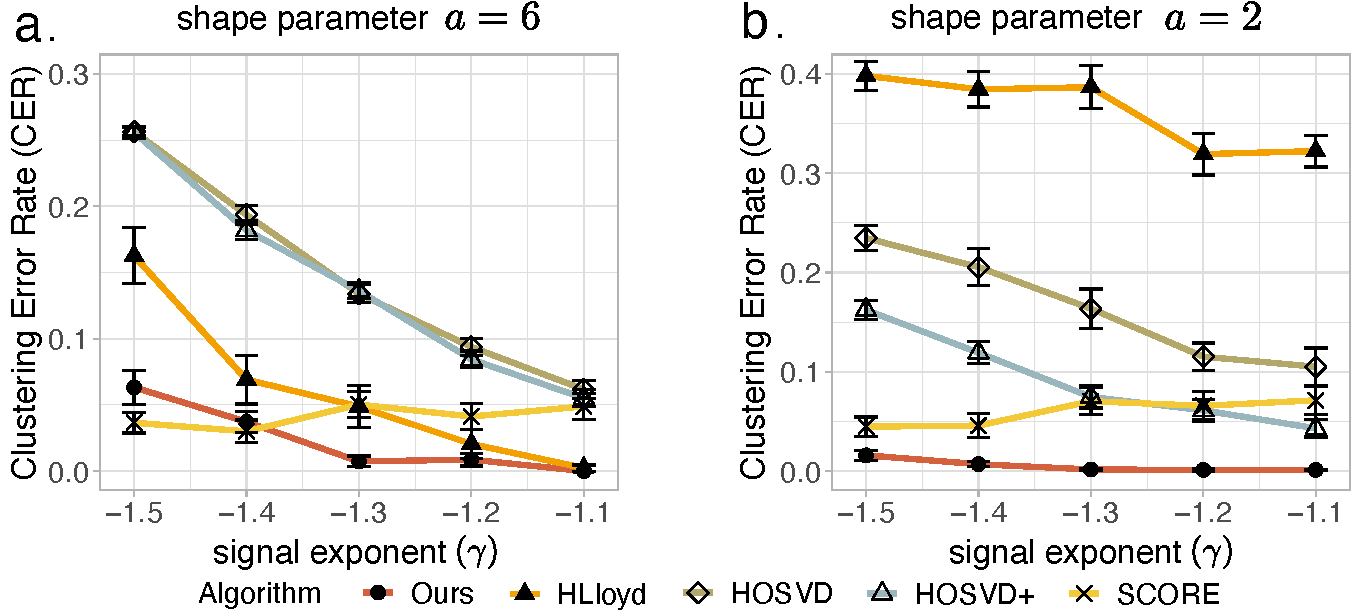
\includegraphics[width=.8\columnwidth]{comp_gamma_theta3.pdf}
    \caption{CER comparison versus signal exponent (denoted $\gamma$) under (a) low (shape parameter $a = 6$)  (b) high (shape parameter $a = 2$) degree heterogeneity. We set $p = 100, r = 5, \gamma \in [-1.5, -1.1]$ under Gaussian model.}
    \label{fig:comp_gamma_theta}
\end{figure}

The last experiment investigates the effects of degree heterogeneity to clustering performance. We fix the signal exponent $\gamma = -1.2$ and vary the extent of degree heterogeneity. In this experiment, we generate $\mtheta$ from Pareto distribution prior to normalization. \DIFdelbegin \DIFdel{The density function of Pareto distribution is $f(x|a,b) = a b^a x^{-(a+1)} \ind\{ x \geq b \}$, where $a$ is called }\emph{\DIFdel{shape}} %DIFAUXCMD
\DIFdel{parameter. We vary }\DIFdelend \DIFaddbegin \DIFadd{We vary the shape parameter }\DIFaddend $a \in [3,6]$ \DIFdelbegin \DIFdel{and choose $b$ such that $\bbE[X] = a(a - 1)^{-1}b = 1$ for $X$ following Pareto $(a,b)$. Note that a smaller $a$ leads to a larger variance in $\mtheta$ and hence a larger degree heterogeneity}\DIFdelend \DIFaddbegin \DIFadd{in the Pareto distribution to investigate a range of degree heterogeneities}\DIFaddend . Figure~\ref{fig:comp_theta} demonstrates the stability of degree-corrected algorithms (\textbf{\small dTBM}, \textbf{\small SCORE}, \textbf{\small HOSVD+}) over the entire range of degree heterogeneity under consideration. In contrast, non-degree algorithms (\textbf{\small HLloyd}, \textbf{\small HOSVD}) show poor performance with large heterogeneity, especially in Bernoulli cases. This experiment, again, highlights the benefit of addressing degree heterogeneity in higher-order clustering. 


%DIF < We fix the signal with $\alpha = 2$ and set $c = 1$ and $c = 0.25$ for Gaussian and Bernoulli cases, respectively.   Figure~\ref{fig:comp_theta} demonstrates the outstanding performance of \textbf{\small dTBM} and \textbf{\small SCORE} under all range of degree heterogeneity. Specifically, \textbf{\small SCORE} slightly beats \textbf{\small dTBM} in Gaussian case. A possible reason for the outperformance is that \textbf{\small SCORE} purposes a relaxer constrain on $\mtheta$. The terrible performances of \textbf{\small HLloyd} and \textbf{\small HOSVD+} confirm the failure of non-degree algorithms  facing strong heterogeneity.\section{Real data analysis}
\DIFdelbegin %DIFDELCMD < 

%DIFDELCMD < %%%
%DIF <  \begin{table}[hbt]
%DIF <      \centering
%DIF <      \begin{tabular}{c |c c c}
%DIF <      \hline
%DIF <          Method & \textbf{\small Ours} &   \textbf{\small HOSVD} & \textbf{\small HOSVD+}\\
%DIF <           CER & \textbf{0.116} & 0.22 &0.213 \\
%DIF <           \hline
%DIF <           Method & \textbf{\small HLloyd} &\textbf{\small SCORE} & \textbf{\small SCORE-} \\
%DIF <           CER &0.149 &  0.199 & 0.228\\
%DIF <           \hline
%DIF <      \end{tabular}
%DIF <      \caption{CER of real data for different methods.}
%DIF <      \label{tab:peru}
%DIF <  \end{table}
%DIFDELCMD < 

%DIFDELCMD < %%%
\DIFdelend \DIFaddbegin \section{\DIFadd{Real data applications}}\label{sec:real}
\DIFaddend \subsection{Human brain connectome data analysis}

The Human Connectome Project (HCP) aims to construct the structural and functional neural connections in human brains~\citep{van2013wu}. We preprocess the original dataset following \cite{desikan2006automated} and partition the brain into 68 regions. The cleaned \DIFdelbegin \DIFdel{data }\DIFdelend \DIFaddbegin \DIFadd{dataset }\DIFaddend includes brain networks for 136 individuals. Each brain network is represented by a 68-by-68 binary symmetric matrix, where the \DIFdelbegin \DIFdel{entries }\DIFdelend \DIFaddbegin \DIFadd{entry }\DIFaddend with value 1 \DIFdelbegin \DIFdel{refers to }\DIFdelend \DIFaddbegin \DIFadd{indicates }\DIFaddend the presence of connection \DIFdelbegin \DIFdel{among 68 nodes while }\DIFdelend \DIFaddbegin \DIFadd{between node pairs, while the }\DIFaddend value 0 \DIFdelbegin \DIFdel{refers to }\DIFdelend \DIFaddbegin \DIFadd{indicates }\DIFaddend the absence. We use $\tY \in \{0,1\}^{68 \times 68 \times 136}$ to denote the binary \DIFdelbegin \DIFdel{observation}\DIFdelend \DIFaddbegin \DIFadd{tensor}\DIFaddend . Individual attributes such as gender and sex are recorded.

We apply our generalized \DIFdelbegin \DIFdel{Algorithm }\DIFdelend \DIFaddbegin \DIFadd{algorithm }\DIFaddend to the HCP data with the \DIFdelbegin \DIFdel{number }\DIFdelend \DIFaddbegin \DIFadd{numbers }\DIFaddend of clusters on three modes $r_1 = r_2 = 4$ and $r_3 = 3$. The selection of $r_1$ and $r_2$ follows the human brain anatomy and the symmetry in the brain network, and the $r_3$ is \DIFdelbegin \DIFdel{chosen to be small }\DIFdelend \DIFaddbegin \DIFadd{specified }\DIFaddend following previous analysis~\citep{hu2021generalized}. \DIFdelbegin \DIFdel{The }\DIFdelend \DIFaddbegin \DIFadd{Because of the symmetry in the data, the }\DIFaddend estimated brain node clustering results \DIFaddbegin \DIFadd{are the same }\DIFaddend on the first and second \DIFdelbegin \DIFdel{mode are the same}\DIFdelend \DIFaddbegin \DIFadd{modes}\DIFaddend . Figure~\ref{fig:cluster_brain} \DIFdelbegin \DIFdel{indicates }\DIFdelend \DIFaddbegin \DIFadd{shows }\DIFaddend that brain connection exhibits a strong spatial separation structure. Specifically, the first cluster, named \emph{L.Hemis}, involves all the nodes in the left hemisphere. The nodes in the right hemisphere are further separated into three clusters led by the middle-part tissues in Temporal and Parietal lobes (\emph{R.Temporal}), the back-part tissues in Occipital lobe (\emph{R.Occipital}), and the front-part tissues in Frontal and Parietal lobes (\emph{R.Supra}). This clustering result is \DIFdelbegin \DIFdel{consistent with the common sense that the }\DIFdelend \DIFaddbegin \DIFadd{reasonable since the }\DIFaddend left and right hemispheres \DIFaddbegin \DIFadd{often }\DIFaddend play different roles in human \DIFdelbegin \DIFdel{brain}\DIFdelend \DIFaddbegin \DIFadd{brains}\DIFaddend . 


%DIF <  \vspace{0.2cm}
%DIF <  \begin{table}[h]
%DIF <   \centering
%DIF <  %\resizebox{\textwidth}{!}{
%DIF <  \begin{tabular}{c|c}
%DIF <  \hline
%DIF <           Cluster & \multicolumn{1}{c}{Brain nodes} \\
%DIF <           \hline
%DIF <          \multirow{1}{*}{L.Hemis} & All brain nodes in left hemisphere\\
%DIF <          \hline
%DIF <          \multirow{2}{*}{R.Temporal} & SupF Insula SupF SupT SupT MT MT MT\\
%DIF <          &IT IT IT SupP IP SupF IsthmusC Precuneus SupT \\
%DIF <          \hline
%DIF <          \multirow{1}{*}{R.Occiptial} &  LO  LO Fpole Tpole  MOF Cuneus paraHippo Lingual\\
%DIF <          \hline
%DIF <          \multirow{2}{*}{R.Supra} & preCentral postCentral SupraM SupraM SupraM SupraM \\
%DIF <          &CaudMF parsTriangularis parsOpercularis \\
%DIF <          \hline
%DIF <      \end{tabular}
%DIF <      \caption{Brain node clustering results for HCP data.}
%DIF <      \label{tab:cluster}
%DIF <  \end{table}
\DIFdelbegin %DIFDELCMD < 

%DIFDELCMD < %%%
\DIFdelend \begin{figure}[htb]
    \centering
    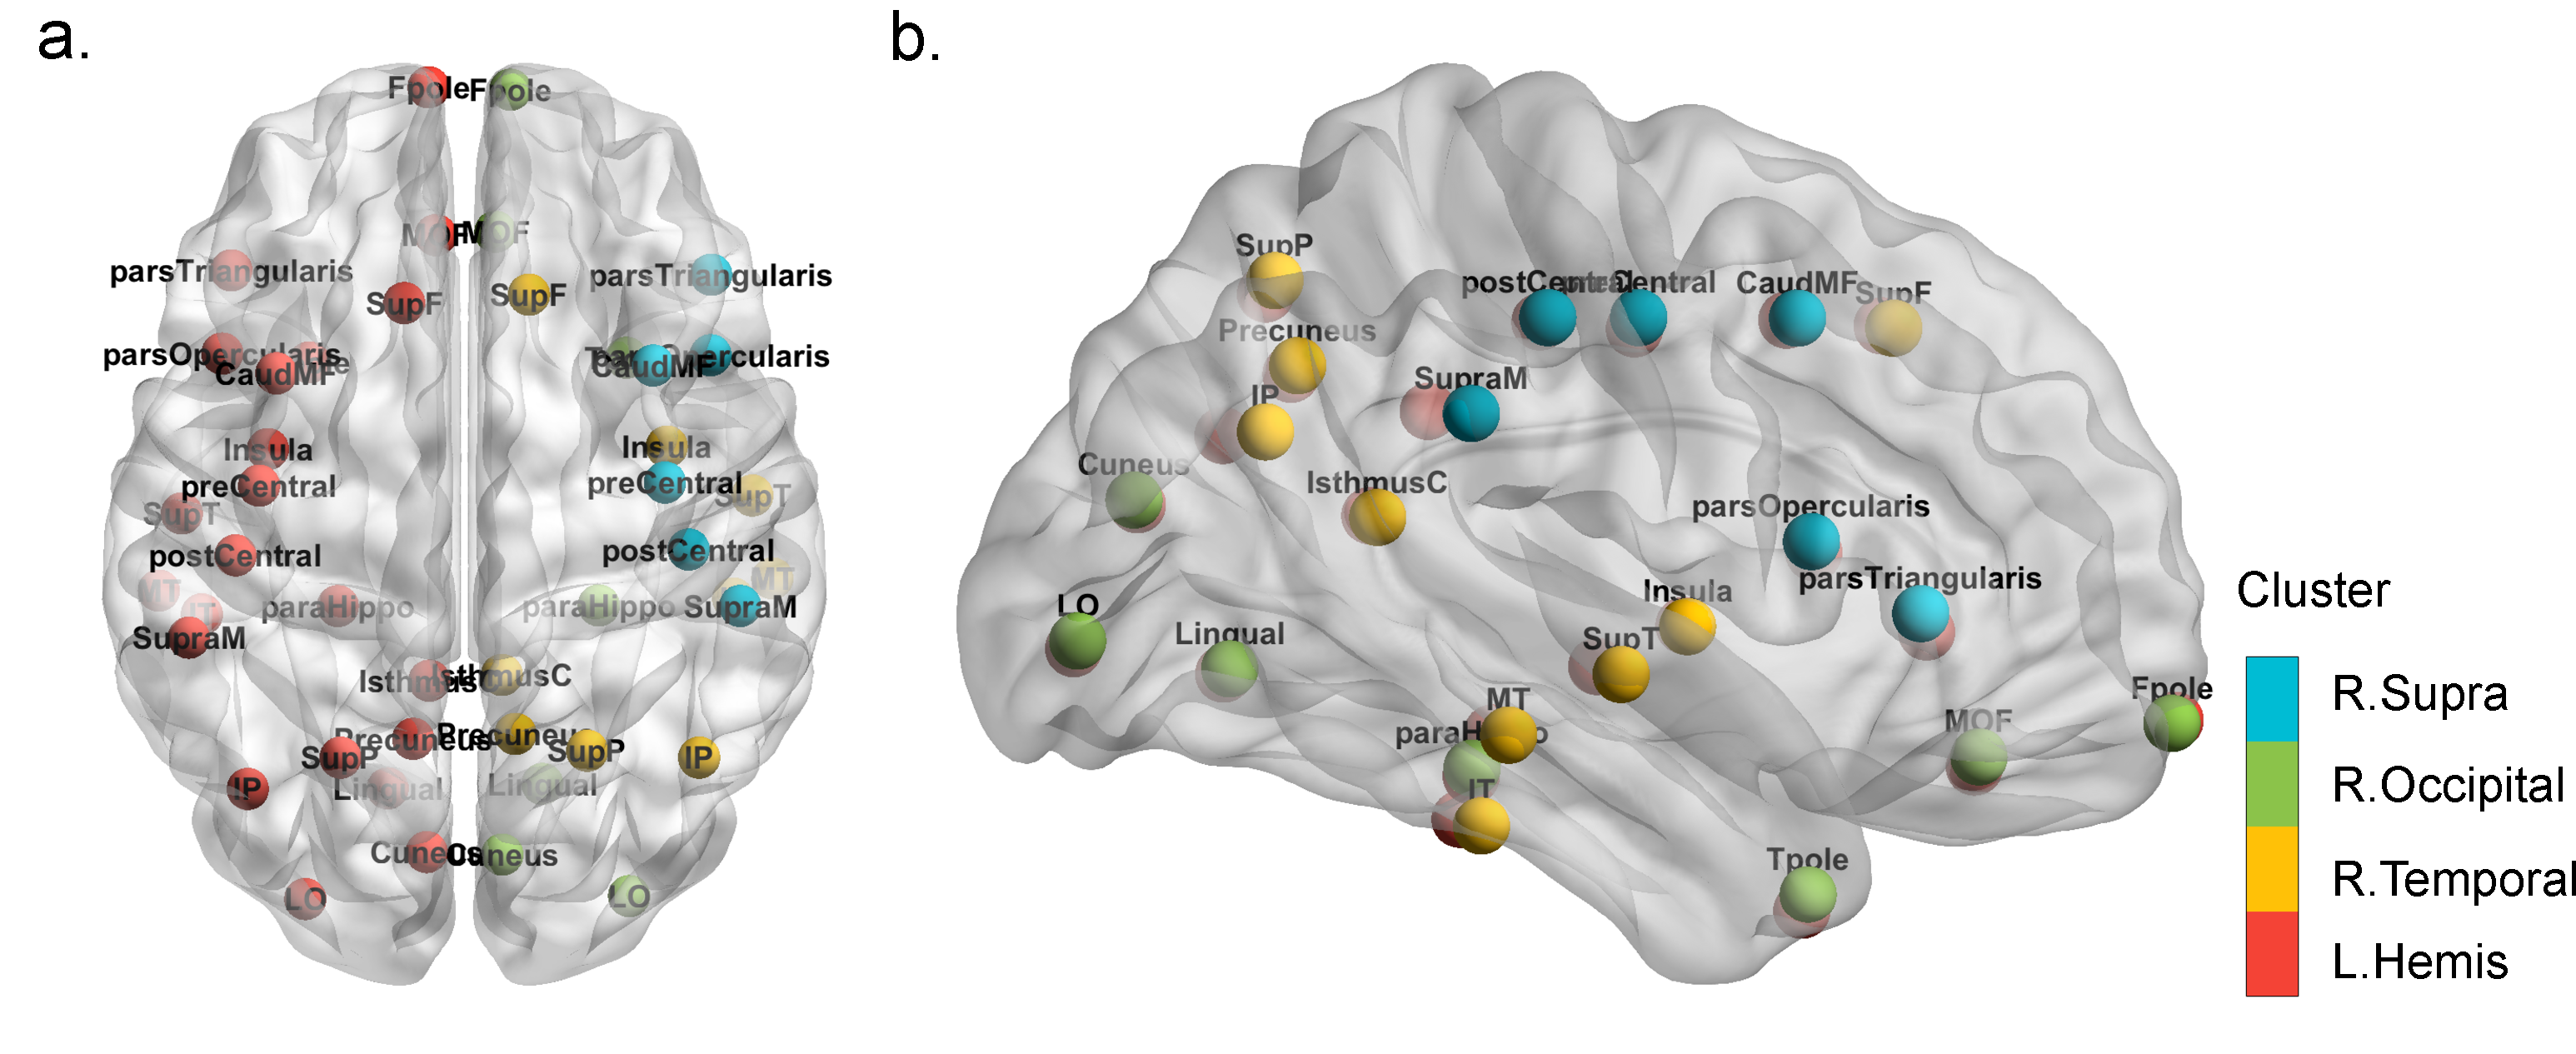
\includegraphics[width = .8\columnwidth]{brain_node_cluster.pdf}
    \caption{Illustration of brain node clustering results for HCP data with (a) top and (b) side views. }
    \label{fig:cluster_brain}
\end{figure}

\begin{figure*}[htb]
    \centering
    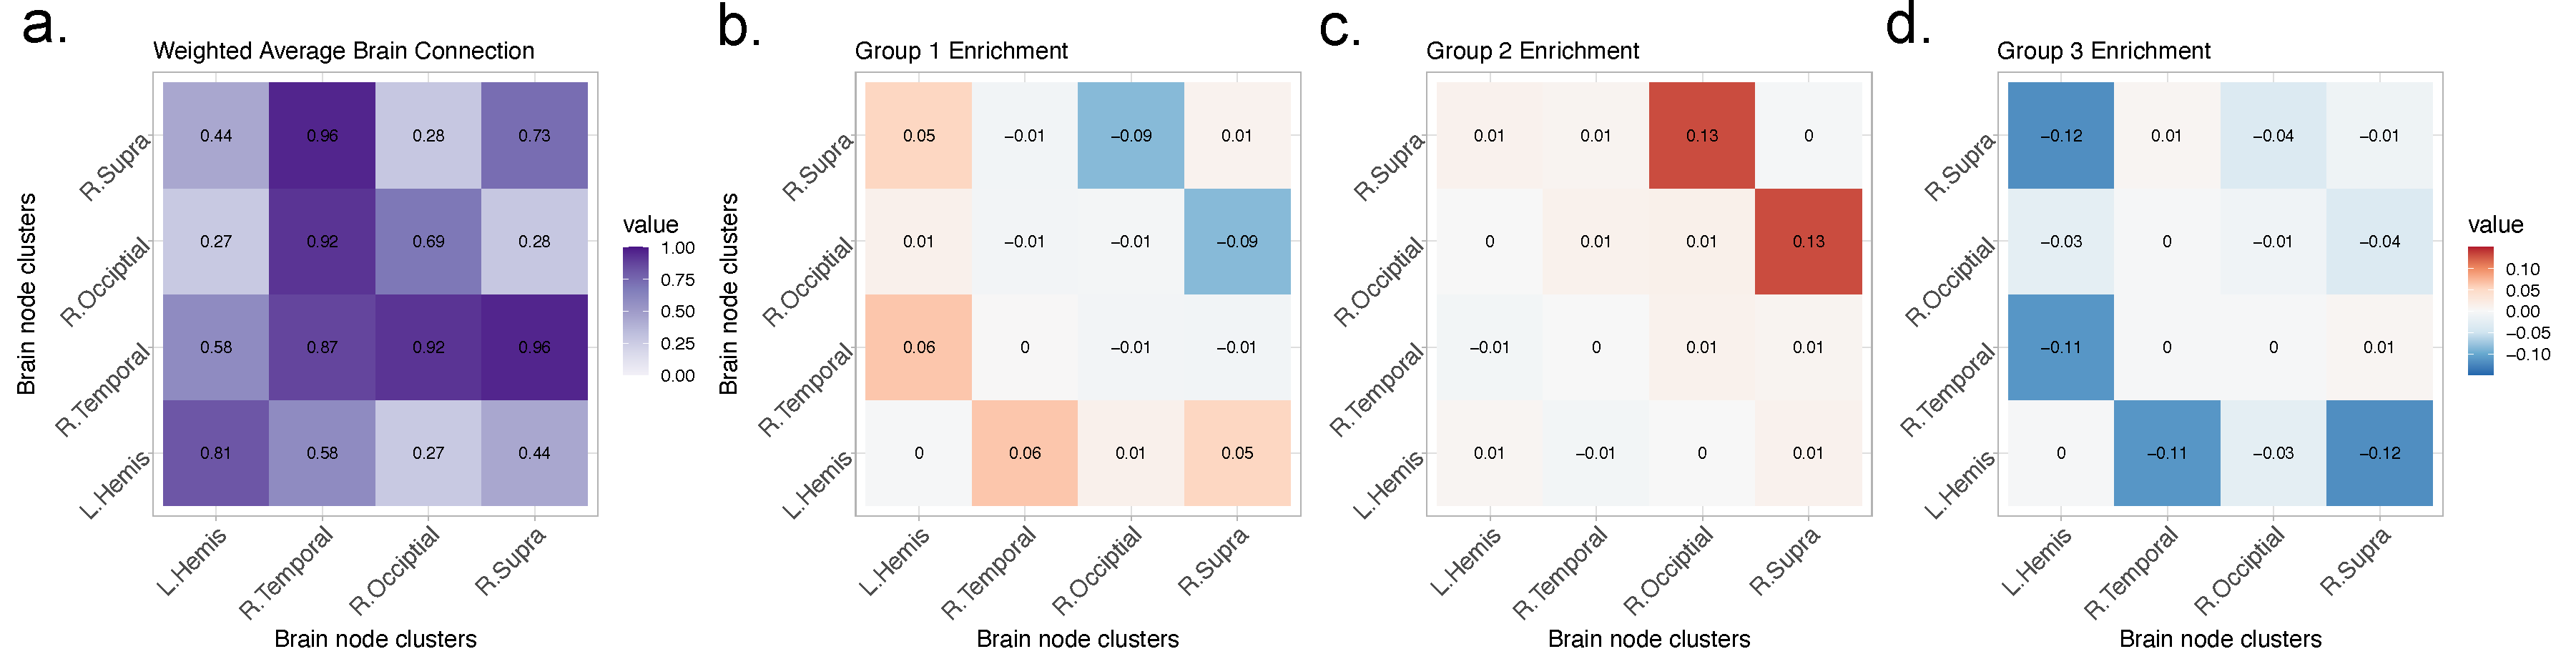
\includegraphics[width = 1\textwidth]{est_S_anno.pdf}
    \caption{Mode 3 slices of estimated core tensor $\hat \tS$. (a) Average estimated slice weighted by the group size; (b)-(d) Group-specified enrichment, i.e., the \DIFdelbeginFL \DIFdelFL{subtraction }\DIFdelendFL \DIFaddbeginFL \DIFaddFL{difference }\DIFaddendFL between each slice of $\hat \tS$ and the averaged slice. }
    \label{fig:ests}
\end{figure*}

\begin{figure*}[htb]
    \centering
    \includegraphics[width = 1\textwidth]{brain_connection.pdf}
    \caption{Observed brain connections in the population and each group of individuals. (a) Average brain network; (b)-(d) Group-specified brain \DIFdelbeginFL \DIFdelFL{networks enrichment }\DIFdelendFL \DIFaddbeginFL \DIFaddFL{network enrichments }\DIFaddendFL in Groups 1-3. Red edges \DIFdelbeginFL \DIFdelFL{refer to }\DIFdelendFL \DIFaddbeginFL \DIFaddFL{represent }\DIFaddendFL the positive enrichment and blue edges \DIFdelbeginFL \DIFdelFL{refer }\DIFdelendFL \DIFaddbeginFL \DIFaddFL{represent }\DIFaddendFL the negative \DIFdelbeginFL \DIFdelFL{reduction}\DIFdelendFL \DIFaddbeginFL \DIFaddFL{enrichment}\DIFaddendFL .}
    \label{fig:brain_conn}
\end{figure*}

Figure~\ref{fig:ests} illustrates the estimated core tensor $\hat \tS$ with estimated clustering, and Figure~\ref{fig:brain_conn} visualizes the average \DIFdelbegin \DIFdel{observed }\DIFdelend brain connections and the connection enrichment \DIFdelbegin \DIFdel{with average observed }\DIFdelend \DIFaddbegin \DIFadd{in contrast to average }\DIFaddend networks in each group. In general, we find that the inner-hemisphere connection has stronger connection compared to inter-hemisphere connections (Figure~\ref{fig:ests}a). Also, the back and front parts (\emph{R.Occipital}, \emph{R.Supra}) are shown to have more interactions with temporal tissues than inner-cluster connections. In addition, the group 1 with 54\% females \DIFdelbegin \DIFdel{implies }\DIFdelend \DIFaddbegin \DIFadd{shows }\DIFaddend an enrichment on the inter-hemisphere connections (Figure~\ref{fig:ests}b)\DIFaddbegin \DIFadd{, }\DIFaddend while group 4 with only 36\% females exhibits a reduction (Figure~\ref{fig:ests}d). This result agrees with previous findings in \cite{hu2021generalized}. The enrichment on the back-front connection is also recognized in group\DIFaddbegin \DIFadd{~}\DIFaddend 3 (Figure~\ref{fig:ests}c). The interpretive \DIFdelbegin \DIFdel{pattern in }\DIFdelend \DIFaddbegin \DIFadd{patterns in our }\DIFaddend results demonstrate the usefulness of our clustering methods in the human brain connectome data application. 


\subsection{Peru Legislation data analysis}

We also apply our method to the legislation networks in the Congress of the Republic of Peru \citep{lee2017time}. Because of the frequent political power shifts in the Peruvian Congress during 2006-2011, we choose to focus on the data for the first half of 2006-2007 year. The dataset records the co-sponsorship of 116 legislators from top 5 parties and 802 bill proposals. We reconstruct legislation network as an order-3 binary tensor $\tY \in \{0,1\}^{116 \times 116 \times 116}$, where $\tY_{ijk} = 1$ if the legislators $(i,j,k)$ have sponsored the same bill, and $\tY_{ijk} = 0$ otherwise. The true party affiliations of legislators are provided and serve as \DIFaddbegin \DIFadd{the }\DIFaddend ground truth. We apply various higher-order clustering methods to $\tY$ with $r = 5$. Table~\ref{tab:peru} shows that our \textbf{\small dTBM} achieves the best performance compared to others. The second best method is the two-stage algorithm \textbf{\small HLloyd}, followed by the spectral methods \textbf{\small SCORE} and \textbf{\small HOSVD+}. This result is consistent with our simulations under strong signal and moderate degree heterogeneity. The comparison suggests that our method \textbf{\small dTBM} is more appealing in real-world applications.

\begin{table}[ht]
    \centering
    \begin{tabular}{c |c  c cc c}
    \hline
        Method & \textbf{\small dTBM} 
        &\textbf{\small HOSVD}
        &\textbf{\small HOSVD+} & \textbf{\small HLloyd} &  \textbf{\small SCORE}\\
         CER & \textbf{0.116}
         &  0.22 
         &0.213 & 0.149 &0.199\\
         \hline
    \end{tabular}
    \caption{Clustering errors (measured by CER) for various methods in the analysis of Peru Legislation dataset.}
    \label{tab:peru}
\end{table}



\DIFdelbegin \section{\DIFdel{Conclusion}}%DIFAUXCMD
\addtocounter{section}{-1}%DIFAUXCMD
%DIFDELCMD < \label{sec:con}
%DIFDELCMD < %%%
\DIFdel{We have developed a general degree-corrected tensor block model with a two-step angle-based polynomial-times algorithm. We have, for the first time, characterized the statistical and computational behaviors of the degree-corrected tensor block model under different signal-to-noise ratio regimes. Simulations and Peru Legislation and Human brain connection data analysis confirm the potential of our method for practical applications.
}%DIFDELCMD < 

%DIFDELCMD < %%%
%DIF <  {\color{red}
%DIF <  Future direction. 
%DIF <  \begin{enumerate}
%DIF <      \item Missing data.
%DIF <      \item Sub-exponential data.
%DIF <      \item Imbalance in community size and heterogeneity.
%DIF <  \end{enumerate}
%DIF <  }
%DIFDELCMD < 

%DIFDELCMD < {
%DIFDELCMD < \color{blue}
%DIFDELCMD < 

%DIFDELCMD < %%%
\DIFdelend \section{Proof Sketches}\DIFaddbegin \label{sec:mainproof}
\DIFaddend 

In this section, we provide the proof sketches for \DIFdelbegin \DIFdel{Theorem~\ref{thm:initial}and Theorem~}\DIFdelend \DIFaddbegin \DIFadd{the main Theorems~\ref{thm:initial}-}\DIFaddend \ref{thm:refinement}. Detail proofs \DIFaddbegin \DIFadd{and extra theoretical results }\DIFaddend are provided in Appendix.


\subsection{Proof sketch of Theorem~\ref{thm:initial}}
The proof of Theorem~\ref{thm:initial} is \DIFdelbegin \DIFdel{mainly }\DIFdelend inspired by the proof idea of \citet[Lemma 1]{gao2018community}\DIFdelbegin \DIFdel{, and extra difficulties due to }\DIFdelend \DIFaddbegin \DIFadd{. The extra difficulties are }\DIFaddend the angle gap \DIFdelbegin \DIFdel{assumption and tensor property are addressed in }\DIFdelend \DIFaddbegin \DIFadd{characterization and multilinear algebra property in tensors; we address both challenges in }\DIFaddend our proof. Specifically, we control the misclustering error by the estimation error of $\hat \tX$ calculated in Step \DIFdelbegin \DIFdel{2.  }\DIFdelend \DIFaddbegin \DIFadd{2 of Sub-algorithm~}\hyperref[alg:main]{1}\DIFadd{.  }\DIFaddend We prove the following inequality
\begin{equation}\label{eq:proof_4}
    \ell(z^{(0)},z) \lesssim \frac{1}{p}\min_{\pi \in \Pi} \sum_{i: z^{(0)}(i) \neq \pi(z(i))} \theta(i)^2 \lesssim \frac{\sigma^2 r^{K-1}}{ \Delta_{\min}^2 p^K} \onormSize{}{\hat \tX - \tX}_F^2 \lesssim \frac{r^K p^{-K/2}}{\text{SNR}},
\end{equation}
where \DIFdelbegin \DIFdel{$\tX = \bbE[\tY]$ }\DIFdelend \DIFaddbegin \DIFadd{$\tX = \bbE \tY$ }\DIFaddend is the true mean. The first inequality in~\eqref{eq:proof_4} holds with the assumption \DIFdelbegin \DIFdel{$\min_{i \in [p]} \theta(i) \geq c$ }\DIFdelend \DIFaddbegin \DIFadd{$\min_{i \in [p]} \theta(i) \geq c>0$ }\DIFaddend in Theorem~\ref{thm:initial}. The second inequality relies on \DIFdelbegin \DIFdel{the intermediate }\DIFdelend \DIFaddbegin \DIFadd{an important }\DIFaddend conclusion that the angle gap of mean tensor $\tX$ is lower bounded by \DIFdelbegin \DIFdel{a function }\DIFdelend \DIFaddbegin \DIFadd{that }\DIFaddend of core tensor \DIFaddbegin \DIFadd{$\tS$, i.e., the }\DIFaddend minimal angle gap $\Delta_{\min}$ defined in Assumption~\ref{assmp:min_gap}. Let $\ma^{s} \coloneqq \ma/\onorm{\ma}$ denote the normalized vector \DIFdelbegin \DIFdel{and make }\DIFdelend \DIFaddbegin \DIFadd{with }\DIFaddend the convention that $\ma^s = 0$ if $\ma = 0$. We \DIFaddbegin \DIFadd{want to }\DIFaddend show that
\begin{equation}\label{eq:proof_4_gap}
\min_{z(i) \neq z(j)} \onormSize{}{[\mX_{i:}]^s - [\mX_{j:}]^s} \gtrsim \Delta_{\min},
\end{equation}
where $\mX = \mat(\tX)$. The most challenging part in the proof of Theorem~\ref{thm:initial} lies in the derivation of inequality~\eqref{eq:proof_4_gap}, in which the proof of \cite{gao2018community} is no longer applicable due to different angle gap assumption in our dTBM. \DIFdelbegin \DIFdel{Extra }\DIFdelend \DIFaddbegin \DIFadd{We develop the extra }\DIFaddend padding technique in Lemma~\ref{lem:pad} and balance assumption~\eqref{eq:degree} \DIFdelbegin \DIFdel{are equipped }\DIFdelend to derive~\eqref{eq:proof_4_gap}. Last, we finish the proof of Theorem~\ref{thm:initial} by showing the third inequality \DIFdelbegin \DIFdel{with }\DIFdelend \DIFaddbegin \DIFadd{of~}\eqref{eq:proof_4} \DIFadd{using }\DIFaddend \citet[Proposition 1]{han2020exact}. 


\subsection{Proof sketch of Theorem 5}
The proof of Theorem~\ref{thm:refinement} is \DIFdelbegin \DIFdel{mainly }\DIFdelend inspired by the proof idea of \citet[Theorem 2]{han2020exact}\DIFdelbegin \DIFdel{, and extra polar coordinate based techniques are imposed due to }\DIFdelend \DIFaddbegin \DIFadd{. We develop extra polar-coordinate based techniques with angle gap characterization to address }\DIFaddend the nuisance degree heterogeneity\DIFdelbegin \DIFdel{and angle gap assumption. We conduct the contraction property of the }\DIFdelend \DIFaddbegin \DIFadd{. We introduce an intermediate quantity called }\DIFaddend misclustering loss
\begin{equation}
     L^{(t)} = \frac{1}{p}  \sum_{i \in [p]} \theta(i) \sum_{b \in [r]}  \ind \offf{ z^{(t)}(i) = b } \onorm{ \off{ \mS_{ z(i):}  }^s - \off{ \mS_{b:}  }^s  }^2,
\end{equation}
\DIFdelbegin \DIFdel{and }\DIFdelend \DIFaddbegin \DIFadd{where the superscript $\cdot^{s}$ denotes the normalized vector; i.e., $\ma^s:=\ma/\onorm{\ma}$ if $\ma\neq 0$ and $\ma^{s}=0$ if $\ma=0$ for any vector $\ma$. We show that $L^{(t)}$ provides an upper bound for the misclassification error of interest via the inequality $\ell^{(t)}\lesssim {L^{(t)}\over \Delta^2_{\min}}$. Therefore, it suffices to control $L^{(t)}$. Further, we }\DIFaddend introduce the oracle estimators for core tensor \DIFdelbegin \DIFdel{and assignment }%DIFDELCMD < \begin{equation}
%DIFDELCMD <     \tilde \tS = \tY \times_1 \mW^T \times_2 \cdots \times_K \mW^T, 
%DIFDELCMD <     %\quad \tilde z(i) = \argmin_{a \in [r]} \onormSize{}{ { [\mat(\tY)_{i:} \mV]^s - [\mat(\tilde \tS)_{a:}]^s } }^2
%DIFDELCMD < \end{equation}%%%
\DIFdelend \DIFaddbegin \DIFadd{under the true cluster assignment via 
}\begin{equation}
    \tilde \tS = \tY \times_1 \mW^T \times_2 \cdots \times_K \mW^T, 
\end{equation}\DIFaddend 
where \DIFdelbegin \DIFdel{$\mW = \mM \of{ \text{diag}(\ind_{p}^T \mM) }^{-1}$ }\DIFdelend \DIFaddbegin \DIFadd{$\mW = \mM \of{ \text{diag}(\mone_{p}^T \mM) }^{-1}$ }\DIFaddend is the weighted true membership matrix. Let $ \mV = \mW^{\otimes (K-1)}$ denote the Kronecker product of \DIFdelbegin \DIFdel{$K-1$ }\DIFdelend \DIFaddbegin \DIFadd{$(K-1)$ copies of }\DIFaddend $\mW$ matrices, and \DIFdelbegin \DIFdel{similarly define }\DIFdelend \DIFaddbegin \DIFadd{we define the $t$-th iteration quantities }\DIFaddend $\mW^{(t)}, \mV^{(t)}$ \DIFdelbegin \DIFdel{with $\mM^{(t)}$ corresponding to }\DIFdelend \DIFaddbegin \DIFadd{corresponding to $\mM^{(t)}$ (or equivalently }\DIFaddend $z^{(t)}$\DIFaddbegin \DIFadd{)}\DIFaddend . To evaluate $L^{(t+1)}$, we \DIFdelbegin \DIFdel{consider the event 
}%DIFDELCMD < \begin{equation}\label{eq:proof_5_event}
%DIFDELCMD <     \ind \offf{ z^{(t+1)}(i) = b } = \ind \offf{       \onormSize{}{ [ \mY_{i:} \mV^{(t)}  ]^s - [\mS_{b:}^{(t)}]^s }^2 \leq \onormSize{}{ [ \mY_{i:} \mV^{(t)}  ]^s - [\mS_{z(i):}^{(t)}]^s }^2} \leq A_{ib} + B_{ib}
%DIFDELCMD < \end{equation}%%%
\DIFdelend \DIFaddbegin \DIFadd{prove the bound
}\begin{equation}\label{eq:proof_5_event}
    \ind \offf{ z^{(t+1)}(i) = b } = \ind \offf{       \onormSize{}{ [ \mY_{i:} \mV^{(t)}  ]^s - [\mS_{b:}^{(t)}]^s }^2 \leq \onormSize{}{ [ \mY_{i:} \mV^{(t)}  ]^s - [\mS_{z(i):}^{(t)}]^s }^2} \leq A_{ib} + B_{ib},
\end{equation}\DIFaddend 
where $\mY = \mat(\tY)$, $ \mS = \mat(\tS)$, $\mS^{(t)} = \mat(\tS^{(t)})$ and
\begin{align}
        A_{ib} &= \ind \offf{\ang{ \mE_{i:} \mV, \off{  \tilde \mS_{z(i):} }^s - \off{  \tilde \mS_{b:} }^s } \lesssim -  \onorm{ \off{ \mS_{z(i):}  }^s - \off{ \mS_{b:}  }^s  }^2 },\\
        B_{ib} &= \ind \offf{\onorm{ \off{ \mS_{z(i):}  }^s - \off{ \mS_{b:}  }^s  }^2 \lesssim F_{ib}^{(t)} + G_{ib}^{(t)} + H_{ib}^{(t)} }.
\end{align}
The terms $F_{ib}^{(t)}, G_{ib}^{(t)}, H_{ib}^{(t)}$ are controlled by $z^{(t)}, \tS^{(t)}$\DIFdelbegin \DIFdel{, and detail definitions are }\DIFdelend \DIFaddbegin \DIFadd{; see the detailed definitions }\DIFaddend in \eqref{eq:f}, \eqref{eq:g}, \eqref{eq:h}. Note that the event $A_{ib}$ only involves the oracle estimator \DIFaddbegin \DIFadd{independent of $t$, }\DIFaddend while all the terms related to the $t$-th iteration \DIFdelbegin \DIFdel{estimator }\DIFdelend are in $B_{ib}$. Thus, the inequality~\eqref{eq:proof_5_event} decomposes the misclustering loss in the $(t+1)$-th iteration \DIFdelbegin \DIFdel{by }\DIFdelend \DIFaddbegin \DIFadd{into }\DIFaddend the oracle loss and the loss in $t$-th iteration. This decomposition leads to the separation of statistical error and computational error in the final upper bound of Theorem~\ref{thm:refinement}.

Specifically, we prove the contraction inequality
\begin{equation}\label{eq:proof_5_ineq}
    L^{(t+1)} \lesssim \xi + \rho L^{(t)}, \quad \xi = \frac{1}{p}  \sum_{i \in [p]} \theta(i) \sum_{b \in [r]}  A_{ib} \onorm{ \off{ \mS_{ z(i):}  }^s - \off{ \mS_{b:}  }^s  }^2,
\end{equation}
where $\rho \in (0,1)$ is the contraction parameter, and we call $\xi$ the oracle loss. Controlling the probability of event $B_{ib}$ and obtaining the $\rho L^{(t)}$ term in the right hand side of~\eqref{eq:proof_5_ineq} \DIFdelbegin \DIFdel{is the most tricky and challenging part }\DIFdelend \DIFaddbegin \DIFadd{are the most challenging parts }\DIFaddend in the proof of Theorem~\ref{thm:refinement}. Note that the true and estimated core tensors are involved \DIFdelbegin \DIFdel{as }\DIFdelend \DIFaddbegin \DIFadd{via their }\DIFaddend normalized rows such as $\mS_{a:}^s, \tilde \mS_{a:}^s, [\mS^{(t)}_{a:}]^s$. The Cartesian coordinate based analysis in \cite{han2020exact} is no longer applicable in our case. Instead, we use the \DIFdelbegin \DIFdel{polar coordinate }\DIFdelend \DIFaddbegin \DIFadd{polar-coordinate }\DIFaddend based analysis and the geometry property of trigonometric functions to derive the high probability upper bounds for $F_{ib}^{(t)}, G_{ib}^{(t)}, H_{ib}^{(t)}$. 

Further, by sub-Gaussian concentration, we prove the high probability upper bound for oracle loss
\begin{equation}\label{eq:proof_5_xi}
    \xi  \lesssim \exp\of{- \frac{p^{K-1}\text{SNR}}{r^{K-1}}}.
\end{equation}
Combining the decomposition~\eqref{eq:proof_5_ineq} and the oracle bound~\eqref{eq:proof_5_xi}, we finish the proof of Theorem~\ref{thm:refinement}.


\DIFdelbegin %DIFDELCMD < }
%DIFDELCMD < %%%
\DIFdelend \DIFaddbegin \section*{\DIFadd{Acknowledgments}}
\DIFadd{This research is supported in part by NSF grants DMS-1915978, DMS-2023239, EF-2133740, and funding from the Wisconsin Alumni Research foundation. We thank Zheng Tracy Ke, Rungang Han, Yuetian Luo for helpful discussions and for sharing software packages. 
}\DIFaddend 

\bibliographystyle{apalike}
\bibliography{tensor_wang}



%DIF < \section*{Appendices} 
\DIFdelbegin %DIFDELCMD < 

%DIFDELCMD < %%%
\DIFdelend \newpage
\appendix


We provide the proofs for all the theorems in our main paper. In each sub-section, we \DIFaddbegin \DIFadd{first }\DIFaddend show the proof of main theorem and \DIFdelbegin \DIFdel{attach }\DIFdelend \DIFaddbegin \DIFadd{then collect }\DIFaddend the useful lemmas in the end.

\section*{Notation}
Before the proofs, we first introduce the \DIFdelbegin \DIFdel{notations }\DIFdelend \DIFaddbegin \DIFadd{notation }\DIFaddend used throughout the \DIFdelbegin \DIFdel{following sections }\DIFdelend \DIFaddbegin \DIFadd{appendix }\DIFaddend and the generalized dTBM without symmetric assumptions\DIFdelbegin \DIFdel{for the proofs of Theorem~\ref{thm:unique} and Theorem~\ref{thm:stats}}\DIFdelend . The parameter space and minimal gap assumption \DIFdelbegin \DIFdel{for }\DIFdelend are also extended \DIFdelbegin \DIFdel{the generalized dTBM. The conclusions of Theorem~\ref{thm:unique} and \ref{thm:stats} in the main paper are obtained by simply setting $z_k = z, \mS_k = \mS, \mtheta_k = \mtheta, k \in [K]$ }\DIFdelend for the generalized dTBM. 

{\bf \DIFdelbegin \DIFdel{Notations}\DIFdelend \DIFaddbegin \DIFadd{Preliminaries}\DIFaddend .}
\DIFdelbegin %DIFDELCMD < \begin{enumerate}
%DIFDELCMD <     %%%
\DIFdelend \DIFaddbegin \begin{enumerate}[wide]
    \DIFaddend \item For \DIFdelbegin \DIFdel{all }\DIFdelend \DIFaddbegin \DIFadd{mode }\DIFaddend $ k \in [K]$, denote the \DIFdelbegin \DIFdel{tensor matricizations as
    }\DIFdelend \DIFaddbegin \DIFadd{mode-$k$ tensor matricizations by
    }\DIFaddend \begin{equation}
        \mY_k = \mat_k \of{ \tY }, \quad \mS_k = \mat_k \of{\tS}, \quad \mE_k = \mat_k \of{ \tE}, \quad \mX_k = \mat_k \of{\tX}.
    \end{equation}
    %DIF < We ignore the subscript $k$ when considering symmetric tensors. 
    \item For a vector $\ma$, let $\ma^{s} \coloneqq \ma/\onorm{\ma}$ denote the normalized vector. We make the convention that \DIFdelbegin \DIFdel{$\ma^s = 0$ if $\ma = 0$. 
    %DIF <  Then we rewrite the angle gap~\eqref{eq:general_minial_gap} as
    %DIF <  \begin{equation}
    %DIF <      \Delta_{\min} = \min_{k \in [K]} \min_{a \neq b \in [r_k]} \onorm{ \mS_{k,a:}^s - \mS_{k, b:}^s }.
    %DIF <  \end{equation}
    }\DIFdelend \DIFaddbegin \DIFadd{$\ma^s = {\bf 0}$ if $\ma = {\bf 0}$. 
    }\DIFaddend \item For a matrix \DIFdelbegin \DIFdel{$\mA \in \bbR^{n \times m} \in \bbR^{n^K \times m^K}$, let $\mA^{\otimes K}$ denotes the kronecker }\DIFdelend \DIFaddbegin \DIFadd{$\mA \in \bbR^{n \times m} $, let $\mA^{\otimes K}:=\mA\otimes \cdots \otimes \mA\in \bbR^{n^K \times m^K}$ denote the Kronecker }\DIFaddend product of $K$ \DIFdelbegin \DIFdel{matrices $\mA \otimes \cdots \otimes \mA$,
    }\DIFdelend \DIFaddbegin \DIFadd{copies of matrices $\mA $.
    }\DIFaddend \item For a matrix $\mA$, let $\onormSize{}{\mA}_\sigma$ denote the spectral norm of matrix $\mA$, which is equal to the maximal singular value of $\mA$; let $\lambda_k(\mA)$ denote the $k$-th largest singular value of $\mA$; let $\onormSize{}{\mA}_F$ denote the Frobenius norm of matrix $\mA$.
    \item For two \DIFdelbegin \DIFdel{terms }\DIFdelend \DIFaddbegin \DIFadd{sequence }\DIFaddend $a$ and $b$, let $a \asymp b$ if there exist two positive constants $c, C$ such that $cb \leq a\leq Cb$. 
\end{enumerate}


{\bf \DIFdelbegin \DIFdel{Generalized }\DIFdelend \DIFaddbegin \DIFadd{Model extension to generalized }\DIFaddend dTBM.} 

 The general order-$K$ $(p_1, \ldots, p_K)$-dimensional dTBM model with $r_k$ communities and degree heterogeneity $\mtheta_k = \entry{\theta_k(i)} \in \bbR_+^{p_k}$ is represented by
\begin{equation}\label{eq:general_dtbm}
    \tY = \tX+ \tE,\quad \text{where}\quad \tX=\tS \times_1 \mTheta_1 \mM_1 \times_2 \cdots \times_K \mTheta_K \mM_K,
\end{equation}
where $\tY \in \bbR^{p_1 \times \cdots \times p_K}$ is the data tensor, $\tX\in \mathbb{R}^{p_1\times \cdots \times p_K}$ is the mean tensor, $\tS \in \bbR^{r_1 \times \cdots \times r_K}$ is the core tensor, $\tE \in \bbR^{p_1 \times \cdots \times p_K}$ is the noise tensor consisting of independent \DIFdelbegin \DIFdel{mean-zero }\DIFdelend \DIFaddbegin \DIFadd{zero-mean }\DIFaddend sub-Gaussian entries with variance bounded by $\sigma^2$, $\mTheta_k = \text{diag}(\mtheta_k)$, and $\mM_k\in \{0,1\}^{p_k \times r_k}$ is the membership matrix corresponding to the assignment $z_k: [p_k] \mapsto [r_k]$, for all $k \in [K]$. 

For ease of notation, we use $\{z_k\}$ to denote the collection $\{z_k\}_{k=1}^K$, and $\{\mtheta_k\}$ to denote the collection $\{\mtheta_k\}_{k=1}^K$. Correspondingly, we consider the parameter space for the triplet $\of{\{z_k\}, \tS, \{\mtheta_k\}}$,

%DIF <  \begin{equation}\label{eq:general_family}
%DIF <      \tP (r)= \offf{ \of{\{z_k\}, \tS, \{\mtheta_k\}}: \mtheta_k \in\mathbb{R}^p_{+}, {c_1p\over r}\leq |z_k^{-1}(a)| \leq {c_2 p\over r}, c_3\leq \onorm{\mat_k(\tS)}_{a:}\leq c_4 , \onormSize{}{\mtheta_{z_k^{-1}(a)}}_1=|z_k^{-1}(a)|, a \in [r], k\in[K]}.
%DIF <  \end{equation}
\DIFdelbegin %DIFDELCMD < \footnotesize
%DIFDELCMD < \begin{align}
%DIFDELCMD <     \tP(\{r_k\}) = \Bigg\{ \of{\{z_k\}, \tS, \{\mtheta_k\}}:\  &\mtheta_k \in\mathbb{R}^p_{+}, {c_1 p_k\over r_k} |z_k^{-1}(a)| \leq {c_2 p_k\over r_k}, c_3 \leq  \onorm{\mS_{k,a:}} \leq c_4 ,\onormSize{}{\mtheta_{k,z_k^{-1}(a)}}_1=|z_k^{-1}(a)|, a \in [r_k], k\in[K]\Bigg\}. \label{eq:general_family}
%DIFDELCMD < \end{align}%%%
\DIFdelend \DIFaddbegin \begin{align}
 \tP(\{r_k\}) = \Bigg\{ &\of{\{z_k\}, \tS, \{\mtheta_k\}}:\\
   & \mtheta_k \in\mathbb{R}^p_{+}, {c_1 p_k\over r_k} |z_k^{-1}(a)| \leq {c_2 p_k\over r_k}, c_3 \leq  \onorm{\mS_{k,a:}} \leq c_4 ,\onormSize{}{\mtheta_{k,z_k^{-1}(a)}}_1=|z_k^{-1}(a)|, a \in [r_k], k\in[K]\Bigg\}. \label{eq:general_family}
\end{align}\DIFaddend 
\DIFdelbegin %DIFDELCMD < \normalsize
%DIFDELCMD < %%%
%DIF <  \begin{equation}
%DIF <      \tP = \offf{ \of{\{z_k\}, \tS, \{\mtheta_k\}}: \mtheta_k \in\mathbb{R}^p_{+}, |z_k^{-1}(a)| \asymp {p_k\over r_k},  \onorm{\mS_{k,a:}} \asymp 1 , \onormSize{}{\mtheta_{k,z_k^{-1}(a)}}_1=|z_k^{-1}(a)|, a \in [r], k\in[K]}.
%DIF <  \end{equation}
\DIFdelend 


We call the \DIFdelbegin \DIFdel{collection of }\DIFdelend degree heterogeneity $\{\mtheta_k\}$ is balanced if for all $k \in [K]$,
\begin{equation}\label{eq:general_balanced}
    {\min_{a\in[r]} \onormSize{}{\mtheta_{k, z_k^{-1}(a)}}=\left(1+o(1)\right)\max_{a\in[r]}\onormSize{}{\mtheta_{k,z_k^{-1}(a)}}}.
\end{equation}

We also consider the generalized Assumption~\ref{assmp:min_gap} on angle gap.
\begin{assumption}[Generalized angle gap]\label{assmp:general_minimal_gap} \DIFaddbegin \DIFadd{Recall $\mS_k=\mat_k(\tS)$. }\DIFaddend We assume the minimal gap between normalized rows of $\mS_k$ is bounded away from zero \DIFdelbegin \DIFdel{, }\DIFdelend \DIFaddbegin \DIFadd{for all $k\in[K]$; }\DIFaddend i.e.,
\DIFdelbegin %DIFDELCMD < \begin{equation}
%DIFDELCMD <      \Delta_{\min} \coloneqq \min_{k \in [K]} \min_{a \neq b \in [r_k]} \onorm{ \mS_{k,a:}^s - \mS_{k, b:}^s } > 0
%DIFDELCMD < \end{equation}%%%
\DIFdelend \DIFaddbegin \begin{equation}
     \Delta_{\min} \coloneqq \min_{k \in [K]} \min_{a \neq b \in [r_k]} \onorm{ \mS_{k,a:}^s - \mS_{k, b:}^s } > 0.
\end{equation}\DIFaddend 
\DIFdelbegin \DIFdel{for all $k \in [K]$. }\DIFdelend \DIFaddbegin \end{assumption}
\DIFaddend Similarly, let $\text{SNR} = \Delta_{\min}^2/\sigma^2$ with \DIFaddbegin \DIFadd{the }\DIFaddend generalized minimal gap $\Delta_{\min}^2$ \DIFaddbegin \DIFadd{defined }\DIFaddend in Assumption~\ref{assmp:general_minimal_gap}. We define the regime
\DIFdelbegin %DIFDELCMD < \begin{equation}
%DIFDELCMD <     \tP(\gamma) = \tP (\{r_k\}) \cap\{\tS \text{ satisfies $\text{SNR} = p^{\gamma}$ and $p_k \asymp p, k \in [K]$} \}.
%DIFDELCMD < \end{equation}%%%
\DIFdelend \DIFaddbegin \begin{equation}
    \tP(\gamma) = \tP (\{r_k\}) \cap\{\tS \text{ satisfies $\text{SNR} = p^{\gamma}$ and $p_k \asymp p, \text{for all }k \in [K]$} \}.
\end{equation}\DIFaddend 
\DIFdelbegin %DIFDELCMD < \end{assumption}
%DIFDELCMD < %%%
%DIF <  by extending the definition~\eqref{eq:minimal_gap} to asymmetric setting, 
%DIF <  \begin{equation}\label{eq:general_minial_gap}
%DIF <      \Delta_{\min} = \min_{k \in [K]} \min_{a \neq b \in [r_k]} \onorm{ \frac{ \of{\mat_k(\tS)}_{a:} }{ \onorm{\of{\mat_k(\tS)}_{a:}}} - \frac{ \of{\mat_k(\tS)}_{b:} }{ \onorm{\of{\mat_k(\tS)}_{b:} }} } > 0.
%DIF <  \end{equation}
\DIFdelend 



\section*{Proof of Theorem~\ref{thm:unique}}

\begin{proof}[Proof of Theorem~\ref{thm:unique}] 
%DIF < Recall that we prove Theorem~\ref{thm:unique} under the generalized dTBM~\eqref{eq:general_dtbm}. The identifiability for the symmetric dTBM~\eqref{eq:model_tensor} is indicated by simply setting $z_k = z, \mS_k = \mS, \mtheta_k = \mtheta, k \in [K]$.

To study the identifiability, we consider the noiseless model with $\tE = 0$. Assume there \DIFdelbegin \DIFdel{exists }\DIFdelend \DIFaddbegin \DIFadd{exist }\DIFaddend two parameterizations satisfying
\DIFdelbegin %DIFDELCMD < \begin{equation}\label{eq:another}
%DIFDELCMD <     \tX=\tS\times_1\Theta_1 \mM_1 \times_2 \cdots \times_K \Theta_K \mM'_K=\tS'\times_1\Theta'_1 \mM'_1 \times_2 \cdots \times_K \Theta'_K \mM'_K
%DIFDELCMD < \end{equation}%%%
\DIFdelend \DIFaddbegin \begin{equation}\label{eq:another}
    \tX=\tS\times_1\Theta_1 \mM_1 \times_2 \cdots \times_K \Theta_K \mM'_K=\tS'\times_1\Theta'_1 \mM'_1 \times_2 \cdots \times_K \Theta'_K \mM'_K,
\end{equation}\DIFaddend 
\DIFdelbegin \DIFdel{with }\DIFdelend \DIFaddbegin \DIFadd{where }\DIFaddend $\of{ \{z_k\}, \tS, \{ \mtheta_k \} } \in \tP(\{r_k\})$ and $\of{ \{z'_k\}, \tS', \{ \mtheta'_k \} } \in \tP(\{r_k'\})$ \DIFaddbegin \DIFadd{are two sets of parameters}\DIFaddend . We prove the sufficient and necessary conditions separately.

\DIFdelbegin %DIFDELCMD < \begin{enumerate}
%DIFDELCMD <     %%%
\DIFdelend \DIFaddbegin \begin{enumerate}[wide]
    \DIFaddend \item[$(\Leftarrow)$] For the necessity, it \DIFdelbegin \DIFdel{is equivalent to show that there exists a triplet $\of{ \{z'_k\}, \tS', \{ \mtheta'_k \} }$ is not identical to $\of{ \{z_k\}, \tS, \{ \mtheta_k \} }$ up to label permutation }\DIFdelend \DIFaddbegin \DIFadd{suffices to construct two distinct parameters up to cluster label permutation, }\DIFaddend if the model~\eqref{eq:general_dtbm} violates Assumption~\ref{assmp:general_minimal_gap}. Without loss of generality, we assume $\onorm{ \mS_{1,1:}^s - \mS_{1,2:}^s } = 0$.

 If $\mS_{1,1:}$ is a zero vector, \DIFdelbegin \DIFdel{consider }\DIFdelend \DIFaddbegin \DIFadd{construct }\DIFaddend $\mtheta_1'$ such that \DIFdelbegin \DIFdel{$\mtheta'_{z_1^{-1}(1)} \neq \mtheta_{z_1^{-1}(1)}$}\DIFdelend \DIFaddbegin \DIFadd{$\mtheta'_{1,z_1^{-1}(1)} \neq \mtheta_{1,z_1^{-1}(1)}$}\DIFaddend . Let $\{z'_k\} = \{z_k\}$, $\tS' = \tS$, and $\mtheta'_k = \mtheta_k$ for all $k = 2, \ldots, K$. Then the triplet $\of{ \{z'_k\}, \tS', \{ \mtheta'_k \} }$ is \DIFdelbegin \DIFdel{not identical to $\of{ \{z_k\}, \tS, \{ \mtheta_k \} }$ up to label permutation. We have a similar story when $\mS_{1,2:}$ is a zero vector. 
}%DIFDELCMD < 

%DIFDELCMD < %%%
\DIFdel{If neither $\mS_{1,1:}$ nor $\mS_{1,2:}$ is a zero vector, there exists a positive constant $c$ such that $\mS_{1,1:} = c \mS_{1,2:}$. Thus,there exists a core tensor $\tS_0 \in \bbR^{r_1 -1 \times \cdots \times r_K}$ such that 
}%DIFDELCMD < \begin{equation}
%DIFDELCMD <     \tS = \tS_0 \times_1 \mC \mR, \quad \text{where} \quad \mC = \text{diag}(1, c, 1,...,1) \in \bbR^{r_1 \times r_1}, \quad \mR = \begin{pmatrix}
%DIFDELCMD <     1& 0\\
%DIFDELCMD <     1&0 \\
%DIFDELCMD <     0 & \mone_{r_1-2}
%DIFDELCMD <     \end{pmatrix} \in \bbR^{r_1 \times (r_1 -1)}.
%DIFDELCMD < \end{equation}
%DIFDELCMD < %%%
\DIFdel{Let $\mD = \text{diag}(1+c, 1,...,1) \in \bbR^{r_1 -1 \times r_1 -1}$.Consider the parameterization
}%DIFDELCMD < \begin{equation}
%DIFDELCMD <     \mM'_1 = \mM_1 \mR, \quad \tS' = \tS_0 \times_1 \mD, \quad \theta'_{1}(i) = \begin{cases}
%DIFDELCMD <     \frac{1}{1+c} \theta_{1}(i) & i \in z_{1}^{-1}(1)\\
%DIFDELCMD <      \frac{c}{1+c} \theta_{1}(i) & i \in z_{1}^{-1}(2)\\
%DIFDELCMD <      \theta_{1}(i) & \text{ otherwise }
%DIFDELCMD <     \end{cases},
%DIFDELCMD < \end{equation}
%DIFDELCMD < %%%
\DIFdel{and $\mM'_k = \mM_k, \mtheta'_k = \mtheta_k$ for all $k = 2, \ldots, K$.Then we have constructed a
triplet $\of{ \{z'_k\}, \tS', \{ \mtheta'_k \} }$ that is not identical to $\of{ \{z_k\}, \tS, \{ \mtheta_k \} }$ up to label permutation.}%DIFDELCMD < 

%DIFDELCMD < \item[$(\Rightarrow)$] %%%
\item[\DIFdel{$(\Rightarrow)$}]%DIFAUXCMD
\DIFdel{For the sufficiency,it is equivalent to show that all possible triplets $\of{ \{z'_k\}, \tS', \{ \mtheta'_k \} }$ are identical to $\of{ \{z_k\}, \tS, \{ \mtheta_k \} }$ up to label permutation if the model~}%DIFDELCMD < \eqref{eq:general_dtbm} %%%
\DIFdel{satisfies Assumption~}%DIFDELCMD < \eqref{assmp:general_minimal_gap}%%%
\DIFdel{. We show the uniqueness of the parameters separately.
}%DIFDELCMD < 

%DIFDELCMD < %%%
%DIF < Suppose $(\tS', \mM', \Theta') $ satisfies assumption~\ref{eq:gap}. We want to show the decomposition~\eqref{eq:degree} is unique up to permutation. 
%DIFDELCMD < 

%DIFDELCMD < %%%
\DIFdel{First, we show the uniqueness of $\mM_k$ for all $k \in [K]$. Specifically, we show the uniqueness of the first mode membership matrix, i.e., $\mM'_1 = \mM_1\mP_1$ where $\mP_1$ is a permutation matrix. The uniqueness of $\mM_k$ for $k = 2,\ldots, K$ can be showed in the same way, and we omit the repeated procedures.
}%DIFDELCMD < 

%DIFDELCMD < %%%
\DIFdel{On one hand, consider the pair of nodes $(i,j)$ such that $z_1(i) = z_1(j)$. We have $\onormSize{}{\mX_{1, z_1(i):}^s - \mX_{1, z_1(j):}^s } = 0$ and thus $\onormSize{}{ (\mS')_{1, z'_1(i):}^{s} - (\mS')_{1, z'_1(j):}^{s} } = 0$ by Lemma~\ref{lem:angle}. Then, by Assumption~}%DIFDELCMD < \eqref{assmp:general_minimal_gap}%%%
\DIFdel{, we have $z'_1(i) = z'_1(j)$. On the other hand, consider the pair of nodes $(i,j)$ such that $z_1(i) \neq z_1(j)$. We have $ \onorm{\mX_{1,i:}^s - \mX_{1,j:}^s} \neq 0$ and thus $\onorm{ (\mS')_{1, z'_1(i):}^{s} - (\mS')_{1, z'_1(j):}^{s} } \neq 0$ by Lemma~\ref{lem:angle}. Hence, we have $z'_1(i) \neq z'_1(j)$. Therefore, we have proven that $z'_1$ is equal to $z_i$ up to label permutation.
}%DIFDELCMD < 

%DIFDELCMD < %%%
\DIFdel{Next, we show the uniqueness of $\mtheta_k$ for all $k \in [K]$ given that $z_k = z_k'$. Similarly, we show the detailed proof of the uniqueness of $\mtheta_1$, i.e.,$\mtheta'_1 = \mtheta_1$, and omit the repeated procedures for $\mtheta_k, k = 2,\ldots, K$}\DIFdelend \DIFaddbegin \DIFadd{distinct from }\of{ \{z_k\}, \tS, \{ \mtheta_k \} }\DIFadd{$ up to label permutation. Similar conclusion holds when $}\mS\DIFadd{_{1,2:}$ is a zero vector. 

If neither $}\mS\DIFadd{_{1,1:}$ nor $}\mS\DIFadd{_{1,2:}$ is a zero vector, there exists a positive constant $c$ such that $}\mS\DIFadd{_{1,1:} = c }\mS\DIFadd{_{1,2:}$. Thus, there exists a core tensor $}\tS\DIFadd{_0 \in }\bbR\DIFadd{^{r_1 -1 \times \cdots \times r_K}%
\mbox{%DIFAUXCMD
$ such that 
\begin{equation}
    \tS = \tS_0 \times_1 \mC \mR, \quad \text{where} \quad \mC = \text{diag}(1, c, 1,...,1) \in \bbR^{r_1 \times r_1}, \quad \mR = \begin{pmatrix}
    1& 0\\
    1&0 \\
    0 & \mone_{r_1-2}
    \end{pmatrix} \in \bbR^{r_1 \times (r_1 -1)}.
\end{equation}
Let $
}%DIFAUXCMD
}\mD \DIFadd{= \text{diag}(1+c, 1,}\DIFaddend .\DIFdelbegin %DIFDELCMD < 

%DIFDELCMD < %%%
\DIFdel{Consider an arbitrary $j \in [p_1]$ such that $z_1(j) = a$. Then for all the node $i \in  z_1^{-1}(a)$ in the same cluster of $j$, we have 
}%DIFDELCMD < \begin{equation}
%DIFDELCMD <     \frac{\mX_{1,z_1(i):}}{\mX_{1,z_1(j):}} = \frac{\mX'_{1,z_1(i):}}{\mX'_{1,z_1(j):}}, \text{ which implies }  \frac{\theta_1(j)}{\theta_1(i)} = \frac{\theta'_1(j)}{\theta'_1(i)}.\label{eq:theta_uniq}
%DIFDELCMD < \end{equation}
%DIFDELCMD < %%%
\DIFdel{Let $\theta'_1(j) = c\theta_1(j)$ for some constant $c$. By the equation~}%DIFDELCMD < \eqref{eq:theta_uniq}%%%
\DIFdel{, we have $\theta'_1(i) = c \theta_1(i)$ for all $ i \in  z_1^{-1}(a)$. Note that $(\{z_k\}, \tS', \{\mtheta'_k\}) \in \tP(\{r_k\})$. We have 
}%DIFDELCMD < \begin{equation}
%DIFDELCMD <     \sum_{j \in z^{-1}(a)} \theta'_1(j) = c \sum_{j \in z^{-1}(a)} \theta_1(j) = 1,
%DIFDELCMD < \end{equation}
%DIFDELCMD < %%%
\DIFdel{which implies $c = 1$. Hence, we have proven $\mtheta_1 = \mtheta'_1$ given that $z_1 = z'_1$}\DIFdelend .\DIFdelbegin %DIFDELCMD < 

%DIFDELCMD < %%%
\DIFdel{Last, we show the uniqueness of $\tS$, i.e., $\tS'=\tS\times_1 \mP^{-1}_1\times_2\cdots \times_K \mP^{-1}_K$, where $\mP_k, k \in [K]$ are permutation matrices.  Given $z'_k = z_k, \mtheta'_k = \mtheta_k$, we have $\mM'_k = \mM_k \mP_k$ and $\mTheta'_k = \mTheta_k$ for all $k \in [K]$}\DIFdelend .\DIFdelbegin %DIFDELCMD < 

%DIFDELCMD < %%%
\DIFdel{Let $\mD_k = \off{ (\mTheta'_k \mM'_k)^T (\mTheta'_k \mM'_k) }^{-1} (\mTheta'_k \mM'_k)^T, k \in [K]$. By the parameterization, we have 
}%DIFDELCMD < \begin{align}
%DIFDELCMD <     \tS' &= \tX \times_1 \mD_1 \times_2 \cdots \times_K \mD_K \\
%DIFDELCMD <     &= \tS \times_1 \mD_1 \mTheta_1 \mM_1 \times_1 \cdots \times_K \mD_K \mTheta_K \mM_K \\
%DIFDELCMD <     &= \tS \times_1 \mP^{-1}_1 \times_2 \cdots \times_K \mP^{-1}_K.
%DIFDELCMD < \end{align}
%DIFDELCMD < 

%DIFDELCMD < \end{enumerate}
%DIFDELCMD < 

%DIFDELCMD < %%%
\DIFdel{Therefore, we finish the proof of Theorem~\ref{thm:unique}.
}%DIFDELCMD < \end{proof}
%DIFDELCMD < 

%DIFDELCMD < {\bf %%%
\DIFdel{Useful Lemma for the Proof of Theorem~\ref{thm:unique}}%DIFDELCMD < } 
%DIFDELCMD < 

%DIFDELCMD < \begin{lem}[Motivation of angle-based clustering]\label{lem:angle} %%%
\DIFdel{Consider the signal tensor $\tX$ in the generalized dTBM~}%DIFDELCMD < \eqref{eq:general_dtbm} %%%
\DIFdel{with $(\{z_k\},\tS,\{\mtheta_k\})\in \tP(\{r_k\})$ and $r_k \geq 2$. Then, for any $k \in [K]$ and index pair $(i,j)\in[p_k]^2$, we have 
}%DIFDELCMD < \begin{equation}
%DIFDELCMD <     \onorm{ \mS_{k,z_k(i):}^s -  \mS_{k,z_k(j):}^s } = 0 \quad \text{if and only if} \quad \onorm{  \mX_{k, z_k(i):}^s -  \mX_{k,z_k(j):}^s } = 0.
%DIFDELCMD < \end{equation}
%DIFDELCMD < \end{lem}
%DIFDELCMD < 

%DIFDELCMD < \begin{proof}[Proof of Lemma~\ref{lem:angle}] %%%
\DIFdel{For simplicity, we show the detailed proof for $k = 1$ and drop the subscript $k$ in $\mX_k, \mS_k$.The repeated proofs for $k = 2, \ldots, K$ are omitted. 
}%DIFDELCMD < 

%DIFDELCMD < %%%
\DIFdel{By tensor matricization, we have
}%DIFDELCMD < \begin{equation}
%DIFDELCMD <     \mX_{j:} = \theta_1(j) \mS_{z_1(j):} \off{\mTheta_2 \mM_2 \otimes \cdots \otimes \mTheta_K \mM_K}^T.
%DIFDELCMD < \end{equation}     
%DIFDELCMD < %%%
\DIFdel{Let $\tilde \mM = \mTheta_2 \mM_2 \otimes \cdots \otimes \mTheta_K \mM_K$. Notice that for two vectors $\ma, \mb$ and two positive constants $c_1, c_2 >0$, we have
}%DIFDELCMD < \begin{equation}
%DIFDELCMD < \onorm{\ma^s - \mb^s} = \onorm{(c_1 \ma)^s - (c_2\mb)^s}.
%DIFDELCMD < \end{equation}
%DIFDELCMD < %%%
\DIFdel{Thus it is sufficient to show the following statement that for any index pair $(i,j)\in[p_1]^2$}\DIFdelend ,\DIFdelbegin %DIFDELCMD < \begin{equation}
%DIFDELCMD < \onorm{ \mS_{z_1(i):}^s - \mS_{z_1(j):}^s} = 0 \quad \text{if and only if} \quad \onorm{ \off{\mS_{z_1(i):} \tilde \mM^T }^s - \off{\mS_{z_1(j):}\tilde \mM^T}^s} = 0.
%DIFDELCMD < \end{equation}
%DIFDELCMD < \begin{enumerate}
\begin{enumerate}%DIFAUXCMD
%DIFDELCMD <     \item[$(\Leftarrow)$] %%%
\item[\DIFdel{$(\Leftarrow)$}]%DIFAUXCMD
\DIFdel{Suppose $\onorm{ \off{\mS_{z_1(i):} \tilde \mM^T }^s - \off{\mS_{z_1(j):}\tilde \mM^T}^s} = 0$. There exists a positive constant $c$ such that $\mS_{z_1(i):} \tilde \mM^T= c \mS_{z_1(j):} \tilde \mM^T$. Note that
}%DIFDELCMD < \begin{equation}
%DIFDELCMD <     \mS_{z_1(i):} = \mS_{z_1(i):} \tilde \mM^T \off{ \tilde \mM \of{ \tilde \mM^T  \tilde \mM}^{-1}},
%DIFDELCMD < \end{equation}
%DIFDELCMD < %%%
\DIFdel{where $ \tilde \mM^T  \tilde \mM$ is an invertiable diagonal matrix with positive diagonal elements. Thus, we have $ \mS_{z_1(i):} = c  \mS_{z_1(j):}$, which implies $ \onorm{  \mS_{z_1(i):}^s -  \mS_{z_1(j):}^s } = 0 $.
}%DIFDELCMD < 

%DIFDELCMD < \item[$(\Rightarrow)$] %%%
\item[\DIFdel{$(\Rightarrow)$}]%DIFAUXCMD
\DIFdel{Suppose $ \onorm{ \mS_{z_1(i):}^s - \mS_{z_1(j):}^s } = 0 $. There exists a positive constant $c$ such that $\mS_{z_1(i):} = c \mS_{z_1(j):}$, and thus $\mS_{z_1(i):} \tilde \mM^T = c \mS_{z_1(j):} \tilde \mM^T$, which implies $\onorm{\left[\mS_{z_1(i):} \tilde \mM^T\right]^s- \left[\mS_{z_1(j):} \tilde \mM^T\right]^s}=0$.
}
\end{enumerate}%DIFAUXCMD
%DIFDELCMD < \end{enumerate}
%DIFDELCMD < %%%
\DIFdel{Therefore, we finish the proof of Lemma~\ref{lem:angle}.
%DIF <  \begin{equation}
%DIF <      \tilde \mM^T \tilde \mM = \off{ \mM^T \Theta^2 \mM }^{\otimes K-1}, \quad \text{and} \quad \mM^T \Theta^2 \mM  = \text{diag} \of{ \sum_{j \in z^{-1}(1)} \theta(j)^2, ...,  \sum_{j \in z^{-1}(r)} \theta(j)^2}.
%DIF <  \end{equation}
}%DIFDELCMD < \end{proof}
%DIFDELCMD < 

%DIFDELCMD < %%%
\section*{\DIFdel{Proof of Theorem~\ref{thm:stats}}}
%DIFAUXCMD
%DIFDELCMD < 

%DIFDELCMD < \begin{proof}[Proof of Theorem~\ref{thm:stats}]
%DIFDELCMD < %%%
\DIFdel{We will prove a more general conclusion than the main paper by allowing growing $r_k$'s. Consider the generalized dTBM in the special case that $p_k = p$ and $r_k = r$ for all $ k\in [K]$. Specifically, we will show that, under 
the assumptions $K\geq 1$}\DIFdelend \DIFaddbegin \DIFadd{1) \in }\bbR\DIFadd{^{r_1 -1 \times r_1 -1}%
\mbox{%DIFAUXCMD
$. Consider the parameterization
\begin{equation}
    \mM'_1 = \mM_1 \mR, \quad \tS' = \tS_0 \times_1 \mD, \quad \theta'_{1}(i) = \begin{cases}
    \frac{1}{1+c} \theta_{1}(i) & i \in z_{1}^{-1}(1),\\
     \frac{c}{1+c} \theta_{1}(i) & i \in z_{1}^{-1}(2),\\
     \theta_{1}(i) & \text{ otherwise},
    \end{cases}
\end{equation}
and $
}%DIFAUXCMD
}\mM\DIFadd{'_k = }\mM\DIFadd{_k, }\mtheta\DIFadd{'_k = }\mtheta\DIFadd{_k$ for all $k = 2, \ldots, K$. Then we have constructed a
triplet $}\of{ \{z'_k\}, \tS', \{ \mtheta'_k \} }\DIFadd{$ that is distinct from $}\of{ \{z_k\}, \tS, \{ \mtheta_k \} }\DIFadd{$ up to label permutation. 

\item[\DIFadd{$(\Rightarrow)$}] For the sufficiency, it suffices to show that all possible triplets $}\of{ \{z'_k\}, \tS', \{ \mtheta'_k \} }\DIFadd{$ are identical to $}\of{ \{z_k\}, \tS, \{ \mtheta_k \} }\DIFadd{$ up to label permutation if the model~\eqref{eq:general_dtbm} satisfies Assumption~\eqref{assmp:general_minimal_gap}. We show the uniqueness of the three parameters, $\{}\mM\DIFadd{_k\}, \{}\tS\DIFadd{\}, \{}\mtheta\DIFadd{_k\}$ separately.

First, we show the uniqueness of $}\mM\DIFadd{_k$ for all $k \in }[\DIFadd{K}]\DIFadd{$. Without loss of generality, we consider $k=1$ and show the first mode membership matrix; i.e., $}\mM\DIFadd{'_1 = }\mM\DIFadd{_1}\mP\DIFadd{_1$ where $}\mP\DIFadd{_1$ is a permutation matrix. The conclusion for $k\geq 2$ can be showed similarly and thus omitted. 

Consider an arbitrary node pair $(i}\DIFaddend ,\DIFdelbegin \DIFdel{$r\lesssim p^{1/3}$ and SNR condition
}%DIFDELCMD < \[
%DIFDELCMD < {\Delta^2_{\min}\over \sigma^2}\lesssim {r^{K-1}\over p^{K-1}},\quad \text{or equivalently}, \quad \gamma\leq -(K-1)(1+\log_p r),
%DIFDELCMD < \]
%DIFDELCMD <  %%%
\DIFdel{the desired conclusion in Theorem~\ref{thm:stats} holds; i.e, for all $k \in [K]$, every estimator $\hat z_{k,\text{stat}}$ obeys
}%DIFDELCMD < \begin{equation}\label{eq:max}
%DIFDELCMD <     \sup_{(\{z_k\}, \tS, \{\mtheta_k\}) \in \tP(\gamma)} \bbE \left[ p\ell(\hat z_{k,\text{stat}}, z_k) \right]\geq 1.
%DIFDELCMD < \end{equation}
%DIFDELCMD < 

%DIFDELCMD <  %%%
\DIFdel{Noticed that inequality~}%DIFDELCMD < \eqref{eq:max} %%%
\DIFdel{is a minimax lower bound, it suffices to show the inequality holds for a particular $(\{z_k\}, \tS, \{\mtheta_k\}) \in \tP(\gamma)$. Specifically, we consider the estimation problem based on a particular parameter point $(\{z_k\}, \tS, \{\mtheta_k\})$ with the following three properties:
}%DIFDELCMD < \begin{equation}\label{eq:construction}
%DIFDELCMD <     \text{(i)}\  \theta_k(i)=1 \text{ for all }i\in[p]; \  \text{(ii)}\ % \onorm{{\mS_1\over \onormSize{}{\mS_1}}-{\mS_2\over \onormSize{}{\mS_2}}}=
%DIFDELCMD <     \Delta_{\min}\lesssim  \left({p\over r}\right)^{-\frac{K-1}{2}}\sigma; \  \text{(iii)}\ |z^{-1}_k(a)|={p \over r} \in \mathbb{Z}_+ \text{ for all }a\in[r],
%DIFDELCMD < \end{equation}
%DIFDELCMD < %%%
\DIFdel{for all $k \in [K]$.
%DIF <  \begin{enumerate}[label=(\roman*)]\label{eq:construction}
%DIF <  \item $\theta(i)=1 \text{ for all }i\in[p]$.
%DIF <  \item $\onorm{{\mS_1\over \onormSize{}{\mS_1}}-{\mS_2\over \onormSize{}{\mS_2}}}=\Delta_{\min}\lesssim \left({p\over r}\right)^{-(K-1)/2}\sigma$.
%DIF <  \item $|z(a)|={p \over r} \text{ for all }a\in[r]$.
%DIF <  \end{enumerate}
Furthermore, we define a subset of indices $T_k \subset [p_k], k \in [K]$ in order to avoid the complication of label permutation. Based on \mbox{%DIFAUXCMD
\citet[Proof of Theorem 6]{han2020exact}}\hspace{0pt}%DIFAUXCMD
, we consider the minimax rate over the restricted family of $\hat z_k$'s for which the following three conditions are satisfied:
}%DIFDELCMD < \footnotesize
%DIFDELCMD < \begin{equation}
%DIFDELCMD <     \text{(iv)}\ \hat z_k(i)=z_k(i) \text{ for all }i\in T_k; \ \text{(v)} \ |T^c_k|\asymp {p\over r}; \ \text{(vi)}\ \min_{\pi\in \Pi}\sum_{i\in[p]}\ind\{\hat z_k(i) \neq \pi\circ z_k (i)\} = \sum_{i\in[p]}\ind\{\hat z_k(i) \neq  z_k (i)\},
%DIFDELCMD < \end{equation}
%DIFDELCMD < \normalsize
%DIFDELCMD < %%%
\DIFdel{for all $k \in [K]$.
%DIF <  \begin{enumerate}[label=(\roman*)]
%DIF <  \setcounter{enumi}{3}
%DIF <      \item $\hat z(i)=z(i)$ for all $i\in T$.
%DIF <      \item $|T^c|\asymp {p\over r}$.
%DIF <      \item $\min_{\pi\in \Pi}\sum_{i\in[p]}\ind\{\hat z(i) \neq \pi\circ z (i)\} = \sum_{i\in[p]}\ind\{\hat z(i) \neq  z (i)\}$.
%DIF <  \end{enumerate}
The construction of $T$ is precisely the same as \mbox{%DIFAUXCMD
\citet[Proof of Theorem 6]{han2020exact}}\hspace{0pt}%DIFAUXCMD
. 
Then, following the proof of~\mbox{%DIFAUXCMD
\citet[Theorem 2]{gao2018community}}\hspace{0pt}%DIFAUXCMD
, for all $k \in [K]$, we have
}%DIFDELCMD < \begin{equation}\label{eq:minimax}
%DIFDELCMD < \inf_{\hat z_k}\sup_{z_k}\bbE \ell(\hat z_k, z_k) \gtrsim {1\over r^3 |T^c_k|}\sum_{i\in T^c_k}\inf_{\hat z_k}\left\{\bbP[\hat z_k(i)=2|z_k(i)=1] + \bbP[\hat z_k(i)=1|z_k(i)=2] \right\},
%DIFDELCMD < \end{equation}
%DIFDELCMD < %%%
\DIFdel{where $\hat z_k, z_k$ on the left hand side denote the generic clustering functions in $\tP(\gamma)$, $z_k$ on the right hand side denotes a particular parameter satisfying properties (i}\DIFdelend \DIFaddbegin \DIFadd{j)$. If $z_1(i}\DIFaddend ) \DIFdelbegin \DIFdel{-(vi), and the infimum on the right hand side is taken over the restricted family of $\hat z$ satisfying (iv) -(vi). Here, the factor $r^3=r\cdot r^2$ in~}%DIFDELCMD < \eqref{eq:minimax} %%%
\DIFdel{comes from two sources: $r^2\asymp {r\choose 2}$ comes from the multiple testing burden for all pairwise comparisons among $r$ clusters, and another $r$ comes from the number of elements $|T^c_k|\asymp {p\over r}$ to be clustered. 
}%DIFDELCMD < 

%DIFDELCMD < %%%
\DIFdel{Next, we need to find the lower bound of the rightmost side in~}%DIFDELCMD < \eqref{eq:minimax}%%%
\DIFdel{. For simplicity, we only show the bound for the mode-1 case $k = 1$. We drop the subscripts $1$ in $z_1, T_1, \mS_1, \mtheta_1$ and omit the repeated procedures for the cases of $k = 2,\ldots, K$. 
}%DIFDELCMD < 

%DIFDELCMD < %%%
\DIFdel{We consider the hypothesis test based on model~}%DIFDELCMD < \eqref{eq:general_dtbm}%%%
\DIFdel{. First, we reparameterize the model under the construction~}%DIFDELCMD < \eqref{eq:construction}
%DIFDELCMD < \begin{equation}
%DIFDELCMD <     \mx_a = \off{\mat_1 \of{ \tS\times_2 \mM_2\times_3\cdots \times_K \mM_K  }}_{a:}, \quad \text{for all} \quad a \in [r],
%DIFDELCMD < \end{equation}
%DIFDELCMD < %%%
\DIFdel{where $\mx_a$'s are centroids in $\bbR^{p^{K-1}}$. Without loss of generality, we consider the lower bound for the summand in~}%DIFDELCMD < \eqref{eq:minimax} %%%
\DIFdel{for $i=1$. The analysis for other $i\in T^c$ are similar. For notational simplicity, we suppressed the subscript $i$ and write $\my, \theta, z$ in place of $\my_1, \theta_1$ and $z(1)$, respectively. The equivalent vector problem for assessing the summand in~}%DIFDELCMD < \eqref{eq:minimax} %%%
\DIFdel{is
}%DIFDELCMD < \begin{equation}\label{eq:z}
%DIFDELCMD < \my=\theta\mx_{z}+\me,
%DIFDELCMD < \end{equation}
%DIFDELCMD < %%%
\DIFdel{where $\theta\in\bbR_{+}$ and $z\in \{1,2\}$ are unknown parameters, $\mx_1,\mx_2\in\bbR^{p^{K-1}}$ are given centroids, and $\me\in\bbR^{p^{K-1}}$ consists of i.i.d.\ $N(0,\sigma^2)$ entries.  Then, we consider the hypothesis testing under the model~}%DIFDELCMD < \eqref{eq:z}%%%
\DIFdel{:
}%DIFDELCMD < \begin{equation}\label{eq:test}
%DIFDELCMD < H_0\colon z=1, \quad \text{v.s.}\quad H_\alpha\colon z=2.
%DIFDELCMD < \end{equation}
%DIFDELCMD < %%%
\DIFdel{Note that the profile log-likelihood with respect to $z$ is
}%DIFDELCMD < \[
%DIFDELCMD < \tL(z,  \theta(z);\my)\propto - \inf_{\theta>0}\onormSize{}{\my- \theta\mx_{z}}^2 \propto  \cos^2(\my, \mx_{z}) \ind\{ \langle \my,\mx_{z}\rangle  >0 \}, 
%DIFDELCMD < \]
%DIFDELCMD < %%%
\DIFdel{and the maximum likelihood estimators (MLE) of $\theta$ and $z$ are
}%DIFDELCMD < \begin{equation}\label{eq:MLE}
%DIFDELCMD <     \hat \theta_{\text{MLE}}= \hat \theta(\hat z_{\text{MLE}})={\langle \my,\mx_{\hat z_{\text{MLE}}}\rangle \over \onorm{\mx_{\hat z_{\text{MLE}}}}^2}\vee 0 , \quad 
%DIFDELCMD < \hat z_{\text{MLE}}= \argmax_{a\in\{1,2\}} \offf{\cos(\my,\ \mx_a)\vee 0}. 
%DIFDELCMD < \end{equation}
%DIFDELCMD < 

%DIFDELCMD < %%%
\DIFdel{Then, the decision rule $\hat z_{\text{MLE}} \in\{1,2\}$ based on profile log-likelihood ratio is defined as
}%DIFDELCMD < \begin{equation}\label{eq:ratio}
%DIFDELCMD < \hat z_{\text{MLE}}=
%DIFDELCMD < \begin{cases}
%DIFDELCMD < 1 & \text{if }\cos(\my,\mx_1)\geq  \cos(\my,\mx_2) \text{ and }\langle \my,\mx_1\rangle > 0, \\
%DIFDELCMD < 2 & \text{if }\cos(\my,\mx_1)<\cos(\my,\mx_2) \text{ and }\langle \my,\mx_2\rangle > 0,\\
%DIFDELCMD < \text{1 or 2 with equal probability} & \text{otherwise.}
%DIFDELCMD < \end{cases}
%DIFDELCMD < \end{equation}
%DIFDELCMD < 

%DIFDELCMD < %%%
\DIFdel{Neyman-Pearson Lemma implies
}%DIFDELCMD < \begin{align}\label{eq:lower}
%DIFDELCMD < &\inf_{\hat z}\left\{\bbP[\hat z=2|z=1] + \bbP[\hat z=1|z=2]\right\}= \bbP[\hat z_{\text{MLE}}=1|z=2]+\bbP[\hat z_{\text{MLE}}=2|z=1].
%DIFDELCMD < \end{align}
%DIFDELCMD < %%%
\DIFdel{By symmetric, it suffices to bound $\bbP[\hat z_{\text{MLE}}=1|z=2]$. Using~}%DIFDELCMD < \eqref{eq:ratio}%%%
\DIFdel{, we obtain
%DIF < \fixme{Jiaxin}{$\theta^* = \hat \theta_{\text{MLE}}$?}
}%DIFDELCMD < \begin{align}\label{eq:bound}
%DIFDELCMD < \bbP[\hat z_{\text{MLE}}=1|z=2]&= \bbP\left[ \cos(\theta\mx_2+\me,\mx_1)\geq  \cos(\theta\mx_2+\me, \mx_2) \text{ and } \langle \theta\mx_2+\me,\mx_1\rangle > 0  \right] \notag \\
%DIFDELCMD < &\stackrel{(*)}{\geq} \bbP \left[\left\langle \me, {\mx^s_1 -\mx^s_2\over\onorm{\mx^s_1- \mx^s_2}}  \right\rangle  \geq {\theta \over 2}\onormSize{}{\mx_2} \onormSize{}{\mx^s_1-\mx^s_2}\rangle\right]-\notag \\
%DIFDELCMD < &\hspace{1cm} \bbP\left[\langle \me, \mx^s_1\rangle \leq -{\theta \over 2}\onorm{\mx_2}\left(2-\onormSize{}{\mx^s_1-\mx^s_2}^2\right)\right]\notag \\
%DIFDELCMD < &\stackrel{(**)}{=}\Phi\left({\theta \over 2}\onorm{\mx_2}(2-\onormSize{}{\mx^s_1-\mx^s_2}^2) \right)-\Phi\left({\theta\over 2}\onorm{\mx_2}\onormSize{}{\mx^s_1-\mx^s_2} \right),
%DIFDELCMD < \end{align}
%DIFDELCMD < %%%
\DIFdel{where $\Phi(\cdot)$ denotes the CDF for standard normal distribution. Here step $(*)$ is based on the inequality $\bbP(A\cup B)\geq \bbP(A)-\bbP(B^c)$ and the identity $1-\langle \mx^s_1,\mx^s_2 \rangle={1\over 2}\onorm{\mx^s_1-\mx^s_2}^2$; and step $(**)$ is based on isotropic property of i .i.d.\ Gaussian distribution
}%DIFDELCMD < \[
%DIFDELCMD < \left\langle\me, {\mx^s_1-\mx^s_2\over \onorm{\mx^s_1-\mx^s_2}} \right\rangle \sim N(0, \sigma^2),\quad \langle \me, \mx^s_1 \rangle \sim N(0,\sigma^2).
%DIFDELCMD < \]
%DIFDELCMD < %%%
\DIFdel{By construction~}%DIFDELCMD < \eqref{eq:construction} %%%
\DIFdel{of $(\{z_k\}, \tS, \{\mtheta_k\})$ with three properties and lower bound $\min_{a\in[r]}\onorm{\mS_{a:}}\geq c_3$ in the definition of $\tP(\gamma)$, we have $\theta^*=1$, $\onorm{\mx_2}\geq \onorm{\mS_{2:}}\min_{a\in[r]}\onorm{\mtheta_{\mz^{-1}(a)}}^{K-1} \gtrsim \left(p \over r\right)^{(K-1)/2}$. Also, note that under the construction~}%DIFDELCMD < \eqref{eq:construction}
%DIFDELCMD < \begin{equation}
%DIFDELCMD <     \cos(\mx_1, \mx_2) = \frac{\and{\mx_1, \mx_2}}{\onorm{\mx_1} \onorm{\mx_2} } = \frac{(p/r)^{K-1} \ang{\mS_{1:}, \mS_{2:}}}{ \sqrt{(p/r)^{K-1} \onorm{\mS_{1:}}^2} \sqrt{(p/r)^{K-1} \onorm{\mS_{2:}}^2} } = \cos(\mS_{1:}, \mS_{2:}),
%DIFDELCMD < \end{equation}
%DIFDELCMD < %%%
\DIFdel{which implies $\onormSize{}{\mx^s_1-\mx^s_2} = \onormSize{}{\mS_{1:}^s-\mS_{2:}^s} = \Delta_{\min} \leq 1$. Therefore, the equation~}%DIFDELCMD < \eqref{eq:bound} %%%
\DIFdel{is lower bounded by
}%DIFDELCMD < \begin{equation}\label{eq:normal}
%DIFDELCMD < \bbP[\hat z_{\text{MLE}}=1|z=2] \geq \bbP\left[ \left({p\over r}\right)^{(K-1)/2}\Delta_{\min}\lesssim N(0,1)\lesssim  \left({p\over r}\right)^{(K-1)/2} \right]\geq C>0,
%DIFDELCMD < \end{equation}
%DIFDELCMD <  %%%
\DIFdel{where the existence of strictly positive constant $C$ is based on the SNR assumption~}%DIFDELCMD < \eqref{eq:construction}%%%
\DIFdel{. Combining~}%DIFDELCMD < \eqref{eq:minimax}%%%
\DIFdel{, }%DIFDELCMD < \eqref{eq:lower} %%%
\DIFdel{and~}%DIFDELCMD < \eqref{eq:normal} %%%
\DIFdel{yields
}%DIFDELCMD < \[
%DIFDELCMD < \inf_{\hat z_1}\sup_{(\{z_k\},\tS,\{\mtheta_k\})\in \tP(\gamma)}\bbE\ell(\hat z_1, z_1)\gtrsim C>0, 
%DIFDELCMD < \]
%DIFDELCMD < %%%
\DIFdel{and henceforth for all $k \in [K]$
}%DIFDELCMD < \[
%DIFDELCMD < \inf_{\hat z_k}\sup_{(\{z_k\},\tS,\{\mtheta_k\})\in \tP(\gamma)}\bbE \left[p\ell(\hat z_k, z_k)\right]\geq 1.
%DIFDELCMD < \]
%DIFDELCMD < 

%DIFDELCMD < \end{proof}
%DIFDELCMD < 

%DIFDELCMD < %%%
\section*{\DIFdel{Proof of Theorem~\ref{thm:comp}}}
%DIFAUXCMD
%DIFDELCMD < 

%DIFDELCMD < \begin{proof}[Proof of Theorem~\ref{thm:comp}]
%DIFDELCMD < %%%
\DIFdel{The idea of proving computational hardness is to show the computational lower bound for aspecial class of degree-corrected tensor clustering model with $K\geq 2$. We construct the following special class of higher-order degree-corrected tensor clustering  model. For a given signal level $\gamma\in\bbR$ and noise variance $\sigma$, define a rank-2 symmetric tensor $\tS\in\bbR^{3\times \cdots\times 3}$ subject to
}%DIFDELCMD < \begin{equation}\label{eq:S}
%DIFDELCMD < \tS=\tS(\gamma) = \begin{bmatrix}
%DIFDELCMD < 		1\\
%DIFDELCMD < 		1\\
%DIFDELCMD < 		1
%DIFDELCMD < 		\end{bmatrix}^{\otimes K}
%DIFDELCMD < +\sigma p^{-\gamma/2} \begin{bmatrix}
%DIFDELCMD < 		1\\
%DIFDELCMD < 		-1\\
%DIFDELCMD < 		0
%DIFDELCMD < 	\end{bmatrix}^{\otimes K}.
%DIFDELCMD < \end{equation}
%DIFDELCMD < %%%
\DIFdel{Then, we consider the signal tensor family
}%DIFDELCMD < \begin{align}
%DIFDELCMD < \tP_{\text{shifted}}(\gamma)=\{\tX\colon & \tX=\tS\times_1\mM_1\times_2 \cdots \times_K\mM_K,\  \text{$\mM_k\in\{0,1\}^{p\times 3}$ is a membership matrix that}
%DIFDELCMD < \\
%DIFDELCMD < & \text{satisfies $|\mM_k(\colon,i)|\asymp p$ for all $i\in[3]$ and $k\in[K]$}\}.
%DIFDELCMD < \end{align}
%DIFDELCMD < %%%
\DIFdel{We claim that the constructed family satisfies the following two properties:
}%DIFDELCMD < \begin{enumerate}[wide,label=(\roman*)]
%DIFDELCMD <     \item %%%
\item%DIFAUXCMD
\DIFdel{For every $\gamma\in \mathbb{R}$, $\tP_{\text{shifted}}(\gamma)\subset \tP(\gamma)$, where $\tP(\gamma)$ is the degree-corrected cluster tensor family~}%DIFDELCMD < \eqref{eq:gammafamily}%%%
\DIFdel{.
    }%DIFDELCMD < \item %%%
\item%DIFAUXCMD
\DIFdel{For every $\gamma\in \mathbb{R}$, $\{\tX-1\colon \tX\in \tP_{\text{shifted}}(\gamma)\}\subset \tP_{\text{non-degree}}(\gamma)$, where $\tP_{\text{non-degree}}(\gamma)$ denotes the sub-family of rank-one tensor block model constructed in the proof of \mbox{%DIFAUXCMD
\citet[Theorem 7]{han2020exact}}\hspace{0pt}%DIFAUXCMD
. 
}%DIFDELCMD < \end{enumerate}
%DIFDELCMD < %%%
\DIFdel{The verification of the above two properties is provided in the end of this proof. 
}%DIFDELCMD < 

%DIFDELCMD < %%%
\DIFdel{Now, following the proof of~\mbox{%DIFAUXCMD
\citet[Theorem 7]{han2020exact}}\hspace{0pt}%DIFAUXCMD
, when $\gamma<-K/2$, every polynomial-time algorithm estimator $(\hat \mM_k)_{k\in[K]}$ obeys
}%DIFDELCMD < \begin{align}\label{eq:p}
%DIFDELCMD < \liminf_{p\to \infty} \sup_{\tX\in \tP_{\text{non-degree}}(\gamma)}\mathbb{P}(\exists k \in[K],\  \hat \mM_k \neq \mM_k)\geq 1/2,
%DIFDELCMD < \end{align}
%DIFDELCMD < %%%
\DIFdel{under the HPC Conjecture~\ref{hypo:HPC}.
The inequality~}%DIFDELCMD < \eqref{eq:p} %%%
\DIFdel{implies
}%DIFDELCMD < \[
%DIFDELCMD < \liminf_{p\to \infty} \sup_{\tX\in \tP_{\text{non-degree}}(\gamma)}\max_{k\in[K]}\mathbb{E}[p\ell(z_k, \hat z_k)]\geq 1.
%DIFDELCMD < \]
%DIFDELCMD < %%%
\DIFdel{Based on properties (}\DIFdelend \DIFaddbegin \DIFadd{= z_1(j)$, then we have $}\onormSize{}{\mX_{1, z_1(i):}^s - \mX_{1, z_1(j):}^s } \DIFadd{= 0$ and thus $}\onormSize{}{ (\mS')_{1, z'_1(i):}^{s} - (\mS')_{1, z'_1(j):}^{s} } \DIFadd{= 0$ by Lemma~\ref{lem:angle}. Then, by Assumption~\eqref{assmp:general_minimal_gap}, we have $z'_1(i) = z'_1(j)$. Conversely, if $z_1(i) \neq z_1(j)$, then we have $ }\onorm{\mX_{1,i:}^s - \mX_{1,j:}^s} \DIFadd{\neq 0$ and thus $}\onorm{ (\mS')_{1, z'_1(i):}^{s} - (\mS')_{1, z'_1(j):}^{s} } \DIFadd{\neq 0$ by Lemma~\ref{lem:angle}. Hence, we have $z'_1(}\DIFaddend i) \DIFdelbegin \DIFdel{-(ii), we conclude that
}%DIFDELCMD < \[
%DIFDELCMD < \liminf_{p\to \infty} \sup_{\tX\in \tP(\gamma)}\max_{k\in[K]}\mathbb{E}[p\ell(z_k, \hat z_k)]\geq 1.
%DIFDELCMD < \]
%DIFDELCMD < %%%
\DIFdel{We complete the proof by verifying the properties }\DIFdelend \DIFaddbegin \DIFadd{\neq z'_1(j)$. Therefore, we have proven that $z'_1$ is identical $z_i$ up to label permutation.

Next, we show the uniqueness of $}\mtheta\DIFadd{_k$ for all $k \in }[\DIFadd{K}]\DIFadd{$ provided that $z_k = z_k'$. Similarly, consider $k=1$ only, and omit the procedure for $k\geq 2$. 

Consider an arbitrary $j \in }[\DIFadd{p_1}]\DIFadd{$ such that $z_1(j) = a$. Then for all the nodes $i \in  z_1^{-1}(a)$ in the same cluster of $j$, we have 
\begin{equation}
    \frac{\mX_{1,z_1(i):}}{\mX_{1,z_1(j):}} = \frac{\mX'_{1,z_1(i):}}{\mX'_{1,z_1(j):}}, \text{ which implies }  \frac{\theta_1(j)}{\theta_1(i)} = \frac{\theta'_1(j)}{\theta'_1(i)}.\label{eq:theta_uniq}
\end{equation}
Let $\theta'_1(j) = c\theta_1(j)$ for some positive constant $c$. By equation~\eqref{eq:theta_uniq}, we have $\theta'_1}\DIFaddend (i) \DIFdelbegin \DIFdel{-(ii). For (i )}\DIFdelend \DIFaddbegin \DIFadd{= c \theta_1(i)$ for all $ i \in  z_1^{-1}(a)$. By the constraint $(\{z_k\}, }\tS\DIFadd{', \{}\mtheta\DIFadd{'_k\}) \in }\tP\DIFadd{(\{r_k\})$, we have 
\begin{equation}
    \sum_{j \in z^{-1}(a)} \theta'_1(j) = c \sum_{j \in z^{-1}(a)} \theta_1(j) = 1,
\end{equation}
which implies $c = 1$. Hence, we have proven $}\mtheta\DIFadd{_1 = }\mtheta\DIFadd{'_1$ provided that $z_1 = z'_1$.

Last, we show the uniqueness of $}\tS\DIFadd{$; i.e., $}\tS\DIFadd{'=}\tS\DIFadd{\times_1 }\mP\DIFadd{^{-1}_1\times_2\cdots \times_K }\mP\DIFadd{^{-1}_K$, where $}\mP\DIFadd{_k$'s are permutation matrices for all $k\in[K]$.  Provided $z'_k = z_k, }\mtheta\DIFadd{'_k = }\mtheta\DIFadd{_k$, we have $}\mM\DIFadd{'_k = }\mM\DIFadd{_k }\mP\DIFadd{_k$ and $}\mTheta\DIFadd{'_k = }\mTheta\DIFadd{_k$ for all $k \in }[\DIFadd{K}]\DIFadd{$. 

Let $}\mD\DIFadd{_k = }\off{ (\mTheta'_k \mM'_k)^T (\mTheta'_k \mM'_k) }\DIFadd{^{-1} (}\mTheta\DIFadd{'_k }\mM\DIFadd{'_k)^T, k \in }[\DIFadd{K}]\DIFadd{$. By the parameterization~\eqref{eq:another}, we have 
\begin{align}
    \tS' &= \tX \times_1 \mD_1 \times_2 \cdots \times_K \mD_K \\
    &= \tS \times_1 \mD_1 \mTheta_1 \mM_1 \times_1 \cdots \times_K \mD_K \mTheta_K \mM_K \\
    &= \tS \times_1 \mP^{-1}_1 \times_2 \cdots \times_K \mP^{-1}_K.
\end{align}


\end{enumerate}

Therefore, we finish the proof of Theorem~\ref{thm:unique}.
\end{proof}


{\bf Useful Lemma for the Proof of Theorem~\ref{thm:unique}} 

\begin{lem}[Motivation of angle-based clustering]\label{lem:angle} Consider the signal tensor $}\tX\DIFadd{$ in the generalized dTBM~\eqref{eq:general_dtbm} with $(\{z_k\},}\tS\DIFadd{,\{}\mtheta\DIFadd{_k\})\in }\tP\DIFadd{(\{r_k\})$ and $r_k \geq 2$. Then, for any $k \in }[\DIFadd{K}]\DIFadd{$ and index pair $(i,j)\in[p_k]^2$, we have 
\begin{equation}
    \onorm{ \mS_{k,z_k(i):}^s -  \mS_{k,z_k(j):}^s } = 0 \quad \text{if and only if} \quad \onorm{  \mX_{k, z_k(i):}^s -  \mX_{k,z_k(j):}^s } = 0.
\end{equation}
\end{lem}

\begin{proof}[Proof of Lemma~\ref{lem:angle}] Without loss of generality, we prove $k = 1$ only and drop the subscript $k$ in $}\mX\DIFadd{_k, }\mS\DIFadd{_k$ for notational convenience. 
By tensor matricization, we have
\begin{equation}
    \mX_{j:} = \theta_1(j) \mS_{z_1(j):} \off{\mTheta_2 \mM_2 \otimes \cdots \otimes \mTheta_K \mM_K}^T.
\end{equation}     
Let $}\tilde \mM \DIFadd{= }\mTheta\DIFadd{_2 }\mM\DIFadd{_2 \otimes \cdots \otimes }\mTheta\DIFadd{_K }\mM\DIFadd{_K$. Notice that for two vectors $}\ma\DIFadd{, }\mb\DIFadd{$ and two positive constants $c_1, c_2 >0$, we have
\begin{equation}
\onorm{\ma^s - \mb^s} = \onorm{(c_1 \ma)^s - (c_2\mb)^s}.
\end{equation}
Thus it suffices to show the following statement holds for any index pair $(i}\DIFaddend ,\DIFdelbegin \DIFdel{we verify that the angle gap for the core tensor $\tS$ in~}%DIFDELCMD < \eqref{eq:S} %%%
\DIFdel{is on the order of $\sigma p^{-\gamma/2}$. Specifically, write $\mone=(1,1,1)$ and $\me=(1,-1,0)$. We have
}%DIFDELCMD < \[
%DIFDELCMD < \Mat(\tS)=
%DIFDELCMD < \begin{bmatrix}
%DIFDELCMD < \text{Vec}(\mone^{\otimes K-1})+\sigma p^{-\gamma/2}\text{Vec}\left(\me^{\otimes (K-1)}\right) \\
%DIFDELCMD < \text{Vec}(\mone^{\otimes K-1})-\sigma p^{-\gamma/2}\text{Vec}\left(\me^{\otimes (K-1)}\right) \\
%DIFDELCMD < \text{Vec}(\mone^{\otimes K-1})
%DIFDELCMD < \end{bmatrix}.
%DIFDELCMD < \]
%DIFDELCMD < %%%
\DIFdel{Based on the orthogonality $\langle \mone, \me\rangle=0$, the minimal angle gap among rows of $\Mat(\tS)$ is
}%DIFDELCMD < \begin{align}
%DIFDELCMD < \Delta^2_{\min}(\tS)\asymp \tan^2(\Mat(\tS)_{1:}, \Mat(\tS)_{3:})
%DIFDELCMD < =\left(\onorm{\me}_2 \over \onorm{\mone}_2\right)^{2(K-1)} \sigma^2 d^{-\gamma}\asymp \sigma^2 d^{-\gamma}.
%DIFDELCMD < \end{align}
%DIFDELCMD < %%%
\DIFdel{Therefore, we have shown that $\tP_{\text{shifited}}(\gamma)=\tP(\gamma)$. Finally, the property (ii)follows directly by comparing the definition of $\tS$ in~}%DIFDELCMD < \eqref{eq:S} %%%
\DIFdel{with that in the proof of \mbox{%DIFAUXCMD
\citet[Theorem 7]{han2020exact}}\hspace{0pt}%DIFAUXCMD
. 
}%DIFDELCMD < \end{proof}
%DIFDELCMD < 

%DIFDELCMD < %%%
%DIF < \fixme{Miaoyan}{To Jiaxin: I fixed the above proof for Thm 3. Please revise everything below to make the contexts consistent with our current proofs. }
%DIFDELCMD < 

%DIFDELCMD < %%%
\DIFdelend \DIFaddbegin \DIFadd{j)\in[p_1]^2$,
\begin{equation}
\onorm{ \mS_{z_1(i):}^s - \mS_{z_1(j):}^s} = 0 \quad \text{if and only if} \quad \onorm{ \off{\mS_{z_1(i):} \tilde \mM^T }^s - \off{\mS_{z_1(j):}\tilde \mM^T}^s} = 0.
\end{equation}
\begin{enumerate}[wide]
    \item[\DIFadd{$(\Leftarrow)$}] Suppose $}\onorm{ \off{\mS_{z_1(i):} \tilde \mM^T }^s - \off{\mS_{z_1(j):}\tilde \mM^T}^s} \DIFadd{= 0$. There exists a positive constant $c$ such that $}\mS\DIFadd{_{z_1(i):} }\tilde \mM\DIFadd{^T= c }\mS\DIFadd{_{z_1(j):} }\tilde \mM\DIFadd{^T$. Note that
\begin{equation}
    \mS_{z_1(i):} = \mS_{z_1(i):} \tilde \mM^T \off{ \tilde \mM \of{ \tilde \mM^T  \tilde \mM}^{-1}},
\end{equation}
where $ }\tilde \mM\DIFadd{^T  }\tilde \mM\DIFadd{$ is an invertiable diagonal matrix with positive diagonal elements. Thus, we have $ }\mS\DIFadd{_{z_1(i):} = c  }\mS\DIFadd{_{z_1(j):}$, which implies $ }\onorm{  \mS_{z_1(i):}^s -  \mS_{z_1(j):}^s } \DIFadd{= 0 $.

\item[\DIFadd{$(\Rightarrow)$}] Suppose $ }\onorm{ \mS_{z_1(i):}^s - \mS_{z_1(j):}^s } \DIFadd{= 0 $. There exists a positive constant $c$ such that $}\mS\DIFadd{_{z_1(i):} = c }\mS\DIFadd{_{z_1(j):}$, and thus $}\mS\DIFadd{_{z_1(i):} }\tilde \mM\DIFadd{^T = c }\mS\DIFadd{_{z_1(j):} }\tilde \mM\DIFadd{^T$, which implies $}\onorm{\left[\mS_{z_1(i):} \tilde \mM^T\right]^s- \left[\mS_{z_1(j):} \tilde \mM^T\right]^s}\DIFadd{=0$.
\end{enumerate}
Therefore, we finish the proof of Lemma~\ref{lem:angle}.
\end{proof}



\section*{Proof of Theorem~\ref{thm:stats}}

\begin{proof}[Proof of Theorem~\ref{thm:stats}]
We will prove a more general conclusion than the main paper by allowing growing $r_k$'s. Consider the generalized dTBM~\eqref{eq:general_dtbm} in the special case that $p_k = p$ and $r_k = r$ for all $ k\in }[\DIFadd{K}]\DIFadd{$. Specifically, we will show that, under 
the assumptions $K\geq 1$, $r}\lesssim \DIFadd{p^{1/3}$ and SNR condition
\[
{\Delta^2_{\min}\over \sigma^2}\lesssim {r^{K-1}\over p^{K-1}},\quad \text{or equivalently}, \quad \gamma\leq -(K-1)(1+\log_p r),
\]
 the desired conclusion in Theorem~\ref{thm:stats} holds; i.e, for all $k \in }[\DIFadd{K}]\DIFadd{$, every estimator $}\hat \DIFadd{z_{k,\text{stat}}$ obeys
\begin{equation}\label{eq:max}
    \sup_{(\{z_k\}, \tS, \{\mtheta_k\}) \in \tP(\gamma)} \bbE \left[ p\ell(\hat z_{k,\text{stat}}, z_k) \right]\geq 1.
\end{equation}

Since the inequality~\eqref{eq:max} is a minimax lower bound, it suffices to show the inequality holds for a particular $(\{z_k\}, }\tS\DIFadd{, \{}\mtheta\DIFadd{_k\}) \in }\tP\DIFadd{(\gamma)$. Specifically, we consider the estimation problem based on a particular parameter point $(\{z_k\}, }\tS\DIFadd{, \{}\mtheta\DIFadd{_k\})$ with the following three properties:
\begin{equation}\label{eq:construction}
    \text{(i)}\  \theta_k(i)=1 \text{ for all }i\in[p]; \quad  \text{(ii)}\ 
    \Delta_{\min}\lesssim  \left({p\over r}\right)^{-\frac{K-1}{2}}\sigma; \quad  \text{(iii)}\ |z^{-1}_k(a)|={p \over r} \in \mathbb{Z}_+ \text{ for all }a\in[r],
\end{equation}
for all $k \in }[\DIFadd{K}]\DIFadd{$.
Furthermore, we define a subset of indices $T_k \subset }[\DIFadd{p_k}]\DIFadd{, k \in }[\DIFadd{K}]\DIFadd{$ in order to avoid the complication of label permutation. Based on \citet[Proof of Theorem 6]{han2020exact}, we consider the minimax rate over the restricted family of $}\hat \DIFadd{z_k$'s for which the following three conditions are satisfied:
\begin{equation}
    \text{(iv)}\ \hat z_k(i)=z_k(i) \text{ for all }i\in T_k; \quad \text{(v)} \ |T^c_k|\asymp {p\over r}; \quad \text{(vi)}\ \min_{\pi\in \Pi}\sum_{i\in[p]}\ind\{\hat z_k(i) \neq \pi\circ z_k (i)\} = \sum_{i\in[p]}\ind\{\hat z_k(i) \neq  z_k (i)\},
\end{equation}
\normalsize
for all $k \in }[\DIFadd{K}]\DIFadd{$.
The construction of $T$ is precisely the same as \citet[Proof of Theorem 6]{han2020exact}. 
Then, following the proof of~\citet[Theorem 2]{gao2018community}, for all $k \in }[\DIFadd{K}]\DIFadd{$, we have
\begin{equation}\label{eq:minimax}
\inf_{\hat z_k}\sup_{z_k}\bbE \ell(\hat z_k, z_k) \gtrsim {1\over r^3 |T^c_k|}\sum_{i\in T^c_k}\inf_{\hat z_k}\left\{\bbP[\hat z_k(i)=2|z_k(i)=1] + \bbP[\hat z_k(i)=1|z_k(i)=2] \right\},
\end{equation}
where $}\hat \DIFadd{z_k$ and $z_k$ on the left hand side denote the generic clustering functions in $}\tP\DIFadd{(\gamma)$, $z_k$ on the right hand side denotes a particular parameter satisfying properties (i)-(vi), and the infimum on the right hand side is taken over the restricted family of $}\hat \DIFadd{z$ satisfying (iv)-(vi). Here, the factor $r^3=r\cdot r^2$ in~\eqref{eq:minimax} comes from two sources: $r^2\asymp }\DIFaddend {\DIFdelbegin %DIFDELCMD < \bf %%%
\DIFdel{Useful Definitions and Lemmas for the Proof of Theorem~\ref{thm:comp}}\DIFdelend \DIFaddbegin \DIFadd{r}\choose \DIFadd{2}\DIFaddend }\DIFdelbegin %DIFDELCMD < \begin{defn}[Principal angles] %%%
\DIFdel{For two matrices $\mU, \hat \mU \in \mathbb{O}^{p \times r}$ %DIF < \fixme{Miaoyan}{do we need column organization  $\mathbb{O}(p,r)?$. Yes.}
, we define the principal angles between $\mU$ and $\hat \mU$ by the following diagonal matrix
}%DIFDELCMD < \begin{equation}
%DIFDELCMD <     \text{Angle}(\mU, \hat \mU) = \text{diag}( \arccos(\sigma_1), \cdots, \arccos (\sigma_r) ),
%DIFDELCMD < \end{equation}
%DIFDELCMD < %%%
\DIFdel{where $\sigma_1 \geq \cdots \geq \sigma_r>0$ are singular values of $\mU^T \hat \mU$. 
%DIF < \fixme{Miaoyan}{Geometry intuition. $\text{Angle}(\mU \mx, \hat \mU \mx) \leq \sigma_r$ for all $\mx$?} 
We define the norm of the principal angles as 
}%DIFDELCMD < \begin{equation}
%DIFDELCMD <      \onorm{\sin(\mU, \hat \mU)}_{\sigma} = \max_{i \in [r]} \sin ( \arccos \of{ \sigma_i} ).
%DIFDELCMD < \end{equation}
%DIFDELCMD < %%%
%DIF < \fixme{Miayan}{Properties: $\onormSize{}{\sin(\mU, \hat \mU)}_\sigma= \onormSize{}{\mU^{\perp}\hat \mU}_{\sigma}$. $\max_{\mx\in \mathbb{R}^r}\sin \text{Angle}(\mU \mx, \hat \mU x)\leq \onormSize{}{\mU^{\perp}\hat \mU}_{\sigma}$}
%DIFDELCMD < 

%DIFDELCMD < %%%
%DIF < \[ J_{11}=\text{Angle}(\ma^T \mX \mV, \ma^T\mX\mV^{(t)}) \leq \text{Angle}(\mV^T\mX^T, \mV^{(t),T}\mX^T) \]
%DIFDELCMD < 

%DIFDELCMD < %%%
%DIF <  The Schatten-$q$-$\sin$-norm is defined as
%DIF <  \begin{equation}
%DIF <      \onorm{\sin(\mU, \hat \mU)}_q := \of{ \sum_{i=1}^r \sin^q \of{ \arccos \of{ \sigma_i}  } }^{1/q} = \of{ \sum_{i=1}^r \of{ 1 - \sigma_i^2 }^{q/2} }^{1/q},
%DIF <  \end{equation}
%DIF <  for $1 \leq q \leq \infty$. We omit the subscript using $\onorm{ \sin(\mU, \hat \mU)}$ when $q = +\infty$.
%DIFDELCMD < \end{defn}
%DIFDELCMD < 

%DIFDELCMD < %%%
%DIF <  \begin{defn}[Hypergraphic planted clique (HPC) detection]~\label{def:HPC} Consider an order-$K$ hypergraph $H = (V,E)$ where $V = [p]$ collects vertices and $E$ collects all the $K$-way edges. Let $\tH_k(p, 1/2)$ denote the Erd\H{o}s-R\'{e}nyi $K$-hypergraph where the edge $(i_1,\ldots, i_K)$ belongs to $E$ with probability $1/2$. Further, we let $\tH_K(p, 1/2, \kappa)$ denote the hyhpergraph with planted cliques of size $\kappa$. Specifically, we generate a hypergraph from $\tH_k(p, 1/2)$, pick $\kappa$ vertices uniformly from $[p]$, denoted $K$, and then connect all the hyperedges with vertices in $K$. Note that the clique size $\kappa$ can be a function of $p$, denoted $\kappa_p$. 
%DIFDELCMD < 

%DIFDELCMD < %%%
%DIF <  The order-$K$ HPC detection aims to identify whether there exists a planted clique hidden in a Erd\H{o}s-R\'{e}nyi $K$-hypergraph. We formulate HPC detection as the following hypothesis testing problem
%DIF <  \begin{equation}
%DIF <      H_0:\ H \sim \tH_K(p,1/2) \quad \text{versus} \quad H_1: \ H \sim \tH_K(p,1/2, \kappa_p).
%DIF <  \end{equation}
%DIF <  \end{defn}
%DIFDELCMD < 

%DIFDELCMD < %%%
%DIF <  \begin{conjecture}[Hypergraphic planted clique (HPC) conjecture]\label{hypo:HPC} Consider the HPC detection problem in Definition~\ref{def:HPC}. Suppose the sequence $\{\kappa_p\}$ such that $\limsup_{p \rightarrow \infty} \log \kappa_p/ \log \sqrt{p} \leq (1 - \tau)$. Then, for any sequence of polynomial-times test $\{ \varphi_p\}: H \mapsto \{0,1\}$ we have 
%DIF <  \begin{equation}
%DIF <      \liminf_{p \rightarrow \infty} \bbP_{H_0} \of{ \varphi_p(H) =1 } +  \bbP_{H_1} \of{ \varphi_p(H) =0} \geq \frac{1}{2}.
%DIF <  \end{equation}
%DIF <  \end{conjecture}
%DIFDELCMD < 

%DIFDELCMD < %%%
\DIFdel{We restate the Lemma 3 from \mbox{%DIFAUXCMD
\cite{zhang2018tensor} }\hspace{0pt}%DIFAUXCMD
for self-contentedness. 
}%DIFDELCMD < \begin{lem}[Bounds for principal angle spectral norm.]\label{lem:equivalence_qnorm}
%DIFDELCMD <     %%%
\DIFdel{For any $\mU_1, \mU_2 \in \mathbb{O}_{p,r}$ and all $1 \leq q \leq +\infty$,we have
    }%DIFDELCMD < \begin{align}
%DIFDELCMD <         \frac{1}{4} \onorm{\mU_1 \mU_1^T - \mU_2 \mU_2^T}_{\sigma} \leq \onorm{\sin(\mU_1, \mU_2) }_{\sigma} \leq  \onorm{\mU_1 \mU_1^T - \mU_2 \mU_2^T}_{\sigma}.
%DIFDELCMD <     \end{align}
%DIFDELCMD < \end{lem}
%DIFDELCMD < 

%DIFDELCMD < \begin{proof}[Proof of Lemma~\ref{lem:equivalence_qnorm}] %%%
\DIFdel{See \mbox{%DIFAUXCMD
\citet[Proof of Lemma 3]{zhang2018tensor}}\hspace{0pt}%DIFAUXCMD
.
}%DIFDELCMD < \end{proof}
%DIFDELCMD < 

%DIFDELCMD < \begin{lem}[Computational lower bound of tensor decomposition. (Theorem 4 in \cite{zhang2018tensor})]\label{lem:hpc} %%%
\DIFdel{Consider the tucker decomposition model 
}%DIFDELCMD < \begin{equation}
%DIFDELCMD <     \tY = \tS \times_1 \mM_1 \times \cdots \times_K \mM_K + \tE,
%DIFDELCMD < \end{equation}
%DIFDELCMD < %%%
\DIFdel{where $\tY \in \bbR^{p\otimes^K }, \tS \in \bbR^{r \otimes^K}$ with $r \geq 1$ is a full rank core tensor,$\mM_k \in \bbR^{p \times r}$ has orthonormal columns for all $k \in [K]$,and $\tE$ has independent entries following $N(0,\sigma^2)$. Let $\tX = \tS \times_1 \mM_1 \times \cdots \times_K \mM_K $. Define the singular signal $\lambda = \min_{k \in [K]}\lambda_{\min} (\Mat_k(\tX))$, where $\lambda_{\min}(\cdot)$ denotes the minimal non-zero singular value. Suppose Conjecture~\ref{hypo:HPC} holds for some $\tau \in (0,1)$. If $\lambda /\sigma \lesssim p^{K(1- \tau)/4}$, then for any polynomial times estimator $\hat \mM_k$, the following inequality holds
}%DIFDELCMD < \begin{align}
%DIFDELCMD <     \liminf_{p \rightarrow \infty} \sup_{(\tS, \mM_1,...,\mM_K) \text{ has singular signal }\lambda} \bbE \onorm{ \sin(\hat \mM_k, \mM_k) }^2_{\sigma} \geq c,
%DIFDELCMD < \end{align}
%DIFDELCMD < %%%
%DIF < \fixme{Miaoyan}{what norm in Lemmas 7 and 8?}
\DIFdel{where $c >0$ is a positive constant. 
%DIF < The term $\sin \Theta( \cdot, \cdot)$ denotes the angle distance between two matrices with $\Theta(\cdot, \cdot)$ referring to the principal angles between two matrices.
}%DIFDELCMD < \end{lem}
%DIFDELCMD < 

%DIFDELCMD < \begin{proof}[Proof of Lemma~\ref{lem:hpc}]
%DIFDELCMD < %%%
\DIFdel{See \mbox{%DIFAUXCMD
\citet[Proof of Theorem 4]{zhang2018tensor}}\hspace{0pt}%DIFAUXCMD
.
}%DIFDELCMD < \end{proof}
%DIFDELCMD < 

%DIFDELCMD < \begin{lem}[Angle distance and misclustering error]\label{lem:angle_mcr} %%%
\DIFdel{Consider two membership matrices $\mM, \hat \mM \in \bbR^{p \times r}$ with corresponding assignments $z, \hat z: [p] \mapsto [r]$. If the angle distance $\onorm{\sin (\mM, \hat \mM)}_{\sigma} \geq c$ for a constant $c >0$, then the misclustering error $\min_{\pi \in \Pi}p\ell(\hat z,\pi \circ z )\geq 1$.
}%DIFDELCMD < \end{lem}
%DIFDELCMD < 

%DIFDELCMD < \begin{proof}[Proof of Lemma~\ref{lem:angle_mcr}]
%DIFDELCMD < %%%
\DIFdel{By Lemma~\ref{lem:equivalence_qnorm}, we know that for any permutation matrix $\mP \in \bbR^{r \times r}$,
}%DIFDELCMD < \begin{equation}\label{eq:sin}
%DIFDELCMD <     \onorm{ \hat \mM \hat \mM^T  - \mM \mP \mP ^T\mM^T}_F \geq  \onorm{ \hat \mM \hat \mM^T  - \mM \mP \mP^T \mM^T}_{\sigma} \geq \onorm{\sin (\mM, \hat \mM)}_{\sigma} \geq c>0,
%DIFDELCMD < \end{equation}
%DIFDELCMD < %%%
\DIFdel{where the second inequality follows from the invariance of $\sin$ distance to permutation. The inequality~}%DIFDELCMD < \eqref{eq:sin} %%%
\DIFdel{implies that there exists at least one disagreement in $z$ and $\hat z$; i.e.,there exists a pair $(i,j)$ such that $z(i) = z(j)$ but $\hat z(i) \neq \hat z(j)$. Therefore, we have $\min_{\pi \in \Pi} p\ell(\hat z, \pi \circ z)\geq 1$.
}%DIFDELCMD < \end{proof}
%DIFDELCMD < %%%
%DIF < \fixme{Miaoyan}{Effect of permutation $\pi$ in the proof?. } \textcolor{blue}{$\sin \Theta (\mM, \hat \mM)$ is invariant to the permutation.}
%DIF < \fixme{Miaoyan}{State Lemma 3 of Zhang and Xia. }
%DIFDELCMD < 

%DIFDELCMD < \newpage
%DIFDELCMD < 

%DIFDELCMD < %%%
\section*{\DIFdel{Proof of Theorem~\ref{thm:initial}}}
%DIFAUXCMD
%DIFDELCMD < \begin{proof}[Proof of Theorem 4] %%%
\DIFdel{We prove Theorem~\ref{thm:initial} under the dTBM~}%DIFDELCMD < \eqref{eq:model_tensor} %%%
\DIFdel{with parameters $(z, \tS, \mtheta)$. We drop the subscript $k$ in the matricizations $\mM_k, \mX_k, \mS_k$. For simplicity, let $\hat z$ denote the output of Sub-Algorithm~}%DIFDELCMD < \hyperref[alg:main]{1}%%%
\DIFdel{, $\hat z^{(0)}$.
}%DIFDELCMD < 

%DIFDELCMD < %%%
\DIFdel{First, by Lemma~\ref{lem:angle_gap_x}, there exists a positive constant such that $\min_{z(i) \neq z(j)} \onorm{ \mX^s_{i:} - \mX^s_{j:} } \geq c_0  \Delta_{\min}$. By the balance assumption on $\mtheta$ and Lemma~\ref{lem:upper_mis}, we have 
 }%DIFDELCMD < \begin{equation}\label{eq:theta_bound}
%DIFDELCMD <           \min_{\pi \in \Pi} \sum_{i : \hat z(i) \neq \pi(z(i))} \theta(i)^2  \leq  \sum_{i \in S_I} \theta(i)^2 + 4 \sum_{i \in S} \theta(i)^2 ,
%DIFDELCMD <     \end{equation}
%DIFDELCMD <     %%%
\DIFdel{where 
    }%DIFDELCMD < \begin{equation}
%DIFDELCMD <         S_0 = \{i: \onormSize{}{\hat \mX_{i:}} = 0\}, \quad S = \{i \in S_0^c: \onormSize{}{\hat \mx_{\hat z(i)} - \mX_{i:}^s } \geq c_0  \Delta_{\min}/2\}.
%DIFDELCMD <     \end{equation}
%DIFDELCMD <     %%%
\DIFdel{On one hand, note that for any set $P \in [p]$,
    }%DIFDELCMD < \begin{align}
%DIFDELCMD <         \sum_{i \in P} \onormSize{}{\mX_{i:}}^2 &= \sum_{i \in P} \onormSize{}{ \theta(i) \mS_{z(i):} (\mTheta \mM)^{T, \otimes (K-1)} }^2 \\
%DIFDELCMD <         & \geq \sum_{i \in P} \theta(i)^2 \min_{a \in [r]} \onormSize{}{\mS_{a:}}^2 \lambda_{r}^{2(K-1)} (\mTheta \mM)\\
%DIFDELCMD <         & \gtrsim \sum_{i \in P} \theta(i)^2 p^{K-1} r^{-(K-1)}, 
%DIFDELCMD <     \end{align}
%DIFDELCMD <     %%%
\DIFdel{where the last inequality follows Lemma~\ref{lem:singular_thetam}, the assumption that $\min_{i \in [p]} \theta(i) \geq c$, and the constraint $\min_{a \in [r]} \onormSize{}{\mS_{a:}} \geq c_3$ in the parameter space~}%DIFDELCMD < \eqref{eq:family}%%%
\DIFdel{. Thus, we have 
    }%DIFDELCMD < \begin{equation}\label{eq:theta_p}
%DIFDELCMD <         \sum_{i \in P} \theta(i)^2 \lesssim \sum_{i \in P} \onormSize{}{\mX_{i:}}^2 p^{-(K-1)} r^{K-1}.
%DIFDELCMD <     \end{equation}
%DIFDELCMD <     

%DIFDELCMD <     %%%
\DIFdel{On the other hand, note that 
    }%DIFDELCMD < \begin{align}
%DIFDELCMD <          \sum_{i \in S} \onormSize{}{\mX_{i:}}^2 & \leq 2 \sum_{i \in S} \onormSize{}{\hat \mX_{i:}}^2  +  2\sum_{i \in S} \onormSize{}{\hat \mX_{i:} - \mX_{i:}}^2 \label{eq:tr1}\\
%DIFDELCMD <          & \leq \frac{8}{c_0^2 \Delta_{\min}^2  } \sum_{i \in S} \onormSize{}{\hat \mX_{i:}}^2   \onormSize{}{\hat \mx_{\hat z(i)} - \mX_{i:}^s }^2 +2 \onormSize{}{\hat \tX - \tX}_F^2 \label{eq:defs} \\
%DIFDELCMD <          & \leq \frac{16}{c_0^2 \Delta_{\min}^2  }\sum_{i \in S} \onormSize{}{\hat \mX_{i:}}^2  \off{ \onormSize{}{\hat \mx_{\hat z(i)} - \hat \mX_{i:}^s }^2 + \onormSize{}{\hat \mX_{i:}^s - \mX_{i:}^s }^2 } + 2\onormSize{}{\hat \tX - \tX}_F^2 \label{eq:tr2} \\
%DIFDELCMD <          & \leq  \frac{16(1 + \eta)}{c_0^2 \Delta_{\min}^2 }\sum_{i \in S} \onormSize{}{\hat \mX_{i:}}^2  \onormSize{}{\hat \mX_{i:}^s - \mX_{i:}^s }^2  + 2\onormSize{}{\hat \tX - \tX}_F^2 \label{eq:km} \\
%DIFDELCMD <          & \leq \of{ \frac{16(1 + \eta)}{c_0^2 \Delta_{\min}^2 } + 2 }\onormSize{}{\hat \tX - \tX}_F^2 \label{eq:lem1}\\
%DIFDELCMD <          & \lesssim \of{ \frac{16(1 + \eta)}{c_0^2 \Delta_{\min}^2 } + 2 } \of{ p^{K/2}r + pr^2 + r^K } \sigma^2 \label{eq:lem_err},
%DIFDELCMD <     \end{align}
%DIFDELCMD <     %%%
\DIFdel{where inequalities }%DIFDELCMD < \eqref{eq:tr1} %%%
\DIFdel{and }%DIFDELCMD < \eqref{eq:tr2} %%%
\DIFdel{follow the triangle inequality, }%DIFDELCMD < \eqref{eq:defs} %%%
\DIFdel{follows the definition of $S$, }%DIFDELCMD < \eqref{eq:km} %%%
\DIFdel{follows the update rule of $k$-means in Step 5 of Sub-Algorithm~}%DIFDELCMD < \hyperref[alg:main]{1}%%%
\DIFdel{, }%DIFDELCMD < \eqref{eq:lem1} %%%
\DIFdel{follows Lemma~\ref{lem:norm_diff}, and the last inequality~}%DIFDELCMD < \eqref{eq:lem_err} %%%
\DIFdel{follows Lemma~\ref{lem:two-step_esterror}. Also, note that 
    }%DIFDELCMD < \begin{equation}\label{eq:s0}
%DIFDELCMD <          \sum_{i \in S_0} \onormSize{}{\mX_{i:}}^2 =  \sum_{i \in S_0} \onormSize{}{\hat \mX_{i:}- \mX_{i:}}^2 \leq \onormSize{}{\hat \tX - \tX}_F^2 \lesssim \of{ p^{K/2}r + pr^2 + r^K } \sigma^2,
%DIFDELCMD <     \end{equation}
%DIFDELCMD <     %%%
\DIFdel{where the equation follows by the definition of $S_0$. Therefore, combining the inequalities~}%DIFDELCMD < \eqref{eq:theta_bound}%%%
\DIFdel{, }%DIFDELCMD < \eqref{eq:theta_p}%%%
\DIFdel{, }%DIFDELCMD < \eqref{eq:lem_err}%%%
\DIFdel{, and }%DIFDELCMD < \eqref{eq:s0}%%%
\DIFdel{, we have 
    }%DIFDELCMD < \begin{align}
%DIFDELCMD <         \min_{\pi \in \Pi} \sum_{i : \hat z(i) \neq \pi(z(i))} \theta(i)^2  &\lesssim \of{\sum_{i \in S} \onormSize{}{\mX_{i:}}^2 + \sum_{i \in S_0} \onormSize{}{\mX_{i:}}^2  } p^{-(K-1)} r^{K-1} \\
%DIFDELCMD <         & \lesssim \frac{\sigma^2 r^{K-1}}{ \Delta_{\min}^2  p^{K-1} } \of{ p^{K/2}r + pr^2 + r^K }.
%DIFDELCMD <     \end{align}
%DIFDELCMD <     %%%
\DIFdel{With the assumption that $\min_{i \in [p]} \theta(i) \geq c$, we finally obtain the result
    }%DIFDELCMD < \begin{equation}
%DIFDELCMD <         \ell(z, z) \lesssim \frac{1}{p}\min_{\pi \in \Pi} \sum_{i : \hat z(i) \neq \pi(z(i))} \theta(i)^2 \lesssim \frac{r^K p^{-K/2} }{ \text{SNR} },
%DIFDELCMD <     \end{equation}
%DIFDELCMD <     %%%
\DIFdel{where the last inequality follows the definition $\text{SNR} = \Delta_{\min}^2/\sigma^2$.
}%DIFDELCMD < \end{proof}
%DIFDELCMD < 

%DIFDELCMD < {\bf %%%
\DIFdel{Useful Corollary of Theorem~\ref{thm:initial}}%DIFDELCMD < } 
%DIFDELCMD < 

%DIFDELCMD < \begin{cor}\label{cor:L0} 
%DIFDELCMD < %%%
%DIF < Suppose we have the initial assignment $z^{(0)}$ from Sub-Algorithm~\hyperref[alg:main]{1} and the identity permutation minimizes the misclustering error, i.e., $\pi^{(0)} = \argmin_{\pi \in \Pi} $ $ \sum_{i \in [p]}\ind \offf{z^{(0)}(i) \neq \pi \circ z(i) }$ and $\pi^{(0)}(a) = a$ for all $ a \in [r]$. 
\DIFdel{Suppose SNR $\gtrsim p^{-K/2} \log p$ and  $\sigma^2 = 1$. Then, the misclustering loss for the initialization is upper bounded as 
}%DIFDELCMD < \begin{equation}
%DIFDELCMD <     L^{(0)} =  \frac{1}{p}  \sum_{i \in [p]} \theta(i) \sum_{b \in [r]}  \ind \offf{ z^{(0)}(i) = b } \onormSize{}{ [ \mS_{ \pi^{(0)}( z(i)):}  ]^s - [ \mS_{b:}  ]^s  }^2 \lesssim \frac{\Delta_{\min}^2}{r \log p},
%DIFDELCMD < \end{equation}
%DIFDELCMD < %%%
\DIFdel{where $\pi^{(0)}$ minimizes the initial misclustering error, i.e., $\pi^{(0)} = \argmin_{\pi \in \Pi} $ $ \sum_{i \in [p]}\ind \offf{z^{(0)}(i) \neq \pi \circ z(i) }$.
}%DIFDELCMD < \end{cor}
%DIFDELCMD < 

%DIFDELCMD < \begin{proof} 
%DIFDELCMD < 

%DIFDELCMD < {
%DIFDELCMD < \color{blue}
%DIFDELCMD < %%%
\DIFdel{Without loss of generality,we assume $\pi^{(0)}$ is the identity mapping such that  $\pi^{(0)}(a) = a$ for all $ a \in [r]$. Note that $\mX_{i:}^s$ only have $r$ different values. We let $\mX_a^s = \mX_{i:}^s$ for all $i$ such that $z(i) = a, a \in [r]$. 
}%DIFDELCMD < 

%DIFDELCMD < %%%
\DIFdel{Notice that 
}%DIFDELCMD < \begin{equation}
%DIFDELCMD <     \onormSize{}{\mX_{i:}}^2 \gtrsim p^{K-1} r^{-(K-1)} \quad \text{and} \quad \onormSize{}{\mX_{i:} - \hat \mX_{i:}}^2 \leq \onormSize{}{\hat \tX - \tX}_F^2 \lesssim  p^{K/2}r + pr^2 + r^K .
%DIFDELCMD < \end{equation}
%DIFDELCMD < %%%
\DIFdel{Thus, when $p$ is large enough, we have 
}%DIFDELCMD < \begin{align}
%DIFDELCMD <     \sum_{i \in [p]} \onormSize{}{\mX_{i:}}^2 \onormSize{}{\hat \mX_i^s - \hat \mx_{z^{(0)}(i)}}^2 &\lesssim \sum_{i \in [p]} \of{\onormSize{}{\mX_{i:}}^2 - \onormSize{}{\mX_{i:} - \hat \mX_{i:}}^2} \onormSize{}{\hat \mX_{i:}^s - \hat \mx_{z^{(0)}(i)}}^2\\
%DIFDELCMD <    & \lesssim \sum_{i \in [p]} \onormSize{}{\hat \mX_{i:}}^2 \onormSize{}{\hat \mX_{i:}^s - \hat \mx_{z^{(0)}(i)}}^2 \\
%DIFDELCMD <    & \lesssim \eta  \sum_{i \in [p]} \onormSize{}{\hat \mX_{i:}}^2 \onormSize{}{\hat \mX_{i:}^s - \mX_{i:}^s}^2 \\
%DIFDELCMD <    & \lesssim \onormSize{}{\hat \tX - \tX}_F^2 \\
%DIFDELCMD <    & \lesssim p^{K/2}r + pr^2 + r^K .\label{eq:cor_1}
%DIFDELCMD < \end{align}
%DIFDELCMD < 

%DIFDELCMD < %%%
\DIFdel{Hence, we have 
}%DIFDELCMD < \begin{align}
%DIFDELCMD <     \sum_{i \in [p]} \onormSize{}{\hat \mX_{i:}^s - \hat \mx_{z^{(0)}(i)}}^2 &\lesssim \sum_{i \in [p]} \theta(i)^2 \onormSize{}{\hat \mX_i^s - \hat \mx_{z^{(0)}(i)}}^2 \\
%DIFDELCMD <     &\lesssim \frac{r^{K-1}}{p^{K-1}} \sum_{i \in [p]} \onormSize{}{\mX_{i:}}^2 \onormSize{}{\hat \mX_{i:}^s - \hat \mx_{z^{(0)}(i)}}^2\\
%DIFDELCMD <     & \lesssim \frac{r^{K-1}}{p^{K-1}} \of{ p^{K/2}r + pr^2 + r^K },\label{eq:cor_2}
%DIFDELCMD < \end{align}
%DIFDELCMD < %%%
\DIFdel{where the first inequality follows by the assumption $\min_{i \in [p]} \theta(i) \geq c$, the second inequality follows by the inequality~}%DIFDELCMD < \eqref{eq:theta_p}%%%
\DIFdel{,and the last inequality comes from the inequality~}%DIFDELCMD < \eqref{eq:cor_1}%%%
\DIFdel{.
}%DIFDELCMD < 

%DIFDELCMD < %%%
\DIFdel{Next,we consider the following quantity,}%DIFDELCMD < \begin{align}
%DIFDELCMD <     \sum_{i \in [p]} \theta(i) \onormSize{}{ \mX_{i:}^s - \hat \mx_{z^{(0)}(i)}}^2 &\lesssim \sum_{i \in [p]} \theta(i)^2 \onormSize{}{\mX_{i:}^s - \hat \mX_{i:}^s}^2 + \sum_{i \in [p]} \theta(i)^2 \onormSize{}{\hat \mX_{i:}^s - \hat \mx_{z^{(0)}(i)} }^2\\
%DIFDELCMD <     & \lesssim \sum_{i \in [p]} \frac{ \theta(i)^2}{ \onormSize{}{\mX_{i:}}^2} \onormSize{}{\mX_{i:}  - \hat \mX_{i:}}^2 +  \sum_{i \in [p]} \theta(i)^2 \onormSize{}{\hat \mX_{i:}^s - \hat \mx_{z^{(0)}(i)} }^2\\
%DIFDELCMD <     & \lesssim \frac{r^{K-1}}{p^{K-1}} \of{ p^{K/2}r + pr^2 + r^K} ,\label{eq:cor_3}
%DIFDELCMD < \end{align}
%DIFDELCMD < %%%
\DIFdel{where the first inequality follows by the assumption of $\theta(i)$ and triangle inequality,the second inequality follows by Lemma~\ref{lem:norm_diff},and the last inequality follows by~}%DIFDELCMD < \eqref{eq:cor_2}%%%
\DIFdel{. In addition, with Theorem~\ref{thm:initial} and the condition SNR $\gtrsim p^{-K/2} \log p$, for any $a \in [r]$
}%DIFDELCMD < \begin{equation}
%DIFDELCMD <     |z^{-1}(a) \cap (z^{(0)})^{-1} (a)| \geq |z^{-1}(a)| - p\ell(z^{(0)} ,  z) \gtrsim \frac{p}{r} - \frac{p}{\log p} \gtrsim \frac{p}{r},
%DIFDELCMD < \end{equation}
%DIFDELCMD < %%%
\DIFdel{with $p$ large enough. Then, for any $a \in [r]$, we have 
}%DIFDELCMD < \begin{align}
%DIFDELCMD <        \onormSize{}{ \hat \mx_{a} - \mX_{a}^s  }^2  &= \frac{ \sum_{i \in z^{-1}(a) \cap (z^{(0)})^{-1} (a) } \onorm{ \mX_{i:}^s - \hat \mx_{z^{(0)}(i)}}^2 }{|z^{-1}(a) \cap (z^{(0)})^{-1} (a) |}  \\
%DIFDELCMD <        & \lesssim \frac{r}{p} \of{  \sum_{i \in [p]} \onormSize{}{ \mX_{i:}^s - \hat \mX_{i:}^s }^2 + \sum_{i \in [p]} \onormSize{}{\hat \mX_{i:}^s - \hat \mx_{z^{(0)}(i)}}^2 } \\
%DIFDELCMD <        & \lesssim  \frac{r^{K}}{p^{K}}\of{ p^{K/2}r + pr^2 + r^K}, \label{eq:cor_4}
%DIFDELCMD < \end{align}
%DIFDELCMD < %%%
\DIFdel{where the last inequality follows the inequality~}%DIFDELCMD < \eqref{eq:cor_2}%%%
\DIFdel{.
}%DIFDELCMD < 

%DIFDELCMD < %%%
\DIFdel{Therefore, we finally obtain 
}%DIFDELCMD < \begin{align}
%DIFDELCMD <      L^{(0)} &= \frac{1}{p}  \sum_{i \in [p]} \theta(i) \sum_{b \in [r]}  \ind \offf{ z^{(0)}(i) = b } \onormSize{}{ [ \mS_{  z(i):}  ]^s - [ \mS_{b:}  ]^s  }^2 \\
%DIFDELCMD <      & \lesssim \frac{1}{p}  \sum_{i \in [p], z^{(0)}(i) \neq z(i)} \theta(i)  \onormSize{}{ \mX_{i:}^s -  \mX_{z^{(0)}(i)}^s  }^2\\
%DIFDELCMD <      & \lesssim \frac{1}{p}  \sum_{i \in [p], z^{(0)}(i) \neq z(i)} \theta(i) \of{ \onormSize{}{\mX_{i:}^s - \hat \mx_{z^{(0)}(i)}}^2 + \onormSize{}{ \hat \mx_{z^{(0)}(i)} - \mX_{z^{(0)}(i)}^s  }^2 }, \\
%DIFDELCMD <      & \lesssim \frac{r^{K}}{p^{K}} \of{ p^{K/2}r + pr^2 + r^K}, \\
%DIFDELCMD <      & \lesssim \frac{\Delta_{\min}^2}{r \log p}
%DIFDELCMD < \end{align}
%DIFDELCMD < %%%
\DIFdel{where the first inequality follows by Lemma~\ref{lem:angle_gap_x}, and the third inequality follows inequalities~}%DIFDELCMD < \eqref{eq:cor_3} %%%
\DIFdel{and }%DIFDELCMD < \eqref{eq:cor_4}%%%
\DIFdel{.
}%DIFDELCMD < 

%DIFDELCMD < }
%DIFDELCMD < 

%DIFDELCMD < %%%
%DIF <  Note that 
%DIF <  \begin{align}
%DIF <       \sum_{i \in [p]} \onorm{\mX_{i:}^s - \hat \mx_a}^2 &\leq  2\sum_{i \in [p]} \onorm{\mX_{i:}^s - \hat \mX_{i:}^s}^2 + 2\sum_{i \in [p]} \onorm{\hat \mX_{i:}^s - \hat \mx_a }^2 \\
%DIF <      & \leq \frac{2}{\min_{i \in [p]} \onorm{\mX_{i:}}^2}  \off{ \sum_{i \in [p]} \onorm{\mX_{i:}}^2  \onorm{\mX_{i:}^s - \hat \mX_{i:}^s}^2 +  \sum_{i \in [p]}  \onorm{\mX_{i:}}^2  \onorm{\hat \mX_{i:}^s - \hat \mx_a }^2 }\\
%DIF <      & \lesssim \frac{r^{K-1} (1 + \eta)}{p^{K-1}} \sum_{i \in [p]} \onorm{\mX_{i:}}^2  \onorm{\mX_{i:}^s - \hat \mX_{i:}^s}^2 \\
%DIF <      & \lesssim  \frac{r^{K-1} (1 + \eta)}{p^{K-1}}  \onorm{\hat  \tX - \tX}_F^2 \\
%DIF <      & \lesssim \frac{r^{K-1} (1 + \eta)}{p^{K-1}} p^{-K/2}.
%DIF <  \end{align}
%DIFDELCMD < 

%DIFDELCMD < %%%
%DIF <  Suppose $z^{(0)} = 1$.  Note that $\mX^s_{i:}$ only have $r$ different values. Let $\mX_{a}^s = \mX^s_{i:}$ with $z(i) = a, a \in [r]$. Note that 
%DIF <  \begin{equation}
%DIF <      |z^{-1}(a) \cap (z^{(0)})^{-1} (a)| \geq |z^{-1}(a)| - p\ell(z^{(0)} ,  z) \gtrsim \frac{p}{r} - \frac{1}{\log p} \gtrsim \frac{p}{r},
%DIF <  \end{equation}
%DIF <  when $\Delta_{\min}^2 \geq p^{-K/2} \log p$. Then
%DIF <  \begin{align}
%DIF <      \onorm{\mX_a^s - \hat \mx_a}^2 &= \frac{ \sum_{i \in z^{-1}(a) \cap (z^{(0)})^{-1} (a) } \onorm{ \mX_{i:}^s - \hat \mx_a}^2 }{|z^{-1}(a) \cap (z^{(0)})^{-1} (a) |} \\
%DIF <      & \lesssim \frac{ r \sum_{i \in [p]} \onorm{\mX_{i:}^s - \hat \mx_{z^{(0)}(i)}}^2 }{ p}\\
%DIF <      & \lesssim \frac{r^K(1 + \eta)}{p^{K}} p^{-K/2} 
%DIF <  \end{align}
%DIFDELCMD < 

%DIFDELCMD < %%%
%DIF <  Note that 
%DIF <  \begin{align}
%DIF <      L^{(0)} &= \frac{1}{p} \sum_{i \in [p], z^{(0)}(i) \neq z(i)} \theta(i) \onorm{\mS_{z^{(0)}(i),:}^s - \mS_{z(i),:}^s}^2 \\
%DIF <      & \lesssim \frac{1}{p} \sum_{i \in [p], z^{(0)}(i) \neq z(i)} \theta(i) \onorm{\mX^s_{z^{-1}(z^{(0)}):} - \mX^s_{i,:}}^2\\
%DIF <      & \lesssim \frac{1}{p} \sum_{i \in [p], z^{(0)}(i) \neq z(i)} \theta(i) \off{ \onorm{ \mX^s_{z^{-1}(z^{(0)}):} - \hat \mx_{z^{(0)}(i)} }^2 + \onorm{ \hat \mx_{z^{(0)}(i)} - \mX^s_{i,:}}^2 }\\
%DIF <      & \lesssim   \frac{1}{p} \sum_{i \in [p], z^{(0)}(i) \neq z(i)} \theta(i) \frac{ \onorm{\hat \mX_{i:} - \mX_{i:}}^2 }{ \onorm{ \mX_{i:}}^2 } +  \frac{1}{p} \sum_{i \in [p], z^{(0)}(i) \neq z(i)} \theta(i)  \frac{r^K(1 + \eta)}{p^{K}} p^{-K/2} \\
%DIF <      & \lesssim \frac{r^K}{p^{K}} p^{-K/2} \\
%DIF <      & \lesssim \frac{\Delta_{\min}^2}{r \log p}.
%DIF <      %& \lesssim \frac{1}{p} \lambda^{-2(K-1)}_r(\mTheta \mM) \sum_{i \in [p], z^{(0)}(i) \neq z(i)} \onorm{\mX^{(0)}_{i:}-\mX_{i:}}^2 \\
%DIF <      %& \lesssim \frac{r^{K-1}}{p^K} \sum_{i \in [p], z^{(0)}(i) \neq z(i)} \off{ \onorm{\mX^{(0)}_{i:}-\hat \mX_{i:}}^2 +  \onorm{\hat \mX_{i:}-\mX_{i:}}^2 }
%DIF <  \end{align}
%DIF <  where $\frac{1}{p} \sum_{i \in [p], z^{(0)}(i) \neq z(i)} \theta(i) \lesssim \frac{1}{p} \sum_{i \in [p], z^{(0)}(i) \neq z(i)} \theta(i)^2$ due to the boundedness.
%DIFDELCMD < \end{proof}
%DIFDELCMD < 

%DIFDELCMD < {\bf %%%
\DIFdel{Useful Definitions and Lemmas for the Proof of Theorem~\ref{thm:initial}}%DIFDELCMD < } 
%DIFDELCMD < \begin{lem}[Basic inequality]\label{lem:norm_diff} %%%
\DIFdel{For any two nonzero vectors $\mv_1,\mv_2$ of same dimension, we have 
}%DIFDELCMD < \[
%DIFDELCMD < \sin(\mv_1 , \mv_2) \leq \onorm{{\mv_1^s}-{\mv_2^s}}\leq {2\onorm{\mv_1-\mv_2}\over \max\left(\onorm{\mv_1},\onorm{\mv_2}\right)}.
%DIFDELCMD < \]
%DIFDELCMD < \end{lem}
%DIFDELCMD < \begin{proof}[Proof of Lemma~\ref{lem:norm_diff}]
%DIFDELCMD < %%%
\DIFdel{For the first inequality, let $\alpha \in [0,\pi]$ denote the angle between $\mv_1$ and $\mv_2$. We have 
}%DIFDELCMD < \begin{align}
%DIFDELCMD <      \onorm{{\mv_1^s}-{\mv_2^s}} = \sqrt{2(1 - \cos \alpha)} = 2 \sin \frac{\alpha}{2} \geq \sin \alpha,
%DIFDELCMD < \end{align}
%DIFDELCMD < %%%
\DIFdel{where the equations follows by the properties of trigonometric function and the inequality follows by the fact the $\cos \frac{\alpha}{2} \leq 1$ and $\sin \alpha = 2 \sin \frac{\alpha}{2} \cos \frac{\alpha}{2} > 0$ for $\alpha \in [0, \pi]$. 
}%DIFDELCMD < 

%DIFDELCMD < %%%
\DIFdel{For the second inequality,without loss of generality,we assume $\onorm{\mv_1}\geq \onorm{\mv_2}$. Then
}%DIFDELCMD < \begin{align}
%DIFDELCMD < \onorm{{\mv_1^s}-{\mv_2^s}}&=\onorm{{\mv_1\over \onorm{\mv_1}}- {\mv_2\over \onorm{\mv_1}}+{\mv_2\over \onorm{\mv_1}}-{\mv_2\over \onorm{\mv_2}}}\\
%DIFDELCMD < &\leq {\onorm{\mv_1-\mv_2}\over \onorm{\mv_1}}+{\onorm{\mv_2}\onorm{\mv_1}-\onorm{\mv_2}\over \onorm{\mv_1}\onorm{\mv_2}}\\
%DIFDELCMD < &\leq {2\onorm{\mv_1-\mv_2}\over \onorm{\mv_2}}.
%DIFDELCMD < \end{align}
%DIFDELCMD < 

%DIFDELCMD < %%%
\DIFdel{Therefore, Lemma~\ref{lem:norm_diff} is proved.
}%DIFDELCMD < \end{proof}
%DIFDELCMD < 

%DIFDELCMD < \begin{defn}[Weighted padding vectors]\label{def:pad} %%%
\DIFdel{For a vector $\ma = \entry{a_i} \in \bbR^d$, we define the padding vector of $\ma$ with the weight collection $\mw = \{\mw_i\}_{i = 1}^d$ and $\mw_i = \entry{w_{ik}} \in \bbR^{p_i}, i \in [d]$ as
}%DIFDELCMD < \begin{equation}
%DIFDELCMD <     \pad_{\mw}(\ma) = [a_1 \circ \mw_1, \ldots, a_d \circ \mw_d]^T, \quad \text{ where} \quad  a_i \circ \mw_i = [a_i w_{i1},\ldots, a_i w_{i p_i}]^T, \text{ for all } i \in [d]
%DIFDELCMD < \end{equation}
%DIFDELCMD < %%%
\DIFdel{and $\pad: \bbR^{d}\mapsto \bbR^{\sum_{i\in[d]}p_i}$ can be viewed as an operator.
%DIF < , and by definition we have $\pad (\ma) \in \bbR^{\sum_{i \in[d]} p_i}$. 
We have the bounds of the weighted padding vector
}%DIFDELCMD < \begin{equation}\label{eq:pad_bound}
%DIFDELCMD <      \min_{i \in [d]} \onormSize{}{\mw_i}^2 \onormSize{}{\ma}^2 \leq \onormSize{}{\pad_{\mw}(\ma)}^2 \leq \max_{i \in [d]} \onormSize{}{\mw_i}^2 \onormSize{}{\ma}^2.
%DIFDELCMD < \end{equation}
%DIFDELCMD < %%%
\DIFdel{Further,we define the inverse weighted padding operator $\pad^{-1}: \bbR^{\sum_{i\in[d]}p_i}\mapsto \bbR^d$ which satisfies 
}%DIFDELCMD < \begin{equation}
%DIFDELCMD <     \pad^{-1}_{\mw}(\pad_{\mw}(\ma)) = \ma.
%DIFDELCMD < \end{equation}
%DIFDELCMD < \end{defn}
%DIFDELCMD < 

%DIFDELCMD < \begin{lem}[Angle for weighted padding vectors]\label{lem:pad} %%%
\DIFdel{Suppose we have two non-zero vectors $\ma, \mb \in \bbR^d$. Given the weight collection $\mw$, we have 
}%DIFDELCMD < \begin{equation}
%DIFDELCMD <    \frac{\min_{i \in [d]} \onormSize{}{\mw_i}}{\max_{i \in [d]} \onormSize{}{\mw_i} } \sin (\ma, \mb) \leq \sin(\pad_{\mw}(\ma),  \pad_{\mw}(\mb)) \leq \frac{ \max_{i \in [d]} \onormSize{}{\mw_i} }{\min_{i \in [d]} \onormSize{}{\mw_i}} \sin (\ma, \mb).
%DIFDELCMD < \end{equation}
%DIFDELCMD < \end{lem}
%DIFDELCMD < 

%DIFDELCMD < \begin{proof}[Proof of Lemma~\ref{lem:pad}] %%%
\DIFdel{We prove the two inequalities separately with similar ideas.
}%DIFDELCMD < 

%DIFDELCMD < %%%
\DIFdel{First,we prove the inequality $\sin(\pad_{\mw}(\ma),  \pad_{\mw}(\mb)) \leq \frac{ \max_{i \in [d]} \onormSize{}{\mw_i}^2 }{\min_{i \in [d]} \onormSize{}{\mw_i}^2} \sin (\ma, \mb)$. Decomposing $\mb$, we have
}%DIFDELCMD < \begin{equation}
%DIFDELCMD <     \mb = \cos (\ma, \mb) \frac{\onormSize{}{\mb}}{\onormSize{}{\ma}} \ma + \sin (\ma, \mb) \frac{\onormSize{}{\mb}}{\onormSize{}{\ma^{\perp}}}\ma^{\perp},
%DIFDELCMD < \end{equation}
%DIFDELCMD < %%%
\DIFdel{where $\ma^{\perp} \in \bbR^d$ is the orthogonal vector of $\ma$. By the Definition~\ref{def:pad}, we have 
}%DIFDELCMD < \begin{equation}\label{eq:pad_second_ineq}
%DIFDELCMD <     \pad_{\mw}(\mb) = \cos (\ma, \mb) \frac{\onormSize{}{b}}{\onormSize{}{a}} \pad_{\mw}(\ma) + \sin (\ma, \mb) \frac{\onormSize{}{b}}{\onormSize{}{a^{\perp}}} \pad_{\mw}(\ma^{\perp}).
%DIFDELCMD < \end{equation}
%DIFDELCMD < %%%
\DIFdel{Note that $\pad_{\mw}(\ma^{\perp})$ is not necessary equal to the orthogonal vector of $\pad(\ma)$, i.e., $\pad_{\mw}(\ma^{\perp}) \neq (\pad_{\mw}(\ma))^{\perp}$. Then by the geometry property of trigonometric functions, we obtain
}%DIFDELCMD < \begin{align}
%DIFDELCMD <     \sin(\pad_{\mw}(\ma),  \pad_{\mw}(\mb))  &\leq \frac{  \onormSize{}{\mb} \onormSize{}{\pad_{\mw}(\ma^{\perp})} }{ \onormSize{}{\ma^{\perp}} \onormSize{}{ \pad_{\mw}(\mb)}} \sin (\ma, \mb)  \\
%DIFDELCMD <     & \leq  \frac{ \max_{i \in [d]} \onormSize{}{\mw_i} }{\min_{i \in [d]} \onormSize{}{\mw_i}} \sin (\ma, \mb),
%DIFDELCMD < \end{align}
%DIFDELCMD < %%%
\DIFdel{where the second inequality follows by applying the property~}%DIFDELCMD < \eqref{eq:pad_bound} %%%
\DIFdel{to vectors $\mb, \ma^{\perp}$. 
}%DIFDELCMD < 

%DIFDELCMD < %%%
\DIFdel{Next, we prove $\frac{\min_{i \in [d]} \onormSize{}{\mw_i}^2}{\max_{i \in [d]} \onormSize{}{\mw_i}^2 } \sin (\ma, \mb) \leq \sin(\pad_{\mw}(\ma),  \pad_{\mw}(\mb))$. With the decomposition of $\pad_{\mw}(\mb)$ and the inverse weighted padding operator, we have 
}%DIFDELCMD < \begin{align}
%DIFDELCMD <     \mb &=  \cos(\pad_{\mw}(\ma), \pad_{\mw}(\mb)) \frac{\onormSize{}{\pad_{\mw}(\mb)}}{\onormSize{}{\pad_{\mw}(\ma)}} \ma +  \sin(\pad_{\mw}(\ma), \pad_{\mw}(\mb))\frac{\onormSize{}{\pad_{\mw}(\mb)}}{\onormSize{}{(\pad_{\mw}(\ma))^{\perp}}} \pad_{\mw}^{-1}((\pad_{\mw}(\ma))^{\perp}).
%DIFDELCMD < \end{align}
%DIFDELCMD < 

%DIFDELCMD < %%%
\DIFdel{Therefore, we obtain 
}%DIFDELCMD < \begin{align}
%DIFDELCMD <     \sin(\ma, \mb) &\leq \frac{ \onormSize{}{\pad_{\mw}(\mb) } \onormSize{}{\pad_{\mw}^{-1}((\pad_{\mw}(\ma))^{\perp})  } }{ \onormSize{}{(\pad_{\mw}(\ma))^{\perp} } \onormSize{}{\mb} }  \sin(\pad_{\mw}(\ma), \pad_{\mw}(\mb))\\
%DIFDELCMD <     & \leq \frac{ \max_{i \in [d]} \onormSize{}{\mw_i} }{\min_{i \in [d]} \onormSize{}{\mw_i}} \sin(\pad_{\mw}(\ma), \pad_{\mw}(\mb)),
%DIFDELCMD < \end{align}
%DIFDELCMD < %%%
\DIFdel{where the second inequality follows by applying the property~}%DIFDELCMD < \eqref{eq:pad_bound} %%%
\DIFdel{to vectors $\mb, \pad_{\mw}^{-1}((\pad_{\mw}(\ma))^{\perp})$.
}%DIFDELCMD < \end{proof}
%DIFDELCMD < 

%DIFDELCMD < \begin{lem}[Angle gap in $\tX$]\label{lem:angle_gap_x} %%%
\DIFdel{Consider the dTBM model~}%DIFDELCMD < \eqref{eq:model_tensor}%%%
\DIFdel{. Suppose Assumption~\ref{assmp:min_gap} holds and $\mtheta$ is balanced satisfying~}%DIFDELCMD < \eqref{eq:degree}%%%
\DIFdel{. Then the angle gap in $\tX$ is approximate to angle gap in $\tS$, i.e.,for all $i,j$ such that $z(i) \neq z(j)$
%DIF <  \begin{equation}
%DIF <      \Delta_{\min} \leq \min_{(i,j): z(i) \neq z(j)}  \onormSize{}Size{}{\mS_{z_1(i):}^s - \mS_{z_1(j):}^s}  \lesssim \min_{(i,j): z(i) \neq z(j)} \onormSize{}Size{}{\mX_{i:}^s - \mX_{j:}^s}. 
%DIF <  \end{equation}
}%DIFDELCMD < \begin{equation}
%DIFDELCMD <     \onormSize{}{\mX_{i:}^s - \mX_{j:}^s} \gtrsim  \onormSize{}{\mS_{z_1(i):}^s - \mS_{z_1(j):}^s} \gtrsim  \Delta_{\min}.
%DIFDELCMD < \end{equation}
%DIFDELCMD < 

%DIFDELCMD < \end{lem}
%DIFDELCMD < 

%DIFDELCMD < \begin{proof}[Proof of Lemma~\ref{lem:angle_gap_x}] 
%DIFDELCMD < %%%
\DIFdel{Note that the vector $\mS_{z(i):}$ can be folded to a tensor $\tS' =\entry{\tS'_{a_2,\ldots,a_K}} \in \bbR^{r^{K-1}}$, i.e.,$\text{vec}(\tS') = \mS_{z(i):}$.Let the weight vectors $\mw_{a_2, \cdots, a_K}$ correspond to the elements in $\tS'_{a_2,\ldots,a_K}$ as
}%DIFDELCMD < \begin{equation}
%DIFDELCMD <     \mw_{a_2 \cdots a_K} = [ \mtheta_{z^{-1} (a_2)}^T \otimes \cdots \otimes \mtheta_{z^{-1} (a_K)}^T] \in \bbR^{|z^{-1} (a_2)| \times \cdots \times |z^{-1} (a_K)|},
%DIFDELCMD < \end{equation}
%DIFDELCMD < %%%
\DIFdel{for all $a_k \in [r], k = 2,\ldots, K$, where $\otimes$ denotes the Kronecker product.Therefore, we have  $\mX_{i:} = \theta(i) \pad_{\mw}(\mS_{z(i):})$ where $\mw = \{ \mw_{a_2, \cdots, a_K}\}_{a_k \in [r], k\in [K]/\{1\}}$.Specifically, we have $\onormSize{}{\mw_{a_2, \ldots, a_K}}^2 = \prod_{k = 2}^K \onormSize{}{ \mtheta_{z^{-1}(a_k)}}^2$, and by the balanced assumption~}%DIFDELCMD < \eqref{eq:degree} %%%
\DIFdel{we have 
}%DIFDELCMD < \begin{equation}\label{eq:pad_balance}
%DIFDELCMD <     \max_{(a_2,\ldots, a_K)} \onormSize{}{\mw_{a_2,\ldots, a_K}}^2 = (1 + o(1))  \min_{(a_2,\ldots, a_K)} \onormSize{}{\mw_{a_2,\ldots, a_K}}^2.
%DIFDELCMD < \end{equation}
%DIFDELCMD < 

%DIFDELCMD < %%%
\DIFdel{Consider the inner product of $\mX_{i:}$ and $\mX_{j:}$ for $z(i) \neq z(j)$. By the definition of weighted padding operator and the balanced assumption~}%DIFDELCMD < \eqref{eq:pad_balance}%%%
\DIFdel{, we have 
}%DIFDELCMD < \begin{align}
%DIFDELCMD <     \ang{\mX_{i:},\mX_{j:}} &= \theta(i) \theta(j) \ang{ \pad_{\mw}(\mS_{z(i):}), \pad_{\mw}(\mS_{z(j):} )}\\
%DIFDELCMD <     &= \theta(i) \theta(j) \min_{(a_2,\ldots, a_K)} \onormSize{}{\mw_{a_2,\ldots, a_K}}^2 \ang{\mS_{z(i):}, \mS_{z(j):}}(1 + o(1)).
%DIFDELCMD < \end{align}
%DIFDELCMD < %%%
\DIFdel{Thus, when $p$ large enough, the inner product $\ang{\mX_{i:},\mX_{j:}} $ as the same sign with $\ang{\mS_{z(i):}, \mS_{z(j):}}$. Next, we discuss the angle between $\mX_{i:}$ and $\mX_{j:}$ by cases.
}%DIFDELCMD < 

%DIFDELCMD < \begin{enumerate}
\begin{enumerate}%DIFAUXCMD
%DIFDELCMD <     \item %%%
\item%DIFAUXCMD
\textbf{\DIFdel{Case 1:}} %DIFAUXCMD
\DIFdel{Suppose $\ang{\mS_{z(i):}, \mS_{z(j):}} \leq 0$. Then, we also have $\ang{\mX_{i:},\mX_{j:}} \leq 0$, which implies $\onormSize{}{\mX_{i:}^s -  \mX_{j:}^s} \geq \sqrt{2}$. Note that $\onormSize{}{\mS_{z(i):}^s - \mS_{z(j):}^s} \leq 2$ by the definition of angle gap. We have $\onormSize{}{\mX_{i:}^s -  \mX_{j:}^s} \gtrsim \onormSize{}{\mS_{z(i):}^s - \mS_{z(j):}^s}$.
    }%DIFDELCMD < \item %%%
\item%DIFAUXCMD
\textbf{\DIFdel{Case 2:}} %DIFAUXCMD
\DIFdel{Suppose $\ang{\mS_{z(i):}, \mS_{z(j):}} > 0$. Then, we have $\cos(\mS_{z(i):}, \mS_{z(j):}) > 0$. Note that the fact $\sqrt{1 - \cos \alpha} = 2 \sin \frac{\alpha}{2} \lesssim \sin \alpha$ for the angle $\alpha \in [0, \frac{\pi}{2})$. Then, we have 
    }%DIFDELCMD < \begin{align}
%DIFDELCMD <         \onormSize{}{\mS_{z(i):}^s - \mS_{z(j):}^s} &= \sqrt{ 1 - \cos(\mS_{z(i):}, \mS_{z(j):})}  \\
%DIFDELCMD <         & \lesssim \sin (\mS_{z(i):}, \mS_{z(j):})\\
%DIFDELCMD <         & \leq \frac{ \max_{(a_2,\ldots, a_K)} \onormSize{}{\mw_{a_2,\ldots, a_K}} }{  \min_{(a_2,\ldots, a_K)} \onormSize{}{\mw_{a_2,\ldots, a_K}} }  \sin ( \pad_{\mw} (\mS_{z(i):}), \pad_{\mw}(\mS_{z(j):})) \\
%DIFDELCMD <         & \leq (1 + o(1)) \onormSize{}{\mX_{i:}^s -  \mX_{j:}^s},
%DIFDELCMD <     \end{align}
%DIFDELCMD <     %%%
\DIFdel{where the second inequality follows by Lemma~\ref{lem:pad}, and the last inequality follows by the balanced weight~}%DIFDELCMD < \eqref{eq:pad_balance} %%%
\DIFdel{and Lemma~\ref{lem:norm_diff}.
}
\end{enumerate}%DIFAUXCMD
%DIFDELCMD < \end{enumerate}
%DIFDELCMD < 

%DIFDELCMD < %%%
\DIFdel{Hence, we conclude that for all $i,j$ such that $z(i) \neq z(j)$
%DIF <  \begin{equation}
%DIF <    \min_{(i,j): z(i) \neq z(j)} \onormSize{}{\mX_{i:}^s - \mX_{j:}^s} \gtrsim \min_{(i,j): z(i) \neq z(j)}  \onormSize{}{\mS_{z_1(i):}^s - \mS_{z_1(j):}^s} \gtrsim  \Delta_{\min}.
%DIF <  \end{equation}
}%DIFDELCMD < \begin{equation}
%DIFDELCMD <     \onormSize{}{\mX_{i:}^s - \mX_{j:}^s} \gtrsim  \onormSize{}{\mS_{z_1(i):}^s - \mS_{z_1(j):}^s} \gtrsim  \Delta_{\min}.
%DIFDELCMD < \end{equation}
%DIFDELCMD < \end{proof}
%DIFDELCMD < 

%DIFDELCMD < %%%
%DIF <  % generalized version
%DIF <  \begin{lem}[Angle gap in $\tX$]\label{lem:angle_gap_x} Consider the dTBM model~\eqref{eq:general_dtbm}. Suppose Assumption~\ref{assmp:general_minimal_gap} holds and $\{\mtheta_k\}$ is balanced satisfying~\eqref{eq:general_balanced}. Then the angle gap in $\tX$ is approximate to angle gap in $\tS$, i.e.,
%DIF <  \begin{equation}
%DIF <      \min\{1, \Delta_{\min}\} \lesssim \min_{k \in [K]} \min_{(i,j): z_k(i) \neq z_k(j)} \onorm{\mX_{k,i:}^s - \mX_{k,j:}^s}. % \lesssim \Delta_{\min}.
%DIF <  \end{equation}
%DIF <  \end{lem}
%DIFDELCMD < 

%DIFDELCMD < %%%
%DIF <  \begin{proof}[Proof of Lemma~\ref{lem:angle_gap_x}] 
%DIF <  For simplicity, we consider the case with $k = 1$ and omit the subscript $k$ in the matricizations $\mX,\mS$.
%DIFDELCMD < 

%DIFDELCMD < %%%
%DIF <  Note that the vector $\mS_{z_1(i):}$ can be folded to a tensor $\tS' =\entry{\tS'_{a_2,\ldots,a_K}} \in \bbR^{r_2 \times \cdots \times r_K}$, i.e., $\text{vec}(\tS') = \mS_{z_1(i):}$. Let the weight vector $\mw_{a_2 \cdots a_K}$ correspond to the elements $\tS'_{a_2,\ldots,a_K}$ as
%DIF <  \begin{equation}
%DIF <      \mw_{a_2 \cdots a_K} = [ \mtheta_{2, z_2^{-1} (a_2)} \otimes \cdots \otimes \mtheta_{K, z_K^{-1} (a_K)}] \in \bbR^{|z_2^{-1} (a_2)| \times \cdots \times |z_K^{-1} (a_K)|},
%DIF <  \end{equation}
%DIF <  for all $a_k \in [r_k], k = 2,\ldots, K$, where $\otimes$ denotes the Kronecker product. Therefore, we have  $\mX_{i:} = \theta_1(i) \pad_{\mw}(\mS_{z_1(i):})$ where $\mw = \{ \mw_{a_2 \cdots a_K}\}$. Specifically, we have $\onorm{\mw_{a_2,\ldots,a_K}}^2 = \prod_{k = 2}^K \onorm{ \mtheta_{k,z_k^{-1}(a_k)}}^2$, and by the balanced assumption we have 
%DIF <  \begin{equation}\label{eq:pad_balance}
%DIF <      \max_{(a_2,\ldots, a_K)} \onorm{\mw_{a_2,\ldots, a_K}}^2 = (1 + o(1))  \min_{(a_2,\ldots, a_K)} \onorm{\mw_{a_2,\ldots, a_K}}^2.
%DIF <  \end{equation}
%DIFDELCMD < 

%DIFDELCMD < %%%
%DIF <  Consider the inner product of $\mX_{i:}$ and $\mX_{j:}$ for $z_1(i) \neq z_1(j)$. By the definition of weighted padding operator and the balanced assumption~\eqref{eq:pad_balance}, we have 
%DIF <  \begin{align}
%DIF <      \ang{\mX_{i:},\mX_{j:}} &= \theta_1(i) \theta_1(j) \ang{ \pad_{\mw}(\mS_{z_1(i):}), \pad_{\mw}(\mS_{z_1(j):} )}\\
%DIF <      &= \theta_1(i) \theta_1(j) \min_{(a_2,\ldots, a_K)} \onorm{\mw_{a_2,\ldots, a_K}}^2 \ang{\mS_{z_1(i):}, \mS_{z_1(j):}}(1 + o(1)).
%DIF <  \end{align}
%DIF <  Thus, when $p$ large enough, the inner product $\ang{\mX_{i:},\mX_{j:}} $ as the same sign with $\ang{\mS_{z(i):}, \mS_{z(j):}}$. Next, we discuss the angle between $\mX_{k,i:}$ and $\mX_{k,j:}$ by cases.
%DIFDELCMD < 

%DIFDELCMD < %%%
%DIF <  \begin{enumerate}
%DIF <      \item \textbf{Case 1:} Suppose $\ang{\mS_{z_1(i):}, \mS_{z_1(j):}} \leq 0$. Then, we also have $\ang{\mX_{i:},\mX_{j:}} \leq 0$, which implies $\onorm{\mX_{i:}^s -  \mX_{j:}^s} \geq \sqrt{2}$.
%DIF <      \item \textbf{Case 2:} Suppose $\ang{\mS_{z(i):}, \mS_{z(j):}} > 0$. Then, we have $\cos(\mS_{z(i):}, \mS_{z(j):}) > 0$. Note that the fact $\sqrt{1 - \cos \alpha} = 2 \sin \frac{\alpha}{2} \lesssim \sin \alpha$ for the angle $\alpha \in [0, \frac{\pi}{2})$. Then, we have 
%DIF <      \begin{align}
%DIF <          \onorm{\mS_{z_1(i):}^s - \mS_{z_1(j):}^s} &= \sqrt{ 1 - \cos(\mS_{z_1(i):}, \mS_{z_1(j):})}  \\
%DIF <          & \lesssim \sin (\mS_{z_1(i):}, \mS_{z_1(j):})\\
%DIF <          & \leq \frac{ \max_{(a_2,\ldots, a_K)} \onorm{\mw_{a_2,\ldots, a_K}} }{  \min_{(a_2,\ldots, a_K)} \onorm{\mw_{a_2,\ldots, a_K}} }  \sin ( \pad_{\mw} (\mS_{z(i):}), \pad_{\mw}(\mS_{z(j):})) \\
%DIF <          & \leq (1 + o(1)) \onorm{\mX_{i:}^s -  \mX_{j:}^s},
%DIF <      \end{align}
%DIF <      where the second inequality follows by Lemma~\ref{lem:pad}, and the last inequality follows by the balanced assumption~\eqref{eq:pad_balance} and Lemma~\ref{lem:norm_diff}.
%DIF <  \end{enumerate}
%DIFDELCMD < 

%DIFDELCMD < %%%
%DIF <  Hence, we conclude that for all $i,j \in [p_1], z_1(i) \neq z_1(j)$ 
%DIF <  \begin{equation}
%DIF <      \onorm{\mX_{i:}^s -  \mX_{j:}^s} \gtrsim \min \offf{ 1, \onorm{\mS_{z_1(i):}^s - \mS_{z_1(j):}^s}}, 
%DIF <  \end{equation}
%DIF <  and the same conclusion for matricizations $\mX_k, \mS_k, k \in [K]$ can be obtained by the same procedures. Therefore, by the definition $\Delta_{\min} \coloneqq \min_{k \in [K]} \min_{a \neq b \in [r_k]} \onorm{ \mS_{k,a:}^s - \mS_{k, b:}^s }$, we finally obtain that 
%DIF <  \begin{equation}
%DIF <      \min_{k \in [K]} \min_{(i,j): z_k(i) \neq z_k(j)} \onorm{\mX_{k,i:}^s - \mX_{k,j:}^s} \gtrsim \min\{1, \Delta_{\min}\}.
%DIF <  \end{equation}
%DIFDELCMD < 

%DIFDELCMD < %%%
%DIF <  % Define an order-$(K-1)$  $(r,...,r)$-dimensional weight tensor $\tW$ with entries $\tW(a_2,...,a_K) \coloneqq \prod_{k=2}^K \onorm{\mtheta_{z^{-1}(a_k)}}^2$ and let $ \mw = \Vec(\tW)$. By Lemma~\ref{lem:weighted},
%DIF <  % \begin{equation}
%DIF <  %     \ang{ \mX_{k,i:},  \mX_{k,j:} } = \theta(i) \theta(j) \ang{ \mS_{k,z(i):}, \mS_{k,z(j):} }_{\mw} = \theta(i) \theta(j) \ang{ \mS_{k,z(i):}, \mS_{k,z(j):} } + o(1),
%DIF <  % \end{equation}
%DIF <  % and 
%DIF <  % \begin{equation}
%DIF <  %     \onorm{ \mX_{k,i:} } = \theta(i) \onorm{ \mS_{k,z(i):} }_{\mw} = \theta(i) \onorm{ \mS_{k,z(i):} } + o(1).
%DIF <  % \end{equation}
%DIF <  % Then, we have 
%DIF <  % \begin{equation}
%DIF <  %     \cos ( \mX_{k,i:},  \mX_{k,j:}  ) = \frac{ \ang{ \mX_{k,i:},  \mX_{k,j:} } }{\onorm{ \mX_{k,i:} } \onorm{ \mX_{k,j:} }} = \frac{\ang{ \mS_{k,z(i):}, \mS_{k,z(j):} } }{\onorm{ \mS_{k,z(i):} } \onorm{ \mS_{k,z(j):} }} + o(1) = \cos (\mS_{k,z(i):},\mS_{k,z(j):} ) + o(1).
%DIF <  % \end{equation}
%DIF <  % Hence, we finally obtain that 
%DIF <  % \begin{align}
%DIF <  %     \min_{k \in [K]} \min_{(i,j): z_k(i) \neq z_k(j)} \onorm{\mX_{k,i:}^s - \mX_{k,j:}^s}  &=  \min_{k \in [K]} \min_{(i,j): z_k(i) \neq z_k(j)} \sqrt{ 1 - \cos ( \mX_{k,i:},  \mX_{k,j:}  )}\\
%DIF <  %     &= \min_{k \in [K]} \min_{(i,j): z_k(i) \neq z_k(j)} \sqrt{ 1 - \cos (\mS_{k,z(i):},\mS_{k,z(j):} ) }  + o(1) \\
%DIF <  %     &\asymp \Delta_{\min},
%DIF <  % \end{align}
%DIF <  % where the last inequality follows by the minimal gap assumption.
%DIFDELCMD < 

%DIFDELCMD < %%%
%DIF <  % \fixme{Jiaxin}{ Problem here: if $\Delta_{\min}^2 = O(p^{-K/2})$, then $o(1)$ is much larger than $\Delta_{\min}$...}
%DIF <  \end{proof}
%DIFDELCMD < 

%DIFDELCMD < \begin{lem}[Singular value of weighted membership matrix]\label{lem:singular_thetam} %%%
\DIFdel{Under the assumption that $\min_{i \in [p]} \theta(i) \geq c$, we have the singular values of $\mTheta \mM$ are bounded as 
}%DIFDELCMD < \begin{equation}\label{eq:membership2}
%DIFDELCMD <      \sqrt{p/r} \lesssim \sqrt{ \min_{a \in [r]}\onormSize{}{ \mtheta_{ z^{-1}(a)} }^2 }  \leq \lambda_{r}(\mTheta \mM) \leq \onormSize{}{\mTheta \mM}_{\sigma} \leq\sqrt{ \max_{a \in [r]}\onormSize{}{ \mtheta_{ z^{-1}(a)} }^2 } \lesssim  p /r .
%DIFDELCMD < \end{equation}
%DIFDELCMD < \end{lem}
%DIFDELCMD < 

%DIFDELCMD < \begin{proof}[Proof of Lemma~\ref{lem:singular_thetam}] %%%
\DIFdel{Note that 
}%DIFDELCMD < \begin{equation}
%DIFDELCMD <     (\mTheta\mM)^T \mTheta \mM = \mD, \quad \text{with} \quad \mD = \text{diag}(D_1,\ldots, D_r), \ D_a = \onormSize{}{\mtheta_{z^{-1}(a)}}^2, a \in [r].
%DIFDELCMD < \end{equation}
%DIFDELCMD < %%%
\DIFdel{By the definition of singular value, we have 
}%DIFDELCMD < \begin{equation}
%DIFDELCMD <      \sqrt{\min_{a \in [r]}\onormSize{}{ \mtheta_{ z^{-1}(a)} }^2 } \leq \lambda_r(\mTheta \mM) \leq \onormSize{}{\mTheta\mM}_{\sigma} \leq \sqrt{ \max_{a \in [r]}\onormSize{}{ \mtheta_{ z^{-1}(a)} }^2}.
%DIFDELCMD < \end{equation}
%DIFDELCMD < 

%DIFDELCMD < %%%
\DIFdel{Given that $\min_{i \in [p]}\theta(i) \geq c$, we have  
}%DIFDELCMD < \begin{equation}
%DIFDELCMD <    \min_{a \in [r]} \onormSize{}{ \mtheta_{ z^{-1}(a)} }^2 \geq c^2 \min_{a \in [r]} |z^{-1}(a)| \gtrsim \frac{p}{r},
%DIFDELCMD < \end{equation}
%DIFDELCMD < %%%
\DIFdel{where the last inequality follows by the constraint in parameter space~}%DIFDELCMD < \eqref{eq:family}%%%
\DIFdel{. Also, notice that 
}%DIFDELCMD < \begin{equation}
%DIFDELCMD <     \sqrt{\max_{a \in [r]}\onormSize{}{ \mtheta_{ z^{-1}(a)} }^2 } \leq \max_{a \in [r]} \sqrt{ \onormSize{}{ \mtheta_{ z^{-1}(a)} }^2_1} \lesssim \frac{p}{r}.
%DIFDELCMD < \end{equation}
%DIFDELCMD < 

%DIFDELCMD <  %%%
\DIFdel{Therefore, we complete the proof of Lemma~\ref{lem:singular_thetam}.
}%DIFDELCMD < \end{proof}
%DIFDELCMD < 

%DIFDELCMD < \begin{lem}[Singular-value-gap-free tensor estimation error bound]\label{lem:two-step_esterror} %%%
\DIFdel{Let an order-$K$ tensor $\tA = \tX + \tZ \in \bbR^{p \times \cdots \times p}$, and $\tX$ has tucker rank $(r,...r)$ and $\tZ$ has independent sub-Gaussian entries with parameter $\sigma^2$. Let $\hat \tX$ denote the two-step estimated tensor in Step }\DIFdelend \DIFaddbegin \DIFadd{$ comes from the multiple testing burden for all pairwise comparisons among $r$ clusters; and another $r$ comes from the number of elements $|T^c_k|\asymp p/r$ to be clustered. 

Next, we need to find the lower bound of the rightmost side in~\eqref{eq:minimax}. For simplicity, we show the bound for the mode-1 case $k = 1$ only. We drop the subscripts $1$ in $z_1, T_1, }\mS\DIFadd{_1, }\mtheta\DIFadd{_1$ and omit the repeated procedures for the cases of $k = 2,\ldots, K$. 

We consider the hypothesis test based on model~\eqref{eq:general_dtbm}. First, we reparameterize the model under the construction~\eqref{eq:construction}
\begin{equation}
    \mx_a = \off{\mat_1 \of{ \tS\times_2 \mM_2\times_3\cdots \times_K \mM_K  }}_{a:}, \quad \text{for all} \ a \in [r],
\end{equation}
where $}\mx\DIFadd{_a$'s are centroids in $}\bbR\DIFadd{^{p^{K-1}}$. Without loss of generality, we consider the lower bound for the summand in~\eqref{eq:minimax} for $i=1$. The analysis for other $i\in T^c$ are similar. For notational simplicity, we suppress the subscript $i$ and write $}\my\DIFadd{, \theta, z$ in place of $}\my\DIFadd{_1, \theta_1$ and $z(1)$, respectively. The equivalent vector problem for assessing the summand in~\eqref{eq:minimax} is
\begin{equation}\label{eq:z}
\my=\theta\mx_{z}+\me,
\end{equation}
where $\theta\in}\bbR\DIFadd{_{+}$ and $z\in \{1,}\DIFaddend 2\DIFdelbegin \DIFdel{of Sub-Algorithm~}%DIFDELCMD < \hyperref[alg:main]{1} %%%
\DIFdel{in the main paper. Then with probability at least $1 - C \exp\of{- cp }$, we have
}%DIFDELCMD < \begin{align}
%DIFDELCMD <     \onormSize{}{\hat \tX - \tX}_F^2 \leq C \sigma^2 \of{ p^{K/2}r + pr^2 + r^K },
%DIFDELCMD < \end{align}
%DIFDELCMD < %%%
\DIFdel{where $C, c$ are some positive constants.
}%DIFDELCMD < \end{lem}
%DIFDELCMD < 

%DIFDELCMD < \begin{proof}
%DIFDELCMD < %%%
\DIFdel{See \mbox{%DIFAUXCMD
\citet[Proposition 1]{han2020exact}}\hspace{0pt}%DIFAUXCMD
.
}%DIFDELCMD < \end{proof}
%DIFDELCMD < 

%DIFDELCMD < \begin{lem}[Upper bound of misclustering error]\label{lem:upper_mis} %%%
\DIFdel{Let $z: [p] \mapsto [r]$ be aclustering assignment such that $|z^{-1}(a)| \asymp p/r$ for all $a \in [r]$. Let node $i$ corresponds to a vector $\mx_i  = \theta(i) \mv_{z(i)} \in \bbR^d$ where $\{\mv_a\}_{a = 1}^r$ are the cluster centers and $\mtheta = \entry{\theta(i)} \in \bbR^p_+$ is the positive degree heterogeneity. Assume that  $\mtheta$ satisfies the balanced assumption~}%DIFDELCMD < \eqref{eq:degree} %%%
\DIFdel{such that ${\max_{a \in [r]} \onormSize{}{\mtheta_{z^{-1}(a)}}^2 \over \min_{a \in [r]} \onormSize{}{\mtheta_{z^{-1}(a)}}^2 }= 1 + o(1)$. Consider an arbitrary estimate $\hat z$ with $\hat \mx_i = \hat \mv_{\hat z(i)}$ for all $ i \in S$. Then, if
}%DIFDELCMD < \begin{equation}
%DIFDELCMD <     \min_{a \neq b \in [r]} \onormSize{}{\mv_a - \mv_b} \geq 2c,
%DIFDELCMD < \end{equation}
%DIFDELCMD <  %%%
\DIFdel{for some constant $c >0$, we have 
}%DIFDELCMD < \begin{equation}
%DIFDELCMD <     \min_{\pi \in \Pi} \sum_{i : \hat z(i) \neq \pi(z(i))} \theta(i)^2 \leq \sum_{i \in S_0} \theta(i)^2 + 4 \sum_{i \in S} \theta(i)^2,
%DIFDELCMD < \end{equation}
%DIFDELCMD < %%%
\DIFdel{where $S_0$ is defined in Step 3 of Sub-Algorithm~}%DIFDELCMD < \hyperref[alg:main]{1} %%%
\DIFdel{and
}%DIFDELCMD < \begin{equation}
%DIFDELCMD <    S = \{i \in S_0^c: \onormSize{}{\hat \mx_i - \mx_i } \geq c \}.
%DIFDELCMD < \end{equation}
%DIFDELCMD < 

%DIFDELCMD < \end{lem}
%DIFDELCMD < 

%DIFDELCMD < \begin{proof}[Proof of Lemma~\ref{lem:upper_mis}] 
%DIFDELCMD < 

%DIFDELCMD < %%%
\DIFdel{For each cluster $u\in[r]$, we use $C_u$ to collect the subset of points for which the estimated and true positions $\hat \mx_i, \mx_i$ are within distance $c$. Specifically, define
}%DIFDELCMD < \begin{equation}
%DIFDELCMD <     C_u = \{ i \in z^{-1}(u) \cap S_0^c: \onormSize{}{\hat \mx_i - \mx_i} < c \},
%DIFDELCMD < \end{equation}
%DIFDELCMD < %%%
\DIFdel{and divide $[r]$ into three groups based on $C_u$ as 
}%DIFDELCMD < \begin{align}
%DIFDELCMD <     R_1 &= \{ u \in [r]: C_u = \emptyset \},\\
%DIFDELCMD <     R_2 &= \{ u \in [r]: C_u \neq \emptyset, \text{ for all } i, j \in C_u, \hat z(i) = \hat z(j) \},\\
%DIFDELCMD <     R_3 &= \{ u \in [r]: C_u \neq \emptyset, \text{ there exist } i, j \in C_u, \hat z(i) \neq \hat z(j) \}.
%DIFDELCMD < \end{align}
%DIFDELCMD < %%%
\DIFdel{Following \mbox{%DIFAUXCMD
\citet[Lemma 6]{gao2018community}}\hspace{0pt}%DIFAUXCMD
, we have 
}%DIFDELCMD < \begin{equation}
%DIFDELCMD <     \min_{\pi \in \Pi} \sum_{i : \hat z(i) \neq \pi(z(i))} \theta(i)^2 \leq \sum_{i \in S_0} \theta(i)^2 + \sum_{i \in S} \theta(i)^2 + \sum_{ i \in \cup_{u \in R_3} C_u} \theta(i)^2,
%DIFDELCMD < \end{equation}
%DIFDELCMD < %%%
\DIFdel{and $|R_3| \leq |R_1|$. We only need to bound $\sum_{ i \in \cup_{u \in R_3} C_u} \theta(i)^2$ to finish the proof. Note that 
}%DIFDELCMD < \begin{align}
%DIFDELCMD <     \sum_{ i \in \cup_{u \in R_3} C_u} \theta(i)^2 &\leq |R_3| \max_{a \in [r]} \onormSize{}{\mtheta_{z^{-1}(a)}}^2 \\
%DIFDELCMD <     & \leq |R_1| \max_{a \in [r]} \onormSize{}{\mtheta_{z^{-1}(a)}}^2  \\
%DIFDELCMD <     & \leq {\max_{a \in [r]} \onormSize{}{\mtheta_{z^{-1}(a)}}^2 \over \min_{a \in [r]} \onormSize{}{\mtheta_{z^{-1}(a)}}^2 } \sum_{i \in \cup_{u \in R_1} z^{-1}(u)} \theta(i)^2\\
%DIFDELCMD <     & \leq 2 \sum_{i \in S} \theta(i)^2,
%DIFDELCMD < \end{align}
%DIFDELCMD < %%%
\DIFdel{where the last inequality holds by the balanced assumption on $\mtheta$ when $p$ is large enough, and the fact that $ \cup_{u \in R_1} z^{-1}(u) \subset S$.
}%DIFDELCMD < \end{proof}
%DIFDELCMD < 

%DIFDELCMD < \newpage
%DIFDELCMD < 

%DIFDELCMD < %%%
\section*{\DIFdel{Proof of Theorem~\ref{thm:refinement}}}
%DIFAUXCMD
%DIFDELCMD < 

%DIFDELCMD < %%%
%DIF <  Extra condition: 
%DIF <  \begin{equation}\label{cond:extra}
%DIF <    c_0 < \min_{i \in [p]} \theta(i), \quad \Delta_{\min}^2 \gtrsim p^{-K/2}\log p,
%DIF <  \end{equation}
%DIF <  the second inequality requires the initialization error tends to 0 as $p \rightarrow \infty$. Otherwise, we can not handle $\eta$ in $A_{11}$ very well. 
%DIFDELCMD < 

%DIFDELCMD < %%%
%DIF < \fixme{Miaoyan}{We claim the following %lower bound on $\alpha$
%DIF < \[
%DIF < \sin(\mp(\bar z), \mp_{\theta}(\bar %z))\lesssim \sin\alpha.
%DIF < \]
%DIF < Therefore, the condition on $\sin(\mp(\bar %z), \mp_{\theta}(\bar z))$ is necessary. %Construct $\bar z$ to be the ground-truth %clustering. Then $\tilde \mD=\mI_r$ and %$\mD=\text{diag}(\mp)^{-1}\text{diag}(\mp_%{\mtheta})$
%DIF < \[
%DIF < \sin \alpha=\sin(\mS\tilde \mD, \mS) \geq %\lambda_{\min}(\mD){\min_{a\in[r]}\FnormSi%ze{}{\mS_{a:}}\over %\max_{a\in[r]}\FnormSize{}{\mS_{a:}}}\gtrs%im ? \sin(\mp,\mp_{\mtheta})
%DIF < \]
%DIF < }
%DIFDELCMD < 

%DIFDELCMD < %%%
%DIF <   \begin{defn}[Locally linear stability of degrees] Let $z$ be the ground-truth clustering, and define the $\varepsilon$-neighborhood of $z$ by $\tN(z,\epsilon)=\{\bar z\colon \ell(\bar z, z)\leq \epsilon\}$. We define two cluster-size vectors for $\bar z$,
%DIF <   \[
%DIF <   \mp(\bar z)=(|\bar z^{-1}(1)|, \ldots,|\bar z^{-1}(r)|)^T,\quad \mp_{\mtheta}(\bar z)=(\onormSize{}{\mtheta_{\bar z^{-1}(1)}}_1,\ldots,\onormSize{}{\mtheta_{\bar z^{-1}(r)}}_1)^T.
%DIF <   \]
%DIF <  We call the degree is $\varepsilon$-locally linearly stable if and only if 
%DIF <  \begin{equation}
%DIF <      \sin(\mp(\bar z),\ \mp_{\mtheta}(\bar z))\lesssim \varepsilon \Delta_{\min} ,\quad \text{for all } \bar z\in \tN(z, \varepsilon).
%DIF <  \end{equation}
%DIFDELCMD < 

%DIFDELCMD < %%%
%DIF <  \end{defn}
%DIFDELCMD < 

%DIFDELCMD < %%%
%DIF <   \begin{rmk}
%DIF <   The local stability holds trivially for $\varepsilon=0$ based on the construction of parameter space~\eqref{eq:family}.
%DIF <   \end{rmk}
 %DIFDELCMD < 

%DIFDELCMD < %%%
%DIF <   \begin{assumption}[Degree stability]\label{assmp:stability}
%DIF <   Assume the local linear stability of degree holds in all neighborhoods $\tN(z,\epsilon)$ for any $\epsilon \leq \log^{-1}p$.
%DIF <   \end{assumption}
 %DIFDELCMD < 

%DIFDELCMD < %%%
%DIF < \begin{rmk}[Comparison to~\cite{gao2018community}]
%DIF < We consider the special case when $r=2$, $z^{-1}(1)=\{1,\ldots,p\}$, $z^{-1}(2)=\{p+1,\ldots,2p\}$, $\sigma=1$, and 
%DIF < \[
%DIF < \mS=
%DIF < \begin{bmatrix}
%DIF < 1 & s_1\\
%DIF < 1 & s_2
%DIF < \end{bmatrix}.
%DIF < \]
%DIF < Under our model, the signal level is
%DIF < \[
%DIF < \Delta^2_{\min}\asymp 1- {1+\sqrt{(s^2_1-1)(s^2_2-1))}\over s_1s_2} \asymp 
%DIF < \]
%DIF < The assumption on $\theta$ is
%DIF < \begin{enumerate}
  %DIF <   \item $\theta_1+\cdots+\theta_{p}=p$ and $\theta_{p+1}+\cdots+\theta_{2p}=p$.
 %DIF <    \item $\mp(\bar z)=(p(1\pm \varepsilon),\ p(1\pm \varepsilon))^T$ and $\mp_{\mtheta}(\bar z)=(p\pm \sum_{i\in[I], |I|\leq p\varepsilon}\theta_i,\ p\pm \sum_{j\in[J], |J|\leq p\varepsilon}\theta_{p+j})^T$, 
 %DIF <    \[
 %DIF <    {\max_{|I|\leq p\varepsilon}\sum_{j\in[I]}\theta_{i} \over 
 %DIF <    \min_{|J|\leq p\varepsilon}\sum_{j\in[J]}\theta_{p+j}
 %DIF <    }\lesssim \varepsilon \sqrt{|1-s|}.
 %DIF <    \]
%DIF < \end{enumerate}
%DIF < This model can not be incorporated into~\cite{gao2018community}, because $\mS$ is not assortative.
%DIF <  \end{rmk}
%DIFDELCMD < 

%DIFDELCMD < \begin{proof}[Proof of Theorem~\ref{thm:refinement}]
%DIFDELCMD < %%%
\DIFdel{We prove Theorem~\ref{thm:refinement} under the dTBM~}%DIFDELCMD < \eqref{eq:model_tensor} %%%
\DIFdel{with parameters $(z, \tS, \mtheta)$. We drop the subscript $k$ in the matricizations $\mM_k, \mS_k, \mX_k$. Without loss of generality, we assume that the variance $\sigma = 1$ and the identity permutation minimizes the initial misclustering error, i.e., $\pi^{(0)} = \argmin_{\pi \in \Pi} \sum_{i \in [p]}\ind \offf{z^{(0)}(i) \neq \pi \circ z(i) }$ and $\pi^{(0)}(a) = a$ for all $ a \in [r]$.
}%DIFDELCMD < 

%DIFDELCMD < %%%
%DIF < Here, we also prove Theorem~\ref{thm:refinement} under the symmetric case, i.e., assuming $p_k = p, r_k = r$, and $\tS \in \bbR^{r \times \cdots \times r}, \tX \in \bbR^{p \times \cdots \times p}$ are symmetric with $z_k = z, \mM_k = \mM, \mtheta_k = \mtheta$. Without loss of generality, we assume $\sigma = 1$ and $\pi^{(0)}$ is the identity mapping on $[r]$.  
%DIFDELCMD < 

%DIFDELCMD < %%%
\DIFdelend \DIFaddbegin \DIFadd{\}$ are unknown parameters, $}\mx\DIFadd{_1,}\mx\DIFadd{_2\in}\bbR\DIFadd{^{p^{K-1}}$ are given centroids, and $}\me\DIFadd{\in}\bbR\DIFadd{^{p^{K-1}}$ consists of i.i.d.\ $N(0,\sigma^2)$ entries.  Then, we consider the hypothesis testing under the model~\eqref{eq:z}:
\begin{equation}\label{eq:test}
H_0\colon z=1, \quad \text{v.s.}\quad H_\alpha\colon z=2.
\end{equation}
Note that the profile log-likelihood with respect to $z$ is
\[
\tL(z,  \theta(z);\my)\propto - \inf_{\theta>0}\onormSize{}{\my- \theta\mx_{z}}^2 \propto  \cos^2(\my, \mx_{z}) \ind\{ \langle \my,\mx_{z}\rangle  >0 \}, 
\]
and the MLE's of $\theta$ and $z$ are
\begin{equation}\label{eq:MLE}
    \hat \theta_{\text{MLE}}= \hat \theta(\hat z_{\text{MLE}})={\langle \my,\mx_{\hat z_{\text{MLE}}}\rangle \over \onorm{\mx_{\hat z_{\text{MLE}}}}^2}\vee 0 , \quad 
\hat z_{\text{MLE}}= \argmax_{a\in\{1,2\}} \offf{\cos(\my,\ \mx_a)\vee 0}. 
\end{equation}

Then, the decision rule $}\hat \DIFadd{z_{\text{MLE}} \in\{1,2\}%
\mbox{%DIFAUXCMD
$ based on profile log-likelihood ratio is defined as
\begin{equation}\label{eq:ratio}
\hat z_{\text{MLE}}=
\begin{cases}
1 & \text{if }\cos(\my,\mx_1)\geq  \cos(\my,\mx_2) \text{ and }\langle \my,\mx_1\rangle > 0, \\
2 & \text{if }\cos(\my,\mx_1)<\cos(\my,\mx_2) \text{ and }\langle \my,\mx_2\rangle > 0,\\
\text{1 or 2 with equal probability} & \text{otherwise.}
\end{cases}
\end{equation}

The Neyman-Pearson Lemma implies
\begin{align}\label{eq:lower}
&\inf_{\hat z}\left\{\bbP[\hat z=2|z=1] + \bbP[\hat z=1|z=2]\right\}= \bbP[\hat z_{\text{MLE}}=1|z=2]+\bbP[\hat z_{\text{MLE}}=2|z=1].
\end{align}
By symmetric, it suffices to bound $
}%DIFAUXCMD
}\bbP[\hat z_{\text{MLE}}=1|z=2]\DIFadd{$. Using~\eqref{eq:ratio}, we obtain
\begin{align}\label{eq:bound}
\bbP[\hat z_{\text{MLE}}=1|z=2]&= \bbP\left[ \cos(\theta\mx_2+\me,\mx_1)\geq  \cos(\theta\mx_2+\me, \mx_2) \text{ and } \langle \theta\mx_2+\me,\mx_1\rangle > 0  \right] \notag \\
&\stackrel{(*)}{\geq} \bbP \left[\left\langle \me, {\mx^s_1 -\mx^s_2\over\onorm{\mx^s_1- \mx^s_2}}  \right\rangle  \geq {\theta \over 2}\onormSize{}{\mx_2} \onormSize{}{\mx^s_1-\mx^s_2}\rangle\right]-\notag \\
&\hspace{1cm} \bbP\left[\langle \me, \mx^s_1\rangle \leq -{\theta \over 2}\onorm{\mx_2}\left(2-\onormSize{}{\mx^s_1-\mx^s_2}^2\right)\right]\notag \\
&\stackrel{(**)}{=}\Phi\left({\theta \over 2}\onorm{\mx_2}(2-\onormSize{}{\mx^s_1-\mx^s_2}^2) \right)-\Phi\left({\theta\over 2}\onorm{\mx_2}\onormSize{}{\mx^s_1-\mx^s_2} \right),
\end{align}
where $\Phi(\cdot)$ denotes the CDF for standard normal distribution. Here step $(*)$ is based on the inequality $}\bbP\DIFadd{(A\cup B)\geq }\bbP\DIFadd{(A)-}\bbP\DIFadd{(B^c)$ and the identity $1-}\langle \mx\DIFadd{^s_1,}\mx\DIFadd{^s_2 }\rangle\DIFadd{=}\DIFaddend {\DIFdelbegin %DIFDELCMD < \bf %%%
\DIFdel{Step }\DIFdelend 1\DIFaddbegin \over \DIFadd{2}}\onorm{\mx^s_1-\mx^s_2}\DIFadd{^2$; and step $}\DIFaddend (\DIFdelbegin \DIFdel{Notations and conditions)}\DIFdelend \DIFaddbegin \DIFadd{**)$ is based on isotropic property of i.i.d.\ Gaussian distribution
\[
\left\langle\me, {\mx^s_1-\mx^s_2\over \onorm{\mx^s_1-\mx^s_2}} \right\rangle \sim N(0, \sigma^2),\quad \langle \me, \mx^s_1 \rangle \sim N(0,\sigma^2).
\]
By construction~\eqref{eq:construction} of $(\{z_k\}, }\tS\DIFadd{, \{}\mtheta\DIFadd{_k\})$ with three properties and lower bound $\min_{a\in[r]}}\onorm{\mS_{a:}}\DIFadd{\geq c_3$ in the definition of $}\tP\DIFadd{(\gamma)$, we have $\theta^*=1$, $}\onorm{\mx_2}\DIFadd{\geq }\onorm{\mS_{2:}}\DIFadd{\min_{a\in[r]}}\onorm{\mtheta_{\mz^{-1}(a)}}\DIFadd{^{K-1} }\gtrsim \left(\DIFadd{p }\over \DIFadd{r}\right)\DIFadd{^{(K-1)/2}$. Also, note that under the construction~\eqref{eq:construction}
\begin{equation}
    \cos(\mx_1, \mx_2) = \frac{\and{\mx_1, \mx_2}}{\onorm{\mx_1} \onorm{\mx_2} } = \frac{(p/r)^{K-1} \ang{\mS_{1:}, \mS_{2:}}}{ \sqrt{(p/r)^{K-1} \onorm{\mS_{1:}}^2} \sqrt{(p/r)^{K-1} \onorm{\mS_{2:}}^2} } = \cos(\mS_{1:}, \mS_{2:}),
\end{equation}
which implies $}\onormSize{}{\mx^s_1-\mx^s_2} \DIFadd{= }\onormSize{}{\mS_{1:}^s-\mS_{2:}^s} \DIFadd{= \Delta_{\min} \leq 1$. Therefore, the equation~\eqref{eq:bound} is lower bounded by
\begin{equation}\label{eq:normal}
\bbP[\hat z_{\text{MLE}}=1|z=2] \geq \bbP\left[ \left({p\over r}\right)^{(K-1)/2}\Delta_{\min}\lesssim N(0,1)\lesssim  \left({p\over r}\right)^{(K-1)/2} \right]\geq C>0,
\end{equation}
 where the existence of strictly positive constant $C$ is based on the SNR assumption~\eqref{eq:construction}. Combining~\eqref{eq:minimax}, \eqref{eq:lower} and~\eqref{eq:normal} yields
\[
\inf_{\hat z_1}\sup_{(\{z_k\},\tS,\{\mtheta_k\})\in \tP(\gamma)}\bbE\ell(\hat z_1, z_1)\gtrsim C>0, 
\]
and henceforth for all $k \in }[\DIFadd{K}]\DIFadd{$
\[
\inf_{\hat z_k}\sup_{(\{z_k\},\tS,\{\mtheta_k\})\in \tP(\gamma)}\bbE \left[p\ell(\hat z_k, z_k)\right]\geq 1.
\]

\end{proof}



\section*{Proof of Theorem~\ref{thm:comp}}

\begin{proof}[Proof of Theorem~\ref{thm:comp}]
The idea of proving computational hardness is to show the computational lower bound for a special class of degree-corrected tensor clustering model with $K\geq 2$. We construct the following special class of higher-order degree-corrected tensor clustering  model. For a given signal level $\gamma\in}\bbR\DIFadd{$ and noise variance $\sigma$, define a rank-2 symmetric tensor $}\tS\DIFadd{\in}\bbR\DIFadd{^{3\times \cdots\times 3}%
\mbox{%DIFAUXCMD
$ subject to
\begin{equation}\label{eq:S}
\tS=\tS(\gamma) = \begin{bmatrix}
		1\\
		1\\
		1
		\end{bmatrix}^{\otimes K}
+\sigma p^{-\gamma/2} \begin{bmatrix}
		1\\
		-1\\
		0
	\end{bmatrix}^{\otimes K}.
\end{equation}
Then, we consider the signal tensor family
\begin{align}
\tP_{\text{shifted}}(\gamma)=\{\tX\colon & \tX=\tS\times_1\mM_1\times_2 \cdots \times_K\mM_K,\  \text{$
}%DIFAUXCMD
\end{align}\mM\DIFadd{_k\in\{0,1\}^{p\times 3}$ is a membership matrix that}
\\
& \text{satisfies $|}\mM\DIFadd{_k(}\colon\DIFadd{,i)|\asymp p$ for all $i\in[3]$ and $k\in[K]$}\}.
}
We claim that the constructed family satisfies the following two properties:
\begin{enumerate}[wide,label=(\roman*)]
    \item For every $\gamma\in \mathbb{R}$, $}\tP\DIFadd{_{\text{shifted}}(\gamma)\subset }\tP\DIFadd{(\gamma)$, where $}\tP\DIFadd{(\gamma)$ is the degree-corrected cluster tensor family~\eqref{eq:gammafamily}.
    \item For every $\gamma\in \mathbb{R}$, $\{}\tX\DIFadd{-1}\colon \tX\DIFadd{\in }\tP\DIFadd{_{\text{shifted}}(\gamma)\}\subset }\tP\DIFadd{_{\text{non-degree}}(\gamma)$, where $}\tP\DIFadd{_{\text{non-degree}}(\gamma)$ denotes the sub-family of rank-one tensor block model constructed in the proof of \citet[Theorem 7]{han2020exact}. 
\end{enumerate}
The verification of the above two properties is provided in the end of this proof. 

Now, following the proof of~\citet[Theorem 7]{han2020exact}, when $\gamma<-K/2$, every polynomial-time algorithm estimator $(\hat \mM_k)_{k\in[K]}$ obeys
\begin{align}\label{eq:p}
\liminf_{p\to \infty} \sup_{\tX\in \tP_{\text{non-degree}}(\gamma)}\mathbb{P}(\exists k \in[K],\  \hat \mM_k \neq \mM_k)\geq 1/2,
\end{align}
under the HPC Conjecture~\ref{hypo:HPC}.
The inequality~\eqref{eq:p} implies
\[
\liminf_{p\to \infty} \sup_{\tX\in \tP_{\text{non-degree}}(\gamma)}\max_{k\in[K]}\bbE[p\ell(z_k, \hat z_k)]\geq 1.
\]
Based on properties (i)-(ii), we conclude that
\[
\liminf_{p\to \infty} \sup_{\tX\in \tP(\gamma)}\max_{k\in[K]}\bbE[p\ell(z_k, \hat z_k)]\geq 1.
\]
We complete the proof by verifying the properties (i)-(ii). For (i), we verify that the angle gap for the core tensor $\tS$ in~\eqref{eq:S} is on the order of $\sigma p^{-\gamma/2}$. Specifically, write $\mone=(1,1,1)$ and $\me=(1,-1,0)%
\mbox{%DIFAUXCMD
$. We have
\[
\Mat(\tS)=
\begin{bmatrix}
\text{Vec}(\mone^{\otimes K-1})+\sigma p^{-\gamma/2}\text{Vec}\left(\me^{\otimes (K-1)}\right) \\
\text{Vec}(\mone^{\otimes K-1})-\sigma p^{-\gamma/2}\text{Vec}\left(\me^{\otimes (K-1)}\right) \\
\text{Vec}(\mone^{\otimes K-1})
\end{bmatrix}.
\]
Based on the orthogonality $
}%DIFAUXCMD
\langle \mone, \me\rangle=0$, the minimal angle gap among rows of $\Mat(\tS)$ is
\begin{align}
\Delta^2_{\min}(\tS)\asymp \tan^2(\Mat(\tS)_{1:}, \Mat(\tS)_{3:})
=\left(\onorm{\me}_2 \over \onorm{\mone}_2\right)^{2(K-1)} \sigma^2 d^{-\gamma}\asymp \sigma^2 d^{-\gamma}.
\end{align}
Therefore, we have shown that $\tP_{\text{shifited}}(\gamma)=\tP(\gamma)$. Finally, the property (ii) follows directly by comparing the definition of $\tS$ in~\eqref{eq:S} with that in the proof of \citet[Theorem 7]{han2020exact}. 
\end{proof}


\section*{Proof of Theorem~\ref{thm:initial}}
\begin{proof}[Proof of Theorem 4] We prove Theorem~\ref{thm:initial} under the symmetric dTBM~\eqref{eq:model_tensor} with parameters $(z, \tS, \mtheta)$. We drop the subscript $k$ in the matricizations $\mM_k, \mX_k, \mS_k$. For simplicity, let $\hat z$ denote the output, $\hat z^{(0)}$, of Sub-algorithm~\hyperref[alg:main]{1}.

First, by Lemma~\ref{lem:angle_gap_x}, there exists a positive constant such that $\min_{z(i) \neq z(j)} \onorm{ \mX^s_{i:} - \mX^s_{j:} } \geq c_0  \Delta_{\min}$. By the balance assumption on $\mtheta$ and Lemma~\ref{lem:upper_mis}, we have 
 \begin{equation}\label{eq:theta_bound}
          \min_{\pi \in \Pi} \sum_{i : \hat z(i) \neq \pi(z(i))} \theta(i)^2  \leq  \sum_{i \in S_I} \theta(i)^2 + 4 \sum_{i \in S} \theta(i)^2 ,
    \end{equation}
    where 
    \begin{equation}
        S_0 = \{i: \onormSize{}{\hat \mX_{i:}} = 0\}, \quad S = \{i \in S_0^c: \onormSize{}{\hat \mx_{\hat z(i)} - \mX_{i:}^s } \geq c_0  \Delta_{\min}/2\}.
    \end{equation}
    On one hand, note that for any set $P \in [p]$,
    \begin{align}
        \sum_{i \in P} \onormSize{}{\mX_{i:}}^2 &= \sum_{i \in P} \onormSize{}{ \theta(i) \mS_{z(i):} (\mTheta \mM)^{T, \otimes (K-1)} }^2 \\
        & \geq \sum_{i \in P} \theta(i)^2 \min_{a \in [r]} \onormSize{}{\mS_{a:}}^2 \lambda_{r}^{2(K-1)} (\mTheta \mM)\\
        & \gtrsim \sum_{i \in P} \theta(i)^2 p^{K-1} r^{-(K-1)}, 
    \end{align}
    where the last inequality follows Lemma~\ref{lem:singular_thetam}, the assumption that $\min_{i \in [p]} \theta(i) \geq c$, and the constraint $\min_{a \in [r]} \onormSize{}{\mS_{a:}} \geq c_3$ in the parameter space~\eqref{eq:family}. Thus, we have 
    \begin{equation}\label{eq:theta_p}
        \sum_{i \in P} \theta(i)^2 \lesssim \sum_{i \in P} \onormSize{}{\mX_{i:}}^2 p^{-(K-1)} r^{K-1}.
    \end{equation}

    On the other hand, note that 
    \begin{align}
         \sum_{i \in S} \onormSize{}{\mX_{i:}}^2 & \leq 2 \sum_{i \in S} \onormSize{}{\hat \mX_{i:}}^2  +  2\sum_{i \in S} \onormSize{}{\hat \mX_{i:} - \mX_{i:}}^2 \label{eq:tr1}\\
         & \leq \frac{8}{c_0^2 \Delta_{\min}^2  } \sum_{i \in S} \onormSize{}{\hat \mX_{i:}}^2   \onormSize{}{\hat \mx_{\hat z(i)} - \mX_{i:}^s }^2 +2 \onormSize{}{\hat \tX - \tX}_F^2 \label{eq:defs} \\
         & \leq \frac{16}{c_0^2 \Delta_{\min}^2  }\sum_{i \in S} \onormSize{}{\hat \mX_{i:}}^2  \off{ \onormSize{}{\hat \mx_{\hat z(i)} - \hat \mX_{i:}^s }^2 + \onormSize{}{\hat \mX_{i:}^s - \mX_{i:}^s }^2 } + 2\onormSize{}{\hat \tX - \tX}_F^2 \label{eq:tr2} \\
         & \leq  \frac{16(1 + \eta)}{c_0^2 \Delta_{\min}^2 }\sum_{i \in S} \onormSize{}{\hat \mX_{i:}}^2  \onormSize{}{\hat \mX_{i:}^s - \mX_{i:}^s }^2  + 2\onormSize{}{\hat \tX - \tX}_F^2 \label{eq:km} \\
         & \leq \of{ \frac{16(1 + \eta)}{c_0^2 \Delta_{\min}^2 } + 2 }\onormSize{}{\hat \tX - \tX}_F^2 \label{eq:lem1}\\
         & \lesssim \of{ \frac{16(1 + \eta)}{c_0^2 \Delta_{\min}^2 } + 2 } \of{ p^{K/2}r + pr^2 + r^K } \sigma^2 \label{eq:lem_err},
    \end{align}
    where inequalities \eqref{eq:tr1} and \eqref{eq:tr2} follow from the triangle inequality, \eqref{eq:defs} follows from the definition of $S$, \eqref{eq:km} follows from the update rule of $k$-means in Step 5 of Sub-algorithm~\hyperref[alg:main]{1}, \eqref{eq:lem1} follows from Lemma~\ref{lem:norm_diff}, and the last inequality~\eqref{eq:lem_err} follows from Lemma~\ref{lem:two-step_esterror}. Also, note that 
    \begin{equation}\label{eq:s0}
         \sum_{i \in S_0} \onormSize{}{\mX_{i:}}^2 =  \sum_{i \in S_0} \onormSize{}{\hat \mX_{i:}- \mX_{i:}}^2 \leq \onormSize{}{\hat \tX - \tX}_F^2 \lesssim \of{ p^{K/2}r + pr^2 + r^K } \sigma^2,
    \end{equation}
    where the equation follows from the definition of $S_0$. Therefore, combining the inequalities~\eqref{eq:theta_bound}, \eqref{eq:theta_p}, \eqref{eq:lem_err}, and \eqref{eq:s0}, we have 
    \begin{align}
        \min_{\pi \in \Pi} \sum_{i : \hat z(i) \neq \pi(z(i))} \theta(i)^2  &\lesssim \of{\sum_{i \in S} \onormSize{}{\mX_{i:}}^2 + \sum_{i \in S_0} \onormSize{}{\mX_{i:}}^2  } p^{-(K-1)} r^{K-1} \\
        & \lesssim \frac{\sigma^2 r^{K-1}}{ \Delta_{\min}^2  p^{K-1} } \of{ p^{K/2}r + pr^2 + r^K }.
    \end{align}
    With the assumption that $\min_{i \in [p]} \theta(i) \geq c$, we finally obtain the result
    \begin{equation}
        \ell(z, z) \lesssim \frac{1}{p}\min_{\pi \in \Pi} \sum_{i : \hat z(i) \neq \pi(z(i))} \theta(i)^2 \lesssim \frac{r^K p^{-K/2} }{ \text{SNR} },
    \end{equation}
    where the last inequality follows from the definition $\text{SNR} = \Delta_{\min}^2/\sigma^2$.
\end{proof}

{\bf Useful Corollary of Theorem~\ref{thm:initial}} 

\begin{cor}[initial misclassification error]\label{cor:L0} 
Suppose SNR $\gtrsim p^{-K/2} \log p$ and  $\sigma^2 = 1$. Then, the misclustering loss for the initialization is upper bounded as 
\begin{equation}
    L^{(0)} =  \frac{1}{p}  \sum_{i \in [p]} \theta(i) \sum_{b \in [r]}  \ind \offf{ z^{(0)}(i) = b } \onormSize{}{ [ \mS_{ \pi^{(0)}( z(i)):}  ]^s - [ \mS_{b:}  ]^s  }^2 \lesssim \frac{\Delta_{\min}^2}{r \log p},
\end{equation}
where $\pi^{(0)}$ minimizes the initial misclustering error; i.e., $\pi^{(0)} = \argmin_{\pi \in \Pi} $ $ \sum_{i \in [p]}\ind \offf{z^{(0)}(i) \neq \pi \circ z(i) }$.
\end{cor}

\begin{proof} [Proof of Corollary~\ref{cor:L0}]
Without loss of generality, we assume $\pi^{(0)}$ is the identity mapping such that  $\pi^{(0)}(a) = a$ for all $ a \in [r]$. Note that $\mX_{i:}^s$ have only $r$ different values. We let $\mX_a^s = \mX_{i:}^s$ for all $i$ such that $z(i) = a, a \in [r]$. 

Notice that 
\begin{equation}
    \onormSize{}{\mX_{i:}}^2 \gtrsim p^{K-1} r^{-(K-1)} \quad \text{and} \quad \onormSize{}{\mX_{i:} - \hat \mX_{i:}}^2 \leq \onormSize{}{\hat \tX - \tX}_F^2 \lesssim  p^{K/2}r + pr^2 + r^K .
\end{equation}
Therefore, when $p$ is large enough, we have 
\begin{align}
    \sum_{i \in [p]} \onormSize{}{\mX_{i:}}^2 \onormSize{}{\hat \mX_i^s - \hat \mx_{z^{(0)}(i)}}^2 &\lesssim \sum_{i \in [p]} \of{\onormSize{}{\mX_{i:}}^2 - \onormSize{}{\mX_{i:} - \hat \mX_{i:}}^2} \onormSize{}{\hat \mX_{i:}^s - \hat \mx_{z^{(0)}(i)}}^2\\
   & \lesssim \sum_{i \in [p]} \onormSize{}{\hat \mX_{i:}}^2 \onormSize{}{\hat \mX_{i:}^s - \hat \mx_{z^{(0)}(i)}}^2 \\
   & \lesssim \eta  \sum_{i \in [p]} \onormSize{}{\hat \mX_{i:}}^2 \onormSize{}{\hat \mX_{i:}^s - \mX_{i:}^s}^2 \\
   & \lesssim \onormSize{}{\hat \tX - \tX}_F^2 \\
   & \lesssim p^{K/2}r + pr^2 + r^K .\label{eq:cor_1}
\end{align}

Hence, we have 
\begin{align}
    \sum_{i \in [p]} \onormSize{}{\hat \mX_{i:}^s - \hat \mx_{z^{(0)}(i)}}^2 &\lesssim \sum_{i \in [p]} \theta(i)^2 \onormSize{}{\hat \mX_i^s - \hat \mx_{z^{(0)}(i)}}^2 \\
    &\lesssim \frac{r^{K-1}}{p^{K-1}} \sum_{i \in [p]} \onormSize{}{\mX_{i:}}^2 \onormSize{}{\hat \mX_{i:}^s - \hat \mx_{z^{(0)}(i)}}^2\\
    & \lesssim \frac{r^{K-1}}{p^{K-1}} \of{ p^{K/2}r + pr^2 + r^K },\label{eq:cor_2}
\end{align}
where the first inequality follows from the assumption $\min_{i \in [p]} \theta(i) \geq c$, the second inequality follows from the inequality~\eqref{eq:theta_p}, and the last inequality comes from the inequality~\eqref{eq:cor_1}.

Next, we consider the following quantity,
\begin{align}
    \sum_{i \in [p]} \theta(i) \onormSize{}{ \mX_{i:}^s - \hat \mx_{z^{(0)}(i)}}^2 &\lesssim \sum_{i \in [p]} \theta(i)^2 \onormSize{}{\mX_{i:}^s - \hat \mX_{i:}^s}^2 + \sum_{i \in [p]} \theta(i)^2 \onormSize{}{\hat \mX_{i:}^s - \hat \mx_{z^{(0)}(i)} }^2\\
    & \lesssim \sum_{i \in [p]} \frac{ \theta(i)^2}{ \onormSize{}{\mX_{i:}}^2} \onormSize{}{\mX_{i:}  - \hat \mX_{i:}}^2 +  \sum_{i \in [p]} \theta(i)^2 \onormSize{}{\hat \mX_{i:}^s - \hat \mx_{z^{(0)}(i)} }^2\\
    & \lesssim \frac{r^{K-1}}{p^{K-1}} \of{ p^{K/2}r + pr^2 + r^K} ,\label{eq:cor_3}
\end{align}
where the first inequality follows from the assumption of $\theta(i)$ and triangle inequality, the second inequality follows from Lemma~\ref{lem:norm_diff}, and the last inequality follows from~\eqref{eq:cor_2}. In addition, with Theorem~\ref{thm:initial} and the condition SNR $\gtrsim p^{-K/2} \log p$, for all $a \in [r]$, we have
\begin{equation}
    |z^{-1}(a) \cap (z^{(0)})^{-1} (a)| \geq |z^{-1}(a)| - p\ell(z^{(0)} ,  z) \gtrsim \frac{p}{r} - \frac{p}{\log p} \gtrsim \frac{p}{r},
\end{equation}
when $p$ is large enough. Therefore, for all $a \in [r]$, we have 
\begin{align}
       \onormSize{}{ \hat \mx_{a} - \mX_{a}^s  }^2  &= \frac{ \sum_{i \in z^{-1}(a) \cap (z^{(0)})^{-1} (a) } \onorm{ \mX_{i:}^s - \hat \mx_{z^{(0)}(i)}}^2 }{|z^{-1}(a) \cap (z^{(0)})^{-1} (a) |}  \\
       & \lesssim \frac{r}{p} \of{  \sum_{i \in [p]} \onormSize{}{ \mX_{i:}^s - \hat \mX_{i:}^s }^2 + \sum_{i \in [p]} \onormSize{}{\hat \mX_{i:}^s - \hat \mx_{z^{(0)}(i)}}^2 } \\
       & \lesssim  \frac{r^{K}}{p^{K}}\of{ p^{K/2}r + pr^2 + r^K}, \label{eq:cor_4}
\end{align}
where the last inequality follows from the inequality~\eqref{eq:cor_2}.

Finally, we obtain 
\begin{align}
     L^{(0)} &= \frac{1}{p}  \sum_{i \in [p]} \theta(i) \sum_{b \in [r]}  \ind \offf{ z^{(0)}(i) = b } \onormSize{}{ [ \mS_{  z(i):}  ]^s - [ \mS_{b:}  ]^s  }^2 \\
     & \lesssim \frac{1}{p}  \sum_{i \in [p], z^{(0)}(i) \neq z(i)} \theta(i)  \onormSize{}{ \mX_{i:}^s -  \mX_{z^{(0)}(i)}^s  }^2\\
     & \lesssim \frac{1}{p}  \sum_{i \in [p], z^{(0)}(i) \neq z(i)} \theta(i) \of{ \onormSize{}{\mX_{i:}^s - \hat \mx_{z^{(0)}(i)}}^2 + \onormSize{}{ \hat \mx_{z^{(0)}(i)} - \mX_{z^{(0)}(i)}^s  }^2 } \\
     & \lesssim \frac{r^{K}}{p^{K}} \of{ p^{K/2}r + pr^2 + r^K}, \\
     & \lesssim \frac{\Delta_{\min}^2}{r \log p}
\end{align}
where the first inequality follows from Lemma~\ref{lem:angle_gap_x}, and the third inequality follows from inequalities~\eqref{eq:cor_3} and \eqref{eq:cor_4}.
\end{proof}

{\bf Useful Definitions and Lemmas for the Proof of Theorem~\ref{thm:initial}} 
\begin{lem}[Basic inequality]\label{lem:norm_diff} For any two nonzero vectors $\mv_1,\mv_2$ of same dimension, we have 
\[
\sin(\mv_1 , \mv_2) \leq \onorm{{\mv_1^s}-{\mv_2^s}}\leq {2\onorm{\mv_1-\mv_2}\over \max\left(\onorm{\mv_1},\onorm{\mv_2}\right)}.
\]
\end{lem}
\begin{proof}[Proof of Lemma~\ref{lem:norm_diff}]
For the first inequality, let $\alpha \in [0,\pi]$ denote the angle between $\mv_1$ and $\mv_2$. We have 
\begin{align}
     \onorm{{\mv_1^s}-{\mv_2^s}} = \sqrt{2(1 - \cos \alpha)} = 2 \sin \frac{\alpha}{2} \geq \sin \alpha,
\end{align}
where the equations follows from the properties of trigonometric function and the inequality follows from the fact the $\cos \frac{\alpha}{2} \leq 1$ and $\sin \alpha = 2 \sin \frac{\alpha}{2} \cos \frac{\alpha}{2} > 0$ for $\alpha \in }[\DIFadd{0, \pi}]\DIFadd{$. 

For the second inequality, without loss of generality, we assume $}\onorm{\mv_1}\DIFadd{\geq }\onorm{\mv_2}\DIFadd{$. Then
\begin{align}
\onorm{{\mv_1^s}-{\mv_2^s}}&=\onorm{{\mv_1\over \onorm{\mv_1}}- {\mv_2\over \onorm{\mv_1}}+{\mv_2\over \onorm{\mv_1}}-{\mv_2\over \onorm{\mv_2}}}\\
&\leq {\onorm{\mv_1-\mv_2}\over \onorm{\mv_1}}+{\onorm{\mv_2}\onorm{\mv_1}-\onorm{\mv_2}\over \onorm{\mv_1}\onorm{\mv_2}}\\
&\leq {2\onorm{\mv_1-\mv_2}\over \onorm{\mv_2}}.
\end{align}

Therefore, Lemma~\ref{lem:norm_diff} is proved.
\end{proof}


\begin{defn}[Weighted padding vectors]\label{def:pad} For a vector $}\ma \DIFadd{= }\entry{a_i} \DIFadd{\in }\bbR\DIFadd{^d$, we define the padding vector of $}\ma\DIFadd{$ with the weight collection $}\mw \DIFadd{= \{}\mw\DIFadd{_i}\colon \mw\DIFadd{_i = }\entry{w_{ik}} \DIFadd{\in }\bbR\DIFadd{^{p_i}\}_{i = 1}^d$ as
\begin{equation}\label{eq:paddef}
    \pad_{\mw}(\ma) = [a_1 \circ \mw_1, \ldots, a_d \circ \mw_d]^T, \quad \text{ where} \quad  a_i \circ \mw_i = [a_i w_{i1},\ldots, a_i w_{i p_i}]^T, \text{ for all } i \in [d].
\end{equation}
Here we also view $}\pad\DIFadd{_{\mw}(\cdot)}\colon \bbR\DIFadd{^{d}\mapsto }\bbR\DIFadd{^{\sum_{i\in[d]}p_i}$ as an operator. 
We have the bounds of the weighted padding vector
\begin{equation}\label{eq:pad_bound}
     \min_{i \in [d]} \onormSize{}{\mw_i}^2 \onormSize{}{\ma}^2 \leq \onormSize{}{\pad_{\mw}(\ma)}^2 \leq \max_{i \in [d]} \onormSize{}{\mw_i}^2 \onormSize{}{\ma}^2.
\end{equation}
Further, we define the inverse weighted padding operator $}\pad\DIFadd{^{-1}}\DIFaddend : \DIFdelbegin %DIFDELCMD < } %%%
\DIFdel{We first introduce additional notations and the necessary condition to complete the proof. We will verify that the conditions hold in our context under high probability in the last step of the proof. 
}%DIFDELCMD < 

%DIFDELCMD < %%%
\textbf{\DIFdel{Notations.}}
%DIFAUXCMD
%DIFDELCMD < \begin{enumerate}
%DIFDELCMD < 

%DIFDELCMD < %%%
%DIF < \item Norms. 
%DIFDELCMD < \item %%%
\DIFdel{Projection. For a vector $\mv \in \bbR^d$, let $\text{Proj}(\mv) \in \bbR^{d \times d}$ denote the projection matrix to $\mv$. Then $\mI_d - \text{Proj}(\mv)$ is the projection matrix to the orthogonal complement $\mv^{\perp}$}\DIFdelend \DIFaddbegin \bbR\DIFadd{^{\sum_{i\in[d]}p_i}\mapsto }\bbR\DIFadd{^d$ which satisfies 
\begin{equation}
    \pad^{-1}_{\mw}(\pad_{\mw}(\ma)) = \ma.
\end{equation}
\end{defn}

\begin{lem}[Angle for weighted padding vectors]\label{lem:pad} Suppose we have two non-zero vectors $}\ma\DIFadd{, }\mb \DIFadd{\in }\bbR\DIFadd{^d$. Given the weight collection $}\mw\DIFadd{$, we have 
\begin{equation}\label{eq:lempad}
   \frac{\min_{i \in [d]} \onormSize{}{\mw_i}}{\max_{i \in [d]} \onormSize{}{\mw_i} } \sin (\ma, \mb) \stackrel{*}{\leq} \sin(\pad_{\mw}(\ma),  \pad_{\mw}(\mb)) \stackrel{**}{\leq} \frac{ \max_{i \in [d]} \onormSize{}{\mw_i} }{\min_{i \in [d]} \onormSize{}{\mw_i}} \sin (\ma, \mb).
\end{equation}
\end{lem}

\begin{proof}[Proof of Lemma~\ref{lem:pad}] We prove the two inequalities separately with similar ideas.

First, we prove the inequality ** in~\eqref{eq:lempad}. Decomposing $}\mb\DIFadd{$ yields
\begin{equation}
    \mb = \cos (\ma, \mb) \frac{\onormSize{}{\mb}}{\onormSize{}{\ma}} \ma + \sin (\ma, \mb) \frac{\onormSize{}{\mb}}{\onormSize{}{\ma^{\perp}}}\ma^{\perp},
\end{equation}
where $}\ma\DIFadd{^{\perp} \in }\bbR\DIFadd{^d$ is in the orthogonal complement space of $}\ma\DIFadd{$. By the Definition~\ref{def:pad}, we have 
\begin{equation}\label{eq:pad_second_ineq}
    \pad_{\mw}(\mb) = \cos (\ma, \mb) \frac{\onormSize{}{b}}{\onormSize{}{a}} \pad_{\mw}(\ma) + \sin (\ma, \mb) \frac{\onormSize{}{b}}{\onormSize{}{a^{\perp}}} \pad_{\mw}(\ma^{\perp}).
\end{equation}
Note that $}\pad\DIFadd{_{\mw}(}\ma\DIFadd{^{\perp})$ is not necessary equal to the orthogonal vector of $}\pad\DIFadd{(}\ma\DIFadd{)$; i.e., $}\pad\DIFadd{_{\mw}(}\ma\DIFadd{^{\perp}) \neq (}\pad\DIFadd{_{\mw}(}\ma\DIFadd{))^{\perp}$. By the geometry property of trigonometric functions, we obtain
\begin{align}
    \sin(\pad_{\mw}(\ma),  \pad_{\mw}(\mb))  &\leq \frac{  \onormSize{}{\mb} \onormSize{}{\pad_{\mw}(\ma^{\perp})} }{ \onormSize{}{\ma^{\perp}} \onormSize{}{ \pad_{\mw}(\mb)}} \sin (\ma, \mb)  \\
    & \leq  \frac{ \max_{i \in [d]} \onormSize{}{\mw_i} }{\min_{i \in [d]} \onormSize{}{\mw_i}} \sin (\ma, \mb),
\end{align}
where the second inequality follows by applying the property~\eqref{eq:pad_bound} to vectors $}\mb\DIFadd{$ and $}\ma\DIFadd{^{\perp}$. 

Next, we prove inequality * in~\eqref{eq:lempad}. With the decomposition of $}\pad\DIFadd{_{\mw}(}\mb\DIFadd{)$ and the inverse weighted padding operator, we have 
\begin{align}
    \mb &=  \cos(\pad_{\mw}(\ma), \pad_{\mw}(\mb)) \frac{\onormSize{}{\pad_{\mw}(\mb)}}{\onormSize{}{\pad_{\mw}(\ma)}} \ma +  \sin(\pad_{\mw}(\ma), \pad_{\mw}(\mb))\frac{\onormSize{}{\pad_{\mw}(\mb)}}{\onormSize{}{(\pad_{\mw}(\ma))^{\perp}}} \pad_{\mw}^{-1}((\pad_{\mw}(\ma))^{\perp}).
\end{align}

Therefore, we obtain 
\begin{align}
    \sin(\ma, \mb) &\leq \frac{ \onormSize{}{\pad_{\mw}(\mb) } \onormSize{}{\pad_{\mw}^{-1}((\pad_{\mw}(\ma))^{\perp})  } }{ \onormSize{}{(\pad_{\mw}(\ma))^{\perp} } \onormSize{}{\mb} }  \sin(\pad_{\mw}(\ma), \pad_{\mw}(\mb))\\
    & \leq \frac{ \max_{i \in [d]} \onormSize{}{\mw_i} }{\min_{i \in [d]} \onormSize{}{\mw_i}} \sin(\pad_{\mw}(\ma), \pad_{\mw}(\mb)),
\end{align}
where the second inequality follows by applying the property~\eqref{eq:pad_bound} to vectors $}\mb\DIFadd{$ and $}\pad\DIFadd{_{\mw}^{-1}((}\pad\DIFadd{_{\mw}(}\ma\DIFadd{))^{\perp})$.
\end{proof}

\begin{lem}[Angle gap in $}\tX\DIFadd{$]\label{lem:angle_gap_x} Consider the dTBM model~\eqref{eq:model_tensor}. Suppose Assumption~\ref{assmp:min_gap} holds and $}\mtheta\DIFadd{$ is balanced satisfying~\eqref{eq:degree}. Then the angle gap in $}\tX\DIFadd{$ is asymptotically lower bounded by the angle gap in $}\tS\DIFadd{$; i.e., for all $i,j$ such that $z(i) \neq z(j)$
\begin{equation}
    \onormSize{}{\mX_{i:}^s - \mX_{j:}^s} \gtrsim  \onormSize{}{\mS_{z_1(i):}^s - \mS_{z_1(j):}^s} \gtrsim  \Delta_{\min}.
\end{equation}

\end{lem}

\begin{proof}[Proof of Lemma~\ref{lem:angle_gap_x}] 
Note that the vector $}\mS\DIFadd{_{z(i):}$ can be folded to a tensor $}\tS\DIFadd{' =}\entry{\tS'_{a_2,\ldots,a_K}} \DIFadd{\in }\bbR\DIFadd{^{r^{K-1}}$; i.e., $\text{vec}(}\tS\DIFadd{') = }\mS\DIFadd{_{z(i):}$. Define weight vectors $}\mw\DIFadd{_{a_2, \cdots, a_K}$ correspond to the elements in $}\tS\DIFadd{'_{a_2,\ldots,a_K}$ by
\begin{equation}
    \mw_{a_2 \cdots a_K} = [ \mtheta_{z^{-1} (a_2)}^T \otimes \cdots \otimes \mtheta_{z^{-1} (a_K)}^T] \in \bbR^{|z^{-1} (a_2)| \times \cdots \times |z^{-1} (a_K)|},
\end{equation}
for all $a_k \in }[\DIFadd{r}]\DIFadd{, k = 2,\ldots, K$, where $\otimes$ denotes the Kronecker product. Therefore, we have  $}\mX\DIFadd{_{i:} = \theta(i) }\pad\DIFadd{_{\mw}(}\mS\DIFadd{_{z(i):})$ where $}\mw \DIFadd{= \{ }\mw\DIFadd{_{a_2, \cdots, a_K}\}_{a_k \in [r], k\in [K]/\{1\}}$. Specifically, we have $}\onormSize{}{\mw_{a_2, \ldots, a_K}}\DIFadd{^2 = \prod_{k = 2}^K }\onormSize{}{ \mtheta_{z^{-1}(a_k)}}\DIFadd{^2$, and by the balanced assumption~\eqref{eq:degree} we have 
\begin{equation}\label{eq:pad_balance}
    \max_{(a_2,\ldots, a_K)} \onormSize{}{\mw_{a_2,\ldots, a_K}}^2 = (1 + o(1))  \min_{(a_2,\ldots, a_K)} \onormSize{}{\mw_{a_2,\ldots, a_K}}^2.
\end{equation}

Consider the inner product of $}\mX\DIFadd{_{i:}$ and $}\mX\DIFadd{_{j:}$ for $z(i) \neq z(j)$. By the definition of weighted padding operator~\eqref{eq:paddef} and the balanced assumption~\eqref{eq:pad_balance}, we have 
\begin{align}
    \ang{\mX_{i:},\mX_{j:}} &= \theta(i) \theta(j) \ang{ \pad_{\mw}(\mS_{z(i):}), \pad_{\mw}(\mS_{z(j):} )}\\
    &= \theta(i) \theta(j) \min_{(a_2,\ldots, a_K)} \onormSize{}{\mw_{a_2,\ldots, a_K}}^2 \ang{\mS_{z(i):}, \mS_{z(j):}}(1 + o(1)).
\end{align}
Therefore, when $p$ large enough, the inner product $}\ang{\mX_{i:},\mX_{j:}} \DIFadd{$ has the same sign as $}\ang{\mS_{z(i):}, \mS_{z(j):}}\DIFadd{$. Next, we discuss the angle between $}\mX\DIFadd{_{i:}$ and $}\mX\DIFadd{_{j:}$ by two cases.

\begin{enumerate}[wide]
    \item \textbf{Case 1:} Suppose $}\ang{\mS_{z(i):}, \mS_{z(j):}} \DIFadd{\leq 0$. Then, we also have $}\ang{\mX_{i:},\mX_{j:}} \DIFadd{\leq 0$, which implies $}\onormSize{}{\mX_{i:}^s -  \mX_{j:}^s} \DIFadd{\geq \sqrt{2}$. Note that $}\onormSize{}{\mS_{z(i):}^s - \mS_{z(j):}^s} \DIFadd{\leq 2$ by the definition of angle gap. We have $}\onormSize{}{\mX_{i:}^s -  \mX_{j:}^s} \gtrsim \onormSize{}{\mS_{z(i):}^s - \mS_{z(j):}^s}\DIFadd{$.
    \item \textbf{Case 2:} Suppose $}\ang{\mS_{z(i):}, \mS_{z(j):}} \DIFadd{> 0$. Then, we have $\cos(}\mS\DIFadd{_{z(i):}, }\mS\DIFadd{_{z(j):}) > 0$. Note that the fact $\sqrt{1 - \cos \alpha} = 2 \sin \frac{\alpha}{2} }\lesssim \DIFadd{\sin \alpha$ for the angle $\alpha \in }[\DIFadd{0, \frac{\pi}{2})$. Then, we have 
    \begin{align}
        \onormSize{}{\mS_{z(i):}^s - \mS_{z(j):}^s} &= \sqrt{ 1 - \cos(\mS_{z(i):}, \mS_{z(j):})}  \\
        & \lesssim \sin (\mS_{z(i):}, \mS_{z(j):})\\
        & \leq \frac{ \max_{(a_2,\ldots, a_K)} \onormSize{}{\mw_{a_2,\ldots, a_K}} }{  \min_{(a_2,\ldots, a_K)} \onormSize{}{\mw_{a_2,\ldots, a_K}} }  \sin ( \pad_{\mw} (\mS_{z(i):}), \pad_{\mw}(\mS_{z(j):})) \\
        & \leq (1 + o(1)) \onormSize{}{\mX_{i:}^s -  \mX_{j:}^s},
    \end{align}
    where the second inequality follows from Lemma~\ref{lem:pad}, and the last inequality follows from the balanced weight~\eqref{eq:pad_balance} and Lemma~\ref{lem:norm_diff}.
\end{enumerate}

Hence, we conclude that for all $i,j$ such that $z(i) \neq z(j)$,
\begin{equation}
    \onormSize{}{\mX_{i:}^s - \mX_{j:}^s} \gtrsim  \onormSize{}{\mS_{z_1(i):}^s - \mS_{z_1(j):}^s} \gtrsim  \Delta_{\min}.
\end{equation}
\end{proof}

\begin{lem}[Singular value of weighted membership matrix]\label{lem:singular_thetam} Under the assumption that $\min_{i \in [p]} \theta(i) \geq c$, the singular values of $}\mTheta \mM\DIFadd{$ are bounded as 
\begin{equation}\label{eq:membership2}
     \sqrt{p/r} \lesssim \sqrt{ \min_{a \in [r]}\onormSize{}{ \mtheta_{ z^{-1}(a)} }^2 }  \leq \lambda_{r}(\mTheta \mM) \leq \onormSize{}{\mTheta \mM}_{\sigma} \leq\sqrt{ \max_{a \in [r]}\onormSize{}{ \mtheta_{ z^{-1}(a)} }^2 } \lesssim  p /r .
\end{equation}
\end{lem}

\begin{proof}[Proof of Lemma~\ref{lem:singular_thetam}] Note that 
\begin{equation}
    (\mTheta\mM)^T \mTheta \mM = \mD, \quad \text{with} \quad \mD = \text{diag}(D_1,\ldots, D_r), \ D_a = \onormSize{}{\mtheta_{z^{-1}(a)}}^2, a \in [r].
\end{equation}
By the definition of singular values, we have 
\begin{equation}
     \sqrt{\min_{a \in [r]}\onormSize{}{ \mtheta_{ z^{-1}(a)} }^2 } \leq \lambda_r(\mTheta \mM) \leq \onormSize{}{\mTheta\mM}_{\sigma} \leq \sqrt{ \max_{a \in [r]}\onormSize{}{ \mtheta_{ z^{-1}(a)} }^2}.
\end{equation}

Since that $\min_{i \in [p]}\theta(i) \geq c$ by the constraints in parameter space, we have  
\begin{equation}
   \min_{a \in [r]} \onormSize{}{ \mtheta_{ z^{-1}(a)} }^2 \geq c^2 \min_{a \in [r]} |z^{-1}(a)| \gtrsim \frac{p}{r},
\end{equation}
where the last inequality follows from the constraint in parameter space~\eqref{eq:family}. Finally, notice that 
\begin{equation}
    \sqrt{\max_{a \in [r]}\onormSize{}{ \mtheta_{ z^{-1}(a)} }^2 } \leq \max_{a \in [r]} \sqrt{ \onormSize{}{ \mtheta_{ z^{-1}(a)} }^2_1} \lesssim \frac{p}{r}.
\end{equation}

 Therefore, we complete the proof of Lemma~\ref{lem:singular_thetam}.
\end{proof}


\begin{lem}[Singular-value gap-free tensor estimation error bound]\label{lem:two-step_esterror}Consider an order-$K$ tensor $}\tA \DIFadd{= }\tX \DIFadd{+ }\tZ \DIFadd{\in }\bbR\DIFadd{^{p \times \cdots \times p}$, where $}\tX\DIFadd{$ has Tucker rank $(r,}\DIFaddend .\DIFdelbegin %DIFDELCMD < 

%DIFDELCMD <     \item %%%
\DIFdel{Normalized membership matrices
    }%DIFDELCMD < \begin{align}
%DIFDELCMD <         \mW = \mM \of{ \text{diag}(\mone_{p}^T \mM) }^{-1}, \quad \mW^{(t)} = \mM^{(t)} \of{ \text{diag}(\mone_{p}^T \mM^{(t)}) }^{-1},
%DIFDELCMD <     \end{align}
%DIFDELCMD <     %%%
\DIFdel{and the dual normalized membership matrices
    }%DIFDELCMD < \begin{align}
%DIFDELCMD <          \mV &= \mW^{\otimes (K-1)}, \quad \mV^{(t)} =\of{ \mW^{(t)}}^{\otimes (K-1)}.
%DIFDELCMD <     \end{align}
%DIFDELCMD <     \item %%%
\DIFdel{Estimator of $\tS$ in the $t$-th iteration, $\tS^{(t)}$, and the oracle estimator of $\tS$ given true assignment $z$, $\tilde \tS$, }%DIFDELCMD < \begin{align}
%DIFDELCMD <         \tS^{(t)} = \tY \times_1 \of{\mW^{(t)}}^T \times_2 \cdots \times_K \of{\mW^{(t)}}^T, \quad \tilde \tS &= \tY \times_1 \mW^T \times_2 \cdots \times_K \mW^T.
%DIFDELCMD <     \end{align}
%DIFDELCMD <     \item %%%
\DIFdel{Matricization of tensors
    }%DIFDELCMD < \begin{align}
%DIFDELCMD <         &\mS = \mat(\tS), \quad \mS^{(t)} = \mat(\tS^{(t)}), \quad \tilde \mS = \mat(\tilde \tS)\\
%DIFDELCMD <         &\mY = \mat(\tY), \quad \mX = \mat(\tX), \quad \mE = \mat(\tE).
%DIFDELCMD <     \end{align}
%DIFDELCMD <     \item %%%
\DIFdel{The angle-based misclustering loss in the $t$-th iteration %DIF < \fixme{Jiaxin}{Need $\theta(i)$ in the definition}
    }%DIFDELCMD < \begin{equation}
%DIFDELCMD <          L^{(t)} = \frac{1}{p}  \sum_{i \in [p]} \theta(i) \sum_{b \in [r]}  \ind \offf{ z^{(t)}(i) = b } \onormSize{}{ [ \mS_{ z(i):}  ]^s - [ \mS_{b:}  ]^s  }^2,
%DIFDELCMD <     \end{equation}
%DIFDELCMD <      %%%
\DIFdel{and the oracle loss
    }%DIFDELCMD < \begin{align}
%DIFDELCMD <          \xi & = \frac{1}{p} \sum_{i \in [p]} \theta(i) \sum_{b \in [r]} \ind \Big\{\ang{ \mE_{i:} \mV, [  \tilde \mS_{z(i):} ]^s - [  \tilde \mS_{b:} ]^s}  \leq - \frac{ \theta(i) m}{4} \onormSize{}{ [ \mS_{z(i):}  ]^s - [ \mS_{b:}  ]^s  }^2 \Big\} \onormSize{}{ [ \mS_{z(i):}  ]^s - [ \mS_{ b:}  ]^s  }^2,
%DIFDELCMD <     \end{align}
%DIFDELCMD <     %%%
\DIFdel{where $m$ is apositive universal constant defined in~}%DIFDELCMD < \eqref{eq:xv_lower}%%%
\DIFdelend .\DIFdelbegin %DIFDELCMD < \end{enumerate}
%DIFDELCMD < 

%DIFDELCMD < \begin{condition}\label{cond:origin} %%%
\DIFdel{Let $\mathbb{O}_{p, r}$ denote the collection of all the $p$-by-$r$ matrices with orthonormal columns. For all $a \in [r]$, we have 
}%DIFDELCMD < \begin{equation}\label{eq:cond1}
%DIFDELCMD <     \onormSize{}{\mE \mV}_\sigma \lesssim \sqrt{\frac{r^{K-1}}{p^{K-1}}} \of{ p ^{1/2}+ r^{(K-1)/2}}, \quad \onormSize{}{\mE \mV}_F \lesssim \sqrt{\frac{ r^{2(K-1)}}{p^{K-2}}},\quad \onormSize{}{ \mW_{a:}^T \mE \mV} \lesssim \frac{r^K}{p^{K/2}},
%DIFDELCMD < \end{equation}
%DIFDELCMD < %%%
%DIF <  \begin{equation}\label{eq:cond11}
%DIF <      , \quad \onormSize{}{ \mW_{a:}^{(t),T} \mE \mV} \lesssim \frac{r^K}{p^{K/2}},
%DIF <  \end{equation}
%DIFDELCMD < \begin{equation}\label{eq:cond2}
%DIFDELCMD <     \sup_{ \mU_k \in \mathbb{O}_{p, r}, k = 2,\ldots, K } \onormSize{}{ \mE (\mU_{2} \otimes \cdots \otimes \mU_K)}_\sigma \lesssim \of{ \sqrt{r^{K-1}} + K\sqrt{pr}},
%DIFDELCMD < \end{equation}
%DIFDELCMD < 

%DIFDELCMD < \begin{equation}\label{eq:cond3}
%DIFDELCMD <     \sup_{ \mU_k \in \mathbb{O}_{p, r}, k = 2,\ldots, K } \onormSize{}{ \mE (\mU_{2} \otimes \cdots \otimes \mU_K)}_F \lesssim \of{ \sqrt{pr^{K-1}} + K\sqrt{pr}},
%DIFDELCMD < \end{equation}
%DIFDELCMD < 

%DIFDELCMD < \begin{equation}\label{eq:cond_oracle}
%DIFDELCMD <     \xi \lesssim \exp\of{ - \frac{\Delta_{\min}^2 p^{K-1}}{r^{K-1}}},
%DIFDELCMD < \end{equation}
%DIFDELCMD < 

%DIFDELCMD < %%%
%DIF <  \begin{equation}\label{eq:cond_intial}
%DIF <    \sum_{i: z^{(t)}(i) \neq z(i)} \theta(i)^2 \lesssim p^{-K/2 + 1} \Delta_{\min}^{-2}, \quad  L^{(t)} \lesssim \Delta_{\min}^2 / r, \quad \text{for} \quad t = 0, 1, \ldots, T.
%DIF <  \end{equation}
%DIFDELCMD < 

%DIFDELCMD < \begin{equation}\label{eq:cond_intial}
%DIFDELCMD <     L^{(t)} \lesssim \frac{\Delta_{\min}^2}{r \log p}, \quad \text{for} \quad t = 0, 1, \ldots, T.
%DIFDELCMD < \end{equation}
%DIFDELCMD < %%%
%DIF <  \fixme{Jiaxin}{See corollary 1}
 %DIFDELCMD < 

%DIFDELCMD < %%%
\DIFdel{Further, inequality~}%DIFDELCMD < \eqref{eq:cond1} %%%
\DIFdel{holds by replacing $\mV$ to $\mV^{(t)}$ and $\mW_{:a}$ to $\mW_{:a}^{(t),T}$ when initialization condition~}%DIFDELCMD < \eqref{eq:cond_intial} %%%
\DIFdel{holds.
}%DIFDELCMD < \end{condition}
%DIFDELCMD < 

%DIFDELCMD < {\bf %%%
\DIFdel{Step 2 (Misclustering loss decomposition) :}%DIFDELCMD < } %%%
\DIFdel{Next,we derive the upper bound of $L^{(t+1)}$ for $t = 0 ,1, \ldots, T-1$. By Sub-Algorithm~}%DIFDELCMD < \hyperref[alg:main]{2}%%%
\DIFdel{, we update the assignment in $t$-th iteration via
    }%DIFDELCMD < \begin{equation}
%DIFDELCMD <         z^{(t+1)}(i) = \argmin_{a \in [r]} \onormSize{}{ [ \mY_{i:} \mV^{(t)}  ]^s - [\mS_{a:}^{(t)}]^s }^2,
%DIFDELCMD <     \end{equation}
%DIFDELCMD <     %%%
\DIFdel{following the facts that $\onormSize{}{\ma^s - \mb^s}^2 = 1 - \cos(\ma, \mb)$ for vectors $\ma,\mb$ of same dimension and $\mat(\tY^\text{d}) = \mY \mV^{(t)}$ where $\tY^\text{d}$ is the reduced tensor defined in Step 8 of Sub-Algorithm~}%DIFDELCMD < \hyperref[alg:main]{2}%%%
\DIFdel{. Then the event $z^{(t+1)}(i) = b$ implies
    }%DIFDELCMD < \begin{equation}\label{eq:event}
%DIFDELCMD <         \onormSize{}{ [ \mY_{i:} \mV^{(t)}  ]^s - [\mS_{b:}^{(t)}]^s }^2 \leq \onormSize{}{ [ \mY_{i:} \mV^{(t)}  ]^s - [\mS_{z(i):}^{(t)}]^s }^2.
%DIFDELCMD <     \end{equation}
%DIFDELCMD <     {\color{blue} %%%
\DIFdel{Note that the event~}%DIFDELCMD < \eqref{eq:event} %%%
\DIFdel{also holds for the degenerate entity $i$ with $\onormSize{}{\mY_{i:} \mV^{(t)}} = 0$ due to the convention that $\ma^s = 0$ if $\ma = 0$}\DIFdelend .\DIFdelbegin %DIFDELCMD < }
%DIFDELCMD <     %%%
\DIFdel{Arranging the terms in }%DIFDELCMD < \eqref{eq:event}%%%
\DIFdel{, we obtain the decomposition
    }%DIFDELCMD < \begin{equation}\label{eq:decomp}
%DIFDELCMD <         2 \ang{ \mE_{i:} \mV, [  \tilde \mS_{z(i):} ]^s - [  \tilde \mS_{b:} ]^s } \leq \onormSize{}{\mX_{i:} \mV^{(t)}} \of{ - \onormSize{}{ [ \mS_{z(i):}  ]^s - [ \mS_{b:}  ]^s  }^2 + G_{ib}^{(t)} + H_{ib}^{(t)} } +  F_{ib}^{(t)},
%DIFDELCMD <     \end{equation}
%DIFDELCMD <     %%%
\DIFdel{where
    %DIF <  \begin{equation}\label{eq:decomp}
    %DIF <      2 \ang{ \mE_{j:} \mV, \off{  \tilde \mS_{z(j):} }^s - \off{  \tilde \mS_{b:} }^s } \leq 2 \ang{ \mX_{j:} \mV^{(t)}, \off{  \mS_{b:}^{(t)}  }^s -\off{  \mS_{z(j):}^{(t)}  }^s  } + F_{jb}^{(t)},
    %DIF <  \end{equation}
    }%DIFDELCMD < \begin{align}
%DIFDELCMD <         F_{ib}^{(t)} &= 2 \ang{\mE_{i:} \mV^{(t)}, \of{ [  \tilde \mS_{z(i):} ]^s  -  [  \mS_{z(i):}^{(t)} ]^s  }  - \of{  [  \tilde \mS_{b:} ]^s  -  [  \mS_{b:}^{(t)} ]^s  }  }  + 2 \ang{ \mE_{i:} \of{ \mV - \mV^{(t)} }, [  \tilde \mS_{z(i):} ]^s - [  \tilde \mS_{b:} ]^s  }, \label{eq:f}\\
%DIFDELCMD <         G_{ib}^{(t)} &=   \of{ \onormSize{}{ [\mX_{i:} \mV^{(t)}]^s -  [  \mS_{z(i):}^{(t)}  ]^s}^2 -  \onormSize{}{ [\mX_{i:} \mV^{(t)}]^s -  [  \mW_{:z(i)}^T \mY \mV^{(t)} ]^s}^2}   \\
%DIFDELCMD <         & \quad \quad \quad \quad \quad -   \of{ \onormSize{}{ [\mX_{i:} \mV^{(t)}]^s -  [  \mS_{b:}^{(t)}  ]^s}^2 -  \onormSize{}{ [\mX_{i:} \mV^{(t)}]^s -  [  \mW_{:b}^T \mY \mV^{(t)} ]^s}^2 }, \label{eq:g} \\
%DIFDELCMD <         H_{ib}^{(t)} &=   \onormSize{}{ [\mX_{i:} \mV^{(t)}]^s -  [  \mW_{:z(i)}^T \mY \mV^{(t)} ]^s}^2 - \onormSize{}{ [\mX_{i:} \mV^{(t)}]^s -  [  \mW_{:b}^T \mY \mV^{(t)} ]^s}^2  + \onormSize{}{ [ \mS_{z(i):}  ]^s - [ \mS_{b:}  ]^s  }^2 . \label{eq:h}
%DIFDELCMD <     \end{align}
%DIFDELCMD <     

%DIFDELCMD <   %%%
%DIF < \fixme{Miaoyan}{Add extra condition $\max_{a\in[R]}\onorm{\theta_{z^{-1}(a)}}\lesssim \sqrt{p}$ in order to guarantee $\onorm{\mX_{j:}\mV^{(t)}}<c$. Specifically, $\onorm{\mX_{j:}\mV^{(t)}} \leq \onorm{\mX_{j:}}\onorm{\mV^{(t)}}_{\sigma} \lesssim p^{-(K-1)/2}\max_{a\in[R]}\onorm{\theta_{z^{-1}(a)}}^{K-1} \lesssim c<\infty$. The second inequality is from Lemma 4 of Han et al. Add Lemma 4.}
    \DIFdel{Then, we upper bound the event
    }%DIFDELCMD < \begin{align}
%DIFDELCMD <          \ind \offf{ z^{(t+1)}(i) = b  }& \leq \ind \offf{ z^{(t+1)}(i) = b ,   \ang{ \mE_{j:} \mV, [  \tilde \mS_{z(i):} ]^s - [  \tilde \mS_{b:} ]^s }  \leq - \frac{1}{4} \onormSize{}{\mX_{i:} \mV^{(t)}} \onormSize{}{ [ \mS_{z(i):}  ]^s - [ \mS_{b:}  ]^s  }^2 } \\
%DIFDELCMD <          & + \ind \offf{z^{(t+1)}(i) = b, \frac{1}{2}\onormSize{}{ [ \mS_{z(i):}  ]^s - [ \mS_{b:}  ]^s  }^2 \leq \onormSize{}{\mX_{i:} \mV^{(t)}}^{-1} F_{ib}^{(t)} + G_{ib}^{(t)} + H_{ib}^{(t)} }. \label{eq:ind_b}
%DIFDELCMD <     \end{align}
%DIFDELCMD <    %%%
\DIFdel{Note that 
    }%DIFDELCMD < \begin{align}
%DIFDELCMD <      \onormSize{}{\mX_{i:} \mV^{(t)}}  = \theta(i) \onormSize{}{\mS_{i:} (\mTheta \mM)^{\otimes (K-1),T} \mW^{(t), \otimes^{K-1}}}
%DIFDELCMD <        % &\geq \theta(i) \onormSize{}{\mS_{i:} (\mTheta \mM)^{\otimes (K-1),T} } \lambda^{K-1}_r(\mW^{(t)}) \\
%DIFDELCMD <          \geq \theta(i) \onormSize{}{\mS_{z(i):}} \lambda_r^{K-1}(\mTheta \mM) \lambda^{K-1}_r(\mW^{(t)})
%DIFDELCMD <          \geq\theta(i) m , \label{eq:xv_lower}
%DIFDELCMD <     \end{align}
%DIFDELCMD <     %%%
\DIFdel{where the first inequality follows by the property of eigenvalues,the last inequality follows by Lemmas~\ref{lem:singular_thetam}, \ref{lem:membership}, the assumption that $\min_{a \in [r]} \onormSize{}{\mS_{z(i):}} \geq c_3$, and $m >0$ is a positive constant related to $ c_3$. Plugging the lower bound of $ \onormSize{}{\mX_{i:} \mV^{(t)}}$ }%DIFDELCMD < \eqref{eq:xv_lower} %%%
\DIFdel{into the inequality }%DIFDELCMD < \eqref{eq:ind_b}%%%
\DIFdel{, we obtain that 
    }%DIFDELCMD < \begin{equation}\label{eq:decomp1}
%DIFDELCMD <         \ind \offf{ z^{(t+1)}(i) = b  } \leq A_{ib} + B_{ib},
%DIFDELCMD <     \end{equation}
%DIFDELCMD <     %%%
\DIFdel{where 
    }%DIFDELCMD < \begin{align}
%DIFDELCMD <         A_{ib} &= \ind \offf{z^{(t+1)}(i) = b, \ang{ \mE_{i:} \mV, [  \tilde \mS_{z(i):} ]^s - [  \tilde \mS_{b:} ]^s }  \leq - \frac{\theta(i) m}{4} \onormSize{}{ [ \mS_{z(i):}  ]^s - [ \mS_{b:}  ]^s  }^2 },\\
%DIFDELCMD <         B_{ib} &= \ind \offf{z^{(t+1)}(i) = b, \frac{1}{2}\onormSize{}{ [ \mS_{z(i):}  ]^s - [ \mS_{b:}  ]^s  }^2 \leq (\theta(i) m)^{-1} F_{ib}^{(t)} + G_{ib}^{(t)} + H_{ib}^{(t)} }.
%DIFDELCMD <     \end{align}
%DIFDELCMD <     

%DIFDELCMD <     %%%
\DIFdelend \DIFaddbegin \DIFadd{r)$ and $}\tZ\DIFadd{$ has independent sub-Gaussian entries with parameter $\sigma^2$. Let $}\hat \tX\DIFadd{$ denote the double projection estimated tensor in Step 2 of Sub-algorithm~\hyperref[alg:main]{1} in the main paper. Then with probability at least $1 - C \exp}\of{- cp }\DIFadd{$, we have
\begin{align}
    \onormSize{}{\hat \tX - \tX}_F^2 \leq C \sigma^2 \of{ p^{K/2}r + pr^2 + r^K },
\end{align}
where $C, c$ are some positive constants.
\end{lem}

\begin{proof}[Proof of Lemma~\ref{lem:two-step_esterror}]
See \citet[Proposition 1]{han2020exact}.
\end{proof}

\begin{lem}[Upper bound of misclustering error]\label{lem:upper_mis} Let $z: }[\DIFadd{p}] \DIFadd{\mapsto }[\DIFadd{r}]\DIFadd{$ be a cluster assignment such that $|z^{-1}(a)| \asymp p/r$ for all $a \in }[\DIFadd{r}]\DIFadd{$. Let node $i$ correspond to a vector $}\mx\DIFadd{_i  = \theta(i) }\mv\DIFadd{_{z(i)} \in }\bbR\DIFadd{^d$, where $\{}\mv\DIFadd{_a\}_{a = 1}^r$ are the cluster centers and $}\mtheta \DIFadd{= }\entry{\theta(i)} \DIFadd{\in }\bbR\DIFadd{^p_+$ is the positive degree heterogeneity. Assume that  $}\mtheta\DIFadd{$ satisfies the balanced assumption~\eqref{eq:degree} such that $}\DIFaddend {\DIFdelbegin %DIFDELCMD < \color{blue} %%%
\DIFdel{Take the weighted summation of~}%DIFDELCMD < \eqref{eq:decomp1} %%%
\DIFdel{over $i \in [p]$. We have 
    }%DIFDELCMD < \begin{equation}
%DIFDELCMD <         L^{(t+1)} \leq \xi + \frac{1}{p}\sum_{i \in [p] }  \sum_{b \in [r]/z(i)}  \zeta_{ib}^{(t)}, 
%DIFDELCMD <     \end{equation}
%DIFDELCMD <     %%%
\DIFdel{where $\xi$ is the oracle loss such that 
    }%DIFDELCMD < \begin{equation}\label{eq:decomp2}
%DIFDELCMD <         \xi =   \frac{1}{p} \sum_{i \in [p] } \theta(i) \sum_{b \in [r]/z(i)} A_{ib} \onormSize{}{ [ \mS_{ z(i):}  ]^s - [ \mS_{b:}  ]^s  }^2.
%DIFDELCMD <     \end{equation}
%DIFDELCMD <     %%%
\DIFdel{and we define
    }%DIFDELCMD < \begin{equation}
%DIFDELCMD <         \zeta_{ib}^{(t)} =   \theta(i) B_{ib} \onormSize{}{ [ \mS_{ z(i):}  ]^s - [ \mS_{b:}  ]^s  }^2.
%DIFDELCMD <     \end{equation}
%DIFDELCMD <     

%DIFDELCMD <     {\bf %%%
\DIFdel{Step 3 (Derivation of contraction inequality) :}\DIFdelend \DIFaddbegin \DIFadd{\max_{a \in [r]} }\onormSize{}{\mtheta_{z^{-1}(a)}}\DIFadd{^2 }\over \DIFadd{\min_{a \in [r]} }\onormSize{}{\mtheta_{z^{-1}(a)}}\DIFadd{^2 }\DIFaddend }\DIFdelbegin \DIFdel{In this step we derive the upper bound of $\zeta_{ib}$ and thereof obtain the contraction inequality. Note that 
    }%DIFDELCMD < \begin{align}
%DIFDELCMD <         \zeta_{ib}^{(t)} &= \theta(i) \onormSize{}{ [ \mS_{ z(i):}  ]^s - [ \mS_{b:}  ]^s  }^2 \ind \offf{z^{(t+1)}(i) = b, \frac{1}{2}\onormSize{}{ [ \mS_{z(i):}  ]^s - [ \mS_{b:}  ]^s  }^2 \leq (\theta(i) m)^{-1} F_{ib}^{(t)} + G_{ib}^{(t)} + H_{ib}^{(t)} }\\
%DIFDELCMD <         & \leq \theta(i) \onormSize{}{ [ \mS_{ z(i):}  ]^s - [ \mS_{b:}  ]^s  }^2 \ind \offf{z^{(t+1)}(i) = b, \frac{1}{4}\onormSize{}{ [ \mS_{z(i):}  ]^s - [ \mS_{b:}  ]^s  }^2 \leq (\theta(i) m)^{-1} F_{ib}^{(t)} + G_{ib}^{(t)} } \\
%DIFDELCMD <         & \lesssim \ind \offf{ z^{(t+1)}(i) = b} \of{  \frac{(F_{ib}^{(t)})^2}{ \theta(i)m^2\onormSize{}{ [ \mS_{z(i):}  ]^s - [ \mS_{b:}  ]^s  }^2} + \frac{\theta(i)(G_{ib}^{(t)})^2}{ \onormSize{}{ [ \mS_{z(i):}  ]^s - [ \mS_{b:}  ]^s  }^2}    }\\
%DIFDELCMD <         &\leq C \ind \offf{ z^{(t+1)}(i) = b} \of{  \frac{(F_{ib}^{(t)})^2}{ \onormSize{}{ [ \mS_{z(i):}  ]^s - [ \mS_{b:}  ]^s  }^2} + \frac{\theta(i)(G_{ib}^{(t)})^2}{ \onormSize{}{ [ \mS_{z(i):}  ]^s - [ \mS_{b:}  ]^s  }^2}    },\label{eq:zeta}
%DIFDELCMD <     \end{align}
%DIFDELCMD <     %%%
\DIFdel{where the first inequality follows by the inequality~}%DIFDELCMD < \eqref{eq:hib} %%%
\DIFdel{in Lemma~\ref{lem:upper_fgh}, and the last inequality follows by the assumption that $\min_{i \in [p]} \theta(i) \geq c$. Following \mbox{%DIFAUXCMD
\citet[Step 4, Proof of Theorem 2]{han2020exact} }\hspace{0pt}%DIFAUXCMD
and Lemma~\ref{lem:upper_fgh}, we have 
    }%DIFDELCMD < \begin{align}\label{eq:f_sum}
%DIFDELCMD <           \frac{1}{p} \sum_{i \in [p]}\sum_{b \in [r]/z(i)} \ind \offf{ z^{(t+1)}(i) = b} \frac{(F_{ib}^{(t)})^2}{ \onormSize{}{ [ \mS_{z(i):}  ]^s - [ \mS_{b:}  ]^s  }^2} \leq C_1 L^{(t)},
%DIFDELCMD <     \end{align}
%DIFDELCMD <     %%%
\DIFdel{and 
    }%DIFDELCMD < \begin{align}
%DIFDELCMD <          \frac{1}{p} \sum_{i \in [p]}\sum_{b \in [r]/z(i)} \ind \offf{ z^{(t+1)}(i) = b} \frac{\theta(i)(G_{ib}^{(t)})^2}{ \onormSize{}{ [ \mS_{z(i):}  ]^s - [ \mS_{b:}  ]^s  }^2}  &\lesssim \frac{1}{p} \sum_{i \in [p]}\theta(i) \sum_{b \in [r]/z(i)}   \ind \offf{ z^{(t+1)}(i) = b}  (\Delta_{\min}^2 + L^{(t)}) \\
%DIFDELCMD <          & \leq C_2 (L^{(t+1)} + L^{(t)}), \label{eq:g_sum}
%DIFDELCMD <     \end{align}
%DIFDELCMD <     %%%
\DIFdel{where the last inequality follows by the definition of $L^{(t)}$ and the constraint of $\mtheta$ in parameter space~}%DIFDELCMD < \eqref{eq:family}%%%
\DIFdel{. Choosing the constants $C, C_1, C_2$ in~}%DIFDELCMD < \eqref{eq:zeta}%%%
\DIFdel{~}%DIFDELCMD < \eqref{eq:f_sum}%%%
\DIFdel{~}%DIFDELCMD < \eqref{eq:g_sum} %%%
\DIFdel{carefully, we have 
    }%DIFDELCMD < \begin{equation}\label{eq:zeta_upper}
%DIFDELCMD <         \frac{1}{p}\sum_{i \in [p] }  \sum_{b \in [r]/z(i)}  \zeta_{ib}^{(t)} \leq  C_4 L^{(t+1)}  + C_5 L^{(t)},
%DIFDELCMD <     \end{equation}
%DIFDELCMD <     %%%
\DIFdel{for some small positive constants $C_4, C_5$. Plugging the inequality~}%DIFDELCMD < \eqref{eq:zeta_upper} %%%
\DIFdel{into the decomposition~}%DIFDELCMD < \eqref{eq:decomp2}%%%
\DIFdel{,we obtain the contraction inequality 
    }%DIFDELCMD < \begin{equation}\label{eq:decomp_t}
%DIFDELCMD <           L^{(t+1)} \leq M \xi  + \rho L^{(t)},
%DIFDELCMD <     \end{equation}
%DIFDELCMD <      %%%
\DIFdel{where $M \geq 1$ and $\rho \in [0,1)$ is the contraction parameter. 
     }%DIFDELCMD < 

%DIFDELCMD <      %%%
\DIFdel{Combining the inequality~}%DIFDELCMD < \eqref{eq:cond_oracle} %%%
\DIFdel{in Condition~\ref{cond:origin} and Lemma~\ref{lem:mis}, we have proven Theorem~\ref{thm:refinement} with inequality~}%DIFDELCMD < \eqref{eq:decomp_t}%%%
\DIFdel{.
    }%DIFDELCMD < }
%DIFDELCMD <     

%DIFDELCMD <     %%%
%DIF <  On one hand, the event $A_{ib}$ is a critical component of $\xi$, where
    %DIFDELCMD < 

%DIFDELCMD <     %%%
%DIF <  %We will investigate $\bbP(A_{ib} = 1)$ when verifying the Condition~\ref{cond:origin}. 
    %DIFDELCMD < 

%DIFDELCMD <     %%%
%DIF <  On the other hand, the terms $ F_{ib}^{(t)}, G_{ib}^{(t)}$, and $H_{ib}^{(t)}$ in $B_{ib}$ describe the misclustering error in that the $t$-th iteration, which intuitively can be represented by $L^{(t)}$. Specifically, under Condition~\ref{cond:origin}, Lemma~\ref{lem:upper_fgh} and \citet[Step 4, Proof of Theorem 2]{han2020exact} imply that 
    %DIF <  %\fixme{Jiaxin}{Need to elaborate more. Step 4 is not completely the same as Han. Need to care about $\theta$}
    %DIF <  \begin{equation}
    %DIF <      \frac{1}{p} \sum_{i \in [p] } \theta(i) \sum_{b \in [r]/z(i)} B_{ib} \onormSize{}{ [ \mS_{ z(i):}  ]^s - [ \mS_{b:}  ]^s  }^2  \leq c' L^{(t+1)} + \rho L^{(t)},
    %DIF <  \end{equation}
    %DIF <  where $c', \rho \in (0,1)$ are two small positive constants. Hence, by the upper bound~\eqref{eq:decomp1} and the defintion of $L^{(t+1)}$, we obtain the upper bound for the misclustering loss in the $t+1$-th iteration
    %DIF <  \begin{equation}\label{eq:decomp_t}
    %DIF <      L^{(t+1)} \leq M \xi + \rho L^{(t)},
    %DIF <  \end{equation}
    %DIF <  where $M \geq 1$ and $\rho$ is called the contraction parameter.  
    %DIFDELCMD < 

%DIFDELCMD <     %%%
\DIFdelend \DIFaddbegin \DIFadd{= 1 + o(1)$. Consider an arbitrary estimate $}\hat \DIFadd{z$ with $}\hat \mx\DIFadd{_i = }\hat \mv\DIFadd{_{\hat z(i)}$ for all $ i \in S$. Then, if
\begin{equation}
    \min_{a \neq b \in [r]} \onormSize{}{\mv_a - \mv_b} \geq 2c,
\end{equation}
 for some constant $c >0$, we have 
\begin{equation}
    \min_{\pi \in \Pi} \sum_{i : \hat z(i) \neq \pi(z(i))} \theta(i)^2 \leq \sum_{i \in S_0} \theta(i)^2 + 4 \sum_{i \in S} \theta(i)^2,
\end{equation}
where $S_0$ is defined in Step 3 of Sub-algorithm~\hyperref[alg:main]{1} and
\begin{equation}
   S = \{i \in S_0^c: \onormSize{}{\hat \mx_i - \mx_i } \geq c \}.
\end{equation}

\end{lem}



\begin{proof}[Proof of Lemma~\ref{lem:upper_mis}] 

For each cluster $u\in[r]$, we use $C_u$ to collect the subset of points for which the estimated and true positions $}\hat \mx\DIFadd{_i, }\mx\DIFadd{_i$ are within distance $c$. Specifically, define
\begin{equation}
    C_u = \{ i \in z^{-1}(u) \cap S_0^c: \onormSize{}{\hat \mx_i - \mx_i} < c \},
\end{equation}
and divide $}[\DIFadd{r}]\DIFadd{$ into three groups based on $C_u$ as 
\begin{align}
    R_1 &= \{ u \in [r]: C_u = \emptyset \},\\
    R_2 &= \{ u \in [r]: C_u \neq \emptyset, \text{ for all } i, j \in C_u, \hat z(i) = \hat z(j) \},\\
    R_3 &= \{ u \in [r]: C_u \neq \emptyset, \text{ there exist } i, j \in C_u, \hat z(i) \neq \hat z(j) \}.
\end{align}
Following \citet[Lemma 6]{gao2018community} \fixme{Miaoyan}{Remove citation. fill in details in a self-contained way. }, we have 
\begin{equation}
    \min_{\pi \in \Pi} \sum_{i : \hat z(i) \neq \pi(z(i))} \theta(i)^2 \leq \sum_{i \in S_0} \theta(i)^2 + \sum_{i \in S} \theta(i)^2 + \sum_{ i \in \cup_{u \in R_3} C_u} \theta(i)^2,
\end{equation}
and $|R_3| \leq |R_1|$. We only need to bound $\sum_{ i \in \cup_{u \in R_3} C_u} \theta(i)^2$ to finish the proof. Note that 
\begin{align}
    \sum_{ i \in \cup_{u \in R_3} C_u} \theta(i)^2 &\leq |R_3| \max_{a \in [r]} \onormSize{}{\mtheta_{z^{-1}(a)}}^2 \\
    & \leq |R_1| \max_{a \in [r]} \onormSize{}{\mtheta_{z^{-1}(a)}}^2  \\
    & \leq {\max_{a \in [r]} \onormSize{}{\mtheta_{z^{-1}(a)}}^2 \over \min_{a \in [r]} \onormSize{}{\mtheta_{z^{-1}(a)}}^2 } \sum_{i \in \cup_{u \in R_1} z^{-1}(u)} \theta(i)^2\\
    & \leq 2 \sum_{i \in S} \theta(i)^2,
\end{align}
where the last inequality holds by the balanced assumption on $}\mtheta\DIFadd{$ when $p$ is large enough, and the fact that $ \cup_{u \in R_1} z^{-1}(u) \subset S$.
\end{proof}

\section*{Proof of Theorem~\ref{thm:refinement}}

\begin{proof}[Proof of Theorem~\ref{thm:refinement}]
We prove Theorem~\ref{thm:refinement} under the symmetric dTBM~\eqref{eq:model_tensor} with parameters $(z, }\tS\DIFadd{, }\mtheta\DIFadd{)$. We drop the subscript $k$ in the matricizations $}\mM\DIFadd{_k, }\mS\DIFadd{_k, }\mX\DIFadd{_k$. Without loss of generality, we assume that the variance $\sigma = 1$, and that the identity permutation minimizes the initial misclustering error; i.e., $\pi^{(0)} = }\argmin\DIFadd{_{\pi \in \Pi} \sum_{i \in [p]}}\ind \offf{z^{(0)}(i) \neq \pi \circ z(i) }\DIFadd{$ and $\pi^{(0)}(a) = a$ for all $ a \in }[\DIFadd{r}]\DIFadd{$.


{\bf Step 1 (Notation and conditions).} We first introduce additional notations and the necessary conditions used in the proof. We will verify that the conditions hold in our context under high probability in the last step of the proof. 

\textbf{Notation.}
\begin{enumerate}[wide]

\item Projection. We use $}\mI\DIFadd{_d$ to denote the identity matrix of dimension $d$. For a vector $}\mv \DIFadd{\in }\bbR\DIFadd{^d$, let $\text{Proj}(}\mv\DIFadd{) \in }\bbR\DIFadd{^{d \times d}$ denote the projection matrix to $}\mv\DIFadd{$. Then, $}\mI\DIFadd{_d - \text{Proj}(}\mv\DIFadd{)$ is the projection matrix to the orthogonal complement $}\mv\DIFadd{^{\perp}$. 

    \item We define normalized membership matrices
    \begin{align}
        \mW = \mM \of{ \text{diag}(\mone_{p}^T \mM) }^{-1}, \quad \mW^{(t)} = \mM^{(t)} \of{ \text{diag}(\mone_{p}^T \mM^{(t)}) }^{-1},
    \end{align}
    and the dual normalized membership matrices
    \begin{align}
         \mV &= \mW^{\otimes (K-1)}, \quad \mV^{(t)} =\of{ \mW^{(t)}}^{\otimes (K-1)}.
    \end{align}
    \item We use $}\tS\DIFadd{^{(t)}$ to denote the estimator of $}\tS\DIFadd{$ in the $t$-th iteration, and we use $}\tilde \tS\DIFadd{$ to denote the oracle estimator of $}\tS\DIFadd{$ given true assignment $z$; i.e.,
    \begin{align}
        \tS^{(t)} = \tY \times_1 \of{\mW^{(t)}}^T \times_2 \cdots \times_K \of{\mW^{(t)}}^T, \quad \tilde \tS &= \tY \times_1 \mW^T \times_2 \cdots \times_K \mW^T.
    \end{align}
    \item We define the matricizations of tensors
    \begin{align}
        &\mS = \mat(\tS), \quad \mS^{(t)} = \mat(\tS^{(t)}), \quad \tilde \mS = \mat(\tilde \tS)\\
        &\mY = \mat(\tY), \quad \mX = \mat(\tX), \quad \mE = \mat(\tE).
    \end{align}
    \item We define the angle-based misclustering loss in the $t$-th iteration 
    \begin{equation}
         L^{(t)} = \frac{1}{p}  \sum_{i \in [p]} \theta(i) \sum_{b \in [r]}  \ind \offf{ z^{(t)}(i) = b } \onormSize{}{ [ \mS_{ z(i):}  ]^s - [ \mS_{b:}  ]^s  }^2,
    \end{equation}
     and the oracle loss
    \begin{align}
         \xi & = \frac{1}{p} \sum_{i \in [p]} \theta(i) \sum_{b \in [r]} \ind \Big\{\ang{ \mE_{i:} \mV, [  \tilde \mS_{z(i):} ]^s - [  \tilde \mS_{b:} ]^s}  \leq - \frac{ \theta(i) m}{4} \onormSize{}{ [ \mS_{z(i):}  ]^s - [ \mS_{b:}  ]^s  }^2 \Big\} \onormSize{}{ [ \mS_{z(i):}  ]^s - [ \mS_{ b:}  ]^s  }^2,
    \end{align}
    where $m$ is a positive universal constant defined in~\eqref{eq:xv_lower}.
\end{enumerate}

\begin{condition}(Intermediate results) \label{cond:origin} Let $\mathbb{O}_{p, r}$ denote the collection of all the $p$-by-$r$ matrices with orthonormal columns. We have 
\begin{equation}\label{eq:cond1}
    \onormSize{}{\mE \mV}_\sigma \lesssim \sqrt{\frac{r^{K-1}}{p^{K-1}}} \of{ p ^{1/2}+ r^{(K-1)/2}}, \quad \onormSize{}{\mE \mV}_F \lesssim \sqrt{\frac{ r^{2(K-1)}}{p^{K-2}}},\quad \onormSize{}{ \mW_{a:}^T \mE \mV} \lesssim \frac{r^K}{p^{K/2}} \text{ for all }a \in [r], 
\end{equation}
\begin{equation}\label{eq:cond2}
    \sup_{ \mU_k \in \mathbb{O}_{p, r}, k = 2,\ldots, K } \onormSize{}{ \mE (\mU_{2} \otimes \cdots \otimes \mU_K)}_\sigma \lesssim \of{ \sqrt{r^{K-1}} + K\sqrt{pr}},
\end{equation}

\begin{equation}\label{eq:cond3}
    \sup_{ \mU_k \in \mathbb{O}_{p, r}, k = 2,\ldots, K } \onormSize{}{ \mE (\mU_{2} \otimes \cdots \otimes \mU_K)}_F \lesssim \of{ \sqrt{pr^{K-1}} + K\sqrt{pr}},
\end{equation}

\begin{equation}\label{eq:cond_oracle}
    \xi \lesssim \exp\of{ - \frac{\Delta_{\min}^2 p^{K-1}}{r^{K-1}}},
\end{equation}

\begin{equation}\label{eq:cond_intial}
    L^{(t)} \lesssim \frac{\Delta_{\min}^2}{r \log p}, \quad \text{for} \quad t = 0, 1, \ldots, T.
\end{equation}

Further, inequality~\eqref{eq:cond1} holds by replacing $}\mV\DIFadd{$ to $}\mV\DIFadd{^{(t)}$ and $}\mW\DIFadd{_{:a}$ to $}\mW\DIFadd{_{:a}^{(t),T}$ when initialization condition~\eqref{eq:cond_intial} holds.
\end{condition}


{\bf Step 2 (Misclustering loss decomposition).} Next, we derive the upper bound of $L^{(t+1)}$ for $t = 0 ,1, \ldots, T-1$. By Sub-algorithm~\hyperref[alg:main]{2}, we update the assignment in $t$-th iteration via
    \begin{equation}
        z^{(t+1)}(i) = \argmin_{a \in [r]} \onormSize{}{ [ \mY_{i:} \mV^{(t)}  ]^s - [\mS_{a:}^{(t)}]^s }^2,
    \end{equation}
    following the facts that $}\onormSize{}{\ma^s - \mb^s}\DIFadd{^2 = 1 - \cos(}\ma\DIFadd{, }\mb\DIFadd{)$ for vectors $}\ma\DIFadd{,}\mb\DIFadd{$ of same dimension and $}\mat\DIFadd{(}\tY\DIFadd{^\text{d}) = }\mY \mV\DIFadd{^{(t)}$ where $}\tY\DIFadd{^\text{d}$ is the reduced tensor defined in Step 8 of Sub-algorithm~\hyperref[alg:main]{2}. Then the event $z^{(t+1)}(i) = b$ implies
    \begin{equation}\label{eq:event}
        \onormSize{}{ [ \mY_{i:} \mV^{(t)}  ]^s - [\mS_{b:}^{(t)}]^s }^2 \leq \onormSize{}{ [ \mY_{i:} \mV^{(t)}  ]^s - [\mS_{z(i):}^{(t)}]^s }^2.
    \end{equation}
Note that the event~\eqref{eq:event} also holds for the degenerate entity $i$ with $}\onormSize{}{\mY_{i:} \mV^{(t)}} \DIFadd{= 0$ due to the convention that $}\ma\DIFadd{^s = }\DIFaddend {\bf \DIFdelbegin \DIFdel{Step 4 (Verification of Condition~\ref{cond:origin}) :}\DIFdelend \DIFaddbegin \DIFadd{0}\DIFaddend }\DIFdelbegin \DIFdel{Last, we verify the Condition~\ref{cond:origin} under high probability to finish the proof. Note that the inequalities~}%DIFDELCMD < \eqref{eq:cond1}%%%
\DIFdel{, }%DIFDELCMD < \eqref{eq:cond2}%%%
\DIFdel{, and }%DIFDELCMD < \eqref{eq:cond3} %%%
\DIFdel{describes the property of the sub-Gaussian noise tensor $\tE$, and the readers can find the proof directly in \mbox{%DIFAUXCMD
\citet[Step 5, Proof of Theorem 2]{han2020exact}}\hspace{0pt}%DIFAUXCMD
. Here, we only include the verification of inequalities~}%DIFDELCMD < \eqref{eq:cond_oracle} %%%
\DIFdel{and }%DIFDELCMD < \eqref{eq:cond_intial}%%%
\DIFdel{.
    }%DIFDELCMD < 

%DIFDELCMD <     %%%
\DIFdel{Now, we verify the oracle loss condition~}%DIFDELCMD < \eqref{eq:cond_oracle}%%%
\DIFdel{. Recall the definition of $\xi$
    }%DIFDELCMD < \begin{align}
%DIFDELCMD <         \xi = \frac{1}{p} \sum_{i \in [p]} \theta(i) \sum_{b \in [r]} \ind \offf{  \ang{ \mE_{i:} \mV, [  \tilde \mS_{z(i):} ]^s - [  \tilde \mS_{b:} ]^s }  \leq - \frac{\theta(i) m}{4} \onormSize{}{ [ \mS_{z(i):}  ]^s - [ \mS_{b:}  ]^s  }^2 } \onormSize{}{ [ \mS_{z(i):}  ]^s - [ \mS_{ b:}  ]^s  }^2,
%DIFDELCMD <     \end{align}
%DIFDELCMD < 

%DIFDELCMD <     %%%
\DIFdel{Let $e_i = \mE_{i:} \mV$ denote the aggregated noise vector for all $i \in [p]$, and $e_i$ are independent mean-zero sub-Gaussian vector in $\bbR^{r^{K-1}}$. Each coordinate in $e_i$ is a independent mean-zero sub-Gaussian variable with sub-Gaussian norm upper bounded by $C\sqrt{r^{K-1}/p^{K-1}}$ with some positive constant $C$.
    %DIF < \fixme{Miaoyan}{\color{red} explain $e_j$. See my comments at page 34. Please correct all similar issues throughout the appendix.} 
    Note that probability 
    }%DIFDELCMD < \begin{align}
%DIFDELCMD <         \bbP \of{ \ang{ e_i, [  \tilde \mS_{z(i):} ]^s - [  \tilde \mS_{b:} ]^s }  \leq - \frac{ \theta(i) m}{4} \onormSize{}{ [ \mS_{z(i):}  ]^s - [ \mS_{b:}  ]^s  }^2} \leq P_1 + P_2 + P_3,
%DIFDELCMD <     \end{align}
%DIFDELCMD <     %%%
\DIFdel{where 
    }%DIFDELCMD < \begin{align}
%DIFDELCMD <         P_1 &= \bbP \of{ \ang{e_i, [  \mS_{z(i):} ]^s - [ \mS_{b:} ]^s} \leq -\frac{\theta(i)m}{8}  \onormSize{}{ [ \mS_{z(i):}  ]^s - [ \mS_{b:}  ]^s  }^2 }, \\
%DIFDELCMD <         P_2 &= \bbP \of{ \ang{e_i, [ \tilde  \mS_{z(i):} ]^s - [ \mS_{z(i):} ]^s} \leq -\frac{\theta(i)m}{16}  \onormSize{}{ [ \mS_{z(i):}  ]^s - [ \mS_{b:}  ]^s  }^2 },\\
%DIFDELCMD <         P_3 &= \bbP \of{ \ang{e_i, [  \mS_{b:} ]^s - [\tilde  \mS_{b:} ]^s} \leq -\frac{\theta(i)m}{16}   \onormSize{}{ [ \mS_{z(i):}  ]^s - [ \mS_{b:}  ]^s  }^2 }.
%DIFDELCMD <     \end{align}
%DIFDELCMD <     

%DIFDELCMD <     %%%
\DIFdel{For $P_1$, notice that the inner product $\ang{e_j,\mS_{z(j):}^s - \mS_{b:}^s} $ is asub-Gaussian variable with sub-Gaussian norm bounded by $C \sqrt{ r^{K-1}/ p^{K-1} } \onormSize{}{ \mS_{z(i):}^s -  \mS_{b:}^s }$. Then, by Chernoff bound, we have  
    }%DIFDELCMD < \begin{equation}\label{eq:p1_2}
%DIFDELCMD <          P_1 \lesssim \exp \of{  - \frac{p^{K-1}}{r^{K-1}}   \onormSize{}{ [ \mS_{z(j):}  ]^s - [ \mS_{b:}  ]^s  }^2 }.
%DIFDELCMD <     \end{equation}
%DIFDELCMD <     

%DIFDELCMD <     %%%
\DIFdel{For $P_2$ and $P_3$, we only need to derive the upper bound of $P_2$ due to the symmetry. By the law of total probability, we have 
    }%DIFDELCMD < \begin{equation}\label{eq:p2}
%DIFDELCMD <         P_2 \leq P_{21} + P_{22},
%DIFDELCMD <     \end{equation}
%DIFDELCMD <     %%%
\DIFdel{where with some positive constant $t$
    }%DIFDELCMD < \begin{align}
%DIFDELCMD <         P_{21}& =  \bbP \of{ t \leq   \onormSize{}{ [ \tilde  \mS_{z(i):} ]^s - [ \mS_{z(i):} ]^s }},\\
%DIFDELCMD <         P_{22} &= \bbP \of{ \left. \ang{e_i, [ \tilde  \mS_{z(i):} ]^s - [ \mS_{z(i):} ]^s} \leq -\frac{\theta(i)m}{16}  \onormSize{}{ [ \mS_{z(i):}  ]^s - [ \mS_{b:}  ]^s  }^2 \right| \onormSize{}{ [ \tilde  \mS_{z(i):} ]^s - [ \mS_{z(i):} ]^s } < t  }.
%DIFDELCMD <     \end{align}
%DIFDELCMD <     

%DIFDELCMD <     %%%
\DIFdel{For $P_{21}$, note that the term $\mW^T_{: z(i)} \mE \mV = \frac{ \sum_{ j \neq i, j \in [p]} \ind \{ z(j) = z(i) \} e_j }{\sum_{j \in [p]} \ind \{ z(j) = z(i) \} }$  is a sub-Gaussian vector with sub-Gaussian norm bounded by $C_1 \sqrt{r^K/ p^K}$. We have
    }%DIFDELCMD < \begin{align}
%DIFDELCMD <         P_{21} \leq \bbP\of{ t \onormSize{}{\mS_{z(i):} } \leq \onormSize{}{ \tilde  \mS_{z(i):}  -  \mS_{z(i):} }  } \leq \bbP\of{c_3 t \leq  \onormSize{}{ \mW^T_{: z(i)} \mE \mV  } } 
%DIFDELCMD <         \lesssim \exp\of{ - \frac{p^K t^2}{r^K} }, \label{eq:p21}
%DIFDELCMD <     \end{align}
%DIFDELCMD <     %%%
\DIFdel{where the first inequality follows by the basic inequality in Lemma~\ref{lem:norm_diff}, the second inequality follows by the assumption that $ \min_{a \in [r]} \onormSize{}{\mS_{z(i):}} \geq c_3$ in~}%DIFDELCMD < \eqref{eq:family}%%%
\DIFdel{, and the last inequality follows by the Bernstein inequality.
    }%DIFDELCMD < 

%DIFDELCMD <     %%%
\DIFdel{For $P_{22}$,the inner product $ \ang{e_i, [ \tilde  \mS_{z(i):} ]^s - [ \mS_{z(i):} ]^s}$ is also a sub-Gaussian variable with sub-Gaussian norm $ C \sqrt{ r^{K-1}/ p^{K-1} } t$,conditioned on $\onormSize{}{ [ \tilde  \mS_{z(i):} ]^s - [ \mS_{z(i):} ]^s } < t$. Then,  by Chernoff bound, we have 
    }%DIFDELCMD < \begin{equation}\label{eq:p22}
%DIFDELCMD <         P_{22} \lesssim \exp \of{  - \frac{p^{K-1}}{r^{K-1} t^2}   \onormSize{}{ [ \mS_{z(j):}  ]^s - [ \mS_{b:}  ]^s  }^4 }. 
%DIFDELCMD <     \end{equation}
%DIFDELCMD <     %%%
\DIFdel{Take $t =  \onormSize{}{ [ \mS_{z(i):}  ]^s - [ \mS_{b:}  ]^s  }$ in $P_{21}$ and $P_{22}$, and plug the inequalities }%DIFDELCMD < \eqref{eq:p21} %%%
\DIFdel{and }%DIFDELCMD < \eqref{eq:p22} %%%
\DIFdel{into to the upper bound for $P_2$~}%DIFDELCMD < \eqref{eq:p2}%%%
\DIFdel{. We obtain that 
    }%DIFDELCMD < \begin{equation}\label{eq:p2_2}
%DIFDELCMD <         P_2 \lesssim \exp \of{  - \frac{p^{K-1}}{r^{K-1}}   \onormSize{}{ [ \mS_{z(i):}  ]^s - [ \mS_{b:}  ]^s  }^2 }.
%DIFDELCMD <     \end{equation}
%DIFDELCMD <     %%%
\DIFdel{Therefore,combining the upper bounds~}%DIFDELCMD < \eqref{eq:p1_2} %%%
\DIFdel{and }%DIFDELCMD < \eqref{eq:p2_2}%%%
\DIFdel{, we have 
    }%DIFDELCMD < \begin{equation}\label{eq:xi_p}
%DIFDELCMD <           \bbP \of{ \ang{ e_i, [  \tilde \mS_{z(i):} ]^s - [  \tilde \mS_{b:} ]^s }  \leq - \frac{\theta(i) m}{4} \onormSize{}{ [ \mS_{z(i):}  ]^s - [ \mS_{b:}  ]^s  }^2} \lesssim  \exp \of{  - \frac{p^{K-1}}{r^{K-1}}   \onormSize{}{ [ \mS_{z(i):}  ]^s - [ \mS_{b:}  ]^s  }^2 }.
%DIFDELCMD <     \end{equation}
%DIFDELCMD <     

%DIFDELCMD <     %%%
\DIFdel{Hence, we have 
    }%DIFDELCMD < \begin{align}
%DIFDELCMD <         \bbE[\xi] & =  \frac{1}{p} \sum_{i \in [p]} \theta(i) \sum_{b \in [r]} \bbP \offf{  \ang{ \mE_{i:} \mV, [  \tilde \mS_{z(i):} ]^s - [  \tilde \mS_{b:} ]^s }  \leq - \frac{\theta(i) m}{4} \onormSize{}{ [ \mS_{z(i):}  ]^s - [ \mS_{b:}  ]^s  }^2 } \onormSize{}{ [ \mS_{z(i):}  ]^s - [ \mS_{ b:}  ]^s  }^2 \\
%DIFDELCMD <         &\lesssim \frac{1}{p} \sum_{i \in [p]}  \theta(i) \max_{i \in [p], b \in [r]}  \onormSize{}{ [ \mS_{z(i):}  ]^s - [ \mS_{b:}  ]^s  }^2   \exp \of{  - \frac{p^{K-1}}{r^{K-1}}   \onormSize{}{ [ \mS_{z(i):}  ]^s - [ \mS_{b:}  ]^s  }^2 } \\
%DIFDELCMD <         & \lesssim  \exp \of{  - \frac{p^{K-1}}{r^{K-1}}   \Delta_{\min}^2 },
%DIFDELCMD <     \end{align}
%DIFDELCMD <     %%%
\DIFdel{where the first inequality follows by the constraint that $\sum_{i \in [p]} \theta(i) = p$.
    }%DIFDELCMD < 

%DIFDELCMD <     %%%
\DIFdel{By Markov's inequality,we have 
    }%DIFDELCMD < \begin{equation}
%DIFDELCMD <         \bbP\of{ \xi \lesssim \bbE[\xi] + \exp \of{  - \frac{p^{K-1}}{r^{K-1}}   \Delta_{\min}^2 } } \geq 1 -  C_2 \exp \of{  - \frac{p^{K-1}}{r^{K-1}}   \Delta_{\min}^2 },
%DIFDELCMD <     \end{equation}
%DIFDELCMD <     %%%
\DIFdel{and thus the condition~}%DIFDELCMD < \eqref{eq:cond_oracle} %%%
\DIFdel{holds with probability at least $1 -  C_2 \exp \of{  - \frac{p^{K-1}}{r^{K-1}}   \Delta_{\min}^2 }$ for some constant $C_2 > 0$.
    }%DIFDELCMD < 

%DIFDELCMD <     %%%
\DIFdel{Finally, we verify the bounded loss condition~}%DIFDELCMD < \eqref{eq:cond_intial} %%%
\DIFdel{by induction.  With output $z^{(0)}$ from Sub-algorithm~}%DIFDELCMD < \hyperref[alg:main]{2} %%%
\DIFdel{and the assumption SNR $\gtrsim p^{-K/2} \log p$, by Corollary~\ref{cor:L0},we have 
    }%DIFDELCMD < \begin{equation}
%DIFDELCMD <         L^{(0)} \lesssim \frac{\Delta_{\min}^2}{r \log p}
%DIFDELCMD <     \end{equation}
%DIFDELCMD <     %%%
\DIFdel{when $p$ is large enough,and thus condition~}%DIFDELCMD < \eqref{eq:cond_intial} %%%
\DIFdel{holds for $t = 0$. Assume the condition~}%DIFDELCMD < \eqref{eq:cond_intial} %%%
\DIFdel{also holds for all $t \leq t_0$. Then, by the decomposition~}%DIFDELCMD < \eqref{eq:decomp_t}%%%
\DIFdel{, we have 
    }%DIFDELCMD < \begin{align}
%DIFDELCMD <          L^{(t_0+1)} &\lesssim M \xi + \rho L^{(t_0)} \\
%DIFDELCMD <          & \lesssim  \exp \of{  - \frac{p^{K-1}}{r^{K-1}}   \Delta_{\min}^2 } + \frac{\Delta_{\min}^2}{r \log p} \\
%DIFDELCMD <          & \lesssim \frac{\Delta_{\min}^2}{r\log p} ,
%DIFDELCMD <     \end{align}
%DIFDELCMD <     %%%
\DIFdel{where the second inequality follows by condition~}%DIFDELCMD < \eqref{eq:cond_oracle} %%%
\DIFdel{and the last inequality follows by the assumption that $\Delta_{\min}^2 \gtrsim p^{-K/2} \log p$. Thus, the condition~}%DIFDELCMD < \eqref{eq:cond_intial} %%%
\DIFdel{holds for $t_0 + 1$, and the condition~}%DIFDELCMD < \eqref{eq:cond_intial} %%%
\DIFdel{is proved by induction.
}%DIFDELCMD < \end{proof}
%DIFDELCMD < 

%DIFDELCMD < %%%
%DIF <  \begin{lem}[Bernstein's type bound]\label{lem:bernstein}
%DIF <   Let $e_j = \mE_j \mV$. Let $\eta_j = \mW_{:z_j}^T \mE \mV$, i.e.,
%DIF <   \begin{align}
%DIF <       \eta_j = \frac{\sum_{l \in [p]} \mone\offf{ z_l = z_j} e_l }{\sum_{l \in [p]} \mone\offf{ z_l = z_j}}.
%DIF <   \end{align}
%DIF <   Then, we have
%DIF <   \begin{align}
%DIF <       \bbP\of{ \onorm{\eta_j}^2 \geq \frac{C r}{p} (r^{K-1} + 2 \sqrt{x r^{K-1}} + 2 x)  } \leq \exp \of{- \frac{x}{\mtheta_{\max}^K \alpha_2}}.
%DIF <   \end{align}
%DIF <  \end{lem}
%DIFDELCMD < 

%DIFDELCMD < %%%
%DIF <  \begin{proof}[Proof of Lemma~\ref{lem:bernstein}]
%DIF <  Note that $\eta_j$ is still a mean-0 sub Gaussian random vector with independent entries where $\text{Var}( (\eta_j)_i ) \leq \frac{C r^K}{p^K} \mtheta_{\max}^K \alpha_2$. Then, we obtain the bound following the Bernstein inequality.
%DIF <  \end{proof}
%DIFDELCMD < 

%DIFDELCMD < %%%
\DIFdelend \DIFaddbegin \DIFadd{$ if $}\ma \DIFadd{= }\DIFaddend {\bf \DIFdelbegin \DIFdel{Useful Definitions and Lemmas for the Proof of Theorem~\ref{thm:refinement}}\DIFdelend \DIFaddbegin \DIFadd{0}\DIFaddend }\DIFdelbegin %DIFDELCMD < 

%DIFDELCMD < \begin{lem}[Misclustering error and loss]\label{lem:mis} %%%
\DIFdel{Define the misclustering error in the $t$-th iteration as $\ell^{(t)} = \ell(z^{(t)}, z)$. We have 
}%DIFDELCMD < \begin{equation}
%DIFDELCMD <     \ell^{(t)} \lesssim \frac{1}{p}\sum_{i \in [p]} \theta(i) \ind\offf{ z^{(t)}(i) \neq z(i) } \leq \frac{L^{(t)}}{\Delta_{\min}^2}.
%DIFDELCMD < \end{equation}
%DIFDELCMD < %%%
%DIF < Define the misclustering error in the $t$-th iteration as $\ell^{(t)} = \ell(z^{(t)}, z)$, where $\ell(\cdot,\cdot)$ is the misclustering error in Section~\ref{sec:limits}. Then, we have $\ell^{(t)} \leq L^{(t)}/\Delta_{\min}^2$.
%DIFDELCMD < \end{lem}
%DIFDELCMD < 

%DIFDELCMD < \begin{proof}[Proof of Lemma~\ref{lem:mis}]
%DIFDELCMD < %%%
\DIFdel{By the definition of minimal gap in Assumption~\ref{assmp:min_gap}, we have 
}%DIFDELCMD < \begin{equation}
%DIFDELCMD <          L^{(t)} = \frac{1}{p}  \sum_{i \in [p]} \theta(i) \sum_{b \in [r]}  \ind \offf{ z^{(t)}(i) = b } \onormSize{}{ [ \mS_{ z(i):}  ]^s - [ \mS_{b:}  ]^s  }^2 \geq \frac{1}{p}  \sum_{i \in [p]} \theta(i) \sum_{b \in [r]}  \ind \offf{ z^{(t)}(i) = b } \Delta_{\min}^2 \geq c \ell^{(t)} \Delta_{\min}^2,
%DIFDELCMD <     \end{equation}
%DIFDELCMD <     %%%
\DIFdel{where the last inequality follows by the assumption $\min_{i \in [p]} \theta(i) \geq c$.
}%DIFDELCMD < \end{proof}
%DIFDELCMD < 

%DIFDELCMD < \begin{lem}[Singular property of membership matrices]\label{lem:membership} %%%
\DIFdel{Suppose the condition~}%DIFDELCMD < \eqref{eq:cond_intial} %%%
\DIFdel{holds. Then, for any $a \in [r]$, we have $|\of{z^{(t)}}^{-1}(a)| \asymp p/r$. Moreover, we have 
}%DIFDELCMD < \begin{equation}\label{eq:membership1}
%DIFDELCMD <     \lambda_{r}(\mM) \asymp \onorm{\mM}_{\sigma} \asymp \sqrt{p/r}, \quad  \lambda_{r}(\mW) \asymp \onorm{\mW}_{\sigma} \asymp \sqrt{r/p}.
%DIFDELCMD < \end{equation}
%DIFDELCMD < %%%
\DIFdel{The inequalities~}%DIFDELCMD < \eqref{eq:membership1} %%%
\DIFdel{also hold by replacing $\mM$ and $\mW$ to $\mM^{(t)}$ and $\mW^{(t)}$ respectively. 
Further, we have 
}%DIFDELCMD < \begin{equation}\label{eq:WWsingular}
%DIFDELCMD <    \lambda_{r}(\mW\mW^T) \asymp \onorm{\mW\mW^T}_{\sigma} \asymp r/p,
%DIFDELCMD < \end{equation}
%DIFDELCMD < %%%
\DIFdel{which is also true for $\mW^{(t)}\mW^{(t),T}$.
}%DIFDELCMD < \end{lem}
%DIFDELCMD < 

%DIFDELCMD < \begin{proof}[Proof of Lemma~\ref{lem:membership}] %%%
\DIFdel{See \mbox{%DIFAUXCMD
\citet[Proof of Lemma 4]{han2020exact} }\hspace{0pt}%DIFAUXCMD
for inequality~}%DIFDELCMD < \eqref{eq:membership1}%%%
\DIFdel{.
}%DIFDELCMD < 

%DIFDELCMD < %%%
\DIFdel{For inequality~}%DIFDELCMD < \eqref{eq:WWsingular}%%%
\DIFdel{, note that for all $k \in [r]$
}%DIFDELCMD < \begin{align}
%DIFDELCMD <     \lambda_k(\mW\mW^T) = \sqrt{\text{eigen}_k (\mW \mW^T\mW\mW^T)} \asymp \sqrt{\frac{r}{p} \text{eigen}_k (\mW \mW^T)} = \sqrt{\frac{r}{p} \lambda^2_k(\mW)} \asymp \frac{r}{p},
%DIFDELCMD < \end{align}
%DIFDELCMD < %%%
\DIFdel{where $\text{eigen}_k(\mA)$ denotes the $k$-th largest eigenvalue of the square matrix $\mA$, the first inequality follows the fact that $\mW^T\mW$ is a diagonal matrix with elements of order $r/p$, and the second equation follows by the definition of singular value.
}%DIFDELCMD < \end{proof}
%DIFDELCMD < 

%DIFDELCMD < \begin{lem}[Upper bound for $F_{ib}^{(t)}, G_{ib}^{(t)}$ and $H_{ib}^{(t)}$]\label{lem:upper_fgh} %%%
\DIFdel{Under the Condition~\ref{cond:origin}, we have 
    }%DIFDELCMD < \begin{equation}\label{eq:fib}
%DIFDELCMD <         \max_{i \in [p]} \max_{b \neq z(i)} \frac{\of{F_{ib}^{(t)}}^2}{ \onormSize{}{ [  \mS_{z(i):} ]^s  -  [ \mS_{b:} ]^s }^2 } \lesssim  \frac{r L^{(t)}}{ \Delta_{\min}^2} \onormSize{}{\mE_{i:} \mV}^2 + \of{1 +  \frac{ r L^{(t)}}{ \Delta_{\min}^2}} \onormSize{}{\mE_{i:} (\mV - \mV^{(t)})}^2 ,
%DIFDELCMD <     \end{equation}
%DIFDELCMD <     \begin{equation}\label{eq:gib}
%DIFDELCMD <         \max_{i \in [p]} \max_{b \neq z(i)} \frac{ \of{  G_{ib}^{(t)} }^2  }{ \onormSize{}{ [\mS_{z(i):} ]^s - [\mS_{b:}]^s }^2}  \lesssim \of{ \Delta_{\min}^2 +L^{(t)}},
%DIFDELCMD <     \end{equation}
%DIFDELCMD <    %%%
%DIF <  where $c$ is a small positive constant near to 0.
    %DIFDELCMD < \begin{equation}\label{eq:hib}
%DIFDELCMD <         \max_{i \in [p]} \max_{b \neq z(i)}  \frac{ \aabs{  H_{ib}^{(t)} }  }{ \onormSize{}{ [\mS_{z(i):} ]^s - [\mS_{b:}]^s }^2} \leq \frac{1}{4}.
%DIFDELCMD <     \end{equation}
%DIFDELCMD <     \end{lem}
%DIFDELCMD <     

%DIFDELCMD < \begin{proof}[Proof of Lemma~\ref{lem:upper_fgh}]
%DIFDELCMD < %%%
\DIFdel{We prove the inequalities in Lemma~\ref{lem:upper_fgh} separately.
}%DIFDELCMD < \begin{enumerate}
\begin{enumerate}%DIFAUXCMD
%DIFDELCMD <     \item %%%
\item%DIFAUXCMD
\DIFdel{Upper bound for $F_{ib}^{(t)}$, inequality }%DIFDELCMD < \eqref{eq:fib}%%%
\DIFdel{. Recall the definition of $F_{ib}^{(t)}$ 
    }%DIFDELCMD < \begin{align}
%DIFDELCMD <          F_{ib}^{(t)} = 2 \ang{\mE_{i:} \mV^{(t)}, \of{ [ \tilde \mS_{z(i):} ]^s  - [\mS_{z(i):}^{(t)} ]^s  }  - \of{  [  \tilde \mS_{b:} ]^s  - [ \mS_{b:}^{(t)} ]^s  }  }  + 2 \ang{ \mE_{i:}(\mV - \mV^{(t)} ), [ \tilde \mS_{z(i):} ]^s - [ \tilde \mS_{b:} ]^s  }.
%DIFDELCMD <     \end{align}
%DIFDELCMD <     %%%
\DIFdel{By Cauchy-Schwartz inequality, we have 
    }%DIFDELCMD < \begin{align}
%DIFDELCMD <         \of{F_{ib}^{(t)}}^2 & \leq 8 \of{\ang{\mE_{i:} \mV^{(t)}, \of{ [  \tilde \mS_{z(i):} ]^s  -  [  \mS_{z(i):}^{(t)} ]^s  }  - \of{  [  \tilde \mS_{b:} ]^s  -  [  \mS_{b:}^{(t)} ]^s  }  }  }^2 \\
%DIFDELCMD <          & \quad \quad \quad \quad \quad + 8\of{ \ang{ \mE_{i:} (\mV - \mV^{(t)} ), [  \tilde \mS_{z(i):} ]^s - [ \tilde  \mS_{b:} ]^s  }}^2 \\
%DIFDELCMD <          & \lesssim \of{ \onormSize{}{\mE_{i:} \mV}^2 + \onormSize{}{\mE_{i:} ( \mV - \mV^{(t)} )}^2 } \max_{a \in [r]^s} \onormSize{}{  [  \tilde \mS_{a:} ]^s - [   \mS_{a:}^{(t)} ]^s  } \\
%DIFDELCMD <           & \quad \quad \quad \quad \quad +\onormSize{}{\mE_{i:} ( \mV - \mV^{(t)} )}^2  \onormSize{}{  [  \tilde \mS_{z(i):} ]^s - [  \tilde \mS_{b:} ]^s  }. \label{eq:fib_decomp}
%DIFDELCMD <     \end{align}
%DIFDELCMD <     %%%
\DIFdel{Note that for any $a \in [r]$ 
    }%DIFDELCMD < \begin{align}
%DIFDELCMD <         \onormSize{}{  [  \tilde \mS_{a:} ]^s - [   \mS_{a:}^{(t)} ]^s  }^2 &= \onormSize{}{ [ \mW_{:a}^T \mY \mV ]^s - [ \mW_{:a}^{(t),T} \mY \mV^{(t)} ]^s }^2 \\
%DIFDELCMD <         &\leq 2 \onormSize{}{ [ \mW_{:a}^T \mY \mV ]^s  - [ \mW_{:a}^{(t),T} \mY \mV ]^s  }^2 + 2 \onormSize{}{[ \mW_{:a}^{(t),T} \mY \mV ]^s - [ \mW_{:a}^{(t),T} \mY \mV^{(t)} ]^s }^2\\
%DIFDELCMD <         & \lesssim \frac{ r^2 (L^{(t)})^2}{ \Delta_{\min}^2} + \frac{ r r^{2K} + p r^{K+2}}{p^K} \frac{L^{(t)}}{\Delta_{\min}^2}\\
%DIFDELCMD <         & \lesssim r L^{(t)}+  \frac{ r r^{2K} + p r^{K+2}}{p^K} \frac{L^{(t)}}{\Delta_{\min}^2}\\
%DIFDELCMD <         & \lesssim r L^{(t)},\label{eq:fib_1}
%DIFDELCMD <     \end{align}
%DIFDELCMD <     %%%
\DIFdel{where the second inequality follows the inequalities~}%DIFDELCMD < \eqref{eq:inter3} %%%
\DIFdel{and }%DIFDELCMD < \eqref{eq:inter4} %%%
\DIFdel{in Lemma~\ref{lem:intermediate}, the third inequality follows the condition~}%DIFDELCMD < \eqref{eq:cond_intial} %%%
\DIFdel{in Condition~\ref{cond:origin}, and the last inequality follows the assumption that $\Delta_{\min}^2 \gtrsim p^{-K/2}\log p$. 
    }%DIFDELCMD < 

%DIFDELCMD <     %%%
\DIFdel{Also note that 
    }%DIFDELCMD < \begin{align}
%DIFDELCMD <         \onormSize{}{  [  \tilde \mS_{z(i):} ]^s - [  \tilde \mS_{b:} ]^s  }^2 &=  \onormSize{}{  [  \tilde \mS_{z(i):} ]^s -[ \mS_{z(i):} ]^s +  [ \mS_{z(i):} ]^s - [ \mS_{b:} ]^s + [ \mS_{b:} ]^s -[  \tilde \mS_{b:} ]^s  }^2 \\
%DIFDELCMD <         & \lesssim \onormSize{}{ [ \mS_{z(i):} ]^s - [ \mS_{b:} ]^s }^2 + \max_{a \in [r]} \onormSize{}{ [ \mS_{a:} ]^s -[  \tilde \mS_{a:} ]^s }^2 \\
%DIFDELCMD <         & \lesssim \onormSize{}{ [ \mS_{z(i):} ]^s - [ \mS_{b:} ]^s }^2  + \max_{a \in [r]} \frac{1}{\onormSize{}{\mS_{a:} }^2} \onormSize{}{ \mW_{:a}^T \mE \mV}^2\\
%DIFDELCMD <         & \lesssim \onormSize{}{ [ \mS_{z(i):} ]^s - [ \mS_{b:} ]^s }^2, \label{eq:fib_2}
%DIFDELCMD <     \end{align}
%DIFDELCMD <     %%%
\DIFdel{where the second inequality follows by Lemma~\ref{lem:norm_diff}, and the last inequality follows by the assumptions on $\onormSize{}{\mS_{a:}}$ in the parameter space~}%DIFDELCMD < \eqref{eq:family}%%%
\DIFdel{, the inequality~}%DIFDELCMD < \eqref{eq:cond1} %%%
\DIFdel{Condition~\ref{cond:origin} and the assumption $\Delta_{\min}^2 \gtrsim p^{-K/2}\log p$. 
    }%DIFDELCMD < 

%DIFDELCMD <     %%%
\DIFdel{Therefore, we finish the proof of inequality~}%DIFDELCMD < \eqref{eq:fib} %%%
\DIFdel{by plugging the inequalities~}%DIFDELCMD < \eqref{eq:fib_1} %%%
\DIFdel{and }%DIFDELCMD < \eqref{eq:fib_2} %%%
\DIFdel{into the upper bound~}%DIFDELCMD < \eqref{eq:fib_decomp}%%%
\DIFdel{.
    }%DIFDELCMD < 

%DIFDELCMD <     \item %%%
\item%DIFAUXCMD
\DIFdel{Upper bound for $G_{ib}^{(t)}$, inequality~}%DIFDELCMD < \eqref{eq:gib}%%%
\DIFdel{. Recall the definition of $G_{ib}^{(t)}$ and rearrange the terms
    }%DIFDELCMD < \begin{align}
%DIFDELCMD <         G_{ib}^{(t)} &=   \of{ \onormSize{}{ [\mX_{i:} \mV^{(t)}]^s -  [  \mS_{z(i):}^{(t)}  ]^s}^2 -  \onormSize{}{ [\mX_{i:} \mV^{(t)}]^s -  [  \mW_{:z(i)}^T \mY \mV^{(t)} ]^s}^2}   \\
%DIFDELCMD <         & \quad \quad \quad \quad \quad -   \of{ \onormSize{}{ [\mX_{i:} \mV^{(t)}]^s -  [  \mS_{b:}^{(t)}  ]^s}^2 -  \onormSize{}{ [\mX_{i:} \mV^{(t)}]^s -  [  \mW_{:b}^T \mY \mV^{(t)} ]^s}^2 } \\
%DIFDELCMD <         &= 2 \ang{  [\mX_{i:} \mV^{(t)}]^s , \of{[  \mW_{:z(i)}^T \mY \mV^{(t)} ]^s -  [  \mS_{z(i):}^{(t)}  ]^s } - \of{ [  \mW_{:b}^T \mY \mV^{(t)} ]^s -  [  \mS_{b:}^{(t)}  ]^s }}\\
%DIFDELCMD <         %& \leq 4 \max_{a \in [r]} \onormSize{}{ [  \mW_{:a}^T \mY \mV^{(t)} ]^s -  [  \mW_{:a}^{(t),T} \mY \mV^{(t)} ]^s }.
%DIFDELCMD <         &= G_1 + G_2 - G_3, \label{eq:gib_decomp}
%DIFDELCMD <     \end{align}
%DIFDELCMD <     %%%
\DIFdel{where 
    }%DIFDELCMD < \begin{align}
%DIFDELCMD <         G_1 &= \onormSize{}{ [  \mW_{:z(i)}^T \mY \mV^{(t)} ]^s -  [  \mS_{z(i):}^{(t)}  ]^s}^2 - \onormSize{}{ [  \mW_{:b}^T \mY \mV^{(t)} ]^s -  [  \mS_{b:}^{(t)}  ]^s }^2,\\
%DIFDELCMD <         G_2 &= 2 \ang{ [\mX_{i:} \mV^{(t)}]^s  -  [  \mW_{:z(i)}^T \mY \mV^{(t)} ]^s,   [  \mW_{:z(i)}^T \mY \mV^{(t)} ]^s -  [  \mS_{z(i):}^{(t)}  ]^s},\\
%DIFDELCMD <         G_3 & = 2 \ang{ [\mX_{i:} \mV^{(t)}]^s  -  [  \mW_{:b}^T \mY \mV^{(t)} ]^s,  [  \mW_{:b}^T \mY \mV^{(t)} ]^s -  [  \mS_{b:}^{(t)}  ]^s}.
%DIFDELCMD <     \end{align}
%DIFDELCMD <     

%DIFDELCMD <     %%%
\DIFdel{For $G_1$, we have 
    }%DIFDELCMD < \begin{align}
%DIFDELCMD <         |G_1|^2 &\leq \aabs{ \onormSize{}{ [ \mW_{:z(i)}^T \mY \mV^{(t)} ]^s - [ \mS_{z(i):}^{(t)}  ]^s}^2 - \onormSize{}{ [ \mW_{:b}^T \mY \mV^{(t)} ]^s -  [ \mS_{b:}^{(t)}  ]^s }^2 }^2 \\
%DIFDELCMD <         & \leq \max_{a \in [r]} \onormSize{}{ [ \mW_{:a}^T \mY \mV^{(t)} ]^s - [ \mW_{:a}^{(t),T} \mY \mV^{(t)}  ]^s}^4\\
%DIFDELCMD <         & \lesssim \frac{r^4}{\Delta_{\min}^4} (L^{(t)})^4 +  \frac{r^2 r^{4K} + p^2r^{2K+4}}{p^{2K}} \frac{(L^{(t)})^2}{\Delta_{\min}^4} \\
%DIFDELCMD <         & \leq c\of{\Delta_{\min}^4 +  \Delta_{\min}^2 L^{(t)}}, \label{eq:g1}
%DIFDELCMD <     \end{align}
%DIFDELCMD <     %%%
\DIFdel{where the third inequality follows by the inequality~}%DIFDELCMD < \eqref{eq:inter5} %%%
\DIFdel{in Lemma~\ref{lem:membership} and the last inequality follows by the assumption that $\Delta_{\min}^2 \gtrsim p^{-K/2}\log p$ and inequality~}%DIFDELCMD < \eqref{eq:cond_intial} %%%
\DIFdel{in Condition~\ref{cond:origin}.
    }%DIFDELCMD < 

%DIFDELCMD <     %%%
\DIFdel{For $G_2$, noted that $[\mX_{i:} \mV^{(t)}]^s = [ \mW_{z(i):}^T\mX \mV^{(t)}]^s$, we have 
    }%DIFDELCMD < \begin{align}
%DIFDELCMD <         |G_2|^2 &\leq 2\onormSize{}{ [\mX_{i:} \mV^{(t)}]^s  -  [  \mW_{:z(i)}^T \mY \mV^{(t)} ]^s}^2 \onormSize{}{ [  \mW_{:z(i)}^T \mY \mV^{(t)} ]^s -  [  \mS_{z(i):}^{(t)}  ]^s }^2 \\
%DIFDELCMD <         & \leq \frac{2}{ \onormSize{}{ \mW_{z(i):}^T\mX \mV^{(t)}}^2} \max_{a \in [r]}\onormSize{}{ \mW_{:a}^T \mE \mV^{(t)} }^2 \max_{a \in [r]} \onormSize{}{ [  \mW_{:a}^T \mY \mV^{(t)} ]^s -  [   \mW_{:a}^{(t),T} \mY \mV^{(t)}  ]^s}^2\\
%DIFDELCMD <         & \lesssim \frac{ r^{2K-1} + K p r^{K+1} }{p^{K}} \of{ \frac{r^2}{\Delta_{\min}^2} (L^{(t)})^2 + \frac{r r^{2K} + pr^{K+2}}{p^{K}} \frac{L^{(t)}}{\Delta_{\min}^2} }\\
%DIFDELCMD <         & \leq c \Delta_{\min}^2 L^{(t)},\label{eq:g2}
%DIFDELCMD <     \end{align}
%DIFDELCMD <     %%%
\DIFdel{where the second inequality follows by Lemma~\ref{lem:norm_diff}, the third inequality follows by the inequality~}%DIFDELCMD < \eqref{eq:cond2} %%%
\DIFdel{in Condition~\ref{cond:origin}, and inequalities~}%DIFDELCMD < \eqref{eq:inter5}%%%
\DIFdel{, }%DIFDELCMD < \eqref{eq:j11_wxvt} %%%
\DIFdel{in the proof of Lemma~\ref{lem:intermediate},  and the last inequality follows by the assumption $\Delta_{\min}^2 \geq p^{-K/2} \log p$ and inequality~}%DIFDELCMD < \eqref{eq:cond_intial} %%%
\DIFdel{in Condition~\ref{cond:origin}.
    }%DIFDELCMD < 

%DIFDELCMD <     %%%
\DIFdel{For $G_3$, note that by triangle inequality
    }%DIFDELCMD < \begin{align}
%DIFDELCMD <         \onormSize{}{[\mX_{i:} \mV^{(t)}]^s  -  [  \mW_{:b}^T \mX \mV^{(t)} ]^s}^2 &\leq \onormSize{}{\mS_{z(i):}^s - \mS_{b:}^s}^2 + 2\max_{a \in [r]}\onormSize{}{[\mW_{:a}^T\mX \mV^{(t)}]^s - [\mW_{:a}^T\mX \mV]^s }^2\\
%DIFDELCMD <         & \lesssim \onormSize{}{\mS_{z(i):}^s - \mS_{b:}^s}^2 + \frac{r^2 (L^{(t)})^2}{\Delta_{\min}^2}, \label{eq:g3xv_wxv}
%DIFDELCMD <     \end{align}
%DIFDELCMD <     %%%
\DIFdel{where the last inequality follows by the inequality~}%DIFDELCMD < \eqref{eq:j1} %%%
\DIFdel{in the proof of Lemma~\ref{lem:intermediate}.
    %DIF <  \begin{align}
    %DIF <      %& \lesssim \onormSize{}{\mS_{z(i):}^s - \mS_{b:}^s}^2 + \frac{r^2(L^{(t)})^2}{ \Delta_{\min}^2} + \frac{r r^{2K} + pr^{K+2}}{p^{K}} \frac{L^{(t)}}{\Delta_{\min}^2},
    %DIF <  \end{align}
   %DIF <  where the last inequality follows by the inequality~\eqref{eq:inter4} in Lemma~\ref{lem:intermediate}. 
   Then we have 
    }%DIFDELCMD < \begin{align}
%DIFDELCMD <         |G_3|^2 & \leq 2 \onormSize{}{[\mX_{i:} \mV^{(t)}]^s  -  [  \mW_{:b}^T \mY \mV^{(t)} ]^s}^2 \max_{a \in [r]} \onormSize{}{ [  \mW_{:a}^T \mY \mV^{(t)} ]^s -  [   \mW_{:a}^{(t),T} \mY \mV^{(t)}  ]^s}^2 \\
%DIFDELCMD <         & \leq 2 \of{ \onormSize{}{[\mX_{i:} \mV^{(t)}]^s  -  [  \mW_{:b}^T \mX \mV^{(t)} ]^s}^2  +  \onormSize{}{ [  \mW_{:b}^T \mY \mV^{(t)} ]^s  -  [  \mW_{:b}^T \mX \mV^{(t)} ]^s}^2  } \\
%DIFDELCMD <         & \quad \cdot \max_{a \in [r]} \onorm{ [  \mW_{:a}^T \mY \mV^{(t)} ]^s -  [   \mW_{:a}^{(t),T} \mY \mV^{(t)}  ]^s}^2\\
%DIFDELCMD <         & \lesssim \of{\onormSize{}{\mS_{z(i):}^s - \mS_{b:}^s}^2 + \frac{r^2 (L^{(t)})^2}{\Delta_{\min}^2} } \of{ \frac{r^2(L^{(t)})^2}{ \Delta_{\min}^2} + \frac{r r^{2K} + pr^{K+2}}{p^{K}} \frac{L^{(t)}}{\Delta_{\min}^2}}+ c \Delta_{\min}^2 L^{(t)} \\
%DIFDELCMD <         & \lesssim \onormSize{}{\mS_{z(i):}^s - \mS_{b:}^s}^2 (\Delta_{\min}^2 + L^{(t)}) + c\of{\Delta_{\min}^4 +  \Delta_{\min}^2 L^{(t)}},\label{eq:g3}
%DIFDELCMD <     \end{align}
%DIFDELCMD <     %%%
\DIFdel{where the third inequality follows by the procedures to derive~}%DIFDELCMD < \eqref{eq:g1} %%%
\DIFdel{and }%DIFDELCMD < \eqref{eq:g2}
%DIFDELCMD <     %%%
%DIF < , the inequality~\eqref{eq:inter5} in Lemma~\ref{lem:intermediate},
    \DIFdel{, and the last inequality follows by the assumption $\Delta_{\min}^2 \geq p^{-K/2} \log p$ and inequality~}%DIFDELCMD < \eqref{eq:cond_intial} %%%
\DIFdel{in Condition~\ref{cond:origin}.
    }%DIFDELCMD < 

%DIFDELCMD <     %%%
\DIFdel{Plugging the inequalities~}%DIFDELCMD < \eqref{eq:g1}%%%
\DIFdel{, }%DIFDELCMD < \eqref{eq:g2}%%%
\DIFdel{, and }%DIFDELCMD < \eqref{eq:g3} %%%
\DIFdel{into the upper bound~}%DIFDELCMD < \eqref{eq:gib_decomp}%%%
\DIFdel{, we finish the proof of inequality~}%DIFDELCMD < \eqref{eq:gib}%%%
\DIFdel{.
    }%DIFDELCMD < 

%DIFDELCMD <     %%%
%DIF <  According to the inequality~\eqref{eq:inter_wa_wb} in the proof of Lemma~\ref{lem:intermediate}, we have
    %DIF <  \begin{equation}
    %DIF <      \onorm{[\mX_{i:} \mV^{(t)}]^s  -  [  \mW_{:b}^T \mX \mV^{(t)} ]^s}^2  \lesssim \onorm{ [ \mS_{z(i):} ]^s - [ \mS_{a:}]^s }^2.
    %DIF <  \end{equation}
    %DIF <  Then, we have 
    %DIF <  \begin{align}
    %DIF <      |G_3|^2 &\lesssim \onorm{ [ \mS_{z(i):} ]^s - [ \mS_{a:}]^s }^2 \max_{a \in [r]} \onorm{ [  \mW_{:a}^T \mY \mV^{(t)} ]^s -  [   \mW_{:a}^{(t),T} \mY \mV^{(t)}  ]^s}^2 + |G_2|^2 \\
    %DIF <      &\lesssim \onorm{ [ \mS_{z(i):} ]^s - [ \mS_{a:}]^s }^2 \of{ \frac{r^2}{\Delta_{\min}^2} \of{L^{(t)}}^2 + K  \frac{r r^{2K} + pr^{K+2}}{p^{K}} \frac{L^{(t)}}{\Delta_{\min}^2} } + |G_2|^2\\
    %DIF <      & \leq \onorm{ [ \mS_{z(i):} ]^s - [ \mS_{a:}]^s }^2  c \of{ \Delta_{\min}^2 + K L^{(t)} }+|G_2|^2, \label{eq:g3}
    %DIF <  \end{align}
    %DIF <  where the second inequality follows by Lemma~\ref{lem:intermediate}, and the last inequality follows by the assumption on $\Delta_{\min}^2$. 
    %DIFDELCMD < 

%DIFDELCMD <     %%%
%DIF <  Therefore, combining inequalities~\eqref{eq:g1}, \eqref{eq:g2}, \eqref{eq:g3} and apply the inequality of arithmetic and geometric means, .
    %DIFDELCMD < 

%DIFDELCMD <     \item %%%
\item%DIFAUXCMD
\DIFdel{Upper bound for $H_{ib}^{(t)}$, inequality~}%DIFDELCMD < \eqref{eq:hib}%%%
\DIFdel{. Recall the definition of $H_{ib}$ and rearrange the terms
    }%DIFDELCMD < \begin{align}
%DIFDELCMD <         H_{ib} &= \onormSize{}{ [\mX_{i:} \mV^{(t)}]^s -  [  \mW_{:z(i)}^T \mY \mV^{(t)} ]^s}^2 - \onormSize{}{ [\mX_{i:} \mV^{(t)}]^s -  [  \mW_{:b}^T \mY \mV^{(t)} ]^s}^2 + \onormSize{}{ [ \mS_{z(i):}  ]^s - [ \mS_{b:}  ]^s  }^2 \\
%DIFDELCMD <         & =  \onormSize{}{ [ \mX_{i:} \mV^{(t)}]^s -  [  \mW_{:z(i)}^T \mY \mV^{(t)} ]^s}^2 \\
%DIFDELCMD <         & \quad \quad \quad \quad \quad + \of{ \onormSize{}{ [ \mS_{z(i):}  ]^s - [ \mS_{b:}  ]^s  }^2 - \onormSize{}{ [\mX_{i:} \mV^{(t)}]^s-  [  \mW_{:b}^T \mX \mV^{(t)} ]^s }  } \\
%DIFDELCMD <         & \quad \quad \quad \quad \quad  - \of{\onormSize{}{ [\mX_{i:} \mV^{(t)}]^s-  [  \mW_{:b}^T \mY \mV^{(t)} ]^s } -  \onormSize{}{ [\mX_{i:} \mV^{(t)}]^s-  [  \mW_{:b}^T \mX \mV^{(t)} ]^s }   } \\
%DIFDELCMD <         & = H_1 + H_2 + H_3,
%DIFDELCMD <     \end{align}
%DIFDELCMD <     %%%
\DIFdel{where 
    }%DIFDELCMD < \begin{align}
%DIFDELCMD <         H_1 &= \onormSize{}{ [ \mX_{i:} \mV^{(t)}]^s -  [  \mW_{:z(i)}^T \mY \mV^{(t)} ]^s}^2 - \onormSize{}{ [ \mW_{:b}^T \mX \mV^{(t)}]^s -  [ \mW_{:b}^T \mY \mV^{(t)}]^s}^2, \\
%DIFDELCMD <         H_2 &=  \onormSize{}{ [ \mS_{z(i):}  ]^s - [ \mS_{b:}  ]^s  }^2 - \onormSize{}{ [\mX_{i:} \mV^{(t)}]^s-  [  \mW_{:b}^T \mX \mV^{(t)} ]^s }^2  , \\
%DIFDELCMD <         H_3 & = 2 \ang{  [\mX_{i:} \mV^{(t)}]^s  -  [  \mW_{:b}^T \mX \mV^{(t)} ]^s,  [  \mW_{:b}^T \mY \mV^{(t)} ]^s -  [  \mW_{:b}^T \mX \mV^{(t)} ]^s }.
%DIFDELCMD <     \end{align}
%DIFDELCMD <     %%%
\DIFdel{For $H_1$, we have 
    }%DIFDELCMD < \begin{align}
%DIFDELCMD <         |H_1| \leq  \frac{4 \max_{a \in [r]}\onormSize{}{ \mW_{:a}^T \mE \mV^{(t)} }^2 }{ \onormSize{}{ \mW_{z(i):}^T\mX \mV^{(t)}}^2}
%DIFDELCMD <          \leq  \frac{ r^{2K-1} + K p r^{K+1} }{p^{K}} 
%DIFDELCMD <         \lesssim  \onormSize{}{ [ \mS_{z(i):}  ]^s - [ \mS_{b:}  ]^s  }^2\label{eq:h1},
%DIFDELCMD <     \end{align}
%DIFDELCMD <     %%%
\DIFdel{following the derivation of $G_2$ in inequality~}%DIFDELCMD < \eqref{eq:g2} %%%
\DIFdel{and the assumption that $\Delta_{\min}^2 \geq p^{-K/2} \log p$.
    %DIF <  \begin{align}
    %DIF <      |H_1| &\leq 2 \max_{a \in [r]}  \frac{1}{ \onormSize{}{  \mW_{:a}^T \mX \mV^{(t)}}^2} \onormSize{}{ \mW_{:a}^T \mE \mV^{(t)} }^2  \\
    %DIF <      & \lesssim \frac{ r^{2K-1} + K p r^{K+1} }{p^{K}}\\
    %DIF <      & \lesssim \frac{ r^{2K-1} + K p r^{K+1} }{p^{K} \Delta_{\min}^2}  \onorm{ [ \mS_{z(i):}  ]^s - [ \mS_{b:}  ]^s  }^2 \\
    %DIF <      & \lesssim  \onorm{ [ \mS_{z(i):}  ]^s - [ \mS_{b:}  ]^s  }^2 ,
    %DIF <  \end{align}
    %DIF <  where the first two inequalities follow the proof of $G_2$~\eqref{eq:g2} and the last inequality follows by the assumption on $\Delta_{\min}^2$.
    }%DIFDELCMD < 

%DIFDELCMD <     %%%
\DIFdel{For $H_2$, by the inequality~}%DIFDELCMD < \eqref{eq:g3xv_wxv}%%%
\DIFdel{, we have 
    }%DIFDELCMD < \begin{equation}\label{eq:h2}
%DIFDELCMD <         |H_2| \lesssim 2 \onormSize{}{ [ \mS_{z(i):} ]^s - [ \mS_{a:}]^s }^2 + \frac{r^2 (L^{(t)})^2}{\Delta_{\min}^2} \lesssim \onormSize{}{ [ \mS_{z(i):} ]^s - [ \mS_{a:}]^s }^2,
%DIFDELCMD <     \end{equation}
%DIFDELCMD <     %%%
\DIFdel{where the last inequality follows by the condition~}%DIFDELCMD < \eqref{eq:cond_intial} %%%
\DIFdel{in Condition~\ref{cond:origin}.
    }%DIFDELCMD < 

%DIFDELCMD <     %%%
%DIF <  For $H_2$,  sccording to the inequality~\eqref{eq:inter_wa_wb} in the proof of Lemma~\ref{lem:intermediate}, we have
    %DIF <  \begin{equation}
    %DIF <      \onorm{[\mX_{i:} \mV^{(t)}]^s  -  [  \mW_{:b}^T \mX \mV^{(t)} ]^s}^2  \lesssim \onorm{ [ \mS_{z(i):} ]^s - [ \mS_{a:}]^s }^2,
    %DIF <  \end{equation}
    %DIF <  and thus 
    %DIF <  \begin{equation}\label{eq:h2}
    %DIF <      |H_2| \lesssim  \onorm{ [ \mS_{z(i):} ]^s - [ \mS_{a:}]^s }^2.
    %DIF <  \end{equation}
    %DIFDELCMD < 

%DIFDELCMD <     %%%
\DIFdel{For $H_3$,  by Cauchy-Schwartz inequality, we have 
    }%DIFDELCMD < \begin{equation}\label{eq:h3}
%DIFDELCMD <          |H_3| \lesssim \onormSize{}{[\mX_{i:} \mV^{(t)}]^s  -  [  \mW_{:b}^T \mX \mV^{(t)} ]^s} |H_1|^{1/2} \lesssim \onormSize{}{ [ \mS_{z(i):} ]^s - [ \mS_{a:}]^s }^2,
%DIFDELCMD <     \end{equation}
%DIFDELCMD <     %%%
\DIFdel{following the inequalities~}%DIFDELCMD < \eqref{eq:g3xv_wxv} %%%
\DIFdel{and }%DIFDELCMD < \eqref{eq:h1}%%%
\DIFdel{.
    }%DIFDELCMD < 

%DIFDELCMD <     %%%
%DIF <  For $H_3$, by Cauchy-Schwartz inequality, we have 
    %DIF <  \begin{align}
    %DIF <      |H_3| &\lesssim    \onorm{[\mX_{i:} \mV^{(t)}]^s  -  [  \mW_{:b}^T \mX \mV^{(t)} ]^s} |H_1|^{1/2} \\
    %DIF <      &\lesssim  \frac{ r^{K-1/2} + K p^{1/2} r^{K/2+1/2} }{p^{K/2}} \onorm{ [ \mS_{z(i):} ]^s - [ \mS_{a:}]^s }\\
    %DIF <      & \lesssim \Delta_{\min} \onorm{ [ \mS_{z(i):} ]^s - [ \mS_{a:}]^s }\\
    %DIF <      & \lesssim \onorm{ [ \mS_{z(i):} ]^s - [ \mS_{a:}]^s }^2, \label{eq:h3}
    %DIF <  \end{align}
    %DIF <  where the third inequality follows by the assumption on $\Delta_{\min}^2$. 
    %DIFDELCMD < 

%DIFDELCMD <     %%%
\DIFdel{Therefore, combining inequalities~}%DIFDELCMD < \eqref{eq:h1}%%%
\DIFdel{, }%DIFDELCMD < \eqref{eq:h2}%%%
\DIFdel{, and }%DIFDELCMD < \eqref{eq:h3}%%%
\DIFdel{, we have finish the proof of inequality~}%DIFDELCMD < \eqref{eq:hib}%%%
\DIFdel{.
}%DIFDELCMD < 


\end{enumerate}%DIFAUXCMD
%DIFDELCMD < \end{enumerate}
%DIFDELCMD < 

%DIFDELCMD < \end{proof}
%DIFDELCMD < 

%DIFDELCMD <      \begin{lem}[Relationship between misclustering loss and intermediate parameters]\label{lem:intermediate} %%%
\DIFdel{Under the Condition~\ref{cond:origin}, we have
    }%DIFDELCMD < \begin{equation}\label{eq:inter1}
%DIFDELCMD <         \onormSize{}{\mV - \mV^{(t)}}_{\sigma} \lesssim \sqrt{\frac{r^{K-1}}{p^{K-1}}}  \frac{r}{\Delta_{\min}^2} L^{(t)},
%DIFDELCMD <     \end{equation}
%DIFDELCMD <     \begin{equation}\label{eq:inter2}
%DIFDELCMD <         \onormSize{}{\mE (\mV - \mV^{(t)})}_{\sigma} \lesssim \sqrt{ \frac{r^{K-1}(p r^{K-1} + p r)}{p^{K-1}}} 
%DIFDELCMD <  \frac{r}{\Delta_{\min}^2} L^{(t)}.    
%DIFDELCMD <  \end{equation}
%DIFDELCMD <  \begin{equation}\label{eq:inter3}
%DIFDELCMD <      \max_{b \in [r]} \onormSize{}{ [ \mW_{:b}^T \mY \mV ]^s   -  [ \mW_{:b}^{(t), T} \mY \mV  ]^s } \lesssim \frac{r L^{(t)}}{\Delta_{\min}} + \sqrt{ \frac{r^{2K} + pr^{K+1}}{p^{K}} } \frac{\sqrt{L^{(t)}}}{\Delta_{\min}}
%DIFDELCMD <  \end{equation}
%DIFDELCMD <  \begin{equation}\label{eq:inter4}
%DIFDELCMD <      \max_{b \in [r]} \onormSize{}{  [  \mW_{:b}^{(t), T}  \mY \mV]^s - [  \mW_{:b}^{(t), T}  \mY \mV^{(t)}]^s } \lesssim  \sqrt{ \frac{rr^{2K} + p r^{K+2}}{p^{K}}}  \frac{\sqrt{L^{(t)}}}{\Delta_{\min}} +  \frac{r L^{(t)}}{\Delta_{\min}}
%DIFDELCMD <      \end{equation}
%DIFDELCMD <     \begin{equation}\label{eq:inter5}
%DIFDELCMD <          \max_{b \in [r]} \onormSize{}{ [\mW_{:b}^T \mY \mV^{(t)} ]^s   -  [ \mW_{:b}^{(t), T} \mY \mV^{(t)} ]^s } \lesssim \frac{rL^{(t)}}{\Delta_{\min}} + \sqrt{ \frac{rr^{2K} + p r^{K+2}}{p^{K}}}  \frac{\sqrt{L^{(t)}}}{\Delta_{\min}},
%DIFDELCMD <     \end{equation}
%DIFDELCMD <     

%DIFDELCMD <     %%%
\DIFdel{In addition, the inequality~}%DIFDELCMD < \eqref{eq:inter4} %%%
\DIFdel{also holds by replacing $\mW_{:b}^{(t)}$ to $\mW_{:b}$.
    }%DIFDELCMD < \end{lem}
%DIFDELCMD <         

%DIFDELCMD <     \begin{proof}[Proof of Lemma~\ref{lem:intermediate}] %%%
\DIFdel{We follow and use several intermediate conclusions in \mbox{%DIFAUXCMD
\citet[Proof of Lemma 5]{han2020exact}}\hspace{0pt}%DIFAUXCMD
. We prove each inequality separately.
    }%DIFDELCMD < \begin{enumerate}
%DIFDELCMD <     \item %%%
\DIFdel{Inequality~}%DIFDELCMD < \eqref{eq:inter1}%%%
\DIFdel{. By \mbox{%DIFAUXCMD
\citet[Proof of Lemma 5]{han2020exact}}\hspace{0pt}%DIFAUXCMD
, we have 
    }%DIFDELCMD < \begin{equation}
%DIFDELCMD <          \onormSize{}{\mV - \mV^{(t)}}_{\sigma} \lesssim \sqrt{\frac{r^{K-1}}{p^{K-1}}} r \ell^{(t)}.
%DIFDELCMD <     \end{equation}
%DIFDELCMD <     %%%
\DIFdel{Then, we complete the proof of inequality~}%DIFDELCMD < \eqref{eq:inter1} %%%
\DIFdel{by applying Lemma~\ref{lem:mis} to the above inequality.
    }%DIFDELCMD < \item %%%
\DIFdel{Inequality~}%DIFDELCMD < \eqref{eq:inter2}%%%
\DIFdel{. By \mbox{%DIFAUXCMD
\citet[Proof of Lemma 5]{han2020exact}}\hspace{0pt}%DIFAUXCMD
, we have 
    }%DIFDELCMD < \begin{equation}
%DIFDELCMD <            \onormSize{}{\mE (\mV - \mV^{(t)})}_{\sigma} \lesssim \sqrt{ \frac{r^{K-1}(p r^{K-1} + p r)}{p^{K-1}}} r \ell^{(t)}.
%DIFDELCMD <     \end{equation}
%DIFDELCMD <     %%%
\DIFdel{Also, we complete the proof of inequality~}%DIFDELCMD < \eqref{eq:inter1} %%%
\DIFdel{by applying Lemma~\ref{lem:mis} to the above inequality.
    }%DIFDELCMD < 

%DIFDELCMD <         %%%
%DIF < \item Inequalities~\eqref{eq:inter1} and \eqref{eq:inter2}. We follow the \citet[Proof of Lemma 5]{han2020exact} except upper bounding their misclassification error ``$h_k^{(t)}$" by $L^{(t)}/\Delta_{\min}^2$ rather than ``$ l_k^{(t)}/\Delta_k^2$".
        %DIF < defined in their context. 
        %DIF < The technique that replacing ``$ l_k^{(t)}/\Delta_k^2$" by $L^{(t)}/\Delta_{\min}^2$ is also used in the proofs for other inequalities. 
    %DIFDELCMD < \item %%%
\DIFdel{Inequality~}%DIFDELCMD < \eqref{eq:inter3}%%%
\DIFdel{. We upper bound the desired quantity by triangle inequality as
    }%DIFDELCMD < \begin{equation}
%DIFDELCMD <         \onormSize{}{ [ \mW_{:b}^T \mY \mV ]^s   -  [ \mW_{:b}^{(t), T} \mY \mV  ]^s } \leq I_1 + I_2 + I_3,
%DIFDELCMD <     \end{equation}
%DIFDELCMD <     %%%
\DIFdel{where 
    }%DIFDELCMD < \begin{align}
%DIFDELCMD <         I_1 &=  \onorm{ \frac{ \mW_{:b}^T \mY \mV  }{\onormSize{}{  \mW_{:b}^T \mX \mV }} - \frac{ \mW_{:b}^{(t), T} \mY \mV  }{ \onormSize{}{\mW_{:b}^{(t), T} \mX \mV }}   },\\
%DIFDELCMD <         I_2 & = \onorm{\of{ \frac{1}{\onormSize{}{\mW_{:b}^T \mY \mV}} -  \frac{1}{\onormSize{}{\mW_{:b}^T \mX \mV}}  } \mW_{:b}^T \mY \mV },\\
%DIFDELCMD <         I_3 &= \onorm{\of{ \frac{1}{\onormSize{}{\mW_{:b}^{(t), T} \mY \mV  }} -  \frac{1}{\onormSize{}{\mW_{:b}^{(t), T} \mX \mV  }}  } \mW_{:b}^{(t), T} \mY \mV }.
%DIFDELCMD <     \end{align}
%DIFDELCMD <     %%%
\DIFdel{Next, we upper bound the quantities $I_1, I_2, I_3$ separately. 
    }%DIFDELCMD < 

%DIFDELCMD <     %%%
\DIFdel{For $I_1$, we further bound $I_1$ by triangle inequality as
    %DIF < and Lemma~\ref{lem:norm_diff} as
    }%DIFDELCMD < \begin{equation}
%DIFDELCMD <         I_1 \leq I_{11} + I_{12},
%DIFDELCMD <     \end{equation}
%DIFDELCMD <     %%%
\DIFdel{where
    %DIF <  \begin{equation}
    %DIF <      I_{11} = \onorm{ \frac{ \mW_{:b}^T \mX \mV  }{\onormSize{}{  \mW_{:b}^T \mX \mV }} - \frac{ \mW_{:b}^{(t), T} \mX \mV  }{ \onormSize{}{\mW_{:b}^{(t), T} \mX \mV }}   } \quad \text{and} \quad I_{12} = \frac{1}{\onormSize{}{\mW_{:b}^T \mX \mV}}\onorm{ \of{\mW_{:b}^T - \mW_{:b}^{(t), T}} \mE \mV  }.
    %DIF <  \end{equation}
     }%DIFDELCMD < \begin{equation}
%DIFDELCMD <         I_{11} = \onorm{ \frac{ \mW_{:b}^T \mX \mV  }{\onormSize{}{  \mW_{:b}^T \mX \mV }} - \frac{ \mW_{:b}^{(t), T} \mX \mV  }{ \onormSize{}{\mW_{:b}^{(t), T} \mX \mV }}   } \quad \text{and} \quad I_{12} = \onorm{ \frac{\mW_{:b}^T \mE \mV}{ \onormSize{}{  \mW_{:b}^T \mX \mV }} - \frac{\mW_{:b}^{(t),T} \mE \mV}{ \onormSize{}{  \mW_{:b}^{(t),T} \mX \mV }} }.
%DIFDELCMD <     \end{equation}
%DIFDELCMD <     %%%
\DIFdel{Consider $I_{11}$. We first define the confusion matrix $\mD = \mM^T \mTheta^T \mW^{(t)} = \entry{D_{ab}} \in \bbR^{r \times r}$ where 
    }%DIFDELCMD < \begin{equation}
%DIFDELCMD <         D_{ab} = \frac{\sum_{i \in [p]}  \theta(i) \ind \offf{ z(i) = a, z^{(t)}(i) = b } }{\sum_{i \in [p]}  \ind\offf{  z^{(t)}(i) = b }}, \text{  for all } a, b \in [r].
%DIFDELCMD <     \end{equation}
%DIFDELCMD <     %%%
\DIFdel{By Lemma~\ref{lem:membership},  we have $\sum_{i \in [p]}  \ind\offf{  z^{(t)}(i) = b } \gtrsim p/r$. Then, we have
    }%DIFDELCMD < \begin{equation}\label{eq:dab_bound}
%DIFDELCMD <         \sum_{a \neq b, a,b \in [r]} D_{ab} \lesssim \frac{r}{p} \sum_{i \colon z^{(t)}(i) \neq z(i)} \theta(i) \lesssim\frac{L^{(t)}}{\Delta_{\min}^2}  \lesssim \frac{1}{\log p}, 
%DIFDELCMD <     \end{equation}
%DIFDELCMD <     %%%
\DIFdel{and for all $b \in [r]$
    }%DIFDELCMD < \begin{equation}\label{eq:dbb_bound}
%DIFDELCMD <         D_{bb} = \frac{\sum_{i \in [p]}  \theta(i) \ind \offf{ z(i) = z^{(t)}(i) = b } }{\sum_{i \in [p]}  \ind\offf{  z^{(t)}(i) = b }} \geq \frac{c(\sum_{i \in [p]}  \ind\offf{  z^{(t)}(i) = b } - p\ell^{(t)})}{\sum_{i \in [p]}  \ind\offf{  z^{(t)}(i) = b }} \gtrsim 1 - \frac{1}{\log p},
%DIFDELCMD <     \end{equation}
%DIFDELCMD <     %%%
\DIFdel{under the inequality }%DIFDELCMD < \eqref{eq:cond_intial} %%%
\DIFdel{in Condition~\ref{cond:origin}. By the definition of $\mW,\mW^{(t)},\mV$, we have 
    }%DIFDELCMD < \begin{equation}
%DIFDELCMD <         \frac{ \mW_{:b}^T \mX \mV  }{\onormSize{}{  \mW_{:b}^T \mX \mV }} = \off{\mS_{b:}}^s, \quad \frac{ \mW_{:b}^{(t), T} \mX \mV  }{ \onormSize{}{\mW_{:b}^{(t), T} \mX \mV }} = [D_{bb} \mS_{b:} + \sum_{a \neq b, a \in [r]} D_{ab} \mS_{a:}]^s, 
%DIFDELCMD <     \end{equation}
%DIFDELCMD <     %%%
%DIF <  \begin{equation}
    %DIF <      D_a = \frac{\sum_{i \in [p]}  \theta(i) \ind \offf{ z(i) = a, z^{(t)}(i) = b } }{\sum_{i \in [p]} \theta(i)  \ind\offf{  z^{(t)}(i) = b }}, \text{  for all } a \neq b, \quad D = \sum_{a \neq b, a \in [r]} D_a.
    %DIF <  \end{equation}
    %DIFDELCMD < 

%DIFDELCMD <     %%%
\DIFdel{Let $\alpha$ denote the angle between $\mS_{b:}$ and $D_{bb} \mS_{b:} + \sum_{a \neq b, a \in [r]} D_{ab} \mS_{a:}$. To roughly estimate the range of $\alpha$, we consider the inner product 
    }%DIFDELCMD < \begin{align}
%DIFDELCMD <         \ang{\mS_{b:},  D_{bb} \mS_{b:} + \sum_{a \neq b, a \in [r]} D_{ab} \mS_{a:}}  &= D_{bb} \onorm{\mS_{b:}}^2 + \sum_{a \neq b} D_{ab}\ang{\mS_{b:}, \mS_{a:}}\\
%DIFDELCMD <         &\geq D_{bb} \onorm{\mS_{b:}}^2 -  \sum_{a \neq b, a \in [r]} D_{ab}   \onorm{\mS_{b:}} \max_{a \in [r]}  \onorm{\mS_{a:}} \\
%DIFDELCMD <         & \geq C,
%DIFDELCMD <     \end{align}
%DIFDELCMD <     %%%
\DIFdel{where $C$ is a positive constant, and the last inequality holds when $p$ is large enough following the constraint of $\onorm{\mS_{b:}}$ in parameter space~}%DIFDELCMD < \eqref{eq:family} %%%
\DIFdel{and the bounds of $\mD$ in }%DIFDELCMD < \eqref{eq:dab_bound} %%%
\DIFdel{and }%DIFDELCMD < \eqref{eq:dbb_bound}%%%
\DIFdel{.
    }%DIFDELCMD < 

%DIFDELCMD <     %%%
\DIFdel{The positive inner product between $\mS_{b:}$ and $D_{bb} \mS_{b:} + \sum_{a \neq b, a \in [r]} D_{ab} \mS_{a:}$ indicates $\alpha \in [0,  \pi/2)$, and thus $2\sin \frac{\alpha}{2} \leq \sqrt{2} \sin \alpha$. Then, by the geometry property of trigonometric function, we have 
    }%DIFDELCMD < \begin{align}
%DIFDELCMD <        \onormSize{}{ [D_{bb} \mS_{b:} + \sum_{a \neq b, a \in [r]} D_{ab} \mS_{a:}] \sin \alpha} &= \onormSize{}{(\mI_d - \text{Proj}(\mS_{b:})) \sum_{a \neq b, a \in [r]} D_{ab} \mS_{a:}}\\
%DIFDELCMD <        &\leq \sum_{a \neq b, a \in [r]} D_{ab} \onorm{(\mI_d - \text{Proj}(\mS_{b:}))\mS_{a:}  }\\
%DIFDELCMD <        &= \sum_{a \neq b, a \in [r]} D_{ab} \onorm{ \mS_{a:} \sin (\mS_{b:}, \mS_{a:}) }\\
%DIFDELCMD <        & \leq \sum_{a \neq b, a \in [r]} D_{ab} \onorm{\mS_{a:}} \onorm{ \mS^s_{b:} - \mS^s_{a:}}, \label{eq:i11_sin_num}
%DIFDELCMD <     \end{align}
%DIFDELCMD <     %%%
\DIFdel{where the first inequality follows by triangle inequality, and the last inequality follows by Lemma~\ref{lem:norm_diff}. Also, note that with bounds }%DIFDELCMD < \eqref{eq:dab_bound} %%%
\DIFdel{and }%DIFDELCMD < \eqref{eq:dbb_bound}%%%
\DIFdel{, when $p$ is large enough we have 
    }%DIFDELCMD < \begin{equation}\label{eq:i11_sin_dom}
%DIFDELCMD <            \onormSize{}{\mW_{:b}^{(t), T} \mX \mV } = \onormSize{}{ D_{bb} \mS_{b:} + \sum_{a \neq b, a \in [r]} D_{ab} \mS_{a:}}  \geq D_{bb} \onorm{\mS_{b:}} - \sum_{a \neq b, a \in [r]} D_{ab} \onorm{ \mS_{a:}} \geq C_1,
%DIFDELCMD <     \end{equation}
%DIFDELCMD <     %%%
\DIFdel{for some positive constant $C_1$. Notice that $I_{11} = \sqrt{1 - \cos \alpha} = 2 \sin \frac{\alpha}{2}$. Therefore, we obtain
    }%DIFDELCMD < \begin{align}
%DIFDELCMD <         I_{11} &\leq \sqrt{2} \sin \alpha \\
%DIFDELCMD <         & = \frac{  \onormSize{}{ [D_{bb} \mS_{b:} + \sum_{a \neq b, a \in [r]} D_{ab} \mS_{a:}] \sin \alpha}}{  \onormSize{}{ D_{bb} \mS_{b:} + \sum_{a \neq b, a \in [r]} D_{ab} \mS_{a:}} } \\
%DIFDELCMD <         & \leq \frac{ 1}{C_1}  \sum_{a \neq b, a \in [r]} D_{ab} \onorm{\mS_{a:}} \onorm{ \mS^s_{b:} - \mS^s_{a:}} \\
%DIFDELCMD <         & \lesssim \frac{r}{p} \sum_{i \in [p]} \theta(i) \sum_{b \in [r]} \ind\offf{z^{(t)}(i) = b} \onorm{ \mS^s_{b:} - \mS^s_{a:}}\\
%DIFDELCMD <         & \leq \frac{r L^{(t)}}{\Delta_{\min}},\label{eq:i11}
%DIFDELCMD <     \end{align}
%DIFDELCMD <     %%%
\DIFdel{where the second inequality follows by~}%DIFDELCMD < \eqref{eq:i11_sin_num} %%%
\DIFdel{and }%DIFDELCMD < \eqref{eq:i11_sin_dom}%%%
\DIFdel{, and the last two inequalities follow by the definition of $D_a, L^{(t)}$ and the constraint of $\onorm{\mS_{b:}}$ in parameter space~}%DIFDELCMD < \eqref{eq:family}%%%
\DIFdel{.
    }%DIFDELCMD < 

%DIFDELCMD <     
%DIFDELCMD <    %%%
%DIF <  \fixme{Jiaxin}{Need to control $\frac{1}{p}\sum_{i \in [p]} \theta(i) \ind\{ z(i) \neq z^{(t)}(i)\} \leq \log^{-1} p$. Actually can be implied from $L^{(t)}$. Note that $\frac{1}{p} \sum \theta(i) \leq L^{(t)}/\Delta_{\min}^2$.}
    %DIF <  Following the assumption in parameter space~\eqref{eq:family} that $c_3 \leq \onorm{\mS_{a:}} \leq c_4$ for all $a \in [r]$, we have 
    %DIF <  \begin{equation}\label{eq:a11_norm}
    %DIF <      \onorm{(1 - \eta) \mS_{b:} + \sum_{a \neq b} \eta_a \mS_{a:}} \leq (1 - \eta) \onorm{\mS_{b:}} + \sum_{a \neq b, a\in [r]} \eta_a \onorm{\mS_{a:}} \leq \of{ 1 - \eta + \eta c_4 /c_3 } \onorm{\mS_{b:}},
    %DIF <  \end{equation}
    %DIF <  %\fixme{Jiaxin}{Definition of $\eta$ should include $\theta$. correct this in the following proof}
    %DIF <  where the first inequality uses triangle inequality, and 
    %DIF <  \begin{equation}\label{eq:a11_ang}
    %DIF <      \ang{ \mS_{b:}, \mS_{a:} } \geq - \onorm{\mS_{b:}} \onorm{\mS_{a:}} \geq -c_4/c_3 \onorm{\mS_{b:}}^2,
    %DIF <  \end{equation}
    %DIF <  where the first inequality uses the fact that $ \cos \of{\mS_{b:}, \mS_{a:} } \geq -1$. Let $\alpha \in [0, \pi]$ denote the angle between $\mS_{b:}$ and $ (1 - \eta) \mS_{b:} + \sum_{a \neq b} \eta_a \mS_{a:}$, we have 
    %DIF <  \begin{align}
    %DIF <      \cos \alpha&= \frac{ \ang{ \mS_{b:},  (1 - \eta) \mS_{b:} + \sum_{a \neq b} \eta_a \mS_{a:}} }{ \onorm{ \mS_{b:} } \onorm{ (1 - \eta) \mS_{b:} + \sum_{a \neq b} \eta_a \mS_{a:} }}\\
    %DIF <      &\geq \frac{ (1- \eta) \onorm{\mS_{b:}}^2 + \sum_{a \neq b} \eta_a \ang{\mS_{b:}, \mS_{a:}} }{ \of{ 1 - \eta + \eta c_4 /c_3  } \onorm{\mS_{b:}}^2 }\\
    %DIF <      & \geq \frac{ (1- \eta - \eta c_4/c_3 )  \onorm{\mS_{b:}}^2  }{ \of{1 - \eta + \eta c_4 /c_3   } \onorm{\mS_{b:}}^2} \\
    %DIF <      &\geq 1 - 2 \frac{c_4}{c_3} \eta.\label{eq:cos_sb_sbmix}
    %DIF <  \end{align}
    %DIFDELCMD < 

%DIFDELCMD <     %%%
%DIF <  Note that  $\sum_{i \in [p]} \ind\offf{  z^{(t)}(i) = b } \asymp \frac{p}{r}$ by Lemma~\ref{lem:membership}. Then 
    %DIF <  \begin{equation}\label{eq:eta}
    %DIF <      \eta = \frac{ \sum_{z^{(t)}(i) = b, z(i) \neq b }\theta(i)}{\sum_{z^{(t)}(i) = b } \theta(i)}  \lesssim \frac{r}{c_0 p} \sum_{i: z^{(t)}(i) \neq z(i) } \theta(i) \lesssim \frac{1}{\log p}
    %DIF <  \end{equation}
    %DIF <  where the first inequality follows by the assumption that $\min_{i \in [p]}\theta(i) \geq c_0$, the second and third inequality follows by the inequality~\eqref{eq:cond_intial} in Condition~\ref{cond:origin} and the assumption on $\Delta_{\min}^2$.
    %DIFDELCMD < 

%DIFDELCMD <     %%%
%DIF <  % \begin{align}
    %DIF <  %     \eta &= \frac{ \sum_{z^{(t)}(i) = b, z(i) \neq b }\theta(i)  \sum_{i \in [p]}  \ind\offf{  z^{(t)}(i) = b , z(i) \neq b} }{ \sum_{z^{(t)}(i) = b } \theta(i) \sum_{i \in [p]}  \ind\offf{  z^{(t)}(i) = b } } \\
    %DIF <  %     & \leq \frac{ \sum_{i \in [p]}  \ind\offf{  z^{(t)}(i) = b , z(i) \neq b} }{ \sum_{i \in [p]}  \ind\offf{  z^{(t)}(i) = b } } \\
    %DIF <  %     &\lesssim \frac{r}{p} \sum_{i \in [p]} \ind \offf{ z(i) \neq z^{(t)}(i)} \lesssim \ell^{(t)}.
    %DIF <  % \end{align}
%DIFDELCMD < 

%DIFDELCMD <     %%%
%DIF <  % Also, by the bounded loss condition~\eqref{eq:cond_intial} in Condition~\ref{cond:origin} and Lemma~\ref{lem:mis}, we have 
    %DIF <  % \begin{equation}
    %DIF <  %     \eta \lesssim \frac{L^{(t)}}{ \Delta_{\min}^2} = \frac{1}{r \log p} \leq \frac{c_3\sqrt{2}}{4c_4},
    %DIF <  % \end{equation}
    %DIF <  % where the last inequality holds when $p$ is large enough and thereof $\alpha \leq \frac{\pi}{4}$.
    %DIFDELCMD < 

%DIFDELCMD <     %%%
%DIF <  Then, when $p$ is large enough, we have $\eta \leq \frac{c_3\sqrt{2}}{4c_4}$ and $\alpha \leq \frac{\pi}{4}$. Note that by the property of trigonometric functions, we have
    %DIF <  \begin{equation}\label{eq:trig}
    %DIF <       1- \cos \alpha = 2 \sin^2 \frac{\alpha}{2}, \quad \sin \frac{\alpha}{2} \leq \sin \alpha \leq \tan \alpha,
    %DIF <  \end{equation}
    %DIF <  and with triangle inequality
    %DIF <  \begin{equation}\label{eq:sin}
    %DIF <      \onorm{ \off{(1 - \eta) \mS_{b:} + \sum_{a \neq b, a\in [r]} \eta_a \mS_{a:}} \sin \alpha } \leq \sum_{a \neq b, a\in [r]} \eta_a \onorm{\mS_{a:}} \sin \of{ \mS_{a:}, \mS_{b:} },  
    %DIF <  \end{equation}
    %DIF <  and 
    %DIF <  \begin{equation}\label{eq:cos}
    %DIF <      \onorm{ \off{(1 - \eta) \mS_{b:} + \sum_{a \neq b, a\in [r]} \eta_a \mS_{a:}} \cos \alpha } \leq (1-\eta) \onorm{\mS_{b:}}.  
    %DIF <  \end{equation}
    %DIFDELCMD < 

%DIFDELCMD <     %%%
%DIF <  Hence, we have the upper for $I_{11}$
    %DIF <  \begin{align}
    %DIF <      I_{11} &\stackrel{\text{def }}{=}  2 \sin \frac{\alpha}{2}\\
    %DIF <      &\stackrel{\text{\eqref{eq:trig}}}{\leq}  2 \tan \alpha \\
    %DIF <      &\stackrel{\text{\eqref{eq:sin}, \eqref{eq:cos}}}{\leq} 2 \frac{ \sum_{a \neq b, a \in [r]} \eta_a \onorm{\mS_{a:}} \sin\of{ \mS_{a:}, \mS_{b:} } }{ (1- \eta) \onorm{\mS_{b:} } }\\
    %DIF <    & \stackrel{\text{\eqref{eq:family}, Lemma~\ref{lem:norm_diff}}}{\lesssim} \sum_{a \neq b, a \in [r]}\eta_a \onorm{ \off{\mS_{b:}}^s - \off{ \mS_{a;} }^s }\\
    %DIF <      &\stackrel{\text{ Lemma~\ref{lem:membership}}}{\lesssim} \frac{r}{p}  \sum_{i \in [p]} \theta(i) \sum_{a \neq b, a \in [r]} \ind \offf{ z(i) = b, z^{(i)} = a }  \onorm{ \off{\mS_{b:}}^s - \off{ \mS_{a:} }^s } \label{eq:i11_p} \\ 
    %DIF <      & \leq \frac{r L^{(t)}}{\Delta_{\min}}. \label{eq:i11}
    %DIF <  \end{align}
    %DIFDELCMD < 

%DIFDELCMD <     %%%
%DIF <  Thus, we have $\sin \frac{\alpha}{2} \leq \sin \alpha \leq \tan \alpha$ by the property of trigonometric functions. We have 
    %DIF <  \begin{align}
    %DIF <      I_{11}  & \leq 2 \tan \alpha\\
    %DIF <      & \leq 2 \frac{ \sum_{a \neq b, a \in [r]} \eta_a \onorm{\mS_{a:}} \sin\of{ \mS_{a:}, \mS_{b:} } }{ (1- \eta) \onorm{\mS_{b:} } }\\
    %DIF <      & \lesssim \sum_{a \neq b} \eta_a \onorm{ \off{\mS_{b:}}^s - \off{ \mS_{a;} }^s }\\
    %DIF <      & \lesssim \frac{r}{p} \theta(i) \sum_{i \in [p]} \sum_{a \neq b, a \in [r]} \ind \offf{ z(i) = b, z^{(i)} = a }  \onorm{ \off{\mS_{b:}}^s - \off{ \mS_{a:} }^s } \label{eq:i11_p} \\ 
    %DIF <      & \leq L^{(t)}/\Delta_{\min}, 
    %DIF <  \end{align}
    %DIF <  where the second inequality follows by the definition of $\tan(\cdot)$ and triangle inequality, the third inequality follows by the Lemma~\ref{lem:norm_diff}, the third inequality follows by the fact hat $\eta_a \leq \frac{ \sum_{i \in [p]}  \ind\offf{  z^{(t)}(i) = b , z(i) = a} }{ \sum_{i \in [p]}  \ind\offf{  z^{(t)}(i) = b } } $, the last two inequalities follows by the definition of $L^{(t)}$.
    %DIFDELCMD < 

%DIFDELCMD <     %%%
\DIFdel{Consider $I_{12}$. By triangle inequality, we have 
    }%DIFDELCMD < \begin{equation}
%DIFDELCMD <         I_{12} \leq \frac{1}{\onormSize{}{  \mW_{:b}^T \mX \mV }}\onormSize{}{ (\mW_{:b}^T - \mW_{:b}^{(t),T}) \mE \mV } + \frac{ \onormSize{}{(\mW_{:b}^T - \mW_{:b}^{(t),T}) \mX \mV} }{\onormSize{}{  \mW_{:b}^T \mX \mV } \onormSize{}{  \mW_{:b}^{(t),T} \mX \mV } }\onormSize{}{ \mW_{:b}^{(t),T} \mE \mV}.
%DIFDELCMD <     \end{equation}
%DIFDELCMD <     %%%
\DIFdel{By \mbox{%DIFAUXCMD
\citet[Proof of Lemma 5]{han2020exact}}\hspace{0pt}%DIFAUXCMD
, we have 
    }%DIFDELCMD < \begin{equation}\label{eq:i12_wwe}
%DIFDELCMD <         \onormSize{}{ (\mW_{:b}^T - \mW_{:b}^{(t),T}) \mE \mV }  \lesssim \sqrt{\frac{ r^{2K} + p r^{K+1}}{p^K}} \frac{\sqrt{L^{(t)}}}{\Delta_{\min}}.
%DIFDELCMD <     \end{equation}
%DIFDELCMD <     %%%
\DIFdel{Notice that 
    }%DIFDELCMD < \begin{equation}\label{eq:i12_wwx}
%DIFDELCMD <         \onormSize{}{(\mW_{:b}^T - \mW_{:b}^{(t),T}) \mX \mV} \leq \onormSize{}{\mW_{:b}^T - \mW_{:b}^{(t),T}} \onorm{\mX\mV}_F \lesssim \frac{r^{3/2}L^{(t)}}{\sqrt{p}\Delta_{\min}^2} \onormSize{}{\mS} \onormSize{}{\mTheta \mM}_{\sigma} \lesssim \frac{ \sqrt{r L^{(t)}} }{\Delta_{\min}}, 
%DIFDELCMD <     \end{equation}
%DIFDELCMD <     %%%
\DIFdel{where the second inequality follows by  \mbox{%DIFAUXCMD
\citet[Inequality (121), Proof of Lemma 5]{han2020exact} }\hspace{0pt}%DIFAUXCMD
and the last inequality follows by Lemma~\ref{lem:singular_thetam} and }%DIFDELCMD < \eqref{eq:cond_intial} %%%
\DIFdel{in Condition~\ref{cond:origin}.
    %DIF <  Also, by the definition of $\mW^{(t)}$ and Condition~\ref{cond:origin}, we have
    %DIF <  \begin{equation}
    %DIF <      \onormSize{}{ \mW_{:b}^{(t),T} \mE \mV} \leq \onormSize{}{\mW_{:b}^{(t),T}} \onorm{\mE \mV}_{\sigma} \lesssim \sqrt{\frac{r^{K-1}}{p^K}} (\sqrt{p} + \sqrt{r^{K-1}}).
    %DIF <  \end{equation}
     Note that $\onorm{\mW_{:b}^T \mX \mV} = \onorm{\mS_{b:}} \geq c_3$ and $\onormSize{}{  \mW_{:b}^{(t),T} \mX \mV } \geq C_1$ by inequality~}%DIFDELCMD < \eqref{eq:i11_sin_dom}%%%
\DIFdel{. Therefore, we have 
     }%DIFDELCMD < \begin{align}
%DIFDELCMD <          I_{12} &\lesssim  \onormSize{}{ (\mW_{:b}^T - \mW_{:b}^{(t),T}) \mE \mV }  +   \onormSize{}{(\mW_{:b}^T - \mW_{:b}^{(t),T}) \mX \mV}   \onormSize{}{ \mW_{:b}^{(t),T} \mE \mV} \\
%DIFDELCMD <          &\lesssim \sqrt{\frac{ r^{2K} + p r^{K+1}}{p^K}} \frac{\sqrt{L^{(t)}}}{\Delta_{\min}} + \frac{ \sqrt{r L^{(t)}} }{\Delta_{\min}}\sqrt{\frac{r^{2K}}{p^K}} \\
%DIFDELCMD <          & \lesssim \sqrt{\frac{ r^{2K} + p r^{K+1}}{p^K}} \frac{\sqrt{L^{(t)}}}{\Delta_{\min}},\label{eq:i12}
%DIFDELCMD <      \end{align}
%DIFDELCMD <      %%%
\DIFdel{where second inequality follows the inequalities~}%DIFDELCMD < \eqref{eq:i12_wwe}%%%
\DIFdel{, }%DIFDELCMD < \eqref{eq:i12_wwx}%%%
\DIFdel{, and }%DIFDELCMD < \eqref{eq:cond1} %%%
\DIFdel{in Condition~\ref{cond:origin}.
     }%DIFDELCMD < 

%DIFDELCMD <      
%DIFDELCMD <     %%%
\DIFdel{Hence, combining inequalities~}%DIFDELCMD < \eqref{eq:i11} %%%
\DIFdel{and~}%DIFDELCMD < \eqref{eq:i12}%%%
\DIFdel{,  we have 
    }%DIFDELCMD < \begin{equation}\label{eq:i1}
%DIFDELCMD <         I_1 \lesssim \frac{r L^{(t)}}{\Delta_{\min}} + \sqrt{\frac{ r^{2K} + p r^{K+1}}{p^K}} \frac{\sqrt{L^{(t)}}}{\Delta_{\min}}.
%DIFDELCMD <     \end{equation}
%DIFDELCMD <     %%%
%DIF <  Therefore, we complete the proof of inequality~\eqref{eq:inter3}.
    %DIFDELCMD < 

%DIFDELCMD <     %%%
%DIF <  \begin{align}
    %DIF <       \aabs{ \frac{1}{\onormSize{}{  \mW_{:b}^T \mX \mV }} - \frac{1}{\onormSize{}{  \mW_{:b}^{(t),T} \mX \mV }} } \leq \frac{\onormSize{}{ \mW_{:b}^T \mX \mV} + \onormSize{}{ \mW_{:b}^{(t),T} \mX \mV} }{\onormSize{}{  \mW_{:b}^T \mX \mV }\onormSize{}{  \mW_{:b}^{(t),T} \mX \mV }}
    %DIF <  \end{align}
    %DIFDELCMD < 

%DIFDELCMD <     %%%
%DIF <  Note that $\onorm{\mS_{b:}} = \onorm{\mW_{:b}^T \mX \mV}$. We have
    %DIF <  \begin{equation}\label{eq:i12}
    %DIF <       I_{12} \lesssim  \onorm{ \of{\mW_{:b}^T - \mW_{:b}^{(t), T}} \mE \mV} \lesssim \sqrt{\frac{r^{2K} +p r^{K+1}}{p^K}} \frac{\sqrt{L^{(t)}}}{\Delta_{\min}},
    %DIF <  \end{equation}
    %DIF <  where the first inequality follows by the constraint~\eqref{eq:family}, and the second inequality follows by \citet[Equation (121), Proof of Lemma 5]{han2020exact}. 
    %DIFDELCMD < 

%DIFDELCMD <     %%%
\DIFdel{For $I_2$ and $I_3$, recall that $\onorm{\mW_{:b}^T \mX \mV} = \onorm{\mS_{b:}} \geq c_3$ and $\onormSize{}{  \mW_{:b}^{(t),T} \mX \mV } \geq C_1$ by inequality~}%DIFDELCMD < \eqref{eq:i11_sin_dom}%%%
\DIFdel{. By triangle inequality and }%DIFDELCMD < \eqref{eq:cond1} %%%
\DIFdel{in Condition~\ref{cond:origin}, we have 
    }%DIFDELCMD < \begin{equation}\label{eq:i2}
%DIFDELCMD <          I_2 \leq \frac{ \onormSize{}{ \mW_{:b}^T \mE \mV } }{ \onormSize{}{\mW_{:b}^T \mX \mV}  } \lesssim  \onormSize{}{ \mW_{:b}^T \mE \mV }  \lesssim \frac{r^K}{p^{K/2}},
%DIFDELCMD <     \end{equation}
%DIFDELCMD <     %%%
\DIFdel{and 
    }%DIFDELCMD < \begin{equation}\label{eq:i3}
%DIFDELCMD <         I_3 \leq \frac{ \onormSize{}{ \mW_{:b}^{(t),T} \mE \mV } }{ \onormSize{}{\mW_{:b}^{(t),T} \mX \mV}  }  \lesssim \onormSize{}{ \mW_{:b}^{(t),T} \mE \mV } \lesssim \frac{r^K}{p^{K/2}}.
%DIFDELCMD <      \end{equation}
%DIFDELCMD <     

%DIFDELCMD <     
%DIFDELCMD <     %%%
%DIF <  we have 
    %DIF <  \begin{equation}\label{eq:i2}
    %DIF <      I_2 \leq \frac{ \onorm{ \mW_{:b}^T \mE \mV } }{ \onorm{\mW_{:b}^T \mX \mV}  } \lesssim  \onorm{ \mW_{:b}^T \mE \mV }  \lesssim \frac{r^K}{p^{K/2}},
    %DIF <  \end{equation}
    %DIF <  where the first inequality follows by triangle inequality, the second inequality follows~\eqref{eq:family}, and the last inequality follows by Condition~\ref{cond:origin}. 
    %DIFDELCMD < 

%DIFDELCMD <     %%%
%DIF <  For $I_3$, note that 
    %DIF <  \begin{align}
    %DIF <      \onorm{\mW_{:b}^{(t),T} \mX \mV} = \onorm{ (1 - \eta) \mS_{b:} + \sum_{a \neq b, a \in [r]} \eta_a \mS_{a:}} \geq (1 - 2\eta) c_3 \gtrsim 1,
    %DIF <  \end{align}
    %DIF <  where the second inequality holds by~\eqref{eq:eta} when $p$ is large enough. Then, we have 
    %DIF <  \begin{equation}\label{eq:i3}
    %DIF <      I_3 \leq \frac{ \onorm{ \mW_{:b}^{(t),T} \mE \mV } }{ \onorm{\mW_{:b}^{(t),T} \mX \mV}  }  \lesssim \onorm{ \mW_{:b}^{(t),T} \mE \mV } \lesssim \frac{r^K}{p^{K/2}},
    %DIF <  \end{equation}
    %DIF <  where the last inequality follows by Lemma~\ref{lem:membership} and Condition~\ref{cond:origin}.
    %DIFDELCMD < 

%DIFDELCMD <     %%%
\DIFdel{Therefore, combining the inequalities~}%DIFDELCMD < \eqref{eq:i1}%%%
\DIFdel{, }%DIFDELCMD < \eqref{eq:i2}%%%
\DIFdel{, and }%DIFDELCMD < \eqref{eq:i3}%%%
\DIFdel{, we finish the proof of inequality~}%DIFDELCMD < \eqref{eq:inter3}%%%
\DIFdel{.
    }%DIFDELCMD < 

%DIFDELCMD <     \item %%%
\DIFdel{Inequality~}%DIFDELCMD < \eqref{eq:inter4}%%%
\DIFdel{. Here we only show the detailed proof of inequality~}%DIFDELCMD < \eqref{eq:inter4} %%%
\DIFdel{with $\mW_{:b}^{(t)}$. The proof also holds by replacing $\mW_{:b}^{(t)}$ to $\mW_{:b}$, and we omit the repeated procedures.
    }%DIFDELCMD < 

%DIFDELCMD <     %%%
\DIFdel{We upper bound the desired quantity by triangle inequality as
    }%DIFDELCMD < \begin{equation}
%DIFDELCMD <          \onormSize{}{  [   \mW_{:b}^{(t), T}  \mY \mV]^s -  [  \mW_{:b}^{(t), T}  \mY \mV^{(t)}]^s }  \leq J_1 + J_2 + J_3,
%DIFDELCMD <     \end{equation}
%DIFDELCMD <     %%%
\DIFdel{where 
    }%DIFDELCMD < \begin{align}
%DIFDELCMD <         J_1 &= \onorm{ \frac{\mW_{:b}^{(t),T} \mY \mV }{\onormSize{}{ \mW_{:b}^{(t),T} \mX \mV }} - \frac{\mW_{:b}^{(t),T} \mY \mV^{(t)} }{\onormSize{}{ \mW_{:b}^{(t),T} \mX \mV^{(t)} }}  },\\
%DIFDELCMD <         J_2 & = \onorm{\of{ \frac{1}{\onormSize{}{\mW_{:b}^{(t),T} \mY \mV}} -  \frac{1}{\onormSize{}{\mW_{:b}^{(t),T} \mX \mV}}  } \mW_{:b}^{(t),T} \mY \mV },\\
%DIFDELCMD <         J_3 &= \onorm{\of{ \frac{1}{\onormSize{}{\mW_{:b}^{(t),T} \mY \mV^{(t)}}} -  \frac{1}{\onormSize{}{\mW_{:b}^{(t),T} \mX \mV^{(t)}} }  } \mW_{:b}^{(t), T} \mY \mV^{(t)} }.
%DIFDELCMD <     \end{align}
%DIFDELCMD <     %%%
\DIFdel{Next, we upper bound the quantities $J_1, J_2, J_3$ separately. 
}%DIFDELCMD < 

%DIFDELCMD <     %%%
\DIFdel{For $J_1$, by triangle inequality 
    %DIF < and Lemma~\ref{lem:norm_diff}
    , we have 
    }%DIFDELCMD < \begin{equation}
%DIFDELCMD <         J_1 \leq J_{11} + J_{12},
%DIFDELCMD <     \end{equation}
%DIFDELCMD <     %%%
\DIFdel{where 
    }%DIFDELCMD < \begin{equation}
%DIFDELCMD <         J_{11} =  \onorm{ \frac{\mW_{:b}^{(t),T} \mX \mV }{\onormSize{}{ \mW_{:b}^{(t),T} \mX \mV }} - \frac{\mW_{:b}^{(t),T} \mX \mV^{(t)} }{\onormSize{}{ \mW_{:b}^{(t),T} \mX \mV^{(t)} }}  } \quad \text{and} \quad \quad J_{12} =  \onorm{ \frac{\mW_{:b}^{(t),T}  \mE \mV}{ \onormSize{}{\mW_{:b}^{(t),T}  \mX \mV} } - \frac{\mW_{:b}^{(t),T}  \mE \mV^{(t)}}{ \onormSize{}{\mW_{:b}^{(t),T}  \mX \mV^{(t)}} }   }.
%DIFDELCMD <     \end{equation}
%DIFDELCMD <     

%DIFDELCMD <     %%%
%DIF <  \fixme{Jiaxin}{Start $J_{11}$}
    %DIFDELCMD < 

%DIFDELCMD <     %%%
\DIFdel{Consider $J_{11}$.  Define the matrix $\mV^{k} \coloneqq \mW^{\otimes (k-1)} \otimes \mW^{(t), \otimes (K-k)}$ for $k = 2,\ldots, K-1$, and denote $\mV^1 = \mV^{(t)}, \mV^K = \mV$. Then, define the quantity
    }%DIFDELCMD < \begin{equation}
%DIFDELCMD <         J_{11}^k = \onormSize{}{ [\mW_{:b}^{(t),T} \mX \mV^k ]^s - [\mW_{:b}^{(t),T} \mX \mV^{k+1} ]^s },
%DIFDELCMD <      \end{equation}
%DIFDELCMD <     %%%
\DIFdel{for $k = 1,\ldots, K-1$. Let $\beta_k$ denote the angle between $\mW_{:b}^{(t),T} \mX \mV^k$ and $\mW_{:b}^{(t),T} \mX \mV^{k+1}$. With the same idea to prove $I_{11}$ in inequality~}%DIFDELCMD < \eqref{eq:i11}%%%
\DIFdel{, we bound $J_{11}^k$ by the trigonometric function of $\beta_k$. 
    }%DIFDELCMD < 

%DIFDELCMD <     %%%
\DIFdel{To roughly estimate the range of $\beta_k$, we consider the inner product between $\mW_{:b}^{(t),T} \mX \mV^k$ and $\mW_{:b}^{(t),T} \mX \mV^{k+1}$. Before the specific derivation of the inner product, note that 
    }%DIFDELCMD < \begin{equation}
%DIFDELCMD <         \mW_{:b}^{(t),T} \mX \mV^k = \mat_1(\tT_k), \quad  \mW_{:b}^{(t),T} \mX \mV^{k+1} = \mat_1(\tT_{k+1}),
%DIFDELCMD <     \end{equation}
%DIFDELCMD <     %%%
\DIFdel{where 
    }%DIFDELCMD < \begin{align}
%DIFDELCMD <         \tT_k &= \tX \times_1  \mW_{:b}^{(t),T} \times_2 \mW^T \times_3 \cdots \times_k \mW^T \times_{k+1} \mW^{(t),T} \times_{k+1} \cdots \times_K \mW^{(t),T}\\
%DIFDELCMD <         \tT_{k+1} &= \tX \times_1  \mW_{:b}^{(t),T} \times_2 \mW^T \times_3 \cdots \times_k \mW^T \times_{k+1} \mW^{T} \times_{k+1} \cdots \times_K \mW^{(t),T}. 
%DIFDELCMD <     \end{align}
%DIFDELCMD <     %%%
\DIFdel{Recall the definition of confusion matrix $\mD = \mM^T \mTheta^T \mW^{(t)} = \entry{D_{ab}} \in \bbR^{r \times r}$.
    %DIF < , and let  $\mZ^k =  \mW^{\otimes (k-1)} \otimes \mW^{(t),\otimes (K-k-1)} \in \bbR^{ p^{K-2} \times r^{K-2} }$.  
    We have 
    }%DIFDELCMD < \begin{align}
%DIFDELCMD <          \ang{\mW_{:b}^{(t),T} \mX \mV^k , \mW_{:b}^{(t),T} \mX \mV^{k+1}} 
%DIFDELCMD <          %&= \ang{ \mat_1(\tT_k), \mat_1(\tT_{k+1}) } \\
%DIFDELCMD <          &  =\ang{ \mat_{k+1}(\tT_k), \mat_{k+1}(\tT_{k+1}) } \label{eq:j11_tensormat} \\
%DIFDELCMD <          %& = \ang{ \mW^{(t),T} \mX \mW_{:b}^{(t)} \otimes \mZ^k , \mW^T \mX \mW_{:b}^{(t)} \otimes \mZ^k} \\
%DIFDELCMD <          %& = \ang{ \mD^T \mS (\mTheta \mM)^{\otimes (K-1), T}\mW_{:b}^{(t)} \otimes \mZ^k,  \mS (\mTheta \mM)^{\otimes (K-1), T}\mW_{:b}^{(t)} \otimes \mZ^k   }\\
%DIFDELCMD <          & =  \ang{ \mD^T \mS \mZ^k ,  \mS \mZ^k   }\\
%DIFDELCMD <          & = \sum_{b \in [r]} \of{ D_{bb} \onormSize{}{\mS_{b:}\mZ^k}^2 + \sum_{a \neq b, a \in [r]} D_{ab} \ang{\mS_{a:} \mZ^k, \mS_{b:} \mZ^k}} \\
%DIFDELCMD <          & \gtrsim (1 - \log p^{-1}) \min_{a \in [r]}\onormSize{}{\mS_{a:}\mZ^k}^2 - \log p^{-1} \max_{a \in [r]} \onormSize{}{\mS_{a:}\mZ^k}^2, \label{eq:j11inner}
%DIFDELCMD <     \end{align}
%DIFDELCMD <     %%%
\DIFdel{where $\mZ^k = \mD_{:b} \otimes \mI_r^{\otimes (k-1)} \otimes  \mD^{\otimes (K-k-1)}$, the equations follow by the tensor algebra and the definitions, and the last inequality follows by the bounds of $\mD$ in }%DIFDELCMD < \eqref{eq:dab_bound} %%%
\DIFdel{and }%DIFDELCMD < \eqref{eq:dbb_bound}%%%
\DIFdel{. 
    }%DIFDELCMD < 

%DIFDELCMD <     %%%
\DIFdel{Note that 
    }%DIFDELCMD < \begin{equation}\label{eq:singular_Du}
%DIFDELCMD <         \onorm{\mD}_{\sigma} \leq \onorm{\mD}_{F} \leq  \sqrt{\sum_{b \in [r]} D_{bb}^2 + (\sum_{a \neq b, a ,b \in [r]} D_{ab} )^2} \lesssim \sqrt{r  + \log^2 p^{-1}} \lesssim 1,
%DIFDELCMD <     \end{equation}
%DIFDELCMD <     %%%
\DIFdel{where the second inequality follows by inequality~}%DIFDELCMD < \eqref{eq:dab_bound}%%%
\DIFdel{, and the fact that for all $b \in [r]$ 
    }%DIFDELCMD < \begin{equation}
%DIFDELCMD <         D_{bb} \lesssim \frac{r}{p} \sum_{i\colon z(i) = b} \theta(i) \lesssim 1.
%DIFDELCMD <     \end{equation}
%DIFDELCMD <     %%%
\DIFdel{Also, we have 
    }%DIFDELCMD < \begin{equation}\label{eq:singular_Dl}
%DIFDELCMD <         \lambda_r(\mD) \geq \lambda_r(\mW^{(t)}) \lambda_r(\mTheta \mM) \gtrsim 1,
%DIFDELCMD <     \end{equation}
%DIFDELCMD <     %%%
\DIFdel{following the Lemma~\ref{lem:singular_thetam} and Lemma~\ref{lem:membership}. Then, for all $k \in [K]$, we have 
    }%DIFDELCMD < \begin{equation}\label{eq:singular_z}
%DIFDELCMD <        1 \lesssim \onorm{\mD_{:b}} \lambda_r(\mD)^{K-k-1}  \leq \lambda_{r^{K-2}}(\mZ^{k}) \leq \onormSize{}{\mZ^k}_{\sigma} \leq \onorm{\mD_{:b}} \onorm{\mD}_{\sigma}^{K-k-1} \lesssim 1.
%DIFDELCMD <     \end{equation}
%DIFDELCMD <     %%%
\DIFdel{Thus, we have bounds 
    }%DIFDELCMD < \begin{equation}
%DIFDELCMD <          \max_{a \in [r]} \onormSize{}{\mS_{a:} \mZ^k} \leq \max_{a \in [r]} \onorm{\mS_{a:}} \onormSize{}{\mZ^k}_{\sigma} \lesssim 1, \quad \min_{a \in [r]} \onormSize{}{\mS_{a:}\mZ^k}  \geq \min_{a \in [r]} \onorm{\mS_{a:}} \lambda_{r^{K-2}}(\mZ^{k}) \gtrsim 1.
%DIFDELCMD <     \end{equation}
%DIFDELCMD <     %%%
\DIFdel{Hence, when $p$ is large enough, the inner product~}%DIFDELCMD < \eqref{eq:j11inner} %%%
\DIFdel{is positive, which implies $\beta_k \in [0, \pi/2)$ and thus $2 \sin \frac{\beta_k}{2} \leq \sqrt{2} \sin \beta_k$.
    }%DIFDELCMD < 

%DIFDELCMD <     %%%
\DIFdel{Next, we upper bound the trigonometric function $\sin \beta_k$. Note that
    }%DIFDELCMD < \begin{align}
%DIFDELCMD <          \sin \beta_k &= \sin ({\mD_{:b}^{T} \mS \mI_r^{\otimes k-1} \otimes \mD^{\otimes K-k} }, {\mD_{:b}^{T} \mS \mI_r^{\otimes k} \otimes \mD^{\otimes K-k-1} } )\\
%DIFDELCMD <          &\leq \sin \beta_{k1} + \sin \beta_{k2},
%DIFDELCMD <     \end{align}
%DIFDELCMD <     %%%
\DIFdel{where
    }%DIFDELCMD < \begin{align}
%DIFDELCMD <          \sin \beta_{k1} &= \sin ({\mD_{:b}^{T} \mS \mI_r^{\otimes k-1} \otimes \mD^{\otimes K-k} }, {\mD_{:b}^{T} \mS \mI_r^{\otimes k-1} \otimes \tilde \mD \otimes \mD^{\otimes K-k-1} } ),\\
%DIFDELCMD <          \sin \beta_{k2} & = \sin ({\mD_{:b}^{T} \mS \mI_r^{\otimes k-1} \otimes \tilde \mD \otimes \mD^{\otimes K-k-1} } , {\mD_{:b}^{T} \mS \mI_r^{\otimes k} \otimes \mD^{\otimes K-k-1} }   ),
%DIFDELCMD <     \end{align}
%DIFDELCMD <     %%%
\DIFdel{and $\tilde \mD$ is the normalized confusion matrix with entries $\tilde \mD_{ab} = \frac{\sum_{i \in [p]} \theta(i) \ind\{z^{(t)} = b, z(i) = a\}}{\sum_{i \in [p] }\theta(i) \ind\{z^{(t)} = b\}}$.
    }%DIFDELCMD < 

%DIFDELCMD <     %%%
\DIFdel{On one hand, recall Definition~\ref{def:stable} that for any cluster assignment $\bar z$
    }%DIFDELCMD < \begin{equation}
%DIFDELCMD <         \mp(\bar z)=(|\bar z^{-1}(1)|, \ldots,|\bar z^{-1}(r)|)^T,\quad \mp_{\mtheta}(\bar z)=(\onormSize{}{\mtheta_{\bar z^{-1}(1)}}_1,\ldots,\onormSize{}{\mtheta_{\bar z^{-1}(r)}}_1)^T.
%DIFDELCMD <     \end{equation}
%DIFDELCMD <     %%%
\DIFdel{Note that we have $\ell^{(t)} \leq \frac{L^{(t)}}{\Delta_{\min}^2} \lesssim \log^{-1}(p) $ by Condition~\ref{cond:origin} and Lemma~\ref{lem:mis}. With stability assumption, we have 
    }%DIFDELCMD < \begin{equation}
%DIFDELCMD <          \sin (\mp(z^{(t)}), \mp_{\mtheta}(z^{(t)})) \lesssim \frac{L^{(t)}}{\Delta_{\min}}. 
%DIFDELCMD <     \end{equation}
%DIFDELCMD <     %%%
\DIFdel{Note that $\text{diag}(\mp(z^{(t)})) \mD = \text{diag}(\mp_{\mtheta}(z^{(t)})) \tilde \mD$. Also, note that $\sin(\ma,\mb) =\min_{c \in \bbR} \frac{ \onormSize{}{\ma - c\mb} }{\onormSize{}{\ma}}$ for vectors $\ma,\mb$ of same dimension, and let $c_0 = \argmin_{c \in \bbR} \frac{\onormSize{}{\mp(z^{(t)}) - c\mp_{\mtheta}(z^{(t)})}}{\onormSize{}{\mp(z^{(t)})}}$. Then, we have
    }%DIFDELCMD < \begin{align}
%DIFDELCMD <        \min_{c \in \bbR} \onormSize{}{ \mD - c \tilde \mD}_F &\leq  \onormSize{}{ \mI_r - c_0 \text{diag}(\mp(z^{(t)})) \text{diag}^{-1}(\mp_{\mtheta}(z^{(t)}))}_F \onormSize{}{\mD}_F\\
%DIFDELCMD <        &\lesssim \frac{ \onormSize{}{ \mp(z^{(t)}) - c_0\mp_{\mtheta}(z^{(t)})} }{\min_{a \in [r]} \onormSize{}{\mtheta_{z^{(t),-1}(a)} }_1  } \\
%DIFDELCMD <        & = \frac{\onormSize{}{ \mp(z^{(t)})} }{\min_{a \in [r]} \onormSize{}{\mtheta_{z^{(t),-1}(a)} }_1 } \sin (\mp(z^{(t)}), \mp_{\mtheta}(z^{(t)}))\\
%DIFDELCMD <        & \lesssim \frac{L^{(t)}}{\Delta_{\min}},
%DIFDELCMD <     \end{align}
%DIFDELCMD <     %%%
\DIFdel{where the last inequality follows Lemma~\ref{lem:membership} and constraint $\min_{i \in [p]}\theta(i) \geq c$ and thereof $\onormSize{}{ \mp(z^{(t)})} \lesssim p$ and $\min_{a \in [r]} \onormSize{}{\mtheta_{z^{(t),-1}(a)} }_1  \gtrsim p$. By the geometry property of trigonometric function, we have
    }%DIFDELCMD < \begin{align}
%DIFDELCMD <         \sin \beta_{k1} &= \min_{c \in \bbR} \frac{\onormSize{}{\mD_{:b}^{T} \mS \mI_r^{\otimes k-1} \otimes (\mD - c \tilde \mD) \otimes \mD^{\otimes K-k - 1} } }{ \onormSize{}{\mD_{:b}^{T} \mS \mI_r^{\otimes k-1} \otimes \mD^{\otimes K-k}} }\\
%DIFDELCMD <         &\leq \frac{ \onormSize{}{\mD_{:b}^{T} \mS} \onormSize{}{\mD - c_0 \tilde \mD}_{\sigma} \onormSize{}{\mD}_{\sigma}^{K-k-1} }{\onormSize{}{\mD_{:b}^{T} \mS} \lambda_r^{K-k}(\mD) }\\
%DIFDELCMD <         & \lesssim  \onormSize{}{\mD - c_0 \tilde \mD}_{F}\\
%DIFDELCMD <         & \lesssim \frac{L^{(t)}}{\Delta_{\min}},
%DIFDELCMD <     \end{align}
%DIFDELCMD <     %%%
\DIFdel{where the second inequality follows by the singular property of $\mD$ in }%DIFDELCMD < \eqref{eq:singular_Du}%%%
\DIFdel{, }%DIFDELCMD < \eqref{eq:singular_Dl} %%%
\DIFdel{and the constraint of $\mS$ in }%DIFDELCMD < \eqref{eq:family}%%%
\DIFdel{.
    }%DIFDELCMD < 

%DIFDELCMD <     %%%
\DIFdel{On the other hand, let $\mC = \text{diag}(\{\onormSize{}{\mS_{a:}}\}_{a \in [r]})$. We have 
    }%DIFDELCMD < \begin{align}
%DIFDELCMD <         \sin \beta_{k2} &\lesssim \frac{ \onorm{\mD_{:b}^{T} \mS \mI_r^{\otimes k-1} \otimes (\mI_r - \tilde \mD) \otimes \mD^{\otimes K-k-1} } }{\onormSize{}{\mD_{:b}^{T} \mS \mI_r^{\otimes k} \otimes \mD^{\otimes K-k-1} }  }\\
%DIFDELCMD <         & \lesssim \frac{ \onormSize{}{(\mI_r - \tilde \mD^T) \mS \mZ^k}_F }{\onormSize{}{\mD_{:b}^{T} \mS} \lambda_r^{K-k-1}(\mD)} \\
%DIFDELCMD <         & \lesssim \onormSize{ }{(\mI_r - \tilde \mD^T) \mS \mC^{-1}}_F \onormSize{}{\mC \mZ^k}_{\sigma}\\
%DIFDELCMD <         & \lesssim \frac{r}{p} \sum_{i \in [p]} \theta(i) \sum_{b \in [r]} \onormSize{}{\mS_{b:}^s - \mS_{z(i):}^s} \\
%DIFDELCMD <         & \lesssim \frac{L^{(t)}}{\Delta_{\min}}, 
%DIFDELCMD <     \end{align}
%DIFDELCMD <     %%%
\DIFdel{where the third inequality follows by the singular property of $\mD$ and the boundedness of $\mS$, and the fourth inequality follows by the definition of $\tilde \mD$, boundedness of $\mS$, lower bound of $\mtheta$, and the singular property of $\mZ^k$ in inequality~}%DIFDELCMD < \eqref{eq:singular_z}%%%
\DIFdel{. 
    }%DIFDELCMD < 

%DIFDELCMD <     %%%
\DIFdel{Therefore, we have shown the 
    }%DIFDELCMD < \begin{equation}
%DIFDELCMD <         \sin \beta_k \leq \sin \beta_{k1} + \sin \beta_{k2} \lesssim \frac{L^{(t)}}{\Delta_{\min}}.
%DIFDELCMD <     \end{equation}
%DIFDELCMD < 

%DIFDELCMD <     
%DIFDELCMD <    
%DIFDELCMD <     
%DIFDELCMD < %%%
%DIF <      \fixme{Jiaxin}{Proof for $J_{11}$ starts here. Blue color is the latest proof.}
    %DIFDELCMD < 

%DIFDELCMD < %%%
%DIF <      {\color{blue}
%DIF <      Consider $\mA \mx, \mB \mx$ where $\mB = \mD^T \mA$ and let $\alpha$ denote the angle between $\mA \mx, \mB \mx$. Specifically, $\mA = (\mV\mX)^T = \mI_r \mS^T$ and $\mB = \mD^T \mS^T$. Our goal is to upper bound $\sin \alpha$. Let $\tilde \mD$ is the normalized confusion matrix with $\tilde \mD_{ab} = \frac{\sum_{i \in [p]} \theta(i) \ind\{z^{(t)} = b, z(i) = a\}}{\sum_{i \in [p] }\theta(i) \ind\{z^{(t)} = b\}}$. Then we have 
%DIF <      \begin{equation}
%DIF <          \sin \alpha \leq \sin (\mA \mx, \tilde \mB\mx) +  \sin (\tilde \mB \mx,  \mB\mx),
%DIF <      \end{equation}
%DIF <      where $\tilde \mB  = \tilde \mD^T \mA$. For the first term, we have 
%DIF <      \begin{align}
%DIF <          \sin (\mA \mx, \tilde \mB\mx) \leq  \frac{ \onorm{\mA \mx - \tilde \mB \mx } }{\onorm{\mA \mx}} \lesssim \onorm{(\mI - \tilde \mD^T) \mS^s}_F \lesssim \frac{1}{c_0 p} \sum_{i \in [p]} \theta(i) \sum_{b \in [r]} \onorm{\mS_{b:}^s -\mS_{z(i):}^s} \ind\{z^{(t)}(i) = b\} = \frac{L^{(t)}}{\Delta_{\min}}.
%DIF <      \end{align}
%DIF <      For the second term, we have 
%DIF <      \begin{equation}
%DIF <          \sin (\tilde \mB \mx,  \mB\mx) \lesssim \onorm{\tilde \mB - \mB}_F \lesssim \max_{b \in [r]} \aabs{ 1 -  \frac{\sum_{i \in [p]} \theta(i)\ind \offf{ z^{(t)}(i) = b } }{\sum_{i \in [p]} \ind \offf{ z^{(t)}(i) = b } }} \lesssim \frac{L^{(t)}}{\Delta_{\min}^2}.
%DIF <      \end{equation}
    %DIFDELCMD < 

%DIFDELCMD < %%%
%DIF <  }
%DIFDELCMD < 

%DIFDELCMD < %%%
%DIF <  \fixme{Miaoyan}{Merge the results of Lemma 14 into your proof. No need to write Lemma 14 as a stand-alone lemma.}
%DIF <      \begin{lem}[Angle Stability]\label{lem:stability} Assume the local linear stability of degree holds in the neighborhood $\tN(z,\log^{-1}p)$. Let $\tilde \mB$ be.... Then, we have
%DIF <      \[
%DIF <      \sin(\tilde \mB \mx, \mB \mx)\lesssim {L^{(t)}\over \Delta_{\min}}.
%DIF <      \]
%DIF <      \end{lem}
    %DIFDELCMD < 

%DIFDELCMD < %%%
%DIF <      \begin{proof}[Proof of Lemma~\ref{lem:stability}]
%DIF <      %By assumption, there exists a constant $\eta=\eta(\bar z)\in\bbR$ ($\bbR_{+}$?) such that $
%DIF <    %\eta\mp_{\mtheta}(\bar z)= \mp(\bar z)$. Therefore, by the definition of angles, we have
%DIF <    % \[
%DIF <      %\sin(\tilde \mB \mx, \mB \mx)\leq \onormSize{}{\tilde \mB-\eta\mB}_F=0.
%DIF <      %\]
    %DIFDELCMD < 

%DIFDELCMD < %%%
%DIF <      Note that 
%DIF <      \begin{equation}
%DIF <          \min_{c \in \bbR} \frac{ \onormSize{}{\mp(z^{(t)}) - c \mp_{\mtheta}(z^{(t)})}}{p} \asymp \sin (\mp(z^{(t)}) , \mp_{\mtheta}(z^{(t)})) \lesssim \varepsilon \Delta_{\min} \lesssim \frac{L^{(t)}}{\Delta_{\min}}.
%DIF <      \end{equation}
    %DIFDELCMD < 

%DIFDELCMD < %%%
%DIF <      Note that $\text{diag}(\mp_{\mtheta}(\bar z)) \tilde \mD = \text{diag}(\mp(\bar z))  \mD$. Let $c_0 = \argmin_{c \in \bbR} \onormSize{}{\mp(z^{(t)}) - c \mp_{\mtheta}(z^{(t)})}$. We have
%DIF <      \begin{align}
%DIF <           \sin(\tilde \mB \mx, \mB \mx) & \leq  \frac{ \onormSize{}{\mD - c_0\tilde \mD}_F \onorm{\mA \mx} }{\lambda_r(\mD) \onorm{\mA \mx}}\\
%DIF <           &\leq  \frac{\onorm{\mI - c_0\text{diag}(\mp(\bar z)) \text{diag}(\mp_{\mtheta}(\bar z))^{-1}}_F \onorm{\mD}_F \onorm{\mA \mx}}{ \lambda_r(\mD) \onorm{\mA \mx} }\\
%DIF <           & \leq \onorm{ \text{diag} \of{ \frac{ \onormSize{}{\mtheta_{z^{(t), -1}(a)}}_1 - c_0 |z^{(t), -1}(a)| }{ \onormSize{}{\mtheta_{z^{(t), -1}(a)}}_1 }  }  }_F \\
%DIF <           & \leq \frac{1}{p}  \onormSize{}{\mp(z^{(t)}) - c_0 \mp_{\mtheta}(z^{(t)})}\\
%DIF <           & \leq \frac{1}{p} \sin (\mp(z^{(t)}) , \mp_{\mtheta}(z^{(t)}))\\
%DIF <           & \lesssim \frac{L^{(t)}}{\Delta_{\min}},
%DIF <      \end{align}
%DIF <      where the third inequality follows by the singular property of $\mD$ in inequalities~\eqref{eq:singular_Dl} and \eqref{eq:singular_Du}.
%DIF <      \end{proof}
    %DIFDELCMD < 

%DIFDELCMD <     %%%
%DIF <  \fixme{Jiaxin}{concatenation may work}
    %DIFDELCMD < 

%DIFDELCMD <     %%%
%DIF <  { \color{blue}
    %DIFDELCMD < 

%DIFDELCMD <     %%%
%DIF <  \begin{lem}[Concatenation] \label{lem:concatenation}
    %DIF <  Consider two vectors $\mx = [\mx_1,\ldots, \mx_r]$ and $\mx' = [\mx'_1, \ldots, \mx'_r]$. Suppose $\onorm{\mx_a} \asymp \onorm{\mx'_a} \asymp 1$ for all $ a\in [r]$. Let $\alpha$ denote the angle between $\mx$ and $\mx'$, and $\alpha_a$ denote the angle between $\mx_a$ and $\mx'_a$. Then, we have 
    %DIF <  \begin{equation}
    %DIF <      %\min_{a \in [r]} (1 - \cos \alpha_a)  \lesssim 
    %DIF <      \max_{a \in [r]} (1 - \cos \alpha_a) \lesssim  (1 - \cos\alpha ) \lesssim 1 - \min_{a \in [r]} \cos \alpha_a,
    %DIF <  \end{equation}
    %DIFDELCMD < 

%DIFDELCMD <     %%%
%DIF <  \end{lem}
    %DIFDELCMD < 

%DIFDELCMD <     %%%
%DIF <  \begin{proof}[Proof of Lemma~\ref{lem:concatenation}]
    %DIF <  For the first inequality, note that 
    %DIF <  \begin{align}
    %DIF <      \cos \alpha = \frac{ \sum_{a \in [r]} \cos \alpha_a \onorm{\mx_a} \onorm{\mx'_a} }{ \sqrt{ \sum_{a \in [r]} \onorm{\mx_a}^2} \sqrt{\sum_{a \in [r]} \onorm{ \mx'_a}^2} } \leq \frac{ \sum_{a \in [r]} \cos \alpha_a \onorm{\mx_a} \onorm{\mx'_a}}{ \sum_{a \in [r]} \onorm{\mx_a}\onorm{ \mx'_a}  }.
    %DIF <  \end{align}
    %DIF <  Then, we have 
    %DIF <  \begin{equation}
    %DIF <      1 - \cos \alpha \geq\sum_{a \in [r]}   \frac{ \onorm{\mx_a} \onorm{\mx'_a} }{\sum_{a \in [r]} \onorm{\mx_a}\onorm{ \mx'_a}   } (1 - \cos \alpha_b) \gtrsim \max_{a \in [r]} (1 - \cos \alpha_b),
    %DIF <  \end{equation}
    %DIF <  where the last inequality follows by the fact that $\onorm{\mx_a} \asymp \onorm{\mx'_a} \asymp 1$. 
    %DIFDELCMD < 

%DIFDELCMD <     %%%
%DIF <  For the second inequality, note that 
    %DIF <  \end{proof}
    %DIFDELCMD < 

%DIFDELCMD <     %%%
%DIF <  Consider the quantity
    %DIF <  \begin{equation}
    %DIF <      J = \onorm{ \frac{\mW^{(t),T} \mX \mV^k}{\onormSize{}{\mW^{(t),T} \mX \mV^k}_F } - \frac{\mW^{(t),T} \mX \mV^{k+1}}{\onormSize{}{\mW^{(t),T} \mX \mV^{k+1}}_F } }_F.
    %DIF <  \end{equation}
    %DIF <  Let $\mx = [ \mx_1, \ldots, \mx_r]$ where $\mx_a = \mW_{:a}^{(t),T} \mX \mV^k$, and let $\mx' = [ \mx'_1, \ldots, \mx'_r]$ where $\mx'_a = \mW_{:a}^{(t),T} \mX \mV^{k+1}$. Also, let $\alpha$ denote the angle between $\mx$ and $\mx'$, and $\alpha_a$ denote the angle between $\mx_a, \mx'_a$. Note that $\onorm{\mx_a} \asymp \onorm{\mx'_a} \asymp 1$. Then, by Lemma~\ref{lem:concatenation}, we have 
    %DIF <  \begin{equation}
    %DIF <      J_{11}^2 = (1 - \cos \alpha_b) \leq \max_{a \in [r]} (1 - \cos \alpha_a) \lesssim (1 - \cos \alpha) = J^2.
    %DIF <  \end{equation}
    %DIF <  Then, we only need to bound $J$. By matricization, we have 
    %DIF <  \begin{equation}
    %DIF <      J = \onorm{ \frac{\mW^{T} \mX \mZ^k}{\onormSize{}{\mW^{T} \mX \mZ^k}_F } - \frac{\mW^{(t), T} \mX \mZ^k}{\onormSize{}{\mW^{(t), T} \mX \mZ^k}_F } }_F.
    %DIF <  \end{equation}
    %DIF <  Let $ \my = [\my_1,\ldots, \my_r]$ where $\my_a = \mW_{:a}^T \mX \mZ^k$ and $\my'= [\my'_1, \ldots, \my'_r]$ where $\my'_a = \mW_{:a}^{(t),T} \mX \mZ^k$. Let $\beta$ denote the angle between $\my, \my'$ and $\beta_a$ denote the angle between $\my_a, \my'_a$. Note that $\onorm{\my_a} \asymp \onorm{\my'_a} \asymp 1$. Also, note that for any $a \in [r]$
    %DIF <  \begin{equation}
    %DIF <      1 - \cos \beta_a \lesssim (L^{(t)}/\Delta_{\min})^2,
    %DIF <  \end{equation}
    %DIF <  where the inequality may follow the procedures in $I_{11}$ and the padding lemma. Then, we have 
    %DIF <  \begin{equation}
    %DIF <      (1 - \cos \alpha) = (1 - \cos \beta) \asymp \max_{b \in [r]} (1 - \cos \beta_a)  \lesssim (L^{(t)}/\Delta_{\min})^2.
    %DIF <  \end{equation}
    %DIF <  Thus we finish the proof. 
    %DIFDELCMD < 

%DIFDELCMD <     
%DIFDELCMD <     %%%
%DIF <  }
    %DIFDELCMD < 

%DIFDELCMD < %%%
%DIF <      \fixme{Jiaxin}{Trying to fix the above issue.}
%DIF <      Next, we derive the upper bound of $\sin \beta_k$. Recall the conclusion in the proof of $I_{11}$. For arbitrary $b \in [r]$ and let $\alpha$ the angle between $\mS_{b:}$ and $D_{bb} \mS_{b:} + \sum_{a \neq b, a \in [r]} D_{ab} \mS_{a:}$, we have 
%DIF <      \begin{equation}
%DIF <          \sin \alpha \lesssim \frac{r L^{(t)}}{\Delta_{\min}} \lesssim \frac{\Delta_{\min}}{\log p} \lesssim \frac{1}{\log p},
%DIF <      \end{equation}
%DIF <      under the condition~\eqref{eq:cond_intial} in Condition~\ref{cond:origin} and the last inequality follows by the fact that $\Delta_{\min} = \tO(1)$. This indicates that when $p$ is large enough the cosine $\cos \alpha \geq \frac{1}{2}$. Then, by geometry, we have 
%DIF <      \begin{align}
%DIF <          \onormSize{}{ \mS_{b:} - [D_{bb} \mS_{b:} + \sum_{a \neq b, a \in [r]} D_{ab} \mS_{a:}]} = \frac{  \onormSize{}{ [D_{bb} \mS_{b:} + \sum_{a \neq b, a \in [r]} D_{ab} \mS_{a:}] \sin \alpha} }{ \cos \alpha}
%DIF <      \end{align}
%DIF <  \fixme{Jiaxin}{This inequality seems not correct in geometry...}
%DIFDELCMD < 

%DIFDELCMD < %%%
%DIF < \fixme{Miaoyan}{The above bound has same form as (55). }   
    %DIFDELCMD < 

%DIFDELCMD < %%%
%DIF <    Also, let $\mD = \mM^T \mTheta^T \mW^{(t)} = \entry{D_{ab}} \in \bbR^{r \times r}$ be the confusion matrix, where 
%DIF <    \begin{equation}
%DIF <        D_{ab} = \frac{\sum_{i \in [p]} \theta(i) \ind \offf{ z(i) = a ,z^{(t)}(i) = b } }{\sum_{i \in [p]} \theta(i) \ind\offf{  z^{(t)}(i) = b} }.
%DIF <    \end{equation}
%DIF <    Since $\sum_{i \in [p]} \theta(i) \ind\offf{  z^{(t)}(i) = b}  \gtrsim p/r$ by Lemma~\ref{lem:membership} and the constraint $\min_{i \in [p]} \theta(i) \geq c_0$, we have 
%DIF <    \begin{equation}
%DIF <          \sum_{a \neq b} D_{ab} \lesssim \frac{r}{p} \sum_{i\colon z^{(t)}(i) \neq z(i)} \theta(i) \lesssim\frac{L^{(t)}}{\Delta_{\min}^2}  \lesssim \frac{1}{\log p}, \quad 
%DIF <    \end{equation}
    %DIFDELCMD < 

%DIFDELCMD <     
%DIFDELCMD <     %%%
%DIF <  Let $\mD = \mM^T \mTheta^T \mW^{(t)} \in \bbR^{r \times r}$ be the confusion matrix and $\mD_{ab} = \frac{\sum_{i \in [p]} \theta(i) \ind \offf{ z(i) = a ,z^{(t)}(i) = b } }{\sum_{i \in [p]} \theta(i) \ind\offf{  z^{(t)}(i) = b} }$. By Lemma~\ref{lem:membership}, we have $\sum_{i \in [p]} \ind\offf{ z^{(t)}(i) = a}  \asymp \frac{p}{r}$ for all $ a \in [r]$. Then we have
    %DIF <  \begin{equation}\label{eq:d_property}
    %DIF <    \sum_{a \neq b} \mD_{ab} \asymp \frac{r}{p}  \sum_{a \in [r]} \sum_{b \neq a}  \ind \offf{ z(i) = a ,z^{(t)}(i) = b }  = \ell^{(t)}, \quad \text{and} \quad \sum_{a \in [r]} \mD_{aa} \asymp 1 -   \ell^{(t)}
    %DIF <  \end{equation}  Let $\mZ^k =  \mW^{\otimes (k-1)} \otimes \mW^{(t),\otimes (K-k-1)} \in \bbR^{ p^{K-2} \times r^{K-2} }$, and by Lemma~\ref{lem:membership}
    %DIF <  \begin{align}
    %DIF <      &\onorm{\mZ^k}_{\sigma} \lesssim  \onorm{\mW}^{(k-1)}_{\sigma} \onorm{\mW^{(t)}}_{\sigma}^{K-k-1} \lesssim \sqrt{\frac{r^{K-2}}{p^{K-2}}},\label{eq:z_singular1}\\
    %DIF <      &\lambda_{r^{K-2}} ( \mZ^k) \gtrsim   \lambda_{r}^{k-1} (\mW) \lambda_{r}^{K-k-1}(\mW^{(t)}) \gtrsim \sqrt{\frac{r^{K-2}}{p^{K-2}}}.\label{eq:z_singular2}
    %DIF <  \end{align} We have
    %DIF <  \begin{align}
    %DIF <      \ang{\mW_{:b}^{(t),T} \mX \mV^k , \mW_{:b}^{(t),T} \mX \mV^{k+1}} &= \ang{ \mW^{(t),T} \mX \mZ^k, \mW^T \mX \mZ^k} \\
    %DIF <      & = \ang{ \mD^T \mS (\mM^{\otimes K-1})^T \mW_{:b}^{(t)} \otimes \mZ^k, \mS (\mM^{\otimes K-1})^T \mW_{:b}^{(t)} \otimes \mZ^k } \\
    %DIF <      & = \sum_{a \in [r]}\of{ \mD_{aa} \onorm{\mS'_{a:}}^2 + \sum_{b \neq a}\mD_{ba} \ang{\mS_{a:}', \mS_{b:}'}} \\
    %DIF <      & \gtrsim (1 -   \ell^{(t)}) \min_{a \in [r]}  \onorm{\mS'_{a:}}^2  - \ell^{(t)} \max_{a \in [r]} \onorm{\mS'_{a:}}^2,
    %DIF <  \end{align}
    %DIF <  where $\mS'_{a:}$ refers to the $a$-th column of $\mS (\mM^{\otimes K-1})^T\mW_{:b}^{(t)} \otimes \mZ^k$ for $a \in [r]$, the first equation follows by tensor matricization, the second and third equations follows by the definition of $\mX$ and $\mD$, and the last inequality follows by the property~\eqref{eq:d_property}. By Lemma~\ref{lem:membership}, inequalities~\eqref{eq:z_singular1}, \eqref{eq:z_singular2}, and the constraint $c_3 \leq \min_{a \in [r]}\onorm{\mS_{a:}} \leq \max_{a \in [r]}\onorm{\mS_{a:}} \leq c_4 $ we have
    %DIF <  \begin{align}
    %DIF <      \onorm{\mS'_{a:}} \leq \max_{a \in [r]}\onorm{\mS_{a:}} \onorm{\mM}_{\sigma}^{K-1} \onorm{\mW_{:b}^{(t)} \otimes}_F \onorm{\mZ^k}_{\sigma} \lesssim C_4 \\
    %DIF <      \onorm{\mS'_{a:}} \geq \min_{a \in [r]}\onorm{\mS_{a:}} \lambda_r^{K-1}(\mM) \onorm{\mW_{:b}^{(t)} \otimes}_F \lambda_{r^{K-2}} ( \mZ^k) \gtrsim C_3.
    %DIF <  \end{align}
    %DIF <  By the initialization condition that $\ell^{(t)} = o(\log^{-1} p)$, we have $\ang{\mW_{:b}^{(t),T} \mX \mV^k , \mW_{:b}^{(t),T} \mX \mV^{k+1}}  > 0$ when $p$ large enough. This implies the angle $\alpha_k \in [0,\pi/2]$, and the trigonometric functions satisfy $\sqrt{1 - \cos \alpha_k} = 2 \sin \frac{\alpha_k}{2} \lesssim \sin \alpha_k$ for the acute angle. 
    %DIF <  \fixme{Jiaxin}{Below are previous proof.}
    %DIF <  To upper bound $J_{11}^k$, we derive the upper bound for $\onorm{\mX \mV^k - \mX \mV^{k+1}}_F$. Note that 
    %DIF <  \begin{align}\label{eq:a-b_f}
    %DIF <      \onorm{\mX \mV^k - \mX \mV^{k+1}}_F &= \onorm{ \mW^{(t),T} \mX( \mI\otimes \mZ^k) - \mW^T \mX( \mI\otimes \mZ^k) }_F\\
    %DIF <      & = \onorm{ \mS (\mM^{\otimes K-1})^T ( \mI\otimes \mZ^k)  - \mD \mS  (\mM^{\otimes K-1})^T ( \mI\otimes \mZ^k)  }_F \\
    %DIF <      & \leq \onorm{ \mC (\mI - \mD^T) \mS^s }_F \onorm{(\mM^{\otimes K-1})^T ( \mI\otimes \mZ^k)}_{\sigma}\\
    %DIF <      & \lesssim \onorm{ (\mI - \mD^T) \mS^s }_F \onorm{\mM}_{\sigma}^{K-1} \onorm{\mZ^k}^{K-1}\\
    %DIF <      & \lesssim \frac{r}{p} \sum_{a \in [r]} \sum_{b \neq a} \ind\offf{z(i) = a, z^{(t)}(i) = b} \onorm{ \mS^s_{a:} - \mS_{b:}^s}_F \sqrt{\frac{p}{k}}, 
    %DIF <  \end{align}
    %DIF <  \fixme{Jiaxin}{This inequality is not correct due to the definition of $\mD$.}
    %DIF <  {\color{blue}
    %DIF <  \begin{align}
    %DIF <      \onorm{(\mI -\mD^T)\mS^s}_F &\leq \sum_{b \in [r]}   \onormSize{}{ \mS_{b:}^s - [D_{bb} \mS_{b:}^s + \sum_{a \neq b, a \in [r]} D_{ab} \mS_{a:}^s]} \\
    %DIF <      & \leq \sum_{b \in [r]}   \onormSize{}{ \mS_{b:}^s - \sum_{a \in [r]} D_{ab} \mS_{b:}^s + \sum_{a \neq b, a \in [r]} D_{ab} (\mS_{b:}^s- \mS_{a:}^s)}  \\
    %DIF <      & \leq \sum_{b \in [r]} \of{ \onorm{(1 - \sum_{a \in [r]} D_{ab})\mS_{b:}^s }  + \sum_{a \neq b} D_{ab} \onorm{\mS_{b:}^s - \mS_{a:}^s}}\\
    %DIF <      & \lesssim \frac{L^{(t)}}{\Delta_{\min}^2} + \frac{L^{(t)}}{\Delta_{\min}}
    %DIF <  \end{align}
    %DIF <  }
    %DIFDELCMD < 

%DIFDELCMD <     
%DIFDELCMD <    %%%
%DIF <  \[
    %DIF < \onormSize{}{\mC(\mI-\mD^T)\mS^s}_F\leq \sum_b\onormSize{}{\mS^s_{b\colon}-[(\mI-\mD^T)\mS^s]_{b\colon}}_F
    %DIF < \]
    %DIFDELCMD < 

%DIFDELCMD <     %%%
%DIF < \fixme{Miaoyan}{how about using spectral norm? When $\mS^s$ is identity matrix.}
   %DIF <  \[
   %DIF <  \onormSize{}{\mD^T\mD}_\sigma\gtrsim \min_{b}\left(D_{bb}-\sum_{a\in[r],a\neq  b}D_{ab}\right)^2\gtrsim 1-4\max_{b}\sum_{a\in[r],a\neq b}D_{ab}.
   %DIF <  \]
  %DIF < \[
  %DIF < \onormSize{}{\mI-\mD^T}_\sigma \lesssim \max_{b}\sum_{a\in[r],a\neq b}D_{ab}.
  %DIF < \]
  %DIF < General $\mS^s$:
  %DIF < \[
  %DIF < \onormSize{}{(\mI-\mD^T)\mS^s}_\sigma
  %DIF < \]
  %DIFDELCMD < 

%DIFDELCMD <     
%DIFDELCMD <     %%%
%DIF <  where $\mC = \text{diag}(\onorm{\mS_{1:}}, \ldots, \onorm{\mS_{r:}})$ is a diagonal matrix with lower and upper bounded components, and $\mS^s \in \bbR^{r \times r^{K-1}}$ is the matrix with normalized rows $\mS_{a:}^s$, and the last inequality follows by the definition of $\mD$, triangle inequality and the singular property of $\mM$ and $\mZ^k$.
    %DIFDELCMD < 

%DIFDELCMD <     %%%
%DIF <  Also, note that 
    %DIF <  \begin{align}\label{eq:wxv_bound}
    %DIF <      \onorm{\mW_{:b}^{(t),T} \mX \mV^{k+1}} &= \onorm{\mW_{:b}^{(t),T} \mM \mS (\mM^{\otimes K-1})^T \mV^{k+1} } \\
    %DIF <      &\geq \onorm{ \mW_{:b}^{(t),T} \mM \mS }_F \lambda_{r^{K-1}} \of{(\mM^{\otimes K-1})^T \mV^{k+1} } \\
    %DIF <      & \gtrsim \lambda_r^{K-1}(\mM)^T \lambda_r^{k+1}(\mW) \lambda_r^{K-k-2}(\mW^{(t)}) \\
    %DIF <      & \gtrsim c,
    %DIF <  \end{align}
    %DIF <  where $c$ is some positive constant, and the last inequality follows by the boundedness assumption on $\mS$ and the singular property in Lemma~\ref{lem:membership}. 
    %DIFDELCMD < 

%DIFDELCMD <     %%%
%DIF <  For two vectors $\mv_1, \mv_2 \in \bbR^d$, let $\text{Proj}(\mv_1) \in \bbR^{d \times d}$ denote the projection matrix from $\bbR^d$ to the direction of $\mv_1$. We have the fact that 
    %DIF <  \begin{align}\label{eq:proj_tri}
    %DIF <      \onorm{(\mI - \text{Proj}(\mv_1)) \mv_2} \leq  \onorm{\mv_1 - \mv_2}.
    %DIF <  \end{align}
    %DIFDELCMD < 

%DIFDELCMD <     %%%
%DIF <  Hence, we have 
    %DIF <  \begin{align}
    %DIF <      J_{11}^k  \stackrel{\sin \frac{\alpha}{2} \lesssim \sin \alpha, \text{ for } \alpha \in [0,\pi/2]}{\lesssim} &  \sin \alpha_k \\
    %DIF <      =  \quad \quad \quad \quad &\frac{ \onorm{(\mI - \text{Proj}(\mW_{:b}^{(t),T} \mX \mV^k )) \mW_{:b}^{(t),T} \mX \mV^{k+1}}  }{ \onorm{\mW_{:b}^{(t),T} \mX \mV^{k+1}} }\\
    %DIF <      \stackrel{\eqref{eq:proj_tri},\eqref{eq:wxv_bound}  }{\lesssim}\quad \quad \quad  &  \onorm{\mW_{:b}^{(t),T} \mX \mV^k  - \mW_{:b}^{(t),T} \mX \mV^{k+1} }\\
    %DIF <      \leq \quad \quad \quad \quad & \onorm{\mX \mV^k - \mX \mV^{k+1}}_F  \onorm{\mW_{:b}^{(t),T} }\\
    %DIF <      \stackrel{\eqref{eq:a-b_f}  }{\lesssim} \quad \quad \quad \quad &  \frac{r}{p} \sum_{a \in [r]} \sum_{b \neq a} \ind\offf{z(i) = a, z^{(t)}(i) = b} \onorm{ \mS^s_{a:} - \mS_{b:}^s}_F \\
    %DIF <    \leq  \quad \quad \quad \quad & \frac{r L^{(t)}}{\Delta_{\min}}.
    %DIF <  \end{align}
    %DIFDELCMD < 

%DIFDELCMD <     %%%
\DIFdel{Finally, by triangle inequality, we obtain
    }%DIFDELCMD < \begin{equation}\label{eq:j1}
%DIFDELCMD <         J_{11} \leq \sum_{k = 1}^{K-1} J_{11}^k \lesssim  \sum_{k = 1}^{K-1} \sin \beta_k  \lesssim (K-1)\frac{r L^{(t)}}{\Delta_{\min}}.
%DIFDELCMD <     \end{equation}
%DIFDELCMD <     

%DIFDELCMD <     %%%
%DIF <  \fixme{Jiaxin}{End $J_{11}$}
    %DIFDELCMD < 

%DIFDELCMD <     %%%
\DIFdel{Consider $J_{12}$. By triangle inequality, we have 
    }%DIFDELCMD < \begin{align}
%DIFDELCMD <         J_{12} &\leq \frac{ 1}{\onormSize{}{\mW_{:b}^{(t),T} \mX \mV }} \onormSize{}{\mW_{:b}^{(t),T} \mE (\mV-\mV^{(t)})}   +
%DIFDELCMD <         \frac{ \onormSize{}{\mW_{:b}^{(t),T} \mX (\mV-\mV^{(t)})} }{\onormSize{}{\mW_{:b}^{(t),T} \mX \mV }\onormSize{}{\mW_{:b}^{(t),T} \mX \mV^{(t)} }} \onormSize{}{\mW_{:b}^{(t),T} \mE \mV^{(t)} }.
%DIFDELCMD <     \end{align}
%DIFDELCMD < 

%DIFDELCMD <      %%%
\DIFdel{Note that 
    }%DIFDELCMD < \begin{equation}\label{eq:j11_wxvt}
%DIFDELCMD <        \onormSize{}{\mW_{:b}^{(t),T} \mX \mV^{(t)}} = \onormSize{}{\mD^T \mS \mZ^1} \geq \lambda_r(\mD) \onorm{\mS} \lambda_{r^{K-2}}(\mZ^1) \gtrsim 1,
%DIFDELCMD <     \end{equation}
%DIFDELCMD <     %%%
\DIFdel{where inequality follows by the bounds~}%DIFDELCMD < \eqref{eq:singular_Dl} %%%
\DIFdel{and }%DIFDELCMD < \eqref{eq:singular_z}%%%
\DIFdel{.
    }%DIFDELCMD < 

%DIFDELCMD <     %%%
\DIFdel{By \mbox{%DIFAUXCMD
\citet[Proof of Lemma 5]{han2020exact}}\hspace{0pt}%DIFAUXCMD
, we have 
    }%DIFDELCMD < \begin{equation}\label{eq:j12_wev}
%DIFDELCMD <         \onormSize{}{\mW_{:b}^{(t),T} \mE (\mV-\mV^{(t)})} \lesssim \sqrt{ \frac{r^{2K+1} + p r^{2 + K}}{p^K} } \frac{(K-1)\sqrt{L^{(t)}}}{\Delta_{\min}}.
%DIFDELCMD <     \end{equation}
%DIFDELCMD <     %%%
\DIFdel{Notice that 
    }%DIFDELCMD < \begin{align}
%DIFDELCMD <         \onormSize{}{\mX (\mV^k-\mV^{k+1})}_F &\leq \onormSize{}{(\mI - \mD^T) \mS (\mI_r^{\otimes (k-1)} \otimes  \mD^{\otimes (K-k-1)})}_F \\
%DIFDELCMD <         &\leq \onormSize{}{(\mW^T - \mW^{(t),T}) \mTheta \mM}_F \onorm{\mS}_F \onorm{ \mD}_{\sigma}^{K-k-1}\\
%DIFDELCMD <         & \lesssim \onormSize{}{ \mW^T - \mW^{(t),T} } \onorm{\mTheta \mM}_{\sigma} \\
%DIFDELCMD <         & \lesssim \frac{ \sqrt{r L^{(t)}}}{\Delta_{\min}},
%DIFDELCMD <     \end{align}
%DIFDELCMD <     %%%
\DIFdel{where the first inequality follows by the tensor algebra in 
    inequality~}%DIFDELCMD < \eqref{eq:j11inner}%%%
\DIFdel{, and the second inequality follows by the fact  that $\mI = \mW^T \mTheta \mM$, and the last inequality follows by \mbox{%DIFAUXCMD
\citet[Proof of Lemma 5]{han2020exact}}\hspace{0pt}%DIFAUXCMD
. Thus, we have
    }%DIFDELCMD < \begin{equation}
%DIFDELCMD <            \onormSize{}{\mW_{:b}^{(t),T} \mX (\mV-\mV^{(t)})}\leq \onormSize{}{\mW_{:b}^{(t),T} }  \sum_{k = 1}^{K-1} \onormSize{}{\mX (\mV^k-\mV^{k+1})}_F \lesssim \frac{ \sqrt{r L^{(t)}}}{\sqrt{p} \Delta_{\min}}.\label{eq:j12_wxv}
%DIFDELCMD <     \end{equation}
%DIFDELCMD <     %%%
\DIFdel{Note that $\onormSize{}{\mW_{:b}^{(t),T} \mX \mV }$ and $\onormSize{}{\mW_{:b}^{(t),T} \mX \mV^{(t)} }$ }\DIFdelend \DIFaddbegin \DIFadd{$. 
    Arranging the terms in \eqref{eq:event} yields the decomposition
    \begin{equation}\label{eq:decomp}
        2 \ang{ \mE_{i:} \mV, [  \tilde \mS_{z(i):} ]^s - [  \tilde \mS_{b:} ]^s } \leq \onormSize{}{\mX_{i:} \mV^{(t)}} \of{ - \onormSize{}{ [ \mS_{z(i):}  ]^s - [ \mS_{b:}  ]^s  }^2 + G_{ib}^{(t)} + H_{ib}^{(t)} } +  F_{ib}^{(t)},
    \end{equation}
    where
    \begin{align}
        F_{ib}^{(t)} &= 2 \ang{\mE_{i:} \mV^{(t)}, \of{ [  \tilde \mS_{z(i):} ]^s  -  [  \mS_{z(i):}^{(t)} ]^s  }  - \of{  [  \tilde \mS_{b:} ]^s  -  [  \mS_{b:}^{(t)} ]^s  }  }  + 2 \ang{ \mE_{i:} \of{ \mV - \mV^{(t)} }, [  \tilde \mS_{z(i):} ]^s - [  \tilde \mS_{b:} ]^s  }, \label{eq:f}\\
        G_{ib}^{(t)} &=   \of{ \onormSize{}{ [\mX_{i:} \mV^{(t)}]^s -  [  \mS_{z(i):}^{(t)}  ]^s}^2 -  \onormSize{}{ [\mX_{i:} \mV^{(t)}]^s -  [  \mW_{:z(i)}^T \mY \mV^{(t)} ]^s}^2}   \\
        & \quad \quad \quad \quad \quad -   \of{ \onormSize{}{ [\mX_{i:} \mV^{(t)}]^s -  [  \mS_{b:}^{(t)}  ]^s}^2 -  \onormSize{}{ [\mX_{i:} \mV^{(t)}]^s -  [  \mW_{:b}^T \mY \mV^{(t)} ]^s}^2 }, \label{eq:g} \\
        H_{ib}^{(t)} &=   \onormSize{}{ [\mX_{i:} \mV^{(t)}]^s -  [  \mW_{:z(i)}^T \mY \mV^{(t)} ]^s}^2 - \onormSize{}{ [\mX_{i:} \mV^{(t)}]^s -  [  \mW_{:b}^T \mY \mV^{(t)} ]^s}^2  + \onormSize{}{ [ \mS_{z(i):}  ]^s - [ \mS_{b:}  ]^s  }^2 . \label{eq:h}
    \end{align}

   Therefore, the event $ }\ind \offf{ z^{(t+1)}(i) = b }\DIFadd{$ can be upper bounded as
    \begin{align}
         \ind \offf{ z^{(t+1)}(i) = b  }& \leq \ind \offf{ z^{(t+1)}(i) = b ,   \ang{ \mE_{j:} \mV, [  \tilde \mS_{z(i):} ]^s - [  \tilde \mS_{b:} ]^s }  \leq - \frac{1}{4} \onormSize{}{\mX_{i:} \mV^{(t)}} \onormSize{}{ [ \mS_{z(i):}  ]^s - [ \mS_{b:}  ]^s  }^2 } \\
         & + \ind \offf{z^{(t+1)}(i) = b, \frac{1}{2}\onormSize{}{ [ \mS_{z(i):}  ]^s - [ \mS_{b:}  ]^s  }^2 \leq \onormSize{}{\mX_{i:} \mV^{(t)}}^{-1} F_{ib}^{(t)} + G_{ib}^{(t)} + H_{ib}^{(t)} }. \label{eq:ind_b}
    \end{align}
   Note that 
    \begin{align}
     \onormSize{}{\mX_{i:} \mV^{(t)}}  = \theta(i) \onormSize{}{\mS_{i:} (\mTheta \mM)^{\otimes (K-1),T} \mW^{(t), \otimes^{K-1}}}
         \geq \theta(i) \onormSize{}{\mS_{z(i):}} \lambda_r^{K-1}(\mTheta \mM) \lambda^{K-1}_r(\mW^{(t)})
         \geq\theta(i) m , \label{eq:xv_lower}
    \end{align}
    where the first inequality follows from the property of eigenvalues; the last inequality follows from Lemma~\ref{lem:singular_thetam}, Lemma~\ref{lem:membership}, and assumption that $\min_{a \in [r]} }\onormSize{}{\mS_{z(i):}} \DIFadd{\geq c_3>0$; and $m >0$ is a positive constant related to $ c_3$. Plugging the lower bound of $ }\onormSize{}{\mX_{i:} \mV^{(t)}}\DIFadd{$ \eqref{eq:xv_lower} into the inequality \eqref{eq:ind_b} gives
    \begin{equation}\label{eq:decomp1}
        \ind \offf{ z^{(t+1)}(i) = b  } \leq A_{ib} + B_{ib},
    \end{equation}
    where 
    \begin{align}
        A_{ib} &= \ind \offf{z^{(t+1)}(i) = b, \ang{ \mE_{i:} \mV, [  \tilde \mS_{z(i):} ]^s - [  \tilde \mS_{b:} ]^s }  \leq - \frac{\theta(i) m}{4} \onormSize{}{ [ \mS_{z(i):}  ]^s - [ \mS_{b:}  ]^s  }^2 },\\
        B_{ib} &= \ind \offf{z^{(t+1)}(i) = b, \frac{1}{2}\onormSize{}{ [ \mS_{z(i):}  ]^s - [ \mS_{b:}  ]^s  }^2 \leq (\theta(i) m)^{-1} F_{ib}^{(t)} + G_{ib}^{(t)} + H_{ib}^{(t)} }.
    \end{align}
 Taking the weighted summation of~\eqref{eq:decomp1} over $i \in }[\DIFadd{p}]\DIFadd{$ yields 
    \begin{equation}
        L^{(t+1)} \leq \xi + \frac{1}{p}\sum_{i \in [p] }  \sum_{b \in [r]/z(i)}  \zeta_{ib}^{(t)}, 
    \end{equation}
    where $\xi$ is the oracle loss such that 
    \begin{equation}\label{eq:decomp2}
        \xi =   \frac{1}{p} \sum_{i \in [p] } \theta(i) \sum_{b \in [r]/z(i)} A_{ib} \onormSize{}{ [ \mS_{ z(i):}  ]^s - [ \mS_{b:}  ]^s  }^2.
    \end{equation}
    Similarly to $\xi$ in~\eqref{eq:decomp2}, we define
    \begin{equation}
        \zeta_{ib}^{(t)} =   \theta(i) B_{ib} \onormSize{}{ [ \mS_{ z(i):}  ]^s - [ \mS_{b:}  ]^s  }^2.
    \end{equation}

    {\bf Step 3 (Derivation of contraction inequality).} In this step we derive the upper bound of $\zeta_{ib}$ and obtain the contraction inequality~\eqref{eq:proof_5_ineq}. Note that 
    \begin{align}
        \zeta_{ib}^{(t)} &= \theta(i) \onormSize{}{ [ \mS_{ z(i):}  ]^s - [ \mS_{b:}  ]^s  }^2 \ind \offf{z^{(t+1)}(i) = b, \frac{1}{2}\onormSize{}{ [ \mS_{z(i):}  ]^s - [ \mS_{b:}  ]^s  }^2 \leq (\theta(i) m)^{-1} F_{ib}^{(t)} + G_{ib}^{(t)} + H_{ib}^{(t)} }\\
        & \leq \theta(i) \onormSize{}{ [ \mS_{ z(i):}  ]^s - [ \mS_{b:}  ]^s  }^2 \ind \offf{z^{(t+1)}(i) = b, \frac{1}{4}\onormSize{}{ [ \mS_{z(i):}  ]^s - [ \mS_{b:}  ]^s  }^2 \leq (\theta(i) m)^{-1} F_{ib}^{(t)} + G_{ib}^{(t)} } \\
        & \lesssim \ind \offf{ z^{(t+1)}(i) = b} \of{  \frac{(F_{ib}^{(t)})^2}{ \theta(i)m^2\onormSize{}{ [ \mS_{z(i):}  ]^s - [ \mS_{b:}  ]^s  }^2} + \frac{\theta(i)(G_{ib}^{(t)})^2}{ \onormSize{}{ [ \mS_{z(i):}  ]^s - [ \mS_{b:}  ]^s  }^2}    }\\
        &\leq C \ind \offf{ z^{(t+1)}(i) = b} \of{  \frac{(F_{ib}^{(t)})^2}{ \onormSize{}{ [ \mS_{z(i):}  ]^s - [ \mS_{b:}  ]^s  }^2} + \frac{\theta(i)(G_{ib}^{(t)})^2}{ \onormSize{}{ [ \mS_{z(i):}  ]^s - [ \mS_{b:}  ]^s  }^2}    },\label{eq:zeta}
    \end{align}
    where the first inequality follows from the inequality~\eqref{eq:hib} in Lemma~\ref{lem:upper_fgh}, and the last inequality follows from the assumption that $\min_{i \in [p]} \theta(i) \geq c>0$. Following \citet[Step 4, Proof of Theorem 2]{han2020exact} and Lemma~\ref{lem:upper_fgh}, we have 
    \begin{align}\label{eq:f_sum}
          \frac{1}{p} \sum_{i \in [p]}\sum_{b \in [r]/z(i)} \ind \offf{ z^{(t+1)}(i) = b} \frac{(F_{ib}^{(t)})^2}{ \onormSize{}{ [ \mS_{z(i):}  ]^s - [ \mS_{b:}  ]^s  }^2} \leq C_1 L^{(t)},
    \end{align}
    and 
    \begin{align}
         \frac{1}{p} \sum_{i \in [p]}\sum_{b \in [r]/z(i)} \ind \offf{ z^{(t+1)}(i) = b} \frac{\theta(i)(G_{ib}^{(t)})^2}{ \onormSize{}{ [ \mS_{z(i):}  ]^s - [ \mS_{b:}  ]^s  }^2}  &\lesssim \frac{1}{p} \sum_{i \in [p]}\theta(i) \sum_{b \in [r]/z(i)}   \ind \offf{ z^{(t+1)}(i) = b}  (\Delta_{\min}^2 + L^{(t)}) \\
         & \leq C_2 (L^{(t+1)} + L^{(t)}), \label{eq:g_sum}
    \end{align}
    where the last inequality follows from the definition of $L^{(t)}$ and the constraint of $}\mtheta\DIFadd{$ in parameter space~\eqref{eq:family}. Choosing the constants $C, C_1, C_2$ in~\eqref{eq:zeta}~\eqref{eq:f_sum}~\eqref{eq:g_sum} carefully \fixme{Miaoyan}{be specific. Add one sentence to explain}, we have 
    \begin{equation}\label{eq:zeta_upper}
        \frac{1}{p}\sum_{i \in [p] }  \sum_{b \in [r]/z(i)}  \zeta_{ib}^{(t)} \leq  C_4 L^{(t+1)}  + C_5 L^{(t)},
    \end{equation}
    for some small \fixme{Miaoyan}{In what sense "small"? Add one sentence.} positive constants $C_4, C_5$. Plugging the inequality~\eqref{eq:zeta_upper} into the decomposition~\eqref{eq:decomp2}, we obtain the contraction inequality 
    \begin{equation}\label{eq:decomp_t}
          L^{(t+1)} \leq M \xi  + \rho L^{(t)},
    \end{equation}
     where $M \geq 1$ and $\rho \in }[\DIFadd{0,1)$ is the contraction parameter. 

     Combining the inequality~\eqref{eq:cond_oracle} in Condition~\ref{cond:origin} and Lemma~\ref{lem:mis}, we have proven Theorem~\ref{thm:refinement} with inequality~\eqref{eq:decomp_t}.

   
    
    {\bf Step 4 (Verification of Condition~\ref{cond:origin}).} Last, we verify the Condition~\ref{cond:origin} under high probability to finish the proof. Note that the inequalities~\eqref{eq:cond1}, \eqref{eq:cond2}, and \eqref{eq:cond3} describe the property of the sub-Gaussian noise tensor $}\tE\DIFadd{$, and the readers can find the proof directly in \citet[Step 5, Proof of Theorem 2]{han2020exact}. Here, we include only the verification of inequalities~\eqref{eq:cond_oracle} and \eqref{eq:cond_intial}.

    Now, we verify the oracle loss condition~\eqref{eq:cond_oracle}. Recall the definition of $\xi$,
    \begin{align}
        \xi = \frac{1}{p} \sum_{i \in [p]} \theta(i) \sum_{b \in [r]} \ind \offf{  \ang{ \mE_{i:} \mV, [  \tilde \mS_{z(i):} ]^s - [  \tilde \mS_{b:} ]^s }  \leq - \frac{\theta(i) m}{4} \onormSize{}{ [ \mS_{z(i):}  ]^s - [ \mS_{b:}  ]^s  }^2 } \onormSize{}{ [ \mS_{z(i):}  ]^s - [ \mS_{ b:}  ]^s  }^2,
    \end{align}

    Let $e_i = }\mE\DIFadd{_{i:} }\mV\DIFadd{$ denote the aggregated noise vector for all $i \in }[\DIFadd{p}]\DIFadd{$, and $e_i$'s are independent zero-mean sub-Gaussian vector in $}\bbR\DIFadd{^{r^{K-1}}$. The entries in $e_i$ are independent zero-mean sub-Gaussian variables with sub-Gaussian norm upper bounded by $C\sqrt{r^{K-1}/p^{K-1}}$ with some positive consta
We have the probability inequality
    \begin{align}
        \bbP \of{ \ang{ e_i, [  \tilde \mS_{z(i):} ]^s - [  \tilde \mS_{b:} ]^s }  \leq - \frac{ \theta(i) m}{4} \onormSize{}{ [ \mS_{z(i):}  ]^s - [ \mS_{b:}  ]^s  }^2} \leq P_1 + P_2 + P_3,
    \end{align}
    where 
    \begin{align}
        P_1 &= \bbP \of{ \ang{e_i, [  \mS_{z(i):} ]^s - [ \mS_{b:} ]^s} \leq -\frac{\theta(i)m}{8}  \onormSize{}{ [ \mS_{z(i):}  ]^s - [ \mS_{b:}  ]^s  }^2 }, \\
        P_2 &= \bbP \of{ \ang{e_i, [ \tilde  \mS_{z(i):} ]^s - [ \mS_{z(i):} ]^s} \leq -\frac{\theta(i)m}{16}  \onormSize{}{ [ \mS_{z(i):}  ]^s - [ \mS_{b:}  ]^s  }^2 },\\
        P_3 &= \bbP \of{ \ang{e_i, [  \mS_{b:} ]^s - [\tilde  \mS_{b:} ]^s} \leq -\frac{\theta(i)m}{16}   \onormSize{}{ [ \mS_{z(i):}  ]^s - [ \mS_{b:}  ]^s  }^2 }.
    \end{align}

    For $P_1$, notice that the inner product $}\ang{e_j,\mS_{z(j):}^s - \mS_{b:}^s} \DIFadd{$ is a sub-Gaussian variable with sub-Gaussian norm bounded by $C \sqrt{ r^{K-1}/ p^{K-1} } }\onormSize{}{ \mS_{z(i):}^s -  \mS_{b:}^s }\DIFadd{$. Then, by Chernoff bound, we have  
    \begin{equation}\label{eq:p1_2}
         P_1 \lesssim \exp \of{  - \frac{p^{K-1}}{r^{K-1}}   \onormSize{}{ [ \mS_{z(j):}  ]^s - [ \mS_{b:}  ]^s  }^2 }.
    \end{equation}

    For $P_2$ and $P_3$, we only need to derive the upper bound of $P_2$ due to the symmetry. By the law of total probability, we have 
    \begin{equation}\label{eq:p2}
        P_2 \leq P_{21} + P_{22},
    \end{equation}
    where with some positive constant $t>0$,
    \begin{align}
        P_{21}& =  \bbP \of{ t \leq   \onormSize{}{ [ \tilde  \mS_{z(i):} ]^s - [ \mS_{z(i):} ]^s }},\\
        P_{22} &= \bbP \of{ \left. \ang{e_i, [ \tilde  \mS_{z(i):} ]^s - [ \mS_{z(i):} ]^s} \leq -\frac{\theta(i)m}{16}  \onormSize{}{ [ \mS_{z(i):}  ]^s - [ \mS_{b:}  ]^s  }^2 \right| \onormSize{}{ [ \tilde  \mS_{z(i):} ]^s - [ \mS_{z(i):} ]^s } < t  }.
    \end{align}

    For $P_{21}$, note that the term $}\mW\DIFadd{^T_{: z(i)} }\mE \mV \DIFadd{= \frac{ \sum_{ j \neq i, j \in [p]} \ind \{ z(j) = z(i) \} e_j }{\sum_{j \in [p]} \ind \{ z(j) = z(i) \} }$  is a sub-Gaussian vector with sub-Gaussian norm bounded by $C_1 \sqrt{r^K/ p^K}$. This implies
        \begin{align}
        P_{21} \leq \bbP\of{ t \onormSize{}{\mS_{z(i):} } \leq \onormSize{}{ \tilde  \mS_{z(i):}  -  \mS_{z(i):} }  } \leq \bbP\of{c_3 t \leq  \onormSize{}{ \mW^T_{: z(i)} \mE \mV  } } 
        \lesssim \exp\of{ - \frac{p^K t^2}{r^K} }, \label{eq:p21}
    \end{align}
    where the first inequality follows from the basic inequality in Lemma~\ref{lem:norm_diff}, the second inequality follows from the assumption that $ \min_{a \in [r]} }\onormSize{}{\mS_{z(i):}} \DIFadd{\geq c_3>0$ in~\eqref{eq:family}, and the last inequality follows from the Bernstein inequality.

    For $P_{22}$, the inner product $ }\ang{e_i, [ \tilde  \mS_{z(i):} ]^s - [ \mS_{z(i):} ]^s}\DIFadd{$ is also a sub-Gaussian variable with sub-Gaussian norm $ C \sqrt{ r^{K-1}/ p^{K-1} } t$, conditioned on $}\onormSize{}{ [ \tilde  \mS_{z(i):} ]^s - [ \mS_{z(i):} ]^s } \DIFadd{< t$. Then, by Chernoff bound, we have 
    \begin{equation}\label{eq:p22}
        P_{22} \lesssim \exp \of{  - \frac{p^{K-1}}{r^{K-1} t^2}   \onormSize{}{ [ \mS_{z(j):}  ]^s - [ \mS_{b:}  ]^s  }^4 }. 
    \end{equation}
    We take $t =  }\onormSize{}{ [ \mS_{z(i):}  ]^s - [ \mS_{b:}  ]^s  }\DIFadd{$ in $P_{21}$ and $P_{22}$, and plug the inequalities \eqref{eq:p21} and \eqref{eq:p22} into to the upper bound for $P_2$ in~\eqref{eq:p2}. We obtain that 
    \begin{equation}\label{eq:p2_2}
        P_2 \lesssim \exp \of{  - \frac{p^{K-1}}{r^{K-1}}   \onormSize{}{ [ \mS_{z(i):}  ]^s - [ \mS_{b:}  ]^s  }^2 }.
    \end{equation}
    Combining the upper bounds~\eqref{eq:p1_2} and \eqref{eq:p2_2} gives 
       \begin{equation}\label{eq:xi_p}
          \bbP \of{ \ang{ e_i, [  \tilde \mS_{z(i):} ]^s - [  \tilde \mS_{b:} ]^s }  \leq - \frac{\theta(i) m}{4} \onormSize{}{ [ \mS_{z(i):}  ]^s - [ \mS_{b:}  ]^s  }^2} \lesssim  \exp \of{  - \frac{p^{K-1}}{r^{K-1}}   \onormSize{}{ [ \mS_{z(i):}  ]^s - [ \mS_{b:}  ]^s  }^2 }.
    \end{equation}

    Hence, we have 
    \begin{align}
        \bbE \xi & =  \frac{1}{p} \sum_{i \in [p]} \theta(i) \sum_{b \in [r]} \bbP \offf{  \ang{ \mE_{i:} \mV, [  \tilde \mS_{z(i):} ]^s - [  \tilde \mS_{b:} ]^s }  \leq - \frac{\theta(i) m}{4} \onormSize{}{ [ \mS_{z(i):}  ]^s - [ \mS_{b:}  ]^s  }^2 } \onormSize{}{ [ \mS_{z(i):}  ]^s - [ \mS_{ b:}  ]^s  }^2 \\
        &\lesssim \frac{1}{p} \sum_{i \in [p]}  \theta(i) \max_{i \in [p], b \in [r]}  \onormSize{}{ [ \mS_{z(i):}  ]^s - [ \mS_{b:}  ]^s  }^2   \exp \of{  - \frac{p^{K-1}}{r^{K-1}}   \onormSize{}{ [ \mS_{z(i):}  ]^s - [ \mS_{b:}  ]^s  }^2 } \\
        & \lesssim  \exp \of{  - \frac{p^{K-1}}{r^{K-1}}   \Delta_{\min}^2 },
    \end{align}
    where the first inequality follows from the constraint that $\sum_{i \in [p]} \theta(i) = p$, and the last inequality follows from~\eqref{eq:xi_p}.

    By Markov's inequality, we have 
    \begin{equation}
        \bbP\of{ \xi \lesssim \bbE \xi + \exp \of{  - \frac{p^{K-1}}{r^{K-1}}   \Delta_{\min}^2 } } \geq 1 -  C_2 \exp \of{  - \frac{p^{K-1}}{r^{K-1}}   \Delta_{\min}^2 },
    \end{equation}
    and thus the condition~\eqref{eq:cond_oracle} holds with probability at least $1 -  C_2 \exp }\of{  - \frac{p^{K-1}}{r^{K-1}}   \Delta_{\min}^2 }\DIFadd{$ for some constant $C_2 > 0$.

    Finally, we verify the bounded loss condition~\eqref{eq:cond_intial} by induction.  With output $z^{(0)}$ from Sub-algorithm~\hyperref[alg:main]{2} and the assumption SNR $}\gtrsim \DIFadd{p^{-K/2} \log p$, by Corollary~\ref{cor:L0}, we have 
    \begin{equation}
        L^{(0)} \lesssim \frac{\Delta_{\min}^2}{r \log p},\quad \text{    when $p$ is large enough}.
    \end{equation}
Therefore, the condition~\eqref{eq:cond_intial} holds for $t = 0$. Assume the condition~\eqref{eq:cond_intial} also holds for all $t \leq t_0$. Then, by the decomposition~\eqref{eq:decomp_t}, we have 
    \begin{align}
         L^{(t_0+1)} &\lesssim M \xi + \rho L^{(t_0)} \\
         & \lesssim  \exp \of{  - \frac{p^{K-1}}{r^{K-1}}   \Delta_{\min}^2 } + \frac{\Delta_{\min}^2}{r \log p} \\
         & \lesssim \frac{\Delta_{\min}^2}{r\log p} ,
    \end{align}
    where the second inequality follows from the condition~\eqref{eq:cond_oracle} and the last inequality follows from the assumption that $\Delta_{\min}^2 }\gtrsim \DIFadd{p^{-K/2} \log p$. Thus, the condition~\eqref{eq:cond_intial} holds for $t_0 + 1$, and the condition~\eqref{eq:cond_intial} is proved by induction.
\end{proof}


{\bf Useful Definitions and Lemmas for the Proof of Theorem~\ref{thm:refinement}} 


\begin{lem}[Misclustering error and loss]\label{lem:mis} Define the misclustering error in the $t$-th iteration as $\ell^{(t)} = \ell(z^{(t)}, z)$. We have 
\begin{equation}
    \ell^{(t)} \lesssim \frac{1}{p}\sum_{i \in [p]} \theta(i) \ind\offf{ z^{(t)}(i) \neq z(i) } \leq \frac{L^{(t)}}{\Delta_{\min}^2}.
\end{equation}
\end{lem}

\begin{proof}[Proof of Lemma~\ref{lem:mis}]
By the definition of minimal gap in Assumption~\ref{assmp:min_gap}, we have 
\begin{equation}
         L^{(t)} = \frac{1}{p}  \sum_{i \in [p]} \theta(i) \sum_{b \in [r]}  \ind \offf{ z^{(t)}(i) = b } \onormSize{}{ [ \mS_{ z(i):}  ]^s - [ \mS_{b:}  ]^s  }^2 \geq \frac{1}{p}  \sum_{i \in [p]} \theta(i) \sum_{b \in [r]}  \ind \offf{ z^{(t)}(i) = b } \Delta_{\min}^2 \geq c \ell^{(t)} \Delta_{\min}^2,
    \end{equation}
    where the last inequality follows from the assumption $\min_{i \in [p]} \theta(i) \geq c>0$.
\end{proof}

\begin{lem}[Singular-value property of membership matrices]\label{lem:membership} Suppose the condition~\eqref{eq:cond_intial} holds. Then, for all $a \in }[\DIFadd{r}]\DIFadd{$, we have $|}\of{z^{(t)}}\DIFadd{^{-1}(a)| \asymp p/r$. Moreover, we have 
\begin{equation}\label{eq:membership1}
    \lambda_{r}(\mM) \asymp \onorm{\mM}_{\sigma} \asymp \sqrt{p/r}, \quad  \lambda_{r}(\mW) \asymp \onorm{\mW}_{\sigma} \asymp \sqrt{r/p}.
\end{equation}
The inequalities~\eqref{eq:membership1} also hold by replacing $}\mM\DIFadd{$ and $}\mW\DIFadd{$ to $}\mM\DIFadd{^{(t)}$ and $}\mW\DIFadd{^{(t)}$ respectively. 
Further, we have 
\begin{equation}\label{eq:WWsingular}
   \lambda_{r}(\mW\mW^T) \asymp \onorm{\mW\mW^T}_{\sigma} \asymp r/p,
\end{equation}
which is also true for $}\mW\DIFadd{^{(t)}}\mW\DIFadd{^{(t),T}$.
\end{lem}

\begin{proof}[Proof of Lemma~\ref{lem:membership}] The proof for the inequality~\eqref{eq:membership1} can be found in \citet[Proof of Lemma 4]{han2020exact}

For inequality~\eqref{eq:WWsingular}, note that for all $k \in }[\DIFadd{r}]\DIFadd{$,
\begin{align}
    \lambda_k(\mW\mW^T) = \sqrt{\text{eigen}_k (\mW \mW^T\mW\mW^T)} \asymp \sqrt{\frac{r}{p} \text{eigen}_k (\mW \mW^T)} = \sqrt{\frac{r}{p} \lambda^2_k(\mW)} \asymp \frac{r}{p},
\end{align}
where $\text{eigen}_k(}\mA\DIFadd{)$ denotes the $k$-th largest eigenvalue of the square matrix $}\mA\DIFadd{$, the first inequality follows the fact that $}\mW\DIFadd{^T}\mW\DIFadd{$ is a diagonal matrix with elements of order $r/p$, and the second equation follows from the definition of singular value.
\end{proof}

\begin{lem}[Upper bound for $F_{ib}^{(t)}, G_{ib}^{(t)}$ and $H_{ib}^{(t)}$]\label{lem:upper_fgh} Under the Condition~\ref{cond:origin}, we have 
    \begin{equation}\label{eq:fib}
        \max_{i \in [p]} \max_{b \neq z(i)} \frac{\of{F_{ib}^{(t)}}^2}{ \onormSize{}{ [  \mS_{z(i):} ]^s  -  [ \mS_{b:} ]^s }^2 } \lesssim  \frac{r L^{(t)}}{ \Delta_{\min}^2} \onormSize{}{\mE_{i:} \mV}^2 + \of{1 +  \frac{ r L^{(t)}}{ \Delta_{\min}^2}} \onormSize{}{\mE_{i:} (\mV - \mV^{(t)})}^2 ,
    \end{equation}
    \begin{equation}\label{eq:gib}
        \max_{i \in [p]} \max_{b \neq z(i)} \frac{ \of{  G_{ib}^{(t)} }^2  }{ \onormSize{}{ [\mS_{z(i):} ]^s - [\mS_{b:}]^s }^2}  \lesssim \of{ \Delta_{\min}^2 +L^{(t)}},
    \end{equation}
    \begin{equation}\label{eq:hib}
        \max_{i \in [p]} \max_{b \neq z(i)}  \frac{ \aabs{  H_{ib}^{(t)} }  }{ \onormSize{}{ [\mS_{z(i):} ]^s - [\mS_{b:}]^s }^2} \leq \frac{1}{4}.
    \end{equation}
    \end{lem}

\begin{proof}[Proof of Lemma~\ref{lem:upper_fgh}]
We prove the each of the inequalities in Lemma~\ref{lem:upper_fgh} separately.
\begin{enumerate}[wide]
    \item Upper bound for $F_{ib}^{(t)}$, i.e., inequality \eqref{eq:fib}. Recall the definition of $F_{ib}^{(t)}$,
    \begin{align}
         F_{ib}^{(t)} = 2 \ang{\mE_{i:} \mV^{(t)}, \of{ [ \tilde \mS_{z(i):} ]^s  - [\mS_{z(i):}^{(t)} ]^s  }  - \of{  [  \tilde \mS_{b:} ]^s  - [ \mS_{b:}^{(t)} ]^s  }  }  + 2 \ang{ \mE_{i:}(\mV - \mV^{(t)} ), [ \tilde \mS_{z(i):} ]^s - [ \tilde \mS_{b:} ]^s  }.
    \end{align}
    By Cauchy-Schwartz inequality, we have 
    \begin{align}
        \of{F_{ib}^{(t)}}^2 & \leq 8 \of{\ang{\mE_{i:} \mV^{(t)}, \of{ [  \tilde \mS_{z(i):} ]^s  -  [  \mS_{z(i):}^{(t)} ]^s  }  - \of{  [  \tilde \mS_{b:} ]^s  -  [  \mS_{b:}^{(t)} ]^s  }  }  }^2 \\
         & \quad \quad \quad \quad \quad + 8\of{ \ang{ \mE_{i:} (\mV - \mV^{(t)} ), [  \tilde \mS_{z(i):} ]^s - [ \tilde  \mS_{b:} ]^s  }}^2 \\
         & \lesssim \of{ \onormSize{}{\mE_{i:} \mV}^2 + \onormSize{}{\mE_{i:} ( \mV - \mV^{(t)} )}^2 } \max_{a \in [r]^s} \onormSize{}{  [  \tilde \mS_{a:} ]^s - [   \mS_{a:}^{(t)} ]^s  } \\
          & \quad \quad \quad \quad \quad +\onormSize{}{\mE_{i:} ( \mV - \mV^{(t)} )}^2  \onormSize{}{  [  \tilde \mS_{z(i):} ]^s - [  \tilde \mS_{b:} ]^s  }. \label{eq:fib_decomp}
    \end{align}
    Note that for all $a \in }[\DIFadd{r}]\DIFadd{$,
    \begin{align}
        \onormSize{}{  [  \tilde \mS_{a:} ]^s - [   \mS_{a:}^{(t)} ]^s  }^2 &= \onormSize{}{ [ \mW_{:a}^T \mY \mV ]^s - [ \mW_{:a}^{(t),T} \mY \mV^{(t)} ]^s }^2 \\
        &\leq 2 \onormSize{}{ [ \mW_{:a}^T \mY \mV ]^s  - [ \mW_{:a}^{(t),T} \mY \mV ]^s  }^2 + 2 \onormSize{}{[ \mW_{:a}^{(t),T} \mY \mV ]^s - [ \mW_{:a}^{(t),T} \mY \mV^{(t)} ]^s }^2\\
        & \lesssim \frac{ r^2 (L^{(t)})^2}{ \Delta_{\min}^2} + \frac{ r r^{2K} + p r^{K+2}}{p^K} \frac{L^{(t)}}{\Delta_{\min}^2}\\
        & \lesssim r L^{(t)}+  \frac{ r r^{2K} + p r^{K+2}}{p^K} \frac{L^{(t)}}{\Delta_{\min}^2}\\
        & \lesssim r L^{(t)},\label{eq:fib_1}
    \end{align}
    where the second inequality follows from the inequalities~\eqref{eq:inter3} and \eqref{eq:inter4} in Lemma~\ref{lem:intermediate}, the third inequality follows from the condition~\eqref{eq:cond_intial} in Condition~\ref{cond:origin}, and the last inequality follows from the assumption that $\Delta_{\min}^2 }\gtrsim \DIFadd{p^{-K/2}\log p$. 

    Note that 
    \begin{align}
        \onormSize{}{  [  \tilde \mS_{z(i):} ]^s - [  \tilde \mS_{b:} ]^s  }^2 &=  \onormSize{}{  [  \tilde \mS_{z(i):} ]^s -[ \mS_{z(i):} ]^s +  [ \mS_{z(i):} ]^s - [ \mS_{b:} ]^s + [ \mS_{b:} ]^s -[  \tilde \mS_{b:} ]^s  }^2 \\
        & \lesssim \onormSize{}{ [ \mS_{z(i):} ]^s - [ \mS_{b:} ]^s }^2 + \max_{a \in [r]} \onormSize{}{ [ \mS_{a:} ]^s -[  \tilde \mS_{a:} ]^s }^2 \\
        & \lesssim \onormSize{}{ [ \mS_{z(i):} ]^s - [ \mS_{b:} ]^s }^2  + \max_{a \in [r]} \frac{1}{\onormSize{}{\mS_{a:} }^2} \onormSize{}{ \mW_{:a}^T \mE \mV}^2\\
        & \lesssim \onormSize{}{ [ \mS_{z(i):} ]^s - [ \mS_{b:} ]^s }^2, \label{eq:fib_2}
    \end{align}
    where the second inequality follows from Lemma~\ref{lem:norm_diff}, and the last inequality follows from the assumptions on $}\onormSize{}{\mS_{a:}}\DIFadd{$ in the parameter space~\eqref{eq:family}, the inequality~\eqref{eq:cond1} in Condition~\ref{cond:origin} and the assumption $\Delta_{\min}^2 }\gtrsim \DIFadd{p^{-K/2}\log p$. 

    Therefore, we finish the proof of inequality~\eqref{eq:fib} by plugging the inequalities~\eqref{eq:fib_1} and \eqref{eq:fib_2} into the upper bound~\eqref{eq:fib_decomp}.

    \item Upper bound for $G_{ib}^{(t)}$, i.e., inequality~\eqref{eq:gib}. By definition of $G_{ib}^{(t)}$, we rearrange terms and obtain
    \begin{align}
        G_{ib}^{(t)} &=   \of{ \onormSize{}{ [\mX_{i:} \mV^{(t)}]^s -  [  \mS_{z(i):}^{(t)}  ]^s}^2 -  \onormSize{}{ [\mX_{i:} \mV^{(t)}]^s -  [  \mW_{:z(i)}^T \mY \mV^{(t)} ]^s}^2}   \\
        & \quad \quad \quad \quad \quad -   \of{ \onormSize{}{ [\mX_{i:} \mV^{(t)}]^s -  [  \mS_{b:}^{(t)}  ]^s}^2 -  \onormSize{}{ [\mX_{i:} \mV^{(t)}]^s -  [  \mW_{:b}^T \mY \mV^{(t)} ]^s}^2 } \\
        &= 2 \ang{  [\mX_{i:} \mV^{(t)}]^s , \of{[  \mW_{:z(i)}^T \mY \mV^{(t)} ]^s -  [  \mS_{z(i):}^{(t)}  ]^s } - \of{ [  \mW_{:b}^T \mY \mV^{(t)} ]^s -  [  \mS_{b:}^{(t)}  ]^s }}\\
      &= G_1 + G_2 - G_3, \label{eq:gib_decomp}
    \end{align}
    where 
    \begin{align}
        G_1 &= \onormSize{}{ [  \mW_{:z(i)}^T \mY \mV^{(t)} ]^s -  [  \mS_{z(i):}^{(t)}  ]^s}^2 - \onormSize{}{ [  \mW_{:b}^T \mY \mV^{(t)} ]^s -  [  \mS_{b:}^{(t)}  ]^s }^2,\\
        G_2 &= 2 \ang{ [\mX_{i:} \mV^{(t)}]^s  -  [  \mW_{:z(i)}^T \mY \mV^{(t)} ]^s,   [  \mW_{:z(i)}^T \mY \mV^{(t)} ]^s -  [  \mS_{z(i):}^{(t)}  ]^s},\\
        G_3 & = 2 \ang{ [\mX_{i:} \mV^{(t)}]^s  -  [  \mW_{:b}^T \mY \mV^{(t)} ]^s,  [  \mW_{:b}^T \mY \mV^{(t)} ]^s -  [  \mS_{b:}^{(t)}  ]^s}.
    \end{align}

    For $G_1$, we have 
    \begin{align}
        |G_1|^2 &\leq \aabs{ \onormSize{}{ [ \mW_{:z(i)}^T \mY \mV^{(t)} ]^s - [ \mS_{z(i):}^{(t)}  ]^s}^2 - \onormSize{}{ [ \mW_{:b}^T \mY \mV^{(t)} ]^s -  [ \mS_{b:}^{(t)}  ]^s }^2 }^2 \\
        & \leq \max_{a \in [r]} \onormSize{}{ [ \mW_{:a}^T \mY \mV^{(t)} ]^s - [ \mW_{:a}^{(t),T} \mY \mV^{(t)}  ]^s}^4\\
        & \lesssim \frac{r^4}{\Delta_{\min}^4} (L^{(t)})^4 +  \frac{r^2 r^{4K} + p^2r^{2K+4}}{p^{2K}} \frac{(L^{(t)})^2}{\Delta_{\min}^4} \\
        & \leq c\of{\Delta_{\min}^4 +  \Delta_{\min}^2 L^{(t)}}, \label{eq:g1}
    \end{align}
    where the third inequality follows from the inequality~\eqref{eq:inter5} in Lemma~\ref{lem:membership} and the last inequality follows from the assumption that $\Delta_{\min}^2 }\gtrsim \DIFadd{p^{-K/2}\log p$ and inequality~\eqref{eq:cond_intial} in Condition~\ref{cond:origin}.

    For $G_2$, noticing that $}[\mX\DIFadd{_{i:} }\mV\DIFadd{^{(t)}}]\DIFadd{^s = }[ \mW\DIFadd{_{z(i):}^T}\mX \mV\DIFadd{^{(t)}}]\DIFadd{^s$, we have 
    \begin{align}
        |G_2|^2 &\leq 2\onormSize{}{ [\mX_{i:} \mV^{(t)}]^s  -  [  \mW_{:z(i)}^T \mY \mV^{(t)} ]^s}^2 \onormSize{}{ [  \mW_{:z(i)}^T \mY \mV^{(t)} ]^s -  [  \mS_{z(i):}^{(t)}  ]^s }^2 \\
        & \leq \frac{2}{ \onormSize{}{ \mW_{z(i):}^T\mX \mV^{(t)}}^2} \max_{a \in [r]}\onormSize{}{ \mW_{:a}^T \mE \mV^{(t)} }^2 \max_{a \in [r]} \onormSize{}{ [  \mW_{:a}^T \mY \mV^{(t)} ]^s -  [   \mW_{:a}^{(t),T} \mY \mV^{(t)}  ]^s}^2\\
        & \lesssim \frac{ r^{2K-1} + K p r^{K+1} }{p^{K}} \of{ \frac{r^2}{\Delta_{\min}^2} (L^{(t)})^2 + \frac{r r^{2K} + pr^{K+2}}{p^{K}} \frac{L^{(t)}}{\Delta_{\min}^2} }\\
        & \leq c \Delta_{\min}^2 L^{(t)},\label{eq:g2}
    \end{align}
    where the second inequality follows from Lemma~\ref{lem:norm_diff}, the third inequality follows from the inequality~\eqref{eq:cond2} in Condition~\ref{cond:origin}, the inequalities~\eqref{eq:inter5} and \eqref{eq:j11_wxvt} in the proof of Lemma~\ref{lem:intermediate},  and the last inequality follows from the assumption $\Delta_{\min}^2 \geq p^{-K/2} \log p$ and inequality~\eqref{eq:cond_intial} in Condition~\ref{cond:origin}.

    For $G_3$, note that by triangle inequality
    \begin{align}
        \onormSize{}{[\mX_{i:} \mV^{(t)}]^s  -  [  \mW_{:b}^T \mX \mV^{(t)} ]^s}^2 &\leq \onormSize{}{\mS_{z(i):}^s - \mS_{b:}^s}^2 + 2\max_{a \in [r]}\onormSize{}{[\mW_{:a}^T\mX \mV^{(t)}]^s - [\mW_{:a}^T\mX \mV]^s }^2\\
        & \lesssim \onormSize{}{\mS_{z(i):}^s - \mS_{b:}^s}^2 + \frac{r^2 (L^{(t)})^2}{\Delta_{\min}^2}, \label{eq:g3xv_wxv}
    \end{align}
    where the last inequality follows from the inequality~\eqref{eq:j1} in the proof of Lemma~\ref{lem:intermediate}.
   Then we have 
    \begin{align}
        |G_3|^2 & \leq 2 \onormSize{}{[\mX_{i:} \mV^{(t)}]^s  -  [  \mW_{:b}^T \mY \mV^{(t)} ]^s}^2 \max_{a \in [r]} \onormSize{}{ [  \mW_{:a}^T \mY \mV^{(t)} ]^s -  [   \mW_{:a}^{(t),T} \mY \mV^{(t)}  ]^s}^2 \\
        & \leq 2 \of{ \onormSize{}{[\mX_{i:} \mV^{(t)}]^s  -  [  \mW_{:b}^T \mX \mV^{(t)} ]^s}^2  +  \onormSize{}{ [  \mW_{:b}^T \mY \mV^{(t)} ]^s  -  [  \mW_{:b}^T \mX \mV^{(t)} ]^s}^2  } \\
        & \quad \times \max_{a \in [r]} \onorm{ [  \mW_{:a}^T \mY \mV^{(t)} ]^s -  [   \mW_{:a}^{(t),T} \mY \mV^{(t)}  ]^s}^2\\
        & \lesssim \of{\onormSize{}{\mS_{z(i):}^s - \mS_{b:}^s}^2 + \frac{r^2 (L^{(t)})^2}{\Delta_{\min}^2} } \of{ \frac{r^2(L^{(t)})^2}{ \Delta_{\min}^2} + \frac{r r^{2K} + pr^{K+2}}{p^{K}} \frac{L^{(t)}}{\Delta_{\min}^2}}+ c \Delta_{\min}^2 L^{(t)} \\
        & \lesssim \onormSize{}{\mS_{z(i):}^s - \mS_{b:}^s}^2 (\Delta_{\min}^2 + L^{(t)}) + c\of{\Delta_{\min}^4 +  \Delta_{\min}^2 L^{(t)}},\label{eq:g3}
    \end{align}
    where the third inequality follows from the same procedure to derive~\eqref{eq:g1} and \eqref{eq:g2}, and the last inequality follows from the assumption $\Delta_{\min}^2 \geq p^{-K/2} \log p$ and inequality~\eqref{eq:cond_intial} in Condition~\ref{cond:origin}.

    Plugging the inequalities~\eqref{eq:g1}, \eqref{eq:g2}, and \eqref{eq:g3} into the upper bound~\eqref{eq:gib_decomp}, we finish the proof of inequality~\eqref{eq:gib}.    
    \item Upper bound for $H_{ib}^{(t)}$, i.e., the inequality~\eqref{eq:hib}. By definition of $H_{ib}$, we rearrange terms and obtain
    \begin{align}
        H_{ib} &= \onormSize{}{ [\mX_{i:} \mV^{(t)}]^s -  [  \mW_{:z(i)}^T \mY \mV^{(t)} ]^s}^2 - \onormSize{}{ [\mX_{i:} \mV^{(t)}]^s -  [  \mW_{:b}^T \mY \mV^{(t)} ]^s}^2 + \onormSize{}{ [ \mS_{z(i):}  ]^s - [ \mS_{b:}  ]^s  }^2 \\
        & =  \onormSize{}{ [ \mX_{i:} \mV^{(t)}]^s -  [  \mW_{:z(i)}^T \mY \mV^{(t)} ]^s}^2 \\
        & \quad \quad \quad \quad \quad + \of{ \onormSize{}{ [ \mS_{z(i):}  ]^s - [ \mS_{b:}  ]^s  }^2 - \onormSize{}{ [\mX_{i:} \mV^{(t)}]^s-  [  \mW_{:b}^T \mX \mV^{(t)} ]^s }  } \\
        & \quad \quad \quad \quad \quad  - \of{\onormSize{}{ [\mX_{i:} \mV^{(t)}]^s-  [  \mW_{:b}^T \mY \mV^{(t)} ]^s } -  \onormSize{}{ [\mX_{i:} \mV^{(t)}]^s-  [  \mW_{:b}^T \mX \mV^{(t)} ]^s }   } \\
        & = H_1 + H_2 + H_3,
    \end{align}
    where 
    \begin{align}
        H_1 &= \onormSize{}{ [ \mX_{i:} \mV^{(t)}]^s -  [  \mW_{:z(i)}^T \mY \mV^{(t)} ]^s}^2 - \onormSize{}{ [ \mW_{:b}^T \mX \mV^{(t)}]^s -  [ \mW_{:b}^T \mY \mV^{(t)}]^s}^2, \\
        H_2 &=  \onormSize{}{ [ \mS_{z(i):}  ]^s - [ \mS_{b:}  ]^s  }^2 - \onormSize{}{ [\mX_{i:} \mV^{(t)}]^s-  [  \mW_{:b}^T \mX \mV^{(t)} ]^s }^2  , \\
        H_3 & = 2 \ang{  [\mX_{i:} \mV^{(t)}]^s  -  [  \mW_{:b}^T \mX \mV^{(t)} ]^s,  [  \mW_{:b}^T \mY \mV^{(t)} ]^s -  [  \mW_{:b}^T \mX \mV^{(t)} ]^s }.
    \end{align}
    For $H_1$, we have 
    \begin{align}
        |H_1| \leq  \frac{4 \max_{a \in [r]}\onormSize{}{ \mW_{:a}^T \mE \mV^{(t)} }^2 }{ \onormSize{}{ \mW_{z(i):}^T\mX \mV^{(t)}}^2}
         \leq  \frac{ r^{2K-1} + K p r^{K+1} }{p^{K}} 
        \lesssim  \onormSize{}{ [ \mS_{z(i):}  ]^s - [ \mS_{b:}  ]^s  }^2\label{eq:h1},
    \end{align}
    following the derivation of $G_2$ in inequality~\eqref{eq:g2} and the assumption that $\Delta_{\min}^2 \geq p^{-K/2} \log p$.

    For $H_2$, by the inequality~\eqref{eq:g3xv_wxv}, we have 
    \begin{equation}\label{eq:h2}
        |H_2| \lesssim 2 \onormSize{}{ [ \mS_{z(i):} ]^s - [ \mS_{a:}]^s }^2 + \frac{r^2 (L^{(t)})^2}{\Delta_{\min}^2} \lesssim \onormSize{}{ [ \mS_{z(i):} ]^s - [ \mS_{a:}]^s }^2,
    \end{equation}
    where the last inequality follows from the condition~\eqref{eq:cond_intial} in Condition~\ref{cond:origin}.

      For $H_3$,  by Cauchy-Schwartz inequality, we have 
    \begin{equation}\label{eq:h3}
         |H_3| \lesssim \onormSize{}{[\mX_{i:} \mV^{(t)}]^s  -  [  \mW_{:b}^T \mX \mV^{(t)} ]^s} |H_1|^{1/2} \lesssim \onormSize{}{ [ \mS_{z(i):} ]^s - [ \mS_{a:}]^s }^2,
    \end{equation}
    following the inequalities~\eqref{eq:g3xv_wxv} and \eqref{eq:h1}.

  
    
    Therefore, combining inequalities~\eqref{eq:h1}, \eqref{eq:h2}, and \eqref{eq:h3}, we have finish the proof of inequality~\eqref{eq:hib}.

\end{enumerate}


\end{proof}


     \begin{lem}[Relationship between misclustering loss and intermediate parameters]\label{lem:intermediate} Under the Condition~\ref{cond:origin}, we have
    \begin{equation}\label{eq:inter1}
        \onormSize{}{\mV - \mV^{(t)}}_{\sigma} \lesssim \sqrt{\frac{r^{K-1}}{p^{K-1}}}  \frac{r}{\Delta_{\min}^2} L^{(t)},
    \end{equation}
    \begin{equation}\label{eq:inter2}
        \onormSize{}{\mE (\mV - \mV^{(t)})}_{\sigma} \lesssim \sqrt{ \frac{r^{K-1}(p r^{K-1} + p r)}{p^{K-1}}} 
 \frac{r}{\Delta_{\min}^2} L^{(t)},
 \end{equation}
 \begin{equation}\label{eq:inter3}
     \max_{b \in [r]} \onormSize{}{ [ \mW_{:b}^T \mY \mV ]^s   -  [ \mW_{:b}^{(t), T} \mY \mV  ]^s } \lesssim \frac{r L^{(t)}}{\Delta_{\min}} + \sqrt{ \frac{r^{2K} + pr^{K+1}}{p^{K}} } \frac{\sqrt{L^{(t)}}}{\Delta_{\min}},
 \end{equation}
 \begin{equation}\label{eq:inter4}
     \max_{b \in [r]} \onormSize{}{  [  \mW_{:b}^{(t), T}  \mY \mV]^s - [  \mW_{:b}^{(t), T}  \mY \mV^{(t)}]^s } \lesssim  \sqrt{ \frac{rr^{2K} + p r^{K+2}}{p^{K}}}  \frac{\sqrt{L^{(t)}}}{\Delta_{\min}} +  \frac{r L^{(t)}}{\Delta_{\min}},
     \end{equation}
    \begin{equation}\label{eq:inter5}
         \max_{b \in [r]} \onormSize{}{ [\mW_{:b}^T \mY \mV^{(t)} ]^s   -  [ \mW_{:b}^{(t), T} \mY \mV^{(t)} ]^s } \lesssim \frac{rL^{(t)}}{\Delta_{\min}} + \sqrt{ \frac{rr^{2K} + p r^{K+2}}{p^{K}}}  \frac{\sqrt{L^{(t)}}}{\Delta_{\min}}.
    \end{equation}

    In addition, the inequality~\eqref{eq:inter4} also holds by replacing $}\mW\DIFadd{_{:b}^{(t)}$ to $}\mW\DIFadd{_{:b}$.
    \end{lem}

    \begin{proof}[Proof of Lemma~\ref{lem:intermediate}] We follow and use several intermediate conclusions in \citet[Proof of Lemma 5]{han2020exact}. We prove each inequality separately.
    \begin{enumerate}[wide]
    \item Inequality~\eqref{eq:inter1}. By \citet[Proof of Lemma 5]{han2020exact}, we have 
    \begin{equation}
         \onormSize{}{\mV - \mV^{(t)}}_{\sigma} \lesssim \sqrt{\frac{r^{K-1}}{p^{K-1}}} r \ell^{(t)}.
    \end{equation}
    Then, we complete the proof of inequality~\eqref{eq:inter1} by applying Lemma~\ref{lem:mis} to the above inequality.
    \item Inequality~\eqref{eq:inter2}. By \citet[Proof of Lemma 5]{han2020exact}, we have 
    \begin{equation}
           \onormSize{}{\mE (\mV - \mV^{(t)})}_{\sigma} \lesssim \sqrt{ \frac{r^{K-1}(p r^{K-1} + p r)}{p^{K-1}}} r \ell^{(t)}.
    \end{equation}
    Also, we complete the proof of inequality~\eqref{eq:inter1} by applying Lemma~\ref{lem:mis} to the above inequality.

    \item Inequality~\eqref{eq:inter3}. We upper bound the desired quantity by triangle inequality,
    \begin{equation}
        \onormSize{}{ [ \mW_{:b}^T \mY \mV ]^s   -  [ \mW_{:b}^{(t), T} \mY \mV  ]^s } \leq I_1 + I_2 + I_3,
    \end{equation}
    where 
    \begin{align}
        I_1 &=  \onorm{ \frac{ \mW_{:b}^T \mY \mV  }{\onormSize{}{  \mW_{:b}^T \mX \mV }} - \frac{ \mW_{:b}^{(t), T} \mY \mV  }{ \onormSize{}{\mW_{:b}^{(t), T} \mX \mV }}   },\\
        I_2 & = \onorm{\of{ \frac{1}{\onormSize{}{\mW_{:b}^T \mY \mV}} -  \frac{1}{\onormSize{}{\mW_{:b}^T \mX \mV}}  } \mW_{:b}^T \mY \mV },\\
        I_3 &= \onorm{\of{ \frac{1}{\onormSize{}{\mW_{:b}^{(t), T} \mY \mV  }} -  \frac{1}{\onormSize{}{\mW_{:b}^{(t), T} \mX \mV  }}  } \mW_{:b}^{(t), T} \mY \mV }.
    \end{align}
    Next, we upper bound the quantities $I_1, I_2, I_3$ separately. 

    For $I_1$, we further bound $I_1$ by triangle inequality,
    \begin{equation}
        I_1 \leq I_{11} + I_{12},
    \end{equation}
    where
 \begin{equation}
        I_{11} = \onorm{ \frac{ \mW_{:b}^T \mX \mV  }{\onormSize{}{  \mW_{:b}^T \mX \mV }} - \frac{ \mW_{:b}^{(t), T} \mX \mV  }{ \onormSize{}{\mW_{:b}^{(t), T} \mX \mV }}   }, \quad \text{and} \quad I_{12} = \onorm{ \frac{\mW_{:b}^T \mE \mV}{ \onormSize{}{  \mW_{:b}^T \mX \mV }} - \frac{\mW_{:b}^{(t),T} \mE \mV}{ \onormSize{}{  \mW_{:b}^{(t),T} \mX \mV }} }.
    \end{equation}
    We first consider $I_{11}$. Define the confusion matrix $}\mD \DIFadd{= }\mM\DIFadd{^T }\mTheta\DIFadd{^T }\mW\DIFadd{^{(t)} = }\entry{D_{ab}} \DIFadd{\in }\bbR\DIFadd{^{r \times r}$ where 
    \begin{equation}
        D_{ab} = \frac{\sum_{i \in [p]}  \theta(i) \ind \offf{ z(i) = a, z^{(t)}(i) = b } }{\sum_{i \in [p]}  \ind\offf{  z^{(t)}(i) = b }}, \text{  for all } a, b \in [r].
    \end{equation}
    By Lemma~\ref{lem:membership},  we have $\sum_{i \in [p]}  }\ind\offf{  z^{(t)}(i) = b } \gtrsim \DIFadd{p/r$. Then, we have
    \begin{equation}\label{eq:dab_bound}
        \sum_{a \neq b, a,b \in [r]} D_{ab} \lesssim \frac{r}{p} \sum_{i \colon z^{(t)}(i) \neq z(i)} \theta(i) \lesssim\frac{L^{(t)}}{\Delta_{\min}^2}  \lesssim \frac{1}{\log p}, 
    \end{equation}
    and for all $b \in }[\DIFadd{r}]\DIFadd{$,
    \begin{equation}\label{eq:dbb_bound}
        D_{bb} = \frac{\sum_{i \in [p]}  \theta(i) \ind \offf{ z(i) = z^{(t)}(i) = b } }{\sum_{i \in [p]}  \ind\offf{  z^{(t)}(i) = b }} \geq \frac{c(\sum_{i \in [p]}  \ind\offf{  z^{(t)}(i) = b } - p\ell^{(t)})}{\sum_{i \in [p]}  \ind\offf{  z^{(t)}(i) = b }} \gtrsim 1 - \frac{1}{\log p},
    \end{equation}
    under the inequality \eqref{eq:cond_intial} in Condition~\ref{cond:origin}. By the definition of $}\mW\DIFadd{,}\mW\DIFadd{^{(t)},}\mV\DIFadd{$, we have 
    \begin{equation}
        \frac{ \mW_{:b}^T \mX \mV  }{\onormSize{}{  \mW_{:b}^T \mX \mV }} = \off{\mS_{b:}}^s, \quad \frac{ \mW_{:b}^{(t), T} \mX \mV  }{ \onormSize{}{\mW_{:b}^{(t), T} \mX \mV }} = [D_{bb} \mS_{b:} + \sum_{a \neq b, a \in [r]} D_{ab} \mS_{a:}]^s.
    \end{equation}

    Let $\alpha$ denote the angle between $}\mS\DIFadd{_{b:}$ and $D_{bb} }\mS\DIFadd{_{b:} + \sum_{a \neq b, a \in [r]} D_{ab} }\mS\DIFadd{_{a:}$. To roughly estimate the range of $\alpha$, we consider the inner product 
    \begin{align}
        \ang{\mS_{b:},  D_{bb} \mS_{b:} + \sum_{a \neq b, a \in [r]} D_{ab} \mS_{a:}}  &= D_{bb} \onorm{\mS_{b:}}^2 + \sum_{a \neq b} D_{ab}\ang{\mS_{b:}, \mS_{a:}}\\
        &\geq D_{bb} \onorm{\mS_{b:}}^2 -  \sum_{a \neq b, a \in [r]} D_{ab}   \onorm{\mS_{b:}} \max_{a \in [r]}  \onorm{\mS_{a:}} \\
        & \geq C,
    \end{align}
    where $C$ is a positive constant, and the last inequality holds when $p$ is large enough following the constraint of $}\onorm{\mS_{b:}}\DIFadd{$ in parameter space~\eqref{eq:family} and the bounds of $}\mD\DIFadd{$ in \eqref{eq:dab_bound} and \eqref{eq:dbb_bound}.

    The positive inner product between $}\mS\DIFadd{_{b:}$ and $D_{bb} }\mS\DIFadd{_{b:} + \sum_{a \neq b, a \in [r]} D_{ab} }\mS\DIFadd{_{a:}$ indicates $\alpha \in }[\DIFadd{0,  \pi/2)$, and thus $2\sin \frac{\alpha}{2} \leq \sqrt{2} \sin \alpha$. Then, by the geometry property of trigonometric function, we have 
    \begin{align}
       \onormSize{}{ [D_{bb} \mS_{b:} + \sum_{a \neq b, a \in [r]} D_{ab} \mS_{a:}] \sin \alpha} &= \onormSize{}{(\mI_d - \text{Proj}(\mS_{b:})) \sum_{a \neq b, a \in [r]} D_{ab} \mS_{a:}}\\
       &\leq \sum_{a \neq b, a \in [r]} D_{ab} \onorm{(\mI_d - \text{Proj}(\mS_{b:}))\mS_{a:}  }\\
       &= \sum_{a \neq b, a \in [r]} D_{ab} \onorm{ \mS_{a:} \sin (\mS_{b:}, \mS_{a:}) }\\
       & \leq \sum_{a \neq b, a \in [r]} D_{ab} \onorm{\mS_{a:}} \onorm{ \mS^s_{b:} - \mS^s_{a:}}, \label{eq:i11_sin_num}
    \end{align}
    where the first inequality follows from the triangle inequality, and the last inequality follows from Lemma~\ref{lem:norm_diff}. Note that with bounds \eqref{eq:dab_bound} and \eqref{eq:dbb_bound}, when $p$ is large enough, we have 
    \begin{equation}\label{eq:i11_sin_dom}
           \onormSize{}{\mW_{:b}^{(t), T} \mX \mV } = \onormSize{}{ D_{bb} \mS_{b:} + \sum_{a \neq b, a \in [r]} D_{ab} \mS_{a:}}  \geq D_{bb} \onorm{\mS_{b:}} - \sum_{a \neq b, a \in [r]} D_{ab} \onorm{ \mS_{a:}} \geq C_1,
    \end{equation}
    for some positive constant $C_1$. Notice that $I_{11} = \sqrt{1 - \cos \alpha} = 2 \sin \frac{\alpha}{2}$. Therefore, we obtain
    \begin{align}
        I_{11} &\leq \sqrt{2} \sin \alpha \\
        & = \frac{  \onormSize{}{ [D_{bb} \mS_{b:} + \sum_{a \neq b, a \in [r]} D_{ab} \mS_{a:}] \sin \alpha}}{  \onormSize{}{ D_{bb} \mS_{b:} + \sum_{a \neq b, a \in [r]} D_{ab} \mS_{a:}} } \\
        & \leq \frac{ 1}{C_1}  \sum_{a \neq b, a \in [r]} D_{ab} \onorm{\mS_{a:}} \onorm{ \mS^s_{b:} - \mS^s_{a:}} \\
        & \lesssim \frac{r}{p} \sum_{i \in [p]} \theta(i) \sum_{b \in [r]} \ind\offf{z^{(t)}(i) = b} \onorm{ \mS^s_{b:} - \mS^s_{a:}}\\
        & \leq \frac{r L^{(t)}}{\Delta_{\min}},\label{eq:i11}
    \end{align}
    where the second inequality follows from~\eqref{eq:i11_sin_num} and \eqref{eq:i11_sin_dom}, and the last two inequalities follow by the definition of $D_a$ and $L^{(t)}$, and the constraint of $}\onorm{\mS_{b:}}\DIFadd{$ in parameter space~\eqref{eq:family}.

    
    
    We now consider $I_{12}$. By triangle inequality, we have 
    \begin{equation}
        I_{12} \leq \frac{1}{\onormSize{}{  \mW_{:b}^T \mX \mV }}\onormSize{}{ (\mW_{:b}^T - \mW_{:b}^{(t),T}) \mE \mV } + \frac{ \onormSize{}{(\mW_{:b}^T - \mW_{:b}^{(t),T}) \mX \mV} }{\onormSize{}{  \mW_{:b}^T \mX \mV } \onormSize{}{  \mW_{:b}^{(t),T} \mX \mV } }\onormSize{}{ \mW_{:b}^{(t),T} \mE \mV}.
    \end{equation}
    By \citet[Proof of Lemma 5]{han2020exact}, we have 
    \begin{equation}\label{eq:i12_wwe}
        \onormSize{}{ (\mW_{:b}^T - \mW_{:b}^{(t),T}) \mE \mV }  \lesssim \sqrt{\frac{ r^{2K} + p r^{K+1}}{p^K}} \frac{\sqrt{L^{(t)}}}{\Delta_{\min}}.
    \end{equation}
    Notice that 
    \begin{equation}\label{eq:i12_wwx}
        \onormSize{}{(\mW_{:b}^T - \mW_{:b}^{(t),T}) \mX \mV} \leq \onormSize{}{\mW_{:b}^T - \mW_{:b}^{(t),T}} \onorm{\mX\mV}_F \lesssim \frac{r^{3/2}L^{(t)}}{\sqrt{p}\Delta_{\min}^2} \onormSize{}{\mS} \onormSize{}{\mTheta \mM}_{\sigma} \lesssim \frac{ \sqrt{r L^{(t)}} }{\Delta_{\min}}, 
    \end{equation}
    where the second inequality follows from~\citet[Inequality (121), Proof of Lemma 5]{han2020exact} and the last inequality follows from Lemma~\ref{lem:singular_thetam} and \eqref{eq:cond_intial} in Condition~\ref{cond:origin}.
     Note that $}\onorm{\mW_{:b}^T \mX \mV} \DIFadd{= }\onorm{\mS_{b:}} \DIFadd{\geq c_3$ and $}\onormSize{}{  \mW_{:b}^{(t),T} \mX \mV } \DIFadd{\geq C_1$ by inequality~\eqref{eq:i11_sin_dom}. Therefore, we have 
     \begin{align}
         I_{12} &\lesssim  \onormSize{}{ (\mW_{:b}^T - \mW_{:b}^{(t),T}) \mE \mV }  +   \onormSize{}{(\mW_{:b}^T - \mW_{:b}^{(t),T}) \mX \mV}   \onormSize{}{ \mW_{:b}^{(t),T} \mE \mV} \\
         &\lesssim \sqrt{\frac{ r^{2K} + p r^{K+1}}{p^K}} \frac{\sqrt{L^{(t)}}}{\Delta_{\min}} + \frac{ \sqrt{r L^{(t)}} }{\Delta_{\min}}\sqrt{\frac{r^{2K}}{p^K}} \\
         & \lesssim \sqrt{\frac{ r^{2K} + p r^{K+1}}{p^K}} \frac{\sqrt{L^{(t)}}}{\Delta_{\min}},\label{eq:i12}
     \end{align}
     where second inequality follows from the inequalities~\eqref{eq:i12_wwe}, \eqref{eq:i12_wwx}, and \eqref{eq:cond1} in Condition~\ref{cond:origin}.

     
    Hence, combining inequalities~\eqref{eq:i11} and~\eqref{eq:i12} yields  
    \begin{equation}\label{eq:i1}
        I_1 \lesssim \frac{r L^{(t)}}{\Delta_{\min}} + \sqrt{\frac{ r^{2K} + p r^{K+1}}{p^K}} \frac{\sqrt{L^{(t)}}}{\Delta_{\min}}.
    \end{equation}

        For $I_2$ and $I_3$, recall that $}\onorm{\mW_{:b}^T \mX \mV} \DIFadd{= }\onorm{\mS_{b:}} \DIFadd{\geq c_3$ and $}\onormSize{}{  \mW_{:b}^{(t),T} \mX \mV } \DIFadd{\geq C_1$ by inequality~\eqref{eq:i11_sin_dom}. By triangle inequality and \eqref{eq:cond1} in Condition~\ref{cond:origin}, we have 
    \begin{equation}\label{eq:i2}
         I_2 \leq \frac{ \onormSize{}{ \mW_{:b}^T \mE \mV } }{ \onormSize{}{\mW_{:b}^T \mX \mV}  } \lesssim  \onormSize{}{ \mW_{:b}^T \mE \mV }  \lesssim \frac{r^K}{p^{K/2}},
    \end{equation}
    and 
    \begin{equation}\label{eq:i3}
        I_3 \leq \frac{ \onormSize{}{ \mW_{:b}^{(t),T} \mE \mV } }{ \onormSize{}{\mW_{:b}^{(t),T} \mX \mV}  }  \lesssim \onormSize{}{ \mW_{:b}^{(t),T} \mE \mV } \lesssim \frac{r^K}{p^{K/2}}.
     \end{equation}
       Therefore, combining the inequalities~\eqref{eq:i1}, \eqref{eq:i2}, and \eqref{eq:i3}, we finish the proof of inequality~\eqref{eq:inter3}.

    \item Inequality~\eqref{eq:inter4}. Here we only show the proof of inequality~\eqref{eq:inter4} with $}\mW\DIFadd{_{:b}^{(t)}$. The proof also holds by replacing $}\mW\DIFadd{_{:b}^{(t)}$ to $}\mW\DIFadd{_{:b}$, and we omit the repeated procedures.

    We upper bound the desired quantity by triangle inequality
    \begin{equation}
         \onormSize{}{  [   \mW_{:b}^{(t), T}  \mY \mV]^s -  [  \mW_{:b}^{(t), T}  \mY \mV^{(t)}]^s }  \leq J_1 + J_2 + J_3,
    \end{equation}
    where 
    \begin{align}
        J_1 &= \onorm{ \frac{\mW_{:b}^{(t),T} \mY \mV }{\onormSize{}{ \mW_{:b}^{(t),T} \mX \mV }} - \frac{\mW_{:b}^{(t),T} \mY \mV^{(t)} }{\onormSize{}{ \mW_{:b}^{(t),T} \mX \mV^{(t)} }}  },\\
        J_2 & = \onorm{\of{ \frac{1}{\onormSize{}{\mW_{:b}^{(t),T} \mY \mV}} -  \frac{1}{\onormSize{}{\mW_{:b}^{(t),T} \mX \mV}}  } \mW_{:b}^{(t),T} \mY \mV },\\
        J_3 &= \onorm{\of{ \frac{1}{\onormSize{}{\mW_{:b}^{(t),T} \mY \mV^{(t)}}} -  \frac{1}{\onormSize{}{\mW_{:b}^{(t),T} \mX \mV^{(t)}} }  } \mW_{:b}^{(t), T} \mY \mV^{(t)} }.
    \end{align}
    Next, we upper bound the quantities $J_1, J_2, J_3$ separately. 

    For $J_1$, by triangle inequality,
we have 
    \begin{equation}
        J_1 \leq J_{11} + J_{12},
    \end{equation}
    where 
    \begin{equation}
        J_{11} =  \onorm{ \frac{\mW_{:b}^{(t),T} \mX \mV }{\onormSize{}{ \mW_{:b}^{(t),T} \mX \mV }} - \frac{\mW_{:b}^{(t),T} \mX \mV^{(t)} }{\onormSize{}{ \mW_{:b}^{(t),T} \mX \mV^{(t)} }}  } \quad \text{and} \quad \quad J_{12} =  \onorm{ \frac{\mW_{:b}^{(t),T}  \mE \mV}{ \onormSize{}{\mW_{:b}^{(t),T}  \mX \mV} } - \frac{\mW_{:b}^{(t),T}  \mE \mV^{(t)}}{ \onormSize{}{\mW_{:b}^{(t),T}  \mX \mV^{(t)}} }   }.
    \end{equation}

    
    We first consider $J_{11}$.  Define the matrix $}\mV\DIFadd{^{k} }\coloneqq \mW\DIFadd{^{\otimes (k-1)} \otimes }\mW\DIFadd{^{(t), \otimes (K-k)}$ for $k = 2,\ldots, K-1$, and denote $}\mV\DIFadd{^1 = }\mV\DIFadd{^{(t)}, }\mV\DIFadd{^K = }\mV\DIFadd{$. Also, define the quantity
    \begin{equation}
        J_{11}^k = \onormSize{}{ [\mW_{:b}^{(t),T} \mX \mV^k ]^s - [\mW_{:b}^{(t),T} \mX \mV^{k+1} ]^s },
     \end{equation}
    for $k = 1,\ldots, K-1$. Let $\beta_k$ denote the angle between $}\mW\DIFadd{_{:b}^{(t),T} }\mX \mV\DIFadd{^k$ and $}\mW\DIFadd{_{:b}^{(t),T} }\mX \mV\DIFadd{^{k+1}$. With the same idea to prove $I_{11}$ in inequality~\eqref{eq:i11}, we bound $J_{11}^k$ by the trigonometric function of $\beta_k$. 

    To roughly estimate the range of $\beta_k$, we consider the inner product between $}\mW\DIFadd{_{:b}^{(t),T} }\mX \mV\DIFadd{^k$ and $}\mW\DIFadd{_{:b}^{(t),T} }\mX \mV\DIFadd{^{k+1}$. Before the specific derivation of the inner product, note that 
    \begin{equation}
        \mW_{:b}^{(t),T} \mX \mV^k = \mat_1(\tT_k), \quad  \mW_{:b}^{(t),T} \mX \mV^{k+1} = \mat_1(\tT_{k+1}),
    \end{equation}
    where 
    \begin{align}
        \tT_k &= \tX \times_1  \mW_{:b}^{(t),T} \times_2 \mW^T \times_3 \cdots \times_k \mW^T \times_{k+1} \mW^{(t),T} \times_{k+1} \cdots \times_K \mW^{(t),T}\\
        \tT_{k+1} &= \tX \times_1  \mW_{:b}^{(t),T} \times_2 \mW^T \times_3 \cdots \times_k \mW^T \times_{k+1} \mW^{T} \times_{k+1} \cdots \times_K \mW^{(t),T}. 
    \end{align}
    Recall the definition of confusion matrix $}\mD \DIFadd{= }\mM\DIFadd{^T }\mTheta\DIFadd{^T }\mW\DIFadd{^{(t)} = }\entry{D_{ab}} \DIFadd{\in }\bbR\DIFadd{^{r \times r}$.
 We have 
    \begin{align}
         \ang{\mW_{:b}^{(t),T} \mX \mV^k , \mW_{:b}^{(t),T} \mX \mV^{k+1}} 
         &  =\ang{ \mat_{k+1}(\tT_k), \mat_{k+1}(\tT_{k+1}) } \label{eq:j11_tensormat} \\
  & =  \ang{ \mD^T \mS \mZ^k ,  \mS \mZ^k   }\\
         & = \sum_{b \in [r]} \of{ D_{bb} \onormSize{}{\mS_{b:}\mZ^k}^2 + \sum_{a \neq b, a \in [r]} D_{ab} \ang{\mS_{a:} \mZ^k, \mS_{b:} \mZ^k}} \\
         & \gtrsim (1 - \log p^{-1}) \min_{a \in [r]}\onormSize{}{\mS_{a:}\mZ^k}^2 - \log p^{-1} \max_{a \in [r]} \onormSize{}{\mS_{a:}\mZ^k}^2, \label{eq:j11inner}
    \end{align}
    where $}\mZ\DIFadd{^k = }\mD\DIFadd{_{:b} \otimes }\mI\DIFadd{_r^{\otimes (k-1)} \otimes  }\mD\DIFadd{^{\otimes (K-k-1)}$, the equations follow by the tensor algebra and definitions, and the last inequality follows from the bounds of $}\mD\DIFadd{$ in \eqref{eq:dab_bound} and \eqref{eq:dbb_bound}. 

    Note that 
    \begin{equation}\label{eq:singular_Du}
        \onorm{\mD}_{\sigma} \leq \onorm{\mD}_{F} \leq  \sqrt{\sum_{b \in [r]} D_{bb}^2 + (\sum_{a \neq b, a ,b \in [r]} D_{ab} )^2} \lesssim \sqrt{r  + \log^2 p^{-1}} \lesssim 1,
    \end{equation}
    where the second inequality follows from inequality~\eqref{eq:dab_bound}, and the fact that for all $b \in }[\DIFadd{r}]\DIFadd{$,
    \begin{equation}
        D_{bb} \lesssim \frac{r}{p} \sum_{i\colon z(i) = b} \theta(i) \lesssim 1.
    \end{equation}
    Also, we have 
    \begin{equation}\label{eq:singular_Dl}
        \lambda_r(\mD) \geq \lambda_r(\mW^{(t)}) \lambda_r(\mTheta \mM) \gtrsim 1,
    \end{equation}
    following the Lemma~\ref{lem:singular_thetam} and Lemma~\ref{lem:membership}. Then, for all $k \in }[\DIFadd{K}]\DIFadd{$, we have 
    \begin{equation}\label{eq:singular_z}
       1 \lesssim \onorm{\mD_{:b}} \lambda_r(\mD)^{K-k-1}  \leq \lambda_{r^{K-2}}(\mZ^{k}) \leq \onormSize{}{\mZ^k}_{\sigma} \leq \onorm{\mD_{:b}} \onorm{\mD}_{\sigma}^{K-k-1} \lesssim 1.
    \end{equation}
    Thus, we have bounds 
    \begin{equation}
         \max_{a \in [r]} \onormSize{}{\mS_{a:} \mZ^k} \leq \max_{a \in [r]} \onorm{\mS_{a:}} \onormSize{}{\mZ^k}_{\sigma} \lesssim 1, \quad \min_{a \in [r]} \onormSize{}{\mS_{a:}\mZ^k}  \geq \min_{a \in [r]} \onorm{\mS_{a:}} \lambda_{r^{K-2}}(\mZ^{k}) \gtrsim 1.
    \end{equation}
    Hence, when $p$ is large enough, the inner product~\eqref{eq:j11inner} is positive, which implies $\beta_k \in }[\DIFadd{0, \pi/2)$ and thus $2 \sin \frac{\beta_k}{2} \leq \sqrt{2} \sin \beta_k$.

    Next, we upper bound the trigonometric function $\sin \beta_k$. Note that
    \begin{align}
         \sin \beta_k &= \sin ({\mD_{:b}^{T} \mS \mI_r^{\otimes k-1} \otimes \mD^{\otimes K-k} }, {\mD_{:b}^{T} \mS \mI_r^{\otimes k} \otimes \mD^{\otimes K-k-1} } )\\
         &\leq \sin \beta_{k1} + \sin \beta_{k2},
    \end{align}
    where
    \begin{align}
         \sin \beta_{k1} &= \sin ({\mD_{:b}^{T} \mS \mI_r^{\otimes k-1} \otimes \mD^{\otimes K-k} }, {\mD_{:b}^{T} \mS \mI_r^{\otimes k-1} \otimes \tilde \mD \otimes \mD^{\otimes K-k-1} } ),\\
         \sin \beta_{k2} & = \sin ({\mD_{:b}^{T} \mS \mI_r^{\otimes k-1} \otimes \tilde \mD \otimes \mD^{\otimes K-k-1} } , {\mD_{:b}^{T} \mS \mI_r^{\otimes k} \otimes \mD^{\otimes K-k-1} }   ),
    \end{align}
    and $}\tilde \mD\DIFadd{$ is the normalized confusion matrix with entries $}\tilde \mD\DIFadd{_{ab} = \frac{\sum_{i \in [p]} \theta(i) \ind\{z^{(t)} = b, z(i) = a\}}{\sum_{i \in [p] }\theta(i) \ind\{z^{(t)} = b\}}$.

    To bound $\sin \beta_{k1}$, recall Definition~\ref{def:stable} that for any cluster assignment $}\bar \DIFadd{z$ in the $\varepsilon$-neighborhood of true $z$,
    \begin{equation}
        \mp(\bar z)=(|\bar z^{-1}(1)|, \ldots,|\bar z^{-1}(r)|)^T,\quad \mp_{\mtheta}(\bar z)=(\onormSize{}{\mtheta_{\bar z^{-1}(1)}}_1,\ldots,\onormSize{}{\mtheta_{\bar z^{-1}(r)}}_1)^T.
    \end{equation}
    Note that we have $\ell^{(t)} \leq \frac{L^{(t)}}{\Delta_{\min}^2} }\lesssim \DIFadd{\log^{-1}(p) $ by Condition~\ref{cond:origin} and Lemma~\ref{lem:mis}. With the locally linear stability assumption, we have 
    \begin{equation}
         \sin (\mp(z^{(t)}), \mp_{\mtheta}(z^{(t)})) \lesssim \frac{L^{(t)}}{\Delta_{\min}}. 
    \end{equation}
    Note that $\text{diag}(\mp(z^{(t)})) }\mD \DIFadd{= \text{diag}(\mp_{\mtheta}(z^{(t)})) }\tilde \mD\DIFadd{$, and $\sin(}\ma\DIFadd{,}\mb\DIFadd{) =\min_{c \in \bbR} \frac{ \onormSize{}{\ma - c\mb} }{\onormSize{}{\ma}}$ for vectors $}\ma\DIFadd{,}\mb\DIFadd{$ of same dimension. Let $c_0 = }\argmin\DIFadd{_{c \in \bbR} \frac{\onormSize{}{\mp(z^{(t)}) - c\mp_{\mtheta}(z^{(t)})}}{\onormSize{}{\mp(z^{(t)})}}$. Then, we have
    \begin{align}
       \min_{c \in \bbR} \onormSize{}{ \mD - c \tilde \mD}_F &\leq  \onormSize{}{ \mI_r - c_0 \text{diag}(\mp(z^{(t)})) \text{diag}^{-1}(\mp_{\mtheta}(z^{(t)}))}_F \onormSize{}{\mD}_F\\
       &\lesssim \frac{ \onormSize{}{ \mp(z^{(t)}) - c_0\mp_{\mtheta}(z^{(t)})} }{\min_{a \in [r]} \onormSize{}{\mtheta_{z^{(t),-1}(a)} }_1  } \\
       & = \frac{\onormSize{}{ \mp(z^{(t)})} }{\min_{a \in [r]} \onormSize{}{\mtheta_{z^{(t),-1}(a)} }_1 } \sin (\mp(z^{(t)}), \mp_{\mtheta}(z^{(t)}))\\
       & \lesssim \frac{L^{(t)}}{\Delta_{\min}},
    \end{align}
    where the last inequality follows from Lemma~\ref{lem:membership}, the constraint $\min_{i \in [p]}\theta(i) \geq c>0$, $}\onormSize{}{ \mp(z^{(t)})} \lesssim \DIFadd{p$ and $\min_{a \in [r]} }\onormSize{}{\mtheta_{z^{(t),-1}(a)} }\DIFadd{_1  }\gtrsim \DIFadd{p$. By the geometry property of trigonometric function, we have
    \begin{align}\label{eq:b1}
        \sin \beta_{k1} &= \min_{c \in \bbR} \frac{\onormSize{}{\mD_{:b}^{T} \mS \mI_r^{\otimes k-1} \otimes (\mD - c \tilde \mD) \otimes \mD^{\otimes K-k - 1} } }{ \onormSize{}{\mD_{:b}^{T} \mS \mI_r^{\otimes k-1} \otimes \mD^{\otimes K-k}} }\\
        &\leq \frac{ \onormSize{}{\mD_{:b}^{T} \mS} \onormSize{}{\mD - c_0 \tilde \mD}_{\sigma} \onormSize{}{\mD}_{\sigma}^{K-k-1} }{\onormSize{}{\mD_{:b}^{T} \mS} \lambda_r^{K-k}(\mD) }\\
        & \lesssim  \onormSize{}{\mD - c_0 \tilde \mD}_{F}\\
        & \lesssim \frac{L^{(t)}}{\Delta_{\min}},
    \end{align}
    where the second inequality follows from the singular property of $}\mD\DIFadd{$ in \eqref{eq:singular_Du}, \eqref{eq:singular_Dl} and the constraint of $}\mS\DIFadd{$ in \eqref{eq:family}.

    To bound $\sin \beta_{k2}$, let $}\mC \DIFadd{= \text{diag}(\{}\onormSize{}{\mS_{a:}}\DIFadd{\}_{a \in [r]})$. We have 
    \begin{align}\label{eq:b2}
        \sin \beta_{k2} &\lesssim \frac{ \onorm{\mD_{:b}^{T} \mS \mI_r^{\otimes k-1} \otimes (\mI_r - \tilde \mD) \otimes \mD^{\otimes K-k-1} } }{\onormSize{}{\mD_{:b}^{T} \mS \mI_r^{\otimes k} \otimes \mD^{\otimes K-k-1} }  }\\
        & \lesssim \frac{ \onormSize{}{(\mI_r - \tilde \mD^T) \mS \mZ^k}_F }{\onormSize{}{\mD_{:b}^{T} \mS} \lambda_r^{K-k-1}(\mD)} \\
        & \lesssim \onormSize{ }{(\mI_r - \tilde \mD^T) \mS \mC^{-1}}_F \onormSize{}{\mC \mZ^k}_{\sigma}\\
        & \lesssim \frac{r}{p} \sum_{i \in [p]} \theta(i) \sum_{b \in [r]} \onormSize{}{\mS_{b:}^s - \mS_{z(i):}^s} \\
        & \lesssim \frac{L^{(t)}}{\Delta_{\min}}, 
    \end{align}
    where the third inequality follows from the singular property of $}\mD\DIFadd{$ and the boundedness of $}\mS\DIFadd{$, and the fourth inequality follows from the definition of $}\tilde \mD\DIFadd{$, boundedness of $}\mS\DIFadd{$, the lower bound of $}\mtheta\DIFadd{$, and the singular property of $}\mZ\DIFadd{^k$ in inequality~\eqref{eq:singular_z}. 

  Combining~\eqref{eq:b1} and~\eqref{eq:b2} yields
    \begin{equation}
        \sin \beta_k \leq \sin \beta_{k1} + \sin \beta_{k2} \lesssim \frac{L^{(t)}}{\Delta_{\min}}.
    \end{equation}

    
       Finally, by triangle inequality, we obtain
    \begin{equation}\label{eq:j1}
        J_{11} \leq \sum_{k = 1}^{K-1} J_{11}^k \lesssim  \sum_{k = 1}^{K-1} \sin \beta_k  \lesssim (K-1)\frac{r L^{(t)}}{\Delta_{\min}}.
    \end{equation}


    
    We now consider $J_{12}$. By triangle inequality, we have 
    \begin{align}
        J_{12} &\leq \frac{ 1}{\onormSize{}{\mW_{:b}^{(t),T} \mX \mV }} \onormSize{}{\mW_{:b}^{(t),T} \mE (\mV-\mV^{(t)})}   +
        \frac{ \onormSize{}{\mW_{:b}^{(t),T} \mX (\mV-\mV^{(t)})} }{\onormSize{}{\mW_{:b}^{(t),T} \mX \mV }\onormSize{}{\mW_{:b}^{(t),T} \mX \mV^{(t)} }} \onormSize{}{\mW_{:b}^{(t),T} \mE \mV^{(t)} }.
    \end{align}

     Note that 
    \begin{equation}\label{eq:j11_wxvt}
       \onormSize{}{\mW_{:b}^{(t),T} \mX \mV^{(t)}} = \onormSize{}{\mD^T \mS \mZ^1} \geq \lambda_r(\mD) \onorm{\mS} \lambda_{r^{K-2}}(\mZ^1) \gtrsim 1,
    \end{equation}
    where the inequality follows from the bounds~\eqref{eq:singular_Dl} and \eqref{eq:singular_z}.

    By \citet[Proof of Lemma 5]{han2020exact}, we have 
    \begin{equation}\label{eq:j12_wev}
        \onormSize{}{\mW_{:b}^{(t),T} \mE (\mV-\mV^{(t)})} \lesssim \sqrt{ \frac{r^{2K+1} + p r^{2 + K}}{p^K} } \frac{(K-1)\sqrt{L^{(t)}}}{\Delta_{\min}}.
    \end{equation}
    Notice that 
    \begin{align}\label{eq:step}
        \onormSize{}{\mX (\mV^k-\mV^{k+1})}_F &\leq \onormSize{}{(\mI - \mD^T) \mS (\mI_r^{\otimes (k-1)} \otimes  \mD^{\otimes (K-k-1)})}_F\notag \\
        &\leq \onormSize{}{(\mW^T - \mW^{(t),T}) \mTheta \mM}_F \onorm{\mS}_F \onorm{ \mD}_{\sigma}^{K-k-1}\notag \\
        & \lesssim \onormSize{}{ \mW^T - \mW^{(t),T} } \onorm{\mTheta \mM}_{\sigma} \notag\\
        & \lesssim \frac{ \sqrt{r L^{(t)}}}{\Delta_{\min}},
    \end{align}
    where the first inequality follows from the tensor algebra in 
    inequality~\eqref{eq:j11inner}, the second inequality follows from the fact  that $}\mI \DIFadd{= }\mW\DIFadd{^T }\mTheta \mM\DIFadd{$, and the last inequality follows from \citet[Proof of Lemma 5]{han2020exact}. It follows from~\eqref{eq:step} and Lemma~\ref{lem:membership} that
    \begin{equation}
           \onormSize{}{\mW_{:b}^{(t),T} \mX (\mV-\mV^{(t)})}\leq \onormSize{}{\mW_{:b}^{(t),T} }  \sum_{k = 1}^{K-1} \onormSize{}{\mX (\mV^k-\mV^{k+1})}_F \lesssim \frac{ \sqrt{r L^{(t)}}}{\sqrt{p} \Delta_{\min}}.\label{eq:j12_wxv}
    \end{equation}
    Note that $}\onormSize{}{\mW_{:b}^{(t),T} \mX \mV }\DIFadd{$ and $}\onormSize{}{\mW_{:b}^{(t),T} \mX \mV^{(t)} }\DIFadd{$ are lower bounded by inequalities~\eqref{eq:i11_sin_dom} and \eqref{eq:j11_wxvt}, respectively. We have 
    \begin{align}
        J_{12} &\lesssim \onormSize{}{\mW_{:b}^{(t),T} \mE (\mV-\mV^{(t)})} + \onormSize{}{\mW_{:b}^{(t),T} \mX (\mV-\mV^{(t)})}\onormSize{}{\mW_{:b}^{(t),T} \mE \mV^{(t)} }\\
        &\lesssim \sqrt{ \frac{r^{2K+1} + p r^{2 + K}}{p^K} } \frac{\sqrt{L^{(t)}}}{\Delta_{\min}} + \frac{ \sqrt{r L^{(t)}}}{\sqrt{p} \Delta_{\min}} \sqrt{\frac{r^{2K}}{p^K}} \\
        & \lesssim  \sqrt{ \frac{r^{2K+1} + p r^{2 + K}}{p^K} } \frac{\sqrt{L^{(t)}}}{\Delta_{\min}},
    \end{align}
    where the second inequality follows from inequalities~\eqref{eq:j12_wev}, \eqref{eq:j12_wxv}, and the inequality \eqref{eq:cond1} in Condition~\ref{cond:origin}.

    
    For $J_2$ and $J_3$, recall that $}\onormSize{}{\mW_{:b}^{(t),T} \mX \mV }\DIFadd{$ and $}\onormSize{}{\mW_{:b}^{(t),T} \mX \mV^{(t)} }\DIFaddend are lower bounded by inequalities~\eqref{eq:i11_sin_dom} and \eqref{eq:j11_wxvt}, respectively. \DIFdelbegin \DIFdel{We have 
    }%DIFDELCMD < \begin{align}
%DIFDELCMD <         J_{12} &\lesssim \onormSize{}{\mW_{:b}^{(t),T} \mE (\mV-\mV^{(t)})} + \onormSize{}{\mW_{:b}^{(t),T} \mX (\mV-\mV^{(t)})}\onormSize{}{\mW_{:b}^{(t),T} \mE \mV^{(t)} }\\
%DIFDELCMD <         &\lesssim \sqrt{ \frac{r^{2K+1} + p r^{2 + K}}{p^K} } \frac{\sqrt{L^{(t)}}}{\Delta_{\min}} + \frac{ \sqrt{r L^{(t)}}}{\sqrt{p} \Delta_{\min}} \sqrt{\frac{r^{2K}}{p^K}} \\
%DIFDELCMD <         & \lesssim  \sqrt{ \frac{r^{2K+1} + p r^{2 + K}}{p^K} } \frac{\sqrt{L^{(t)}}}{\Delta_{\min}},
%DIFDELCMD <     \end{align}
%DIFDELCMD <     %%%
\DIFdel{where the second inequality follows by inequalities~}%DIFDELCMD < \eqref{eq:j12_wev}%%%
\DIFdel{, }%DIFDELCMD < \eqref{eq:j12_wxv}%%%
\DIFdel{, and the inequality }%DIFDELCMD < \eqref{eq:cond1} %%%
\DIFdel{in Condition~\ref{cond:origin}.
    }%DIFDELCMD < 

%DIFDELCMD <     %%%
%DIF <  Consider $J_{12}$. Note that by Lemma~\ref{lem:membership}, $c_3 \leq \onorm{\mS_{b:}} = \onorm{\mW_{:b}^T \mX \mV}  $ and $\onorm{\mW_{:b}^{(t),T} \mX \mV}$ is bouneded. Also, by \citet[Inequality (123) (124) (125), Proof of Lemma 5]{han2020exact}, we have 
    %DIF <  \begin{equation}\label{eq:j12}
    %DIF <      J_{12} \lesssim \onorm{\mW_{:b}^{(t),T}  \mE (\mV - \mV^{(t)})  } \lesssim \sqrt{ \frac{rr^{2K} + pr^{K+2}}{p^K}} \frac{\sqrt{L^{(t)}}}{\Delta_{\min}}.
    %DIF <  \end{equation}
    %DIFDELCMD < 

%DIFDELCMD <     %%%
\DIFdel{For $J_2$ and $J_3$, recall that $\onormSize{}{\mW_{:b}^{(t),T} \mX \mV }$ and $\onormSize{}{\mW_{:b}^{(t),T} \mX \mV^{(t)} }$ are lower bounded by inequalities~}%DIFDELCMD < \eqref{eq:i11_sin_dom} %%%
\DIFdel{and }%DIFDELCMD < \eqref{eq:j11_wxvt}%%%
\DIFdel{, respectively. }\DIFdelend By triangle inequality and inequality \eqref{eq:cond1} in Condition~\ref{cond:origin}, we have 
    \begin{equation}\label{eq:j2}
        J_2 \leq \frac{ \onormSize{}{\mW_{:b}^{(t),T} \mE \mV}  }{  \onormSize{}{\mW_{:b}^{(t),T} \mX \mV} } \lesssim \onormSize{}{\mW_{:b}^{(t),T} \mE \mV} \lesssim \frac{r^K}{p^{K/2}},
    \end{equation}
    and 
    \begin{equation}\label{eq:j3}
        J_3 \leq \frac{ \onormSize{}{\mW_{:b}^{(t),T} \mE \mV^{(t)}}  }{  \onormSize{}{\mW_{:b}^{(t),T} \mX \mV^{(t)}} } \lesssim \onormSize{}{\mW_{:b}^{(t),T} \mE \mV} \lesssim \frac{r^K}{p^{K/2}}.
    \end{equation}

    Therefore, combining the inequalities~\eqref{eq:j1}, \eqref{eq:j2}, and \eqref{eq:j3}, we finish the proof of inequality~\eqref{eq:inter4}. 

    

    \item Inequality~\eqref{eq:inter5}. By triangle inequality, we upper bound the desired quantity 
    \begin{align}
        \onormSize{}{ [ \mW_{:b}^T \mY \mV^{(t)} ]^s   -  [ \mW_{:b}^{(t), T} \mY \mV^{(t)} ]^s } &\leq \onormSize{}{[ \mW_{:b}^T \mY \mV^{(t)} ]^s - [ \mW_{:b}^T \mY \mV ]^s }  + \onormSize{}{[\mW_{:b}^T \mY \mV ]^s  - [ \mW_{:b}^{(t),T} \mY \mV ]^s } \\
        & \quad \quad \quad\quad\quad+ \onormSize{}{[\mW_{:b}^{(t),T} \mY \mV ]^s  -  [\mW_{:b}^{(t), T} \mY \mV^{(t)} ]^s }\\
        &\lesssim \frac{r L^{(t)}}{\Delta_{\min}} + \sqrt{ \frac{rr^{2K} + p r^{K+2}}{p^{K}}}  \frac{\sqrt{L^{(t)}}}{\Delta_{\min}},
    \end{align}
    following the inequalities~\eqref{eq:inter3} and \eqref{eq:inter4}. Therefore, we finish the proof of inequality~\eqref{eq:inter5}.
        %DIF <  The proof follows the proof of inequality~\eqref{eq:inter3} except (1) the term $I_{11}$ now is upper bounded as 
    %DIF <  \begin{equation}
    %DIF <      I_{11} \lesssim  \frac{r}{p} \sum_{i \in [p]} \sum_{a \neq b, a \in [r]} \ind \offf{ z(i) = b, z^{(i)} = a }  \onorm{ \off{\mW_{:b}^T \mX \mV^{(t)}}^s - \off{ \mW_{:a}^T \mX \mV^{(t)} }^s },
    %DIF <  \end{equation}
    %DIF <  and (2) the term $I_{12}$ has the upper bound in \citet[Inequality (127), Proof of Lemma 5]{han2020exact}. For $I_{11}$, following the procedures to derive $J_{11}$ \eqref{eq:inter4_newcenter} in the proof of inequality~\eqref{eq:inter4}, we also have 
    %DIF <  \begin{equation}\label{eq:inter_wa_wb}
    %DIF <      \onorm{ \off{\mW_{:b}^T \mX \mV^{(t)}}^s - \off{ \mW_{:a}^T \mX \mV^{(t)} }^s } \lesssim  \onorm{ \off{\mS_{b:}}^s - \off{ \mS_{a:} }^s }.
    %DIF <  \end{equation}
    %DIF <  Therefore, we finish the proof of inequality~\eqref{eq:inter5}.
    \end{enumerate}

    \end{proof}

    



\end{document}


